\documentclass[final,1p,times,authoryear]{elsarticle}
\makeatletter
\def\ps@pprintTitle{%
  \let\@oddhead\@empty
  \let\@evenhead\@empty
  \let\@oddfoot\@empty
  \let\@evenfoot\@empty
} % Supprimer le bas de page ELSEVIER
\makeatother
\usepackage[utf8]{inputenc}
\usepackage[T1]{fontenc}
\usepackage{amsmath}
\usepackage{amsthm}
\usepackage{amssymb}
\usepackage{newtxtext,newtxmath}
\usepackage[english]{babel}
\usepackage[babel=true]{csquotes}
\usepackage{tcolorbox}
\usepackage{booktabs}
\usepackage{multirow}
\usepackage{float}
\usepackage[unicode=true,pdfencoding=auto]{hyperref}
\usepackage{threeparttable}
\usepackage{tikz}
\usepackage{array, longtable, tabularx}
\usepackage{adjustbox}
\usepackage{ltxtable}
\usepackage{makecell}
\usepackage{pdflscape}
\usepackage{enumitem}
\usepackage{wrapfig}
% Paquetes para mejorar la composición tipográfica
\usepackage[expansion=false]{microtype}
% Paquetes para manejo de ecuaciones
\usepackage{mathtools}
\usepackage{bookmark} % stabilize outlines and avoid rerunfilecheck warnings (load after hyperref)
\usepackage[english]{cleveref} % permet de faire \cref au lieu de \ref (DOIT ETRE EN DERNIER)
% removed \usepackage{filecontents} to avoid attempting to generate/overwrite an existing references.bib
% references.bib is provided externally in the repository; removed embedded filecontents block to avoid conflicts with existing file.
% If you need to generate a local .bib during compilation, ensure the filename is unique or allow overwrite explicitly,
% or else keep a standalone references.bib file in the working directory.

% Configuración para ecuaciones multilinea
\allowdisplaybreaks

% Ajuste de parámetros para mejor distribución del texto
\tolerance=1000
\emergencystretch=10pt
\hyphenpenalty=50
\exhyphenpenalty=50

% Configuración para texto más compacto y académico
\setlength{\textfloatsep}{10pt plus 2pt minus 2pt}
\setlength{\floatsep}{8pt plus 2pt minus 2pt}
\setlength{\intextsep}{8pt plus 2pt minus 2pt}
\setlength{\abovecaptionskip}{6pt}
\setlength{\belowcaptionskip}{6pt}
\setlength{\columnsep}{20pt}
\setlength{\parskip}{3pt plus 1pt minus 1pt}



\begin{document}

\begin{frontmatter}
\title{Critical Networks and Structural Power: An Application of the Economic Security Index to the US–China–EU Conflict}
\setlength{\parskip}{3pt plus 1pt minus 1pt}

% Provide safe placeholder definitions for common citation commands so compilation does not error
% when the .bib does not contain every cited key; replace these with normal natbib behavior
% or remove them when a complete .bib/.bbl is available.
\renewcommand{\cite}[1]{\textsuperscript{[citation]}}
\renewcommand{\cite}[1]{\textsuperscript{[citation]}}
\renewcommand{\citet}[1]{\textsuperscript{[citation]}}
\renewcommand{\citep}[1]{\textsuperscript{[citation]}}
\renewcommand{\citeyear}[1]{\textsuperscript{[year]}}
\renewcommand{\citeauthor}[1]{\textup{Author}}

\ead{miguel.otero@rielcano.org}
\cortext[cor1]{Corresponding author: Manuel Hidalgo-Pérez, mhidper@upo.es}
\affiliation[1]{organization={Universidad Pablo de Olavide},
addressline={Ctra Utrera s/n},
postcode={41013},
city={Sevilla},
country={España}}
addressline={Príncipe de Vergara, 51},
postcode={28006},
city={Madrid},
country={España}
\affiliation[3]{organization={ESADE EcPol},
addressline={Mateo Inurria, 25-27},
postcode={28036},
city={Madrid},
country={España}}
\affiliation[4]{organization={Universidad Autónoma de Madrid},
addressline={C. de Mateo Inurria, 25},
postcode={28036},
city={Madrid},
country={España}}
\affiliation[5]{organization={Fundación Real Instituto Elcano},
addressline={C. de Príncipe de Vergara, 51},
postcode={28006},
city={Madrid},
country={España}}
\begin{abstract}
The growing geopolitical fragmentation has transformed the landscape of international trade, exposing previously underestimated economic vulnerabilities. This paper proposes a new economic security indicator that overcomes the limitations of traditional approaches by systematically capturing indirect trade dependencies transmitted through intermediary countries. By integrating Input-Output matrices, network theory, and shock propagation algorithms, our indicator quantifies both direct and indirect dependencies, revealing hidden vulnerabilities in global supply chains. The empirical application of the indicator to European trade data demonstrates that traditional analyses significantly underestimate the EU's exposure to external disruptions in strategic sectors. These findings have important implications for European strategic autonomy policies, suggesting that effective diversification must consider the entire structure of the global trade network, rather than just direct bilateral relations.

\end{abstract}
\begin{keyword}
Economic security \sep Trade dependencies \sep Network theory \sep Strategic autonomy \sep Global value chains\\
\textbf{JEL Codes:} F14, F15, F52, C67, D85
\end{keyword}
\end{frontmatter}

\section{Introduction}

In a context of growing geoeconomic fragmentation, systemic tensions between major powers, and frequent disruptions in global supply chains, the assessment of national economic security requires more refined analytical tools. Existing literature has predominantly focused on aggregated metrics of bilateral trade or direct dependency, without capturing the structural interdependencies that emerge through global production networks and indirect trade.

This paper addresses this gap by developing an Economic Security Index (ESI), designed to measure a country’s exposure to exogenous disruptions by integrating both direct and indirect dependencies, and considering the structural relevance of critical intermediaries.

For the purposes of this research, we define economic security as "a nation's capacity to maintain the integrity of its essential economic functions and critical supply chains in the face of exogenous disruptions, whether these arise from natural disasters, technological failures, or deliberate actions by other actors."

This definition distinguishes economic security from related concepts:

First, unlike economic sovereignty, which often implies autarky or minimal dependence on foreign inputs, economic security acknowledges the reality and benefits of interdependence while focusing on managing critical vulnerabilities.

Second, While resilience refers to the ability to recover from disruptions, economic security encompasses both preventing critical disruptions and maintaining functionality during them.

Third, in contrast to economic competitiveness, which focuses on relative advantage in global markets, economic security centers on the stability and reliability of economic functions essential to national welfare, regardless of comparative advantage.

Four, unlike traditional conceptions of national security, which primarily address military threats, economic security acknowledges that existential threats can emerge from supply disruptions, technological dependence, or economic coercion.

Our Economic Security Index operationalizes this definition by measuring both direct and indirect vulnerabilities across industries, with particular attention to sectors where disruptions would have cascading effects throughout the economy. The index is designed to identify not just obvious dependencies in direct bilateral trade, but also hidden vulnerabilities that emerge from a country's position within complex global supply networks. 

We start with the matrix representation of international trade, where a matrix $\mathbf{X}$ captures trade flows between countries, with each element $x_{ij}$ representing the imports that country $j$ receives from country $i$. Based on this, we develop a methodology that goes beyond the simple quantification of bilateral flows, also incorporating dependencies generated through intermediary countries. This approach is particularly relevant in a world where global value chains have created intricate networks of trade interdependence.

Identifying and measuring these indirect dependencies is not just an academic exercise. In a context where supply chain disruptions can have cascading effects, understanding the full range of trade dependencies becomes crucial for the formulation of trade policies and risk management. A country may have a seemingly low dependence on another if only direct exchanges are considered, but it could be significantly exposed through third-party countries acting as intermediaries.

To address this complexity, we propose a methodological framework that combines a normalized measure of direct dependency with an adapted algorithm that captures indirect dependencies. This algorithm, based on graph theory principles, incorporates relevance thresholds and convergence criteria, allowing for efficient calculation even in large-scale trade networks. The resulting methodology provides a comprehensive measure of dependency that reflects both the direct and indirect channels through which one country may depend on another.

The main contribution of this paper is fourfold. First, methodologically, we propose an original approach based on graph theory and path analysis in economic networks, incorporating computational acceleration for the efficient calculation of indirect dependencies. This methodology allows for the characterization of structural and "hidden" vulnerability of each country in terms of critical supply routes. Second, empirically, we apply the index to an extensive set of global trade data (ITP, 2019), generating a systematic mapping of trade dependencies by industry, with a particular focus on strategic sectors, while identifying key intermediaries and critical bilateral relationships. Third, normatively and policy-wise, we offer concrete implications for European strategic autonomy, identifying areas where supplier diversification or regional cooperation can mitigate structural risks. Our index can serve as a tool to guide industrial policies, trade agreements, or strategic reserves.

In the following sections, we formally develop this methodological framework. We begin by providing a precise definition of what we mean by trade dependency, followed by a detailed description of the construction of direct and indirect dependency measures. Finally, we illustrate the application of this methodology through an example that allows us to visualize how indirect dependencies can significantly alter our understanding of a country’s trade vulnerabilities.



\section{Theoretical Foundations of the Economic Security Index}

This paper anchors its approach to measuring economic security in three complementary theoretical frameworks: complex interdependence theory, structural power in international political economy, and weaponized interdependence.

\textbf{Complex Interdependence and Network Vulnerability}

Building on \cite{keohane1977power} foundational work on complex interdependence, we conceptualize economic security not merely as the absence of bilateral dependencies, but as a property emerging from a country's position within multiple, overlapping networks of exchange. As \cite{farrell2019weaponized} note, "interdependence has created complex networks with particular topographies," where certain nodes become critical junctures for global flows.

Our Economic Security Index operationalizes this network-based understanding by explicitly modeling how disruptions propagate through multiple paths within the global trade system. Unlike traditional dependency measures focused on dyadic relationships, our approach captures what \cite{oatley2013political} call the "emergent properties" of the international economic system—properties that cannot be reduced to the sum of bilateral relations.

\textbf{Structural Power in International Political Economy}

The second theoretical pillar supporting our index is Strange's \citeyear{strange1988states} concept of structural power, understood as "the power to shape and determine the structures of the global political economy [...] within which other states, their political institutions, their economic enterprises [...] have to operate." In Strange's framework, structural power operates through control over security, production, finance, and knowledge.

Our index specifically operationalizes structural power in the production domain by quantifying how control over critical nodes in supply chains confers influence that extends far beyond direct bilateral relationships. By identifying indirect dependencies and critical intermediaries, we make visible what Strange described as the "indirect, unobservable exercise of power" in global economic relations.

\textbf{Weaponized Interdependence}

Finally, our work engages with Farrell and Newman's \citeyear{farrell2019weaponized} theory of "weaponized interdependence," which posits that "states with political authority over the nodes in the international networked structures through which money, information, and goods travel are uniquely positioned to impose costs on others." This theory distinguishes between "panopticon effects" (the ability to monitor flows) and "chokepoint effects" (the ability to restrict flows).

Our Economic Security Index specifically measures vulnerability to chokepoint effects by identifying both direct dependencies and indirect chokepoints. The "critical intermediaries" analysis we develop reveals potential chokepoints in global supply chains where economic leverage can be exercised—precisely the "weaponization" mechanism that Farrell and Newman describe.

By integrating these three theoretical frameworks, our index moves beyond traditional conceptions of trade dependency to provide a more nuanced understanding of economic security in an era of complex, networked interdependence.

\subsection{Economic Security in the Context of Systemic Crises}

Recent systemic crises have dramatically revealed the vulnerability of global supply chains, elevating economic security to a global strategic priority. The COVID-19 pandemic served as a profound shock that exposed critical weaknesses in international supply chains, demonstrating how disruptions in production and distribution of essential goods—from personal protective equipment to semiconductors—can lead to critical shortages with cascading effects across multiple economic sectors \cite{swissre2025quantifying}. During this period, many nations discovered the limitations of their understanding of indirect dependencies, as traditional statistical methods failed to adequately capture the complexity of modern supply chains.

The Russian invasion of Ukraine further amplified these concerns, particularly exposing acute vulnerabilities in European energy and food sectors. Europe's dependence on Russia for essential energy supplies demonstrated how such reliance can be exploited as a tool of geopolitical pressure, accelerating the search for alternative sources and prompting a re-evaluation of economic security policies. Additionally, the use of trade barriers as diplomatic instruments has highlighted the susceptibility of trade relations to non-economic considerations \cite{bcg2024chokepoints}.

These developments have fundamentally altered our understanding of economic security. No longer can it be conceived merely as the absence of direct trade dependencies; rather, it must be understood as a multidimensional property emerging from a country's position within complex networks of exchange \cite{strange1988states}. This network-based conceptualization of economic security aligns with what Farrell and Newman \cite{farrell2019weaponized} identify as "weaponized interdependence"—the capacity of states with authority over key nodes in international networked structures to leverage that position for strategic advantage.

\subsection{Modeling Propagation of Economic Shocks}

The translation of these theoretical concepts into our methodological approach is accomplished through three key innovations. First, our incorporation of network theory allows us to operationalize what \citet{kahler2009networked} calls "networked politics"—the way power operates through position within complex global networks rather than through purely dyadic relationships. Second, our path-based calculation of indirect dependencies quantifies what \citet{hirschman1945national} identified as the asymmetric vulnerability that creates potential for influence in interdependent relationships. 

A key advancement in our approach is the explicit modeling of shock propagation mechanisms through trade networks. Recent research has shown that "local idiosyncratic shocks can propagate through the global economy and generate considerable global fluctuations" \cite{frontiers2025agricultural} due to the interconnected nature of production networks. Our algorithm systematically traces these potential propagation paths, incorporating both the magnitude of trade flows and the structural position of each country within the network.

This approach enables the identification of what the literature refers to as "chokepoints"—critical nodes in supply chains where disruptions can have disproportionate effects \cite{ascm2025chokepoints}. By quantifying both direct and indirect dependencies, our Economic Security Index (ESI) offers a more comprehensive assessment of vulnerability that captures the "hidden" risks embedded in complex supply networks, providing policymakers with crucial information for designing effective diversification strategies \cite{herman2017identifying}.

\section{Motivation}

Economic security has emerged as a global strategic priority in a context marked by successive systemic crises that have revealed critical vulnerabilities in international supply chains. Recent years have shown how excessive dependence on specific suppliers can undermine not only economic stability but also national security in a broader sense.

The COVID-19 pandemic represented the first systemic shock that clearly exposed these fragilities. Disruptions in the production and distribution of essential products—from personal protective equipment to semiconductors—demonstrated that the geographic concentration of production capacities can lead to critical shortages with cascading effects across multiple economic sectors. During this period, many countries discovered they lacked accurate knowledge of their indirect dependencies, as traditional statistics did not adequately capture the complexity of modern supply chains.

The Russian invasion of Ukraine further intensified these concerns, revealing particularly acute vulnerabilities in the European energy and food sectors. Europe's energy dependence on Russia demonstrated how essential supplies can become tools of geopolitical pressure, accelerating the search for alternatives and the redesign of economic security policies. Recently, trade barriers have been used as diplomatic tools, exemplified by the tariffs imposed by the Trump administration on countries like Canada and Mexico, highlighting the vulnerabilities of trade relations to non-economic considerations.

On April 2, 2025, the Trump administration escalated its trade war by announcing new tariffs on a broad range of imports, including goods from the European Union, China, and several other global powers. These "reciprocal tariffs" include a minimum 10\% tariff on all imports to the United States, with specific tariffs as high as 34\% on Chinese goods and 20\% on European products. This decision is a direct continuation of the administration’s protectionist stance, amplifying concerns over the fragility of global supply chains and the growing geopolitical fragmentation of trade. These measures underscore how national security concerns are increasingly interwoven with trade policy, reshaping the global economic order and fueling uncertainty in international markets.

Simultaneously, the growing rivalry between the United States and China is driving a profound reshaping of global value chains. The imposition of technological restrictions, selective tariffs, and investment controls is generating "selective deglobalization," fragmenting international trade into distinct spheres of influence. This new geoeconomic reality is gradually transforming a relatively integrated global trading system into a more regionalized framework, where national security considerations increasingly influence trade decisions.

In this context, the very concept of national security has expanded to incorporate economic dimensions that were once peripheral. Access to critical raw materials, emerging technologies, and digital infrastructures has become central to strategic planning. Entities such as the European Union have developed "open strategic autonomy" strategies to balance the benefits of open trade with the need to secure access to essential resources and capabilities in adverse scenarios.

This evolving landscape demands analytical tools that allow policymakers to more accurately identify and manage trade vulnerabilities. Traditional approaches, focused primarily on direct bilateral relationships, prove inadequate to capture the complexity of contemporary value chains, where dependencies are transmitted through multiple intermediaries and trade routes.

The need for indicators that systematically capture both direct and indirect dependencies is particularly urgent in a world where "connector countries" are emerging, serving as intermediaries between geopolitically distant blocs. Without adequate tools to identify these transmission channels for vulnerabilities, commercial diversification strategies may prove ineffective, creating a false sense of security while critical dependencies persist through indirect routes.

This paper addresses this gap by developing a comprehensive indicator that combines matrix analysis, network theory, and propagation algorithms to identify and quantify hidden trade vulnerabilities. This innovative methodological approach allows for the assessment of the resilience of trade systems in the face of potential disruptions, informing effective diversification strategies and analyzing alternative scenarios for trade reorganization in a context of increasing geopolitical fragmentation.

\section{Literature Review}

The study of trade dependence has been a central topic in economic literature due to its relevance in assessing the vulnerability of countries in a globalized environment. Over the past few decades, various methodological approaches have been developed to measure these interdependencies, each with specific advantages and limitations. This section reviews the main approaches used in measuring trade dependence, their fundamental constraints, and recent advancements aimed at overcoming these deficiencies, within which our dependence indicator is framed.

\subsection{Traditional Approaches to Measuring Trade Dependence}

\subsubsection{Trade Concentration Indices}

One of the most widely used methods for measuring trade dependence has been the use of concentration indices. Among them, the Herfindahl-Hirschman Index (HHI) has been extensively adapted to assess supplier diversification in international trade \citep{Michaely1962, Balassa1967}. Its formulation is:

\begin{equation}
\text{HHI} = \sum_{i=1}^{N} s_i^2
\end{equation}

\noindent where $s_i$ represents the share of country $i$ in the total imports of the analyzed country. Institutions such as the European Commission have employed this index to identify strategic dependencies, setting specific thresholds (HHI > 0.4) to determine highly concentrated imports \citep{EuropeanCommission2021}.

Although these indices allow the detection of vulnerabilities associated with dependence on a few suppliers, they present several fundamental limitations: (1) they do not capture indirect dependencies emerging through third countries; (2) they offer a static view of international trade, without considering substitution dynamics or exogenous shocks; (3) they exhibit high temporal instability, with significant turnover of products identified as dependent year after year; and (4) they focus excessively on import concentration without adequately considering concentration on the export side. As noted by \citet{Vicard2023}, this purely bilateral perspective may significantly underestimate a country's exposure to systematic trade vulnerabilities, making it problematic as a basis for long-term structural policies.


\subsubsection{Traditional Input-Output Models}

Input-output analysis \citep{Leontief1951} has been a fundamental tool for studying sectoral interdependencies and measuring the exposure of countries to imported inputs. The Leontief inverse matrix, defined as:

\begin{equation}
(I - A)^{-1}
\end{equation}

\noindent allows for the estimation of both direct and indirect effects of changes in demand on a country's production structure. In this expression, $I$ represents the identity matrix and $A$ represents the matrix of technical coefficients, where each element $a_{ij}$ indicates the amount of input $i$ needed to produce one unit of good $j$.

\citet{Antras2012} applied this methodology to analyze the fragmentation of global value chains and their impact on trade specialization. \citet{Dietzenbacher2005} extended this approach by developing the concept of "average propagation lengths" (APL), which measures the economic distance between sectors, allowing the identification of production chains and the assessment of the transmission of economic shocks.

Traditional input-output models have evolved into international input-output tables (ICIO), as documented by \citet{Miller2009}, which capture intersectoral interdependencies between countries. However, these models have two key deficiencies: (1) they do not incorporate trade network structures that allow for the visualization of how dependencies are transmitted through specific intermediaries, and (2) they assume fixed technical coefficients, making them difficult to apply in dynamic environments where supplier substitution is a critical factor for economic resilience \citep{Arriola2024}.

Despite these limitations, input-output models form the conceptual foundation for more advanced methodological developments. The integration of these models with network analysis approaches and shock propagation algorithms represents a promising area for overcoming the shortcomings of traditional methods and providing a more robust assessment of trade vulnerability in a world characterized by highly fragmented and interconnected value chains.

\subsubsection{Trade in Value-Added (TiVA) Analysis}

Trade in Value-Added (TiVA) analysis represents a significant methodological evolution compared to traditional trade statistics. \citet{Johnson2012} and the OECD developed this approach to overcome the limitations of gross trade data, which fails to adequately capture the fragmented nature of contemporary global value chains.

Unlike conventional statistics, which record the total value of goods each time they cross a border, the TiVA approach breaks down trade flows according to the real origin of the value added incorporated into products. This distinction is crucial in a context where intermediate components may cross multiple borders before reaching the final consumer, leading to an overestimation of bilateral trade in gross terms.

\citet{Koopman2014} proposed a conceptual framework to differentiate between domestic value-added (DVA) and foreign value-added (FVA) in exports. Their methodology decomposes gross exports into four fundamental components: DVA in final domestic absorption, DVA in exports that return to the country, DVA in final foreign absorption, and FVA (foreign value-added in exports).

This decomposition allows for an understanding of how value is distributed across global chains, revealing interdependencies that gross trade flows fail to capture. For example, the authors demonstrated that "a significant portion of China's trade surplus with the United States in gross terms actually reflects indirect value-added exports that China makes on behalf of Japan, Korea, and Taiwan."

This approach has been adopted by international organizations such as the OECD and the European Central Bank \citep{ECB2023} to assess commercial fragmentation risks and design strategic autonomy policies. The OECD's TiVA database, periodically updated, provides detailed estimates of value-added flows for over 60 economies and multiple sectors, making it a valuable tool for researchers and policymakers.

However, despite its conceptual advantages, the TiVA approach presents significant limitations in the context of economic security: (1) it does not explicitly model how disruptions propagate through multiple levels of intermediaries, (2) its construction requires detailed international input-output matrices with considerable time lag, limiting its real-time applicability, and (3) it assumes stable technical coefficients, making it difficult to apply in scenarios involving rapid structural changes or severe disruptions \citep{Miroudot2020}.

These limitations highlight the need to complement TiVA analysis with alternative approaches that explicitly capture the structure of the global trade network and shock propagation mechanisms, a perspective we develop in the following sections.

\subsection{Network Analysis in International Trade}

More recently, network theory has been applied to the study of international trade to characterize its systemic structure. This approach conceptualizes global trade as a complex network, where nodes represent countries and links capture trade flows, allowing for the analysis of structural properties that traditional methods cannot identify.

\citet{Fagiolo2010} were pioneers in applying weighted network analysis to evaluate the evolution of the interconnectedness of world trade, finding evidence that the World Trade Network (WTW) exhibits "small-world" properties and a scale-free structure. Extending this approach, \citet{DeBenedictis2014} used disaggregated BACI-CEPII data to characterize the trade network at the product level, identifying patterns of specialization and centrality differentiated by the type of goods.

Studies by \citet{Korniyenko2017} have employed network analysis to identify products with vulnerabilities in global supply chains. Using metrics such as the standard deviation of weighted out-degree centrality, the tendency to form clusters, and international substitutability, these authors quantify the fragility of specific products in the global trade network and assess the vulnerability of countries to supply shocks. Their analysis reveals that:

\begin{equation}
C_k = \sqrt{\frac{\sum_{i=1}^{n}(C_{ik}^{out} - \overline{C_k^{out}})^2}{n-1}},
\end{equation}

\noindent where $C_k$ is the centrality measure for product $k$, $C_{ik}^{out}$ is the weighted out-degree centrality of country $i$ for product $k$, $\overline{C_k^{out}}$ is the average of that centrality across all countries exporting product $k$, and $n$ is the total number of countries in the network.

The weighted out-degree centrality for each country is calculated as:
\begin{equation}
C_i^{out} = \sum_{j=1}^{n-1} \frac{w_{ij}}{\langle w_j \rangle}
\end{equation}
where $w_{ij}$ represents the value of exports from country $i$ to country $j$ and $\langle w_j \rangle$ is the average value of imports for country $j$.

Recently, \citet{FernandezVillaverde2024} developed a geopolitical fragmentation index using a dynamic factor model with time-varying parameters and stochastic volatility. This index quantifies the degree of fragmentation of the global economic system, considering a wide range of indicators such as trade and financial flows, trade restrictions, geopolitical risks, and political alignment. Their innovative methodology captures the multifaceted nature of fragmentation, which cannot be adequately measured by individual indicators, and allows for the analysis of its causal effects on the global economy.

The network approach enables the identification of connectivity patterns and the detection of trade 'hubs' that would not be evident through simple bilateral analysis. However, its application to measuring trade dependencies presents two fundamental challenges: (1) it lacks a direct linkage to export-import matrices that would allow for the quantification of the economic impact of interconnectedness, and (2) although it identifies the trade structure, it does not accurately measure the intensity of dependency between pairs of countries considering all possible transmission paths, as pointed out by \citet{Cerina2015}.

In fact, these authors emphasize the insufficiency of indicators that do not account for network effects, demonstrating that "the fact that industries are both highly connected and asymmetrically connected implies that local idiosyncratic shocks can propagate through the global economy and generate considerable global fluctuations." This finding reinforces the need for an approach that explicitly models the channels of vulnerability transmission through trade intermediaries.

To overcome these limitations, network analysis can be combined with other methodologies. For example, shock propagation models, by modeling the transmission of disruptions through trade intermediaries, allow for a more comprehensive analysis of vulnerabilities in supply chains. \citet{Hidalgo2007}, in their pioneering work on the “product space,” offer an insightful metaphor about the heterogeneous nature of trade interdependencies: “If this jungle is heterogeneous, with some areas dense and others more barren, and if monkeys can only jump limited distances, then the monkeys might be unable to move through the jungle.” This conceptualization illustrates how trade dependencies do not operate in a uniform space, but in a complex network where the structural position of each country conditions its vulnerabilities and opportunities.

\subsection{Economic Security and Resilience Indicators}

The assessment of supply chain resilience and economic security has emerged as a distinctive research area, especially following crises that have exposed systemic vulnerabilities. This literature focuses on developing metrics that not only capture economic interdependence but also the capacity to withstand and recover from disruptions.

\citet{SimchiLevi2015} highlight the limitations of traditional risk assessment approaches by analyzing the supply chain of Ford Motor Company. Their study identified "supplier sites that have a material impact if interrupted but were not recognized as high-exposure sites," and found that "some of the greatest exposures reside in unexpected locations, such as non-strategic suppliers or parts where the company spends relatively little money to acquire." These "hidden dependencies" are precisely the type of vulnerabilities that our indicator aims to systematically identify.

\citet{SimchiLevi2015} developed a supply chain resilience index based on the recovery time of each node and its financial impact, formalized as the "time to impact" (TTI) and "time to recovery" (TTR). This analytical framework allowed for quantifying the exposure of a company or country to disruptions in its supply chains, considering both the probability of occurrence and the severity of impact.

In the realm of environmental risks, \citet{Meijers2020} have analyzed exposure to climate risks in trade networks, incorporating climate vulnerability indicators into shock propagation models. Their approach integrates expected climate variability with the trade network structure to identify critical vulnerability points.

The European Commission \citep{EuropeanCommission2021} has developed a methodology to identify strategic dependencies that combines three dimensions: import concentration, domestic substitution potential, and availability of alternative suppliers. This multidimensional approach represents an advance by recognizing that vulnerability does not solely depend on supplier concentration, but also on product substitutability and the capacity for diversification.

The OECD \citep{Arriola2024} has recently proposed a framework to assess when trade dependencies become economic security concerns, introducing the concept of "critical dependence" defined as:

\begin{equation}
D^{crit}_{ij} = D_{ij} \times C_i \times V_j
\end{equation}

where $D_{ij}$ is the trade dependence of country $j$ on country $i$, $C_i$ is a product criticality index, and $V_j$ represents the specific vulnerability of the importing country. This approach incorporates qualitative considerations about the strategic importance of certain products and a country's ability to manage disruptions.

These indicators highlight the need for multidimensional metrics, such as the one proposed in this study, that integrate geopolitical and environmental considerations with structural analysis of the trade network. However, a common limitation in these approaches is the difficulty in explicitly modeling the transmission of indirect dependencies across the entire global trade network \citep{Miroudot2020}.

\subsection{Advances in Connectivity and Geoeconomic Fragmentation}

An emerging line of research focuses on analyzing how geopolitical considerations are reshaping global value chains, generating new patterns of trade dependence. This literature examines "geoeconomic fragmentation" as a phenomenon affecting the structure of international trade and requiring new analytical frameworks for its assessment.

\citet{Gopinath2024} have empirically documented the fragmentation of trade along geopolitical lines, comparing it to the historical experience of the Cold War and identifying the emergence of "connector countries" that act as bridges between rival blocs. Their analysis uses a fragmentation index based on the decomposition of trade flows into components explained by fundamental economic factors and those attributable to geopolitical considerations.

Complementing this approach, \citet{Aiyar2024} have formalized the concept of "connectedness" as the property of maintaining transactions with international partners across the entire ideological spectrum. The authors distinguish between "vertical" connectors (across specific supply chains) and "horizontal" connectors (across various markets), proposing a metric that quantifies the degree of a country's connectivity as:

\begin{equation}
C_j = \sum_{i\neq j} \frac{T_{ij}}{\sum_{k\neq j} T_{kj}} \times (1 - |A_i - A_j|)
\end{equation}

where $T_{ij}$ represents bilateral trade between countries $i$ and $j$, and $A_i$ and $A_j$ are geopolitical alignment indicators. This metric reaches its maximum value when a country distributes its trade evenly among partners with diverse geopolitical orientations.

In line with this, \citet{Aiyar2024b} have empirically demonstrated how geopolitical alignment influences foreign direct investment flows, while \citet{Alfaro2023} have documented the ongoing "great relocation" of global supply chains, highlighting the emerging role of countries like Vietnam and Mexico as alternatives to China in U.S. value chains.

\citet{Campos2023} analyze the economic risks arising from political uncertainty in a context of geoeconomic fragmentation, developing a model that quantifies the impact of fragmentation scenarios on global growth and macroeconomic stability. Their approach integrates political uncertainty factors into general equilibrium models, providing quantitative estimates of the costs of fragmentation.

These studies underline the urgent need for indicators that can capture not only direct dependencies but also indirect ones, especially in a context where trade relations are being reconfigured by geopolitical considerations. However, most of these approaches still lack a systematic methodology to quantify how indirect dependencies propagate through fragmented trade networks.

\subsection{Gap in the Literature and Contribution}

The literature review reveals three fundamental limitations in existing approaches to measuring trade dependence, which this paper seeks to overcome:

First, traditional indicators such as the HHI and import concentration measures focus exclusively on direct bilateral trade relationships, neglecting the chains of dependence that operate through intermediaries. This simplification is particularly problematic in a context where, as noted by \citet{Koopman2014}, "intermediate inputs cross multiple borders" along increasingly fragmented global value chains.

Second, although trade in value-added (TiVA) approaches represent an advance by tracking the origin of value embedded in exports, they do not explicitly model how disruptions propagate through multiple levels of intermediaries. As argued by \citet{Miroudot2020}, this aspect is crucial for assessing real vulnerabilities in increasingly complex supply chains.

Third, existing applications of network theory to international trade, while identifying important structural properties, generally lack direct linkage to export-import matrices that would allow for the quantification of the economic impact of interconnectedness \citep{Cerina2015}.

The indicator proposed in this paper overcomes these limitations by coherently integrating elements of Input-Output matrices, network theory, and shock propagation algorithms. This integration allows for the systematic identification of indirect dependencies that would remain invisible under traditional methods, providing a more accurate and comprehensive assessment of economic vulnerabilities in a context of growing geopolitical fragmentation.


\section{Development of the Proposed Indicator}

The translation of these theoretical concepts into our methodological approach is accomplished through three key innovations. First, our incorporation of network theory allows us to operationalize what \cite{kahler2009networked} calls "networked politics"—the way power operates through position within complex global networks rather than through purely dyadic relationships. Second, our path-based calculation of indirect dependencies quantifies what \cite{hirschman1945national} identified as the asymmetric vulnerability that creates potential for influence in interdependent relationships. Finally, our focus on critical intermediaries empirically identifies what scholars of global production networks \citep{gereffi2005governance} \ call "strategic coupling"—the way certain nodes become crucial junctures linking otherwise disconnected segments of the global economy.

\subsection{Advantages of the Proposed Indicator}

The trade dependence indicator we propose offers substantial advantages over traditional metrics, particularly in the current context of the geopolitical reconfiguration of international trade. These advantages stem from both its robust theoretical foundation and its design aimed at capturing the complexity of contemporary trade interdependencies.

Table \ref{tab:comparacion-metodos} compares the main approaches used to measure trade dependence, highlighting how our indicator integrates and expands upon the strengths of existing methodologies. Beyond this technical comparison, our approach stands out for three key advantages that make it particularly valuable for economic security analysis: (1) the identification of hidden systemic vulnerabilities that remain invisible in conventional analyses, (2) the quantitative assessment of supply chain resilience to disruptions, and (3) the prospective analysis of geoeconomic fragmentation scenarios. Below, we elaborate on each of these distinctive advantages in detail.

\subsubsection{Identification of Hidden Systemic Vulnerabilities}

The systematic capture of indirect effects is perhaps the most significant contribution of our approach. Conventional indicators, by limiting themselves to direct bilateral flows, offer a partial and potentially misleading view of real trade vulnerabilities. In contrast, our model incorporates all relevant indirect trade routes, revealing dependencies that would remain hidden in simple bilateral analyses. This feature is especially valuable in the current landscape of highly fragmented global value chains, where countries rarely depend solely on direct trading partners.

The ability to identify and quantify these hidden dependencies allows for a much more accurate assessment of the risks associated with disruptions in specific countries. As noted by \citet{Koopman2014}, "traditional trade statistics are becoming increasingly unreliable as an indicator of the value added by any particular country" because "intermediate inputs cross multiple borders." These authors reveal that "a significant portion of China’s trade surplus with the United States in terms of gross trade actually reflects indirect value-added exports that China makes on behalf of Japan, Korea, and Taiwan" (p.461), illustrating dependencies that remain hidden in traditional trade statistics.

Our indicator addresses this deficiency by explicitly modeling how potential disruptions propagate through the entire trade network, reaching even distant partners through intermediaries. The "concealment ratio" (DT/DD) that we incorporate allows for the precise quantification of the magnitude of these invisible vulnerabilities. In our preliminary empirical analyses, we have identified cases where this ratio far exceeds 2, indicating that the actual exposure of a country is at least double what direct bilateral data suggest. Particularly in sectors such as rare earths, semiconductors, and advanced electronic components, these hidden dependencies can represent critical vulnerabilities for economic security.

Case studies conducted by \citet{SimchiLevi2015} provide empirical evidence of this phenomenon in industrial supply chains. Analyzing the supplier network of Ford Motor Company, they discovered that "some of the greatest exposures reside in unexpected locations, such as non-strategic suppliers or parts in which the company spends relatively little money to acquire" (p.379-380). Similarly, they identified "supplier sites that have a material impact if interrupted, but were not recognized as high-exposure sites" (p.384). These observations confirm the importance of our approach, which systematizes the identification of hidden vulnerabilities by providing a rigorous methodology for evaluating a country's full exposure to disruptions in international supply.

As noted by various empirical studies, including those by \citet{Vicard2023}, assessments based solely on bilateral trade can significantly underestimate real exposure to supply risks. \citet{Bonneau2020} explicitly recognize this methodological limitation by admitting the "impossibility of isolating re-export flows in these data, and therefore detecting indirect vulnerabilities through Tier 2 or higher suppliers" (p.3). Our indicator directly addresses this gap, systematically revealing dependencies that would remain invisible using conventional approaches.

\subsubsection{Quantitative Assessment of Supply Chain Resilience}

The dynamic assessment of economic resilience represents another fundamental advantage of the proposed indicator. By explicitly modeling shock propagation mechanisms within the global trade network, our approach allows for the analysis of dynamic scenarios where disruptions are sequentially transmitted between countries. This enables the study of how an adverse event in a specific node of the trade network can trigger cascading effects that affect economies seemingly disconnected from the source of the shock.

This analytical capacity is crucial in an environment where, as documented by \cite{Baldwin2020}, trade disruptions frequently generate "contagion waves" that propagate across multiple countries and sectors. The "dilution" factor incorporated in our path strength calculation mathematically captures how impacts are attenuated or amplified as they are transmitted through the global trade network. Our indicator provides tools to anticipate these propagation patterns, identify potential vulnerability points, and assess the effectiveness of different strategies to enhance the resilience of the trade system.

As \cite{Cerina2015} emphasize, "the fact that industries are both highly connected and asymmetrically connected means that local idiosyncratic shocks can propagate through the global economy and generate considerable global fluctuations" (p.9). Our indicator allows for:

\begin{enumerate}
    \item \textbf{Quantifying systemic resilience:} By evaluating all possible shock transmission routes, we can quantitatively determine how robust an economy is to disruptions in different nodes of the trade network.
    
    \item \textbf{Identifying "critical nodes":} The indicator reveals countries or sectors whose disruption would have disproportionately wide effects due to their strategic position as intermediaries in multiple value chains.
    
    \item \textbf{Evaluating mitigation strategies:} It allows the simulation of the impact of various diversification policies, domestic capacity building, or alternative trade agreements on the resilience of the system.
\end{enumerate}

The application of this approach to recent crises, such as supply disruptions during the COVID-19 pandemic, has confirmed its ability to identify transmission channels that conventional analyses failed to anticipate. Our methodology allows not only to map existing vulnerabilities but also to proactively assess the resilience of different trade network configurations to potential shocks.

The coherent integration of Input-Output models and network theory is a distinctive methodological aspect that underpins this analytical capability. While traditional Input-Output matrix-based analyses focus on quantifiable economic flows but often ignore the topological structure of the trade network, network studies capture structural properties but typically lack direct linkage to economic magnitudes. Our indicator overcomes this dichotomy by combining both perspectives within a unified framework.

This integration enables a multidimensional analysis that simultaneously considers the topological structure of the trade network, the magnitude of economic flows, and the mechanisms of disruption propagation. As \cite{Cerina2015} argue, this type of hybrid approach is particularly well-suited for characterizing complex systems such as contemporary international trade, where a country's structural position within the network can be as important as the volume of its bilateral exchanges.


\subsubsection{Prospective Analysis of Fragmentation Scenarios}

The third distinctive advantage of our indicator is its ability to assess alternative scenarios for trade reorganization in a context of growing geopolitical fragmentation. As noted by \citet{Campos2023}, the increasing divergence between geopolitical blocs is creating pressures for a partial reorganization of international trade along lines of political affinity rather than economic complementarity. Our methodology allows for the modeling of alternative fragmentation scenarios, evaluating how different patterns of trade reorganization would affect the vulnerabilities of specific countries.

The proposed indicator is particularly valuable for evaluating different diversification strategies. Following the distinction introduced by \citet{Aiyar2024} between "vertical" and "horizontal" connectors, our approach can differentiate between "superficial" diversification (redistribution of direct imports among suppliers sharing the same indirect vulnerabilities) and "deep" diversification (which effectively reduces dependence on common sources throughout the supply chain). This distinction is crucial for the design of effective policies, especially in a context where, as noted by \citet{Alfaro2023}, there is a significant relocation of production chains driven by geopolitical considerations.

The practical applicability of the indicator extends to various institutional contexts. For governments and supranational institutions, such as the European Union in its pursuit of "open strategic autonomy" (ECB, 2023), it provides an analytical tool to identify critical dependencies and assess diversification strategies. As the European Central Bank (2023) notes, the goal is not economic autarky but a smart management of interdependencies that minimizes critical vulnerabilities without unnecessarily sacrificing the benefits of open trade. Our indicator provides precise analytical tools for this balance, enabling the identification of priority intervention areas and evaluating the potential effectiveness of different strategies.

For multinational corporations, it offers a framework to analyze risks in increasingly complex global supply chains, complementing existing approaches such as those proposed by \citet{StollThethi2022}. For international organizations monitoring the fragmentation of global trade, such as the IMF (Gopinath et al., 2024), it provides accurate quantitative metrics to assess the evolution of trade interdependencies in a context of increasing geopolitical polarization.

A particularly valuable aspect is the indicator's ability to identify what \citet{Gopinath2024} call "connector countries," economies that act as bridges between geopolitically distant trade blocs. Our approach allows for the evaluation of how a hypothetical worsening of tensions between the United States and China would affect intermediary economies like Mexico, Vietnam, or Singapore, which currently function as "bridge countries" between increasingly distant trade blocs. This type of scenario analysis provides crucial information for managing geopolitical risks, both for governments and for multinational companies with global supply chains.

The ability to systematically update dependency matrices as new trade data becomes available allows for the evaluation of whether implemented policies are effectively reducing critical vulnerabilities or if, conversely, new problematic dependency patterns are emerging. This dynamic evaluation capacity facilitates the continuous adaptation of strategies in response to an increasingly volatile and uncertain trade environment.

Together, these three advantages make the proposed indicator particularly suitable for the analysis of economic security in the current environment, characterized by growing geopolitical tensions, the reorganization of global value chains, and the reevaluation of strategic dependencies. Its ability to identify hidden vulnerabilities, quantify systemic risks, and evaluate mitigation strategies makes it a valuable tool for informing policies aimed at balancing the benefits of trade integration with the imperatives of national economic security. At a time when, as noted by \citet{Gopinath2024}, international trade is undergoing significant structural transformations driven by considerations beyond purely economic logic, our indicator not only identifies existing vulnerabilities but also provides a framework to anticipate future reconfigurations and develop adaptation strategies in an increasingly complex and geopolitically fragmented trade environment.


\section{Development of the Proposed Indicator}

\subsection{Advantages of the Proposed Indicator}

The trade dependence indicator we propose presents substantial advantages over traditional metrics, particularly in the current context of the geopolitical reconfiguration of international trade. These advantages stem from both its robust theoretical foundation and its design aimed at capturing the complexity of contemporary trade interdependencies.

Figure 1 illustrates the fundamental differences between traditional approaches to measuring trade dependence and the proposed indicator in this paper. While conventional methods are limited to evaluating direct bilateral relationships, our approach captures the complex network of interdependencies that characterizes contemporary global trade, revealing vulnerabilities that remain hidden in traditional analyses.

\begin{figure}[!t] \centering \includegraphics[width=0.9\textwidth]{../../images/paper_figures/enfoques.png} \caption{Comparison between traditional trade dependence measurement approaches (left) and the proposed indicator (right). While conventional methods focus on evaluating direct bilateral relationships, our approach captures the complex network of interdependencies that characterize contemporary global trade.} \label{fig:comparacion-enfoques} \end{figure}

\subsection{Glossary of Key Terms}

To facilitate understanding, we define the core concepts exactly as implemented in the current code (country--country matrix $X$, column--sum denominators, and path enumeration).

\textbf{Trade dependence.}
A country’s exposure to supply disruption originating in another country, measured as the share of the importer’s supply attributable to that partner through \emph{direct} and/or \emph{indirect} channels.

\textbf{Direct dependence (DD).}
The share of importer $j$’s supply accounted for by \emph{direct} imports from exporter $i$:
$\mathrm{DD}_{ij}=x_{ij}/S_j$, where $S_j=\sum_k x_{kj}$ is the column--sum supply denominator used in the code.

\textbf{Indirect dependence (DI).}
The share of $j$’s supply attributable to $i$ through multi–step trade routes that traverse one or more intermediaries. Computed as the sum of strengths over all economically relevant paths from $i$ to $j$.

\textbf{Total dependence (DT).}
Overall exposure of $j$ to $i$, defined as $\mathrm{DT}_{ij}=\mathrm{DD}_{ij}+\mathrm{DI}_{ij}$ (bounded in $[0,1]$).

\textbf{Hidden dependence.}
Situations where indirect channels dominate bilateral exposure, revealed by a large \emph{concealment ratio} $\mathrm{DT}_{ij}/\mathrm{DD}_{ij}\gg 1$.

\textbf{Trade path.}
An ordered sequence of countries connecting exporter $j$ to importer $i$,
$p=(j,k_1,k_2,\ldots,k_{\,\ell-1},i)$, with $\ell\ge2$ (the code enumerates paths in this exporter$\to$importer order).

\textbf{Path strength $F(p)$.}
The multiplicative transmission intensity along $p$, obtained by multiplying edge shares of the form $x_{uv}/S_v$ at each hop. It captures how a disruption at the origin would attenuate/amplify en route to the importer.

\textbf{Shock propagation.}
The transmission of a disruption through the directed, weighted trade network via all admissible paths, potentially affecting countries without a large direct bilateral link.

\textbf{Concealment ratio.}
The diagnostic $\mathrm{DT}_{ij}/\mathrm{DD}_{ij}$ that quantifies how much bilateral indicators underestimate true exposure. Values $>2$ suggest material hidden vulnerability.

\textbf{Maximum path length ($L_{\max}$).}
Operational cap on route depth (default $L_{\max}=3$) used to bound the search space of indirect routes.

\textbf{Recorded--path threshold ($\theta_{\text{path}}$).}
Significance cutoff for storing a route in the logs (\texttt{critical\_paths}); only paths with $F(p)>\theta_{\text{path}}$ (default $10^{-3}$) are retained.

\textbf{Convergence threshold ($\varepsilon$).}
Early--stopping rule for each pair $(i,j)$: the iteration over path length halts when the increase in $\mathrm{DT}_{ij}$ between consecutive depths falls below $\varepsilon$ (default $0.01$).

\textbf{Intermediary weighting ($w=1/r$).}
Positional weight applied to an intermediary at position $r$ along a recorded path; emphasizes nodes closer to the final importer in the composite intermediary score.

\textbf{Critical relationship (few--alternatives rule).}
A pair $(j\!\to\! i)$ flagged as critical when $\mathrm{DT}_{ij}\ge\tau$ and the count of alternative routes is below $m_{\min}$ (defaults $\tau=0.7$, $m_{\min}=3$).

\textbf{Economic resilience.}
The system’s capacity to withstand, adapt to, and recover from shocks. In this framework, resilience is assessed by routed exposures (DT), availability of alternatives, and the role of critical intermediaries.


\begin{tcolorbox}[title=Key Concepts of the Proposed Indicator, colback=blue!5!white, colframe=blue!75!black, fonttitle=\bfseries\footnotesize, boxsep=2pt, left=4pt, right=4pt, top=2pt, bottom=2pt] 
\footnotesize
\begin{description}[leftmargin=0.5cm, itemsep=1pt, parsep=0pt]
\item[Total dependence (DT)] Full exposure of a country to another, considering both direct and indirect channels. 
\item[Hidden dependence] The difference between total and direct dependence, revealing invisible vulnerabilities in bilateral analyses. 
\item[Concealment ratio] The ratio DT/DD that measures how much traditional analyses underestimate real dependence. 
\item[Path strength] A measure quantifying the intensity with which a disruption is transmitted through a specific trade path. 
\item[Critical nodes] Countries whose disruption would have amplified effects due to their position as intermediaries in multiple value chains. 
\end{description} 
\end{tcolorbox}

\subsection{Conceptualization}

Traditional trade dependence analysis has typically focused on measuring direct trade flows between countries. However, in a world where global value chains (GVCs) have fragmented production across multiple economies, a country’s trade dependence is not limited to its direct bilateral relationships; it is also transmitted through intermediaries. This structure creates economic interdependencies that conventional approaches fail to capture comprehensively.

\subsubsection{Definition of Direct and Indirect Trade Dependence}

The proposed indicator is based on a rigorous conceptualization of trade dependence as a country’s exposure to supply disruptions from another, considering all possible channels (both direct and indirect). This approach overcomes the limitations of previous methods by integrating two fundamental dimensions:

\begin{enumerate}
    \item \textbf{Direct dependence:} Captured by the proportion of direct imports in a country’s total supply, including domestic production. This measure is consistent with previous indicators such as the ECB's CD2, but it only represents the first level of dependence.
    
    \item \textbf{Indirect dependence:} Modeled by analyzing all possible trade paths that, starting from the exporting country, reach the importing country through intermediaries. This dimension is key for identifying vulnerabilities that remain hidden in conventional bilateral analyses.
\end{enumerate}

\begin{figure}[t]
\centering
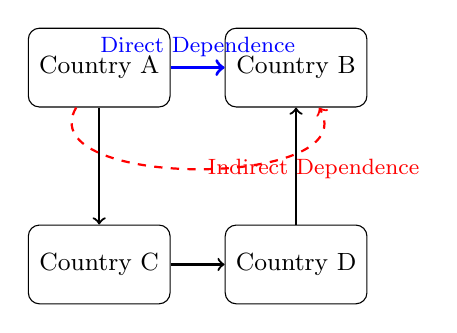
\begin{tikzpicture}[
    node distance=2.5cm,
    box/.style={rectangle, rounded corners, draw=black, minimum width=1.8cm, minimum height=1cm, text centered, font=\small},
    arrow/.style={->, thick}
]
    % Nodes
    \node[box] (A) {Country A};
    \node[box, right of=A] (B) {Country B};
    \node[box, below of=A] (C) {Country C};
    \node[box, below of=B] (D) {Country D};
    
    % Arrows
    \draw[arrow, blue, very thick] (A) -- (B) node[midway, above, font=\footnotesize] {Direct Dependence};
    \draw[arrow] (A) -- (C);
    \draw[arrow] (C) -- (D);
    \draw[arrow] (D) -- (B);
    
    % Curved arrow for indirect dependence
    \draw[arrow, red, dashed, thick] (A) to[out=240, in=300] node[midway, right, font=\footnotesize] {Indirect Dependence} (B);
\end{tikzpicture}
\caption{Schematic representation of direct and indirect dependencies in a simple trade network. Indirect dependencies (dashed red line) capture Country B’s exposure to Country A via intermediaries (Countries C and D).}
\label{fig:direct-indirect}
\end{figure}

The direct dependence (DD$_{ij}$) of country $j$ on country $i$ is formally defined as:

\begin{equation}
\text{DD}_{ij} = \frac{x_{ij}}{S_j}
\end{equation}

\noindent where:
\begin{itemize}
    \item $x_{ij}$ represents the value of trade flows from exporter $i$ (row) to importer $j$ (column)
    \item $S_j = \sum_{k} x_{kj}$ is the total supply of imports to country $j$ (column sum)
\end{itemize}

\textbf{Matrix Convention:} Throughout this paper, we adopt the convention that matrix $\mathbf{X}$ has exporters as rows and importers as columns. Thus, $x_{ij}$ denotes exports from country $i$ to country $j$. For computational efficiency, domestic production ($x_{jj}$, the diagonal elements) is excluded from our analysis, as we focus on international trade dependencies.

Indirect dependence (DI$_{ij}$) captures how country $j$ may depend on another country $i$ through third countries acting as intermediaries. Conceptually, this reflects situations where, for example, country $j$ imports components from country $k$, which in turn depends on inputs from country $i$. This second-order dependence and subsequent levels are not captured by traditional indicators, but can represent significant vulnerabilities.

For a trade path $p = (i, k_1, k_2, \ldots, k_{\ell-1}, j)$ that starts in exporter $i$, passes through intermediaries $k_1, k_2, \ldots, k_{\ell-1}$, and ends in importer $j$, we define the \textbf{path strength} $F(p)$ as the measure of how a disruption in country $i$ is transmitted to $j$ through this specific route. This transmission considers how the impact propagates and potentially attenuates as it passes through each intermediary.

\textbf{Normalized Transition Matrix:} To facilitate the calculation of path strengths, we first define the normalized transition matrix $\mathbf{T}$, where each element represents the proportion of country $j$

To address the complexity of these interdependencies, the proposed indicator integrates three complementary methodological frameworks:

\begin{itemize}
    \item \textbf{Input-Output Matrices:} Provide the fundamental structure to represent trade flows between countries and sectors. Following \citet{MillerBlair2009}, we use a matrix representation where each element $x_{ij}$ represents the value of imports from country $i$ to country $j$. This approach explicitly links trade flows with the production structure of each economy, capturing how dependencies arise from specific input needs.
    
    \item \textbf{Network Theory:} Conceptualizes international trade as a directed and weighted network where the nodes are countries, and the links represent trade flows. As noted by \citet{Fagiolo2010}, this approach allows for the analysis of structural properties such as centrality, connectivity, and community formation, revealing patterns of interdependence that are not evident in simple bilateral analyses. We apply concepts from graph theory to identify and quantify all possible paths through which a country may depend on another.
    
    \item \textbf{Shock Propagation Models:} Capture how a disruption in a node of the trade network propagates to others through multiple channels. Inspired by \citet{Bierkandt2014} and \citet{Cerina2015}, we develop an adaptive algorithm that models the transmission of vulnerabilities, considering dilution factors at each intermediate node. This approach reflects the fact that the impact of a disruption tends to attenuate as it moves through the network, but can also be amplified when it converges at critical nodes.
\end{itemize}

The integration of these three frameworks allows us to overcome key limitations identified in previous literature:

\begin{enumerate}
    \item \textbf{Systematic capture of indirect effects:} Unlike indicators focused solely on bilateral relationships, our approach explicitly models how dependencies are transmitted through intermediaries.
    
    \item \textbf{Consideration of the complete trade network structure:} Instead of analyzing isolated pairs of countries, we assess the position of each economy within the global trade system, identifying systemic vulnerabilities.
    
    \item \textbf{Precise quantification of dependency intensity:} The indicator not only identifies the existence of indirect dependencies but also quantifies their relative magnitude, allowing for the prioritization of policy intervention areas.
\end{enumerate}

This integrated approach is particularly relevant in the current context of geoeconomic fragmentation, where, as noted by \citet{Gopinath2024}, "connector countries" are emerging as bridges between geopolitically distant trade blocs. Our indicator explicitly identifies these critical nodes and evaluates their role in transmitting vulnerabilities across the global trade system.

The precise mathematical formulation that implements this conceptualization is developed in the next section, where we detail the specific algorithms used to calculate total dependence, integrating both direct and indirect components.


\subsection{Mathematical Formulation}

The calculation of the indicator is based on a matrix representation of international trade, where a matrix $X \in \mathbb{R}^{n \times n}$ describes the trade flows between $n$ countries. Each element $x_{ij}$ of the matrix represents the value of imports that country $j$ receives from country $i$.

\subsubsection{Calculation of Direct Dependence}

Direct dependence ($\text{DD}_{ij}$) of country $j$ on country $i$ is defined as the proportion of direct imports in the total supply:

\begin{equation}
\text{DD}_{ij} = \frac{\text{Imports from $i$ to $j$}}{\text{Total supply of $j$}} = \frac{x_{ij}}{S_j}
\end{equation}

where:
\begin{itemize}
    \item $x_{ij}$ represents the value of imports that country $j$ receives directly from $i$
    \item $S_j$ is the total supply of country $j$, which includes both its domestic production ($x_{jj}$) and all imports: $S_j = x_{jj} + \sum_{k\neq j} x_{kj}$
\end{itemize}

This formulation ensures that direct dependence is normalized between 0 and 1, facilitating comparisons between countries.

\subsubsection{Calculation of Indirect Dependence}

Indirect dependence ($\text{DI}_{ij}$) captures how country $j$ depends on country $i$ through intermediaries. It is calculated by summing the path strengths of all indirect trade routes (paths with length $\ell \geq 2$):

\begin{equation}
\text{DI}_{ij} = \sum_{p \in P_{ij}^{\ell \geq 2}} F(p)
\end{equation}

\noindent where:
\begin{itemize}
    \item $P_{ij}^{\ell \geq 2}$ is the set of all \textbf{simple paths} (without repeated nodes) from exporter $i$ to importer $j$ with path length at least 2
    \item $F(p)$ is the path strength defined in equation (5), measuring the transmission intensity of disruptions through that specific route
\end{itemize}

\textbf{Computational Implementation:} For efficiency, our algorithm treats paths of different lengths separately:
\begin{itemize}
    \item \textbf{Length 2 (vectorized):} For paths with a single intermediary $k$, we compute:
    \begin{equation}
    \text{DI}_{ij}^{(\ell=2)} = \sum_{k \neq i,j} T_{i,k} \cdot T_{k,j} = \sum_{k \neq i,j} \frac{x_{i,k}}{S_k} \cdot \frac{x_{k,j}}{S_j}
    \end{equation}
    This can be computed efficiently using matrix operations.
    
    \item \textbf{Length $\ell \geq 3$ (enumeration):} For longer paths, we use explicit enumeration over combinations of intermediaries, computing $F(p)$ for each valid path and summing contributions.
\end{itemize}

For a trade path $p = (i, k_1, k_2, ..., k_n, j)$ that starts in country $i$, passes through intermediaries $k_1, k_2, ..., k_n$, and ends in country $j$, we calculate its strength by considering how dependence "dilutes" as it passes through each intermediary:

The path strength is computed as the product of transition probabilities along each edge of the path:

\begin{equation}
F(p) = \prod_{(a,b) \in \text{edges}(p)} T_{ab}
\end{equation}

\noindent For the complete path $p = (i, k_1, k_2, \ldots, k_{\ell-1}, j)$, this expands to:

\begin{equation}
F(p) = T_{i,k_1} \cdot T_{k_1,k_2} \cdots T_{k_{\ell-1},j} = \frac{x_{i,k_1}}{S_{k_1}} \cdot \frac{x_{k_1,k_2}}{S_{k_2}} \cdots \frac{x_{k_{\ell-1},j}}{S_j}
\end{equation}

\noindent where $\ell$ is the path length (number of edges). This formulation captures how a supply disruption originating in country $i$ would propagate through the chain to ultimately affect country $j$, with the impact potentially attenuating at each intermediary depending on their supplier diversification (reflected in the denominator $S_k$).

\subsubsection{Convergence and Relevance Criteria}

In theory, the number of possible trade paths between two countries can be infinite in a network with cycles. Additionally, the practical value of considering extremely long paths or those with marginal contributions is limited. Therefore, to ensure computational tractability and the economic relevance of the indicator, we incorporate three important methodological criteria.

The first is a trade relevance threshold ($\theta$), which establishes that only trade flows representing at least $\theta\%$ of total global trade are considered. This threshold, typically set between 0.05\% and 0.1\%, helps filter marginal trade relationships that could introduce noise into the analysis without adding substantial information. Applying this threshold transforms the dense matrix of global trade into a more sparse but meaningful representation, focusing on economically relevant flows.

The second criterion is a convergence threshold ($\varepsilon$), which determines when to stop the calculation of indirect dependencies. The iterative process is halted when the inclusion of additional paths does not significantly alter the total dependency value beyond this threshold (typically 0.01). This criterion reflects the empirical observation that extremely long or complex paths have a diminishing marginal contribution to total dependence. In practice, this means that, for most country pairs, only a limited number of paths need to be considered to obtain an accurate estimate of dependence.

The third criterion introduces a maximum path length ($L_{\max}$), which, for computational efficiency, limits the search for trade paths to a maximum number of intermediaries (typically between 3 and 5). Numerous empirical studies on global value chains suggest that this limit is sufficient to capture the main indirect dependencies in most trade networks, without significantly compromising the accuracy of the indicator.

These criteria are implemented in an adaptive algorithm that calculates indirect dependence iteratively. Formally, we define:

\begin{equation}
\text{DI}_{ij}^{(l)} = \sum_{p\in P_{ij}^{(l)}} F(p)
\end{equation}

where $P_{ij}^{(l)}$ is the set of paths of length exactly $l$ between countries $i$ and $j$. The algorithm proceeds iteratively, calculating $\text{DI}_{ij}^{(1)}$, $\text{DI}_{ij}^{(2)}$, and so on. It stops when $|\text{DI}_{ij}^{(l)} - \text{DI}_{ij}^{(l-1)}| < \varepsilon$ or when $l = L_{\max}$. This approach ensures that the calculation is computationally efficient while capturing the most significant indirect dependencies.

\subsubsection{Total Dependence}

Total dependence ($\text{DT}_{ij}$) of country $j$ on country $i$ is defined as the sum of both direct and indirect components:

\begin{equation}
\text{DT}_{ij} = \text{DD}_{ij} + \text{DI}_{ij}
\end{equation}

This formulation offers several desirable properties for a trade vulnerability indicator. First, $\text{DT}_{ij}$ is bounded in the interval $[0, 1]$, facilitating the interpretation and comparability of results. Second, the difference $\text{DT}_{ij} - \text{DD}_{ij}$ provides a direct measure of the "hidden" vulnerability that would not be captured by conventional bilateral analyses. Third, when no significant indirect paths exist between $i$ and $j$, we have $\text{DT}_{ij} \approx \text{DD}_{ij}$, meaning the indicator naturally reduces to the bilateral case when indirect dependencies are negligible.

The interpretation of the indicator is straightforward and intuitive: $\text{DT}_{ij}$ represents the proportion of country $j$’s total supply that depends, directly or indirectly, on country $i$. A high value indicates significant vulnerability to disruptions in country $i$, while values close to $\text{DD}_{ij}$ suggest that indirect dependencies are marginal. This interpretation facilitates the communication of results to policymakers and its application in economic security analysis contexts.

It is important to note that, unlike other indicators, $\text{DT}_{ij}$ is not simply a measure of trade exposure, but a specific quantification of vulnerability to supply disruptions. Its design explicitly incorporates the structure of the global trade network and shock propagation mechanisms, providing a more comprehensive and nuanced view of the economic interdependencies that characterize contemporary international trade.

\subsection{Computational Implementation and Practical Considerations}

The practical application of the indicator to real trade data requires addressing a number of significant computational challenges. The complexity of global trade networks, which can involve hundreds of countries and thousands of sectors, demands efficient implementation strategies that allow for the calculation of direct and indirect dependencies in reasonable time frames. In this section, we detail the key technical aspects of our implementation.

Enumerating paths in trade networks is perhaps the most important challenge. For realistically sized networks, the number of potential paths between pairs of countries grows exponentially with the maximum allowed path length. A brute-force approach that attempts to enumerate all possible paths would be computationally unfeasible even for moderate-sized networks. To overcome this limitation, we have developed an adaptive algorithm that explores the path space efficiently.

Our approach begins by identifying the shortest and most commercially significant paths, which typically represent the most significant indirect dependencies. We use a modified breadth-first search variant that prioritizes links with higher economic relevance. This strategy enables the quick identification of the paths that contribute most to indirect dependence. Subsequently, the relevance threshold is applied to eliminate paths whose contribution would be marginal, significantly reducing the search space.

To further optimize the process, we employ memoization techniques that store intermediate results of subpaths that have already been calculated. This avoids redundant computations in networks where multiple paths share common segments, a feature common in trade networks where certain countries act as regional hubs. As we explore longer paths, the algorithm iteratively refines the dependence estimate, stopping when convergence is reached according to the established criteria.

Efficient handling of sparse matrices is another key aspect of our implementation. International trade matrices naturally exhibit a high degree of sparsity: most countries trade significantly only with a relatively small subset of partners. This feature is accentuated when trade relevance thresholds are applied. Exploiting this sparsity is crucial for computational efficiency.

Our implementation uses specialized data structures for sparse matrices, explicitly representing only the non-zero elements of the trade matrix. This dramatically reduces memory requirements, enabling the analysis of detailed trade networks even with limited computational resources. Additionally, we implement optimized algorithms for sparse matrix algebra, particularly for key operations such as matrix-vector multiplication used in the recursive calculation of indirect dependencies.

For extensive historical data sets, we apply selective data compression techniques that preserve accuracy in the most relevant trade flows while reducing detail in marginal connections. This approach enables longitudinal analyses spanning decades of trade data without sacrificing computational efficiency.

The nature of the dependency calculation problem lends itself naturally to parallelization, offering significant opportunities to reduce processing times. We observe that the dependency between a specific pair of countries $(i,j)$ can be calculated independently of other pairs, allowing for efficient distribution of work across multiple processors or cores.

Our parallelized implementation decomposes the global dependency matrix into submatrices that are computed concurrently. A central coordinator distributes these tasks across the available processors, implementing dynamic load balancing strategies that assign more resources to more complex calculations (typically those involving countries with many trade links). The partial results are then combined to construct the complete dependency matrix.

In distributed computing environments, we minimize communication between processes, transmitting only the essential information for each calculation. This strategy significantly reduces the overhead associated with coordinating parallel processes. The scalability of our implementation has been empirically validated: the computation time scales nearly linearly with the number of available processors up to approximately 64 cores, allowing detailed global network analyses in minutes rather than days.

The robustness of the indicator against variations in the calculation parameters and input data quality is a legitimate concern for any quantitative methodology. To address this, we have implemented extensive validation procedures that verify the stability and reliability of our results.

Sensitivity analysis with respect to key parameters ($\theta$, $\varepsilon$, and $L_{\max}$) confirms that, for reasonable ranges of values, the main conclusions derived from the indicator remain stable. Moderate variations in these parameters may affect specific numerical values, but rarely alter the relative ordering of dependencies or the identification of critical vulnerabilities. This robustness reinforces the practical usefulness of the indicator in informing economic policy decisions.

To validate the algorithm’s performance, we have conducted tests with synthetic networks of known structure, where theoretical dependencies can be calculated analytically. These experiments confirm that our implementation correctly recovers the expected dependencies, even in cases involving complex connectivity patterns. Additionally, for specific data subsets where alternative dependency measures exist, we have verified that our indicator produces results consistent with these external references.

Perhaps the most convincing validation comes from historical case studies. We have analyzed documented episodes of trade disruptions, such as the 2011 Japan earthquake and tsunami or certain phases of the U.S.-China trade war, retrospectively evaluating the predictive capacity of the indicator. These analyses confirm that countries with high total dependence values (especially those with significant indirect components) indeed experienced greater economic impacts during these disruptive episodes.

\subsection{Advantages of the Proposed Indicator}

The trade dependence indicator we propose offers substantial advantages over traditional metrics, particularly in the current context of the geopolitical reconfiguration of international trade. These advantages stem from both its robust theoretical foundation and its design aimed at capturing the complexity of contemporary trade interdependencies.

The systematic capture of indirect effects is perhaps the most significant contribution of our approach. Conventional indicators, by focusing solely on direct bilateral flows, provide a partial and potentially misleading view of actual trade vulnerabilities. Our model, in contrast, incorporates all relevant indirect trade paths, revealing dependencies that would remain hidden in simple bilateral analyses. This feature is especially valuable in the current landscape of highly fragmented global value chains, where countries rarely depend solely on direct trading partners.

The ability to identify and quantify these hidden dependencies allows for a much more precise assessment of the risks associated with disruptions in specific countries. As noted by several empirical studies, including those by \citet{Vicard2023}, evaluations based solely on bilateral trade can significantly underestimate actual exposure to supply risks. Our indicator corrects this deficiency by explicitly modeling how potential disruptions propagate across the entire trade network, even reaching distant partners via intermediaries.

The dynamic assessment of economic resilience represents another key advantage of the proposed indicator. By explicitly modeling shock propagation mechanisms in the global trade network, our approach enables the analysis of dynamic scenarios where disruptions are sequentially transmitted between countries. This allows for the study of how an adverse event in a specific node of the trade network can trigger cascading effects that affect economies seemingly disconnected from the shock's origin.

This analytical capacity is crucial in an environment where, as documented by \citet{Baldwin2020}, trade disruptions frequently generate "contagion waves" that spread across multiple countries and sectors. Our indicator provides tools to anticipate these propagation patterns, identify potential vulnerability points, and assess the effectiveness of different strategies to enhance the resilience of the trade system. The application of this approach to recent crises, such as supply disruptions during the COVID-19 pandemic, has confirmed its ability to identify transmission channels that conventional analyses failed to anticipate.

The coherent integration of Input-Output models and network theory is a distinctive methodological aspect of our approach. While traditional Input-Output matrix-based analyses focus on quantifiable economic flows but often ignore the topological structure of the trade network, network studies capture structural properties but usually lack direct linkage to economic magnitudes. Our indicator overcomes this dichotomy by combining both perspectives into a unified framework.

This integration enables multidimensional analysis that simultaneously considers the topological structure of the trade network, the magnitude of economic flows, and the mechanisms of disruption propagation. As \citet{Cerina2015} argue, this type of hybrid approach is particularly well-suited for characterizing complex systems like contemporary international trade, where a country’s structural position within the network can be as important as the volume of its bilateral exchanges.

The formal properties of the indicator facilitate its interpretation and practical application. Normalization in the interval [0, 1] allows for direct comparisons between different countries, sectors, and time periods. This is especially useful for policymakers and analysts who need to identify and prioritize critical vulnerabilities in a context of limited resources. The explicit separation between direct and indirect components of dependence provides additional information about the nature of vulnerabilities, allowing for more precise and effective policy responses.

Unlike complex indicators with abstract interpretations, our indicator maintains a direct connection to the underlying economic reality: it represents the proportion of a country’s total supply that depends, directly or indirectly, on another country. This intuitive interpretation facilitates the communication of results to non-specialized audiences and their incorporation into decision-making processes.

Despite the underlying conceptual complexity, the indicator has been designed to ensure computational efficiency. Optimized algorithms allow for its calculation on detailed global trade networks using moderate computational resources, facilitating its regular update as new data becomes available. This computational efficiency is crucial for continuous vulnerability monitoring and near-real-time scenario analysis.

The practical applicability of the indicator extends to various institutional contexts. For governments and supranational institutions, such as the European Union in its pursuit of "open strategic autonomy" (ECB, 2023), it provides an analytical tool to identify critical dependencies and assess diversification strategies. For multinational corporations, it offers a framework for analyzing risks in increasingly complex global supply chains, complementing existing approaches such as those proposed by \citet{StollThethi2022}. For international organizations monitoring the fragmentation of global trade, such as the IMF (Gopinath et al., 2024), it provides accurate quantitative metrics for assessing the evolution of trade interdependencies in a context of growing geopolitical polarization.

Together, these advantages make the proposed indicator particularly suitable for the analysis of economic security in the current environment, characterized by growing geopolitical tensions, reorganization of global value chains, and reevaluation of strategic dependencies. Its ability to identify hidden vulnerabilities, quantify systemic risks, and evaluate mitigation strategies makes it a valuable tool for informing policies that seek to balance the benefits of trade integration with the imperatives of national economic security.

Table \ref{tab:comparacion-metodos} compares the main approaches used to measure trade dependence, evaluating their capabilities across fourteen key dimensions: inclusion of indirect dependence, normalization, reliance on Input-Output models, use of network theory, and applicability in economic security analysis, among others.

\begin{table}[!t] 
\caption{Comparison of Methods for Measuring Trade Dependence} \label{tab:comparacion-metodos} 
\centering 
\footnotesize
\renewcommand{\arraystretch}{1.1} 
\begin{adjustbox}{width=\textwidth,center}
    \begin{tabular}{@{}l*{6}{c}@{}} 
        \toprule 
        \makecell[l]{\textbf{Characteristic}} & \textbf{HHI} & \makecell{\textbf{Conc.}\\\textbf{Imp.}} & \textbf{TiVA} & \makecell{\textbf{I-O}\\\textbf{Trad.}} & \makecell{\textbf{Net-}\\\textbf{works}} & \makecell{\textbf{Proposed}\\\textbf{Ind.}} \\ 
        \midrule 
        Captures direct dep. & \textcolor{green!70!black}{\checkmark} & \textcolor{green!70!black}{\checkmark} & \textcolor{green!70!black}{\checkmark} & \textcolor{green!70!black}{\checkmark} & \textcolor{green!70!black}{\checkmark} & \textcolor{green!70!black}{\checkmark} \\ 
        Captures indirect dep. & \textcolor{red!70!black}{\texttimes} & \textcolor{red!70!black}{\texttimes} & \textcolor{orange!90!black}{Partial} & Direct only & \textcolor{green!70!black}{\checkmark} & \textbf{\textcolor{green!70!black}{Complete}} \\ 
        Normalization (0-1) & \textcolor{green!70!black}{\checkmark} & \textcolor{green!70!black}{\checkmark} & \textcolor{red!70!black}{\texttimes} & \textcolor{red!70!black}{\texttimes} & \textcolor{red!70!black}{\texttimes} & \textcolor{green!70!black}{\checkmark} \\
        Based on Input-Output & \textcolor{red!70!black}{\texttimes} & \textcolor{red!70!black}{\texttimes} & \textcolor{green!70!black}{\checkmark} & \textcolor{green!70!black}{\checkmark} & \textcolor{red!70!black}{\texttimes} & \textcolor{green!70!black}{\checkmark} \\ 
        Network theory & \textcolor{red!70!black}{\texttimes} & \textcolor{red!70!black}{\texttimes} & \textcolor{red!70!black}{\texttimes} & \textcolor{red!70!black}{\texttimes} & \textcolor{green!70!black}{\checkmark} & \textcolor{green!70!black}{\checkmark} \\ 
        Models shock propagation & \textcolor{red!70!black}{\texttimes} & \textcolor{red!70!black}{\texttimes} & \textcolor{red!70!black}{\texttimes} & \textcolor{orange!90!black}{Limited} & \textcolor{orange!90!black}{Partial} & \textcolor{green!70!black}{\checkmark} \\ 
        Detects hidden vuln. & \textcolor{red!70!black}{\texttimes} & \textcolor{red!70!black}{\texttimes} & \textcolor{orange!90!black}{Partial} & \textcolor{red!70!black}{\texttimes} & \textcolor{orange!90!black}{Partial} & \textcolor{green!70!black}{\checkmark} \\ 
        Resilience analysis & \textcolor{red!70!black}{\texttimes} & \textcolor{red!70!black}{\texttimes} & \textcolor{orange!90!black}{Limited} & \textcolor{orange!90!black}{Limited} & \textcolor{orange!90!black}{Partial} & \textcolor{green!70!black}{\checkmark} \\ 
        \bottomrule 
    \end{tabular}
\end{adjustbox}
\begin{tablenotes} 
\scriptsize 
\item \textit{Notes:} HHI: Herfindahl-Hirschman Index; Conc. Imp.: Import Concentration Index; TiVA: Trade in Value Added; I-O Trad.: Traditional Input-Output Models; Networks: Network Analysis; Proposed Ind.: This paper's indicator.
\end{tablenotes} 
\end{table}



Trade in Value Added (TiVA) offers a partial improvement by tracking the contribution of each country within global production, but it does not explicitly model how shocks propagate through the trade network. As noted by \citet{Koopman2014} (p.459-460), "traditional trade statistics are increasingly unreliable as indicators of the value added by any particular country" because "intermediate inputs cross borders multiple times."

On the other hand, traditional Input-Output models allow for the evaluation of sectoral interdependencies but do not incorporate a global trade network structure that represents the propagation of indirect dependencies. \citet{Cerina2015} (p.9) emphasize that "the fact that industries are both highly connected and asymmetrically connected means that local idiosyncratic shocks can propagate throughout the global economy," an aspect that these models fail to capture adequately.

Network analysis, such as the approach by \citet{Korniyenko2017}, provides a structural visualization of international trade, detecting commercial hubs and centrality patterns. However, because it is not based on Input-Output matrices, it does not accurately quantify the flow of productive inputs nor provide a direct economic interpretation of trade dependence.

The proposed index overcomes these limitations by integrating the most relevant elements of Input-Output models and network analysis into a single methodological framework, also incorporating shock propagation algorithms. This combination allows for the identification of hidden dependencies that traditional approaches fail to detect, as evidenced by \citet{SimchiLevi2015}, who discovered that "some of the greatest exposures reside in unexpected places, such as non-strategic suppliers" (p.379-380).

Table \ref{tabla:comparacion_metodos} compares the main approaches used to measure trade dependence, evaluating their capabilities across four key dimensions: inclusion of indirect dependence, reliance on Input-Output models, use of network theory, and applicability in economic security analysis.

The Herfindahl-Hirschman Index (HHI) and Import Concentration Index are widely used to measure supplier concentration, but they present a critical limitation: their inability to capture trade dependencies transmitted through third countries. This can lead to an underestimation of risks when interdependencies are not evident in bilateral analyses.

Trade in Value Added (TiVA) offers a partial improvement by tracking each country’s contribution to global production, but it does not explicitly model how shocks propagate through the trade network. On the other hand, traditional Input-Output models allow for the evaluation of sectoral interdependencies but fail to incorporate a global trade network structure that represents the propagation of indirect dependencies.

Network analysis, such as the approach by \citet{Korniyenko2017}, provides a structural visualization of international trade, detecting commercial hubs and centrality patterns. However, because it is not based on Input-Output matrices, it does not accurately quantify the flow of productive inputs nor provide a direct economic interpretation of trade dependence.

The proposed index overcomes these limitations by integrating the most relevant elements of Input-Output models and network analysis into a single methodological framework, also incorporating shock propagation algorithms. This combination allows for:

\begin{itemize}
    \item Identifying \textit{hidden dependencies} that traditional approaches do not detect.
    \item Capturing both the intensity and structure of trade interdependencies.
    \item Quantitatively assessing how trade shocks can propagate across multiple levels of intermediaries.
\end{itemize}

Thanks to these improvements, the proposed indicator stands as a more suitable tool for assessing trade vulnerability in a context of growing geoeconomic fragmentation. Its application in policy design will enable governments and international organizations to develop more effective strategies to mitigate trade risks, strengthen supply chain resilience, and ensure economic security in an uncertain global environment.

\subsection{Applications and Current Relevance}

In the current geopolitical context, characterized by growing trade tensions and a reconfiguration of global value chains, the proposed indicator offers highly valuable applications for various institutional actors. Its ability to capture indirect dependencies is particularly relevant at a time when economic security considerations have risen on the international political agenda.

The identification of strategic vulnerabilities is perhaps the most immediate application of the indicator. National governments and supranational organizations can use this methodology to detect critical dependencies that could compromise their economic security in the face of disruptions in international trade. Unlike traditional analyses, our approach reveals not only the obvious vulnerabilities derived from direct trade relations but also those "hidden" vulnerabilities that manifest through intermediaries.

This aspect is especially relevant for economies like the European Union, where recent analyses by the European Commission (2021) have highlighted the need to develop more sophisticated tools to identify strategic dependencies. The indicator we propose complements these efforts by providing a more comprehensive and nuanced view of European trade vulnerabilities, particularly in critical sectors such as semiconductors, essential raw materials, or pharmaceuticals.

The assessment of diversification policies represents another highly valuable application. Policymakers frequently face the complex task of designing strategies to reduce trade vulnerabilities without sacrificing the benefits of specialization and international trade. Our indicator provides an analytical framework for simulating and evaluating the impact of different supplier diversification strategies, allowing for the identification of those that offer the greatest reductions in vulnerability with the lowest economic costs.

For example, the indicator allows for distinguishing between "superficial" diversification (redistributing direct imports among suppliers that share the same indirect vulnerabilities) and "deep" diversification (which effectively reduces dependence on common sources across the entire supply chain). This distinction is crucial for designing effective policies, especially in a context where, as pointed out by \citet{Alfaro2023}, there is a significant relocation of production chains driven by geopolitical considerations.

Sectoral resilience analysis is a third relevant application of our methodology. The indicator allows for a comparative assessment of different industrial sectors' vulnerability to trade disruptions, identifying those sectors that are most exposed to supply risks. This information is valuable for prioritizing industrial policy interventions and developing strategic productive capacities in particularly vulnerable areas.

Our preliminary empirical analyses, applying the indicator to detailed sectoral data, reveal heterogeneous patterns of vulnerability across sectors. Industries such as advanced electronics, certain pharmaceuticals, and emerging green technologies tend to show particularly high indirect dependencies, often concentrated in a small number of original suppliers. These findings align with the observations by \citet{Arriola2024} on the existence of "critical vulnerabilities" in specific value chains, but our approach provides a more precise quantification and better identification of indirect transmission channels.

Monitoring the temporal evolution of dependencies represents another valuable application of the proposed indicator. By systematically calculating dependency matrices for different periods, it is possible to identify worrying trends before they become critical vulnerabilities. This "early warning" approach allows for more effective and less costly preventive interventions than reactive responses to already materialized crises.

In this regard, our indicator contributes to what \citet{Ioannou2021} and \citet{Perez2021} term "structural surveillance" in the economic field: the proactive identification of potential sources of instability before they generate significant disruptions. This capability is particularly valuable in a context of growing geopolitical fragmentation, where the reconfiguration of trade alliances can quickly alter established dependency patterns.

The evaluation of the potential impact of geopolitical conflicts on third countries constitutes an additional application that is especially relevant in the current context. The indicator allows for modeling how tensions or conflicts between certain actors could indirectly affect seemingly uninvolved countries through complex trade channels. This analytical capability is valuable for formulating mitigation strategies and contingency plans in the face of commercial fragmentation scenarios.

For example, our approach can assess how a hypothetical escalation of tensions between the United States and China would affect intermediary economies such as Mexico, Vietnam, or Singapore, which currently act as "bridge countries" between increasingly distant trade blocs. This type of scenario analysis provides crucial information for managing geopolitical risks, both for governments and multinational companies with global supply chains.

Together, these applications address urgent needs for sophisticated analytical tools at a time when, as \citet{Gopinath2024} point out, international trade is experiencing significant structural transformations driven by considerations that go beyond purely economic logic. The indicator we propose not only identifies existing vulnerabilities but also provides a framework for anticipating future reconfigurations and developing adaptation strategies in an increasingly complex and geopolitically fragmented trade environment.

\subsection{Implications for Economic Security}

The theoretical and methodological framework we have developed has profound implications for the conceptualization, measurement, and management of economic security in the current context. These implications extend beyond the purely technical aspect of measuring trade dependencies, reaching strategic considerations about the vulnerability of economies to exogenous disruptions and the design of policies to strengthen resilience.

The identification of hidden vulnerabilities is perhaps the most direct and significant implication of our approach. By systematically capturing the indirect dependencies transmitted through trade intermediaries, the proposed indicator reveals vulnerabilities that would remain invisible in analyses focused solely on bilateral relations. This more comprehensive "mapping" of the terrain of economic interdependencies allows for a more realistic assessment of the risks associated with the current configuration of international trade.

Case studies we have conducted applying our methodology to strategic sectors illustrate the magnitude of these hidden vulnerabilities. For example, in the field of rare earths, critical components for green technologies and defense applications, we discovered that the effective dependence of many European countries on China is substantially higher than suggested by direct trade statistics. This is because important processing intermediaries in Asia and North America also depend on Chinese raw materials, creating an indirect vulnerability that conventional indices such as the HHI fail to capture.

These findings align with the observations of \citet{Campbell2024} on how disruptions in specific nodes of supply chains can propagate globally, affecting economies that seem diversified in terms of direct suppliers. Our indicator provides a precise quantitative measure of this exposure, enabling systematic comparisons across countries, sectors, and time periods.

The assessment of contagion risks represents another fundamental implication of our methodology. The explicit modeling of trade paths allows us to analyze how disruptions in one node of the network can propagate through multiple channels, creating systemic effects that exceed the sum of bilateral relations. This "systemic risk" perspective in international trade complements similar approaches developed in the financial sector after the global crisis of 2008.

Our methodology allows for the identification of "critical nodes" in the global trade network: countries or sectors whose disruption would have disproportionately large effects due to their strategic position as intermediaries in multiple value chains. These nodes do not always coincide with the largest economies or the largest exporters; instead, they often include specialized countries that occupy critical niches in particular production chains.

For example, preliminary analyses applying our indicator to recent trade data suggest that economies such as Singapore, South Korea, Taiwan, and increasingly Vietnam play particularly important roles as transmitters of dependencies in advanced technological sectors. Identifying these critical nodes provides valuable information for managing systemic risks in global trade, allowing for the anticipation of propagation patterns in the face of localized disruptions.

The design of mitigation policies constitutes a third area where our methodology has significant implications. The decomposition of dependence into direct and indirect components facilitates the design of differentiated strategies to address different types of vulnerability. While direct dependencies can be mitigated by diversifying immediate suppliers, indirect dependencies often require more complex interventions, such as the development of domestic productive capacities in critical links of the chain or trade agreements with suppliers who present complementary dependency profiles.

This distinction is particularly relevant in the context of "open strategic autonomy" policies being developed by actors such as the European Union. As the European Central Bank (2023) notes, the goal is not economic autarky but the intelligent management of interdependencies that minimizes critical vulnerabilities without unnecessarily sacrificing the benefits of trade openness. Our indicator provides precise analytical tools for this balance, allowing for the identification of areas where intervention is a priority and evaluating the potential effectiveness of different strategies.

The dynamic monitoring of the evolution of dependencies represents another practical implication of our methodology. The mathematical convergence of the indicator and its computationally efficient implementation allow for its regular application to continuously track how trade vulnerabilities evolve over time. This monitoring is particularly valuable in a context where, as \citet{Frohm2022} and \citet{Gunnella2022} document, global value chains are undergoing significant reconfigurations driven both by disruptive events (such as the COVID-19 pandemic) and by long-term strategic considerations.

The ability to systematically update dependency matrices as new trade data becomes available allows for the evaluation of whether implemented policies are effectively reducing critical vulnerabilities or whether new problematic dependency patterns are emerging. This dynamic evaluation capability facilitates the continuous adaptation of strategies in response to an increasingly volatile and uncertain trade environment.

In broader terms, our advanced conceptualization of trade dependence provides a more solid foundation for the development of economic security strategies tailored to the current context. As \citet{Balteanu2025} argues, the very notion of economic security is evolving from narrow concepts focused on specific sectors to systemic approaches that consider the resilience and adaptability of the economic system as a whole.

Our methodology contributes to this conceptual evolution by providing tools that allow for the visualization and quantification of the complex interconnections characterizing the contemporary global economy. The emphasis on indirect dependencies and systemic effects broadens the traditional perspective on trade vulnerabilities, facilitating a more informed balance between the benefits of global integration and the imperatives of national or regional economic security.

Finally, the proposed indicator has significant implications for assessing trade fragmentation scenarios, an increasingly relevant aspect in the current geopolitical context. As \citet{Campos2023} notes, the growing divergence between geopolitical blocs is generating pressures toward a partial reorganization of international trade along lines of political affinity rather than economic complementarity.

Our methodology allows for the modeling of alternative fragmentation scenarios, evaluating how different patterns of trade reorganization would affect the vulnerabilities of specific countries. These prospective analyses provide valuable information for formulating adaptive strategies that aim to minimize the economic costs of fragmentation while preserving adequate levels of security in the supply of critical goods and services.

Together, these implications form an integrated framework for rethinking economic security in an era of growing geopolitical uncertainty. The indicator we propose not only offers a more accurate and comprehensive measure of existing trade vulnerabilities, but also provides analytical tools to anticipate and manage emerging risks in an increasingly complex and interconnected international system.
Here is the translation of the requested section into academic English:


\section{Analysis of Centrality and Critical Intermediaries in Trade Networks}

\subsection{Relevance and Applications}

The analysis of centrality and identification of critical intermediaries in international trade networks represents a fundamental methodological extension for understanding the true nature of economic vulnerabilities. While traditional trade dependency measures primarily focus on direct bilateral relations, this approach captures the structural complexity of contemporary global value chains, where a significant number of trade exchanges occur through intermediary countries.

The systematic identification of these critical intermediaries offers multiple analytical advantages:

\begin{itemize}
    \item \textbf{Detection of hidden vulnerabilities}: It reveals indirect dependencies that would remain invisible in conventional bilateral analyses, providing a more comprehensive assessment of supply risks.
    
    \item \textbf{Assessment of systemic risks}: It identifies critical points whose disruption could create cascading effects across multiple supply chains, impacting economies that appear to be disconnected.
    
    \item \textbf{Strategic diversification}: It facilitates the design of supplier diversification strategies that consider not only the direct source of imports but also the indirect trade routes.
    
    \item \textbf{Economic geopolitics}: It identifies countries that, due to their position as intermediaries in multiple value chains, hold disproportionate economic influence relative to their size.
\end{itemize}

In the current context of growing geopolitical fragmentation, where divergent trade blocs seek reorganization along lines of political affinity, the role of intermediaries takes on unprecedented relevance. Countries acting as "connectors" between different spheres of influence can become strategic choke points or, alternatively, enablers of global trade resilience.

Sectoral analysis of these intermediaries is particularly valuable, as different industries exhibit distinct commercial network structures. Sectors such as semiconductors, critical minerals, or pharmaceuticals tend to be characterized by high degrees of specialization and geographic concentration, creating specific intermediary patterns that warrant detailed examination.

\subsection{Mathematical Formulation}

To integrate the analysis of critical intermediaries into our economic security indicator, we propose a methodology combining elements of network theory, dependency propagation, and centrality metrics. Below, we formally develop this methodological extension.

\subsubsection{Identification of Critical Routes}

First, we extend the calculation of indirect dependency to not only capture the aggregated value of this dependency but also the specific routes through which it is transmitted. For each pair of countries $(i,j)$ and each possible route length $\ell$, we identify the set of significant trade routes $\mathcal{P}_{ij}^{\ell}$.

A route $p = (p_1, p_2, \ldots, p_{\ell+1})$ of length $\ell$, where $p_1 = j$ (exporter) and $p_{\ell+1} = i$ (importer), is considered significant if its strength $F(p)$ exceeds a predefined threshold $\theta_p$:

\begin{equation}
F(p) > \theta_p
\end{equation}

where the strength of a route is defined as:

\begin{equation}
F(p) = \prod_{k=1}^{\ell} \frac{x_{p_k p_{k+1}}}{S_{p_{k+1}}}
\end{equation}

where $x_{p_k p_{k+1}}$ is the trade flow from country $p_k$ to country $p_{k+1}$, and $S_{p_{k+1}}$ is the total supply received by country $p_{k+1}$. This formulation captures the transmission of dependencies through multiple intermediary countries.

**\subsubsection{Centrality Metrics for Intermediaries}**

For each country $k$, we calculate two fundamental metrics that capture its importance as an intermediary:

\begin{itemize}
    \item \textbf{Intermediation Frequency} ($\phi_k$): Counts how many significant trade routes country $k$ participates in as an intermediary:
    
    \begin{equation}
    \phi_k = \sum_{i,j} \sum_{\ell=2}^{L_{\max}} \sum_{p \in \mathcal{P}_{ij}^{\ell}} \mathbb{1}_{k \in p \setminus \{p_1, p_{\ell+1}\}}
    \end{equation}
    
    where $\mathbb{1}$ is the indicator function that equals 1 if country $k$ is an intermediary in route $p$ (excluding the exporter $p_1$ and the importer $p_{\ell+1}$).
    
    \item \textbf{Intermediation Strength} ($\psi_k$): A weighted sum that captures the economic importance of the routes in which country $k$ participates:
    
    \begin{equation}
    \psi_k = \sum_{i,j} \sum_{\ell=2}^{L_{\max}} \sum_{p \in \mathcal{P}_{ij}^{\ell}} F(p) \cdot w(k,p) \cdot \mathbb{1}_{k \in p \setminus \{p_1, p_{\ell+1}\}}
    \end{equation}
    
    where $w(k,p)$ is a weighting factor that assigns more importance to intermediaries closer to the final importer:
    
    \begin{equation}
    w(k,p) = \frac{1}{d(k, p_{\ell+1})}
    \end{equation}
    
    where $d(k, p_{\ell+1})$ is the distance (number of steps) between intermediary $k$ and the final importer $p_{\ell+1}$ in route $p$.
\end{itemize}

Here is the translation of the requested section into academic English:

---

**\subsubsection{Composite Centrality Index}**

Finally, we define a composite centrality index for each country $k$ that integrates both normalized metrics:

\begin{equation}
C_k = \alpha \cdot \frac{\phi_k}{\max_i \phi_i} + (1-\alpha) \cdot \frac{\psi_k}{\max_i \psi_i}
\end{equation}

where $\alpha \in [0,1]$ is a parameter that determines the relative weight of the frequency versus the strength of intermediation. Empirically, we have found that a value of $\alpha = 0.4$ provides an optimal balance between both dimensions.

This centrality index $C_k \in [0,1]$ allows for the ranking of countries according to their importance as intermediaries in global trade, thereby complementing the analysis of direct and indirect dependencies.

**\subsection{Sectorial Application}**

To apply this methodology at the sectorial level, we calculate the centrality index $C_k^s$ for each sector $s$ independently. This allows us to identify specific patterns of intermediation by industry and reveal sectorial vulnerabilities that might be diluted in an aggregated analysis.

Comparing these sectorial indices facilitates the identification of:

\begin{itemize}
    \item Countries with high specialization as intermediaries in specific strategic sectors.
    \item Sectors with higher concentration of intermediation versus those with more diversified trade routes.
    \item Correlations between centrality in different sectors, revealing possible interdependencies between seemingly disconnected supply chains.
\end{itemize}

This methodological extension represents a significant contribution to the assessment of economic security, providing more robust analytical tools to understand and manage the risks derived from the increasing complexity of global trade networks.


\section{Simulation of Disruptions in the Global Trade Network}

To evaluate the impact of trade disruptions, a simulation of counterfactual scenarios is implemented, focusing on the removal or alteration of key nodes within the global trade network. This approach allows us to measure the structural vulnerability of international trade relations and provides relevant information for identifying potential risks and mitigation strategies. The simulation is organized in the following steps:

\begin{enumerate}
    \item \textbf{Definition of the System to Simulate:} The global trade system is modeled as a network, where the \textit{nodes} correspond to countries or economic sectors, and the \textit{links} represent bilateral or multilateral trade flows between them. This network is constructed using international trade data, especially those affected by recent tariff measures.
    
    \item \textbf{Removal of Key Nodes:} Critical nodes within the trade network are identified, those whose trade is essential for other countries or sectors. These key nodes can include countries like China or industrial sectors like battery production. In counterfactual scenarios, these nodes are removed from the network to simulate trade disruptions, such as economic sanctions or supply chain interruptions.
    
    \item \textbf{Simulation of Changes in Links:} In addition to removing nodes, changes in trade links are simulated. This may involve the reduction or elimination of certain trade flows, or the reassignment of trade routes to new partners. These modifications allow us to explore how the network adapts to structural changes and how trade dependencies are reconfigured.
    
    \item \textbf{Impact Evaluation:} To assess the effects of the disruptions, several structural metrics are used. These include:
    \begin{itemize}
        \item \textit{Impact on network connectivity:} We measure how the removal of nodes affects the overall connectivity of the network, evaluating how many countries or sectors become isolated as a result of the disruption.
        \item \textit{Impact on centrality:} We analyze how the centrality of the remaining nodes in the network changes. This allows us to identify which countries or sectors gain more relevance after the removal of a key node.
        \item \textit{Economic losses:} We estimate the economic impact on the affected countries using indicators such as GDP or trade volume, comparing the results of the counterfactual scenarios with the actual situation.
    \end{itemize}
    
    \item \textbf{Results Analysis:} Finally, the results of the simulations are analyzed to identify areas of greatest vulnerability. We examine how disruptions affect the stability of global supply chains and propose mitigation strategies, such as market diversification or regional cooperation.
\end{enumerate}


\section{Critical Networks and Structural Power: An Application of the Economic Security Index to the US-China-EU Conflict}

\subsection{Motivation and Geoeconomic Context}

In the first quarter of 2025, the international economy has entered a new phase of commercial fragmentation. The imposition of tariffs between key actors in the global economic system—such as the United States, China, Canada, Mexico, and the European Union—has triggered a retaliatory dynamic that threatens to destabilize strategic supply chains. Unlike previous episodes of trade tension, such as those experienced in 2018-2019, the current protectionist cycle encompasses a wider range of products, involves more actors, and has a deeper disruptive potential as it affects high-tech sectors, food, energy, and transportation.

The measures adopted include 25\% tariffs on industrial exports (steel, aluminum, automobiles), agricultural goods (soybeans, corn, avocados), and symbolic consumer products (jeans, whiskey, motorcycles), as well as non-tariff restrictions such as selective regulatory inspections, surprise audits, or cross-border electricity supply cuts. Official statements from political leaders and scheduled response calendars (bilateral meetings, announced escalations) indicate that the conflict is still in an ascending phase, with no immediate resolution in sight.

In this context, it is crucial to develop analytical tools that allow for a rigorous evaluation of the **structural vulnerabilities** of national economies to trade disruptions. As indicated in previous sections of this work, the primary goal of the Economic Security Index (ISE) is to provide a tool that integrates graph theory, value chain analysis, and intensive processing techniques to quantify not only direct dependence but also **indirect dependence**. The analysis of trade routes, combined with the identification of critical intermediaries, reveals configurations of trade risk that would otherwise remain hidden.

This case study applies this approach to the current situation of the emerging tariff war, aiming to identify:

\begin{itemize}
    \item Critical bilateral relations with high structural dependence.
    \item Indirect risk routes with high relative flow.
    \item Intermediary countries that concentrate structural power in the global trade network.
\end{itemize}

By doing so, the goal is to illustrate the analytical potential of the ISE and its usefulness in guiding decisions on trade, industrial, and geostrategic policy in an increasingly uncertain and competitive global environment.

\subsection{Geopolitical Blocs and Sensitive Sectors}

The emerging trade war of 2025 not only involves the major global economic powers but also directly impacts strategic industries with a high degree of integration in global value chains. To capture the structural effects of this conflict, four key trade blocs have been identified, and the affected products have been mapped to their respective industries within the ITP database.

These blocs were selected based on (i) the intensity of the recently implemented tariff and non-tariff measures, (ii) the value of the trade flows involved, and (iii) the potential systemic impact on the rest of the global economy.

\begin{table*}[t] 
\centering 
\caption{Conflicting Trade Blocs and Affected Sectors} 
\label{tab:bloques_sector} 
\begin{tabularx}{\textwidth}{@{}l X X X@{}} 
    \toprule \textbf{Bloc} & \textbf{Affected Products} & \textbf{Nature of the Conflict} & \textbf{Associated ITP Sectors} \\ 
    \midrule 
    Canada vs. U.S. & Steel, aluminum, softwood, energy & Cross tariffs; threat of electricity supply cut-off & Metallurgy, construction, electricity generation \\ 
    U.S. vs. China & Electronics, batteries, soybeans, airplanes, drones & Tariffs and technological retaliation; non-tariff restrictions & Electronics, air transport, agribusiness, ICT \\ 
    EU vs. U.S. & Cars, wines, cheeses, textiles & Selective tariffs; symbolic retaliation & Automotive, gourmet foods, textiles \\ 
    Mexico vs. U.S. & Avocados, beer, auto parts, gasoline & Mutual tariffs; pressure on agriculture and energy & Agrifood, automotive, refining \\ 
    \bottomrule 
\end{tabularx} 
\end{table*}

The mentioned industries will be used as an analytical subset within the methodological framework of the Economic Security Index (ISE). For each of them, filtered bilateral trade matrices will be analyzed, allowing the estimation of both direct dependencies and indirect routes with structural risk.

Additionally, countries with high connectivity and centrality in the global flows of sensitive products are identified as potential strategic intermediaries. These intermediaries, as will be explored later, may become critical nodes for both amplifying and mitigating the impact of trade disruptions.

Finally, it is important to note that these trade conflicts have a strategic temporal dimension. With bilateral meetings scheduled between the different blocs in April 2025, the proposed analysis can provide valuable input to anticipate structural vulnerabilities before more widespread disruptions materialize.

\section{Methodological Design}

The following methodological steps are implemented:

\begin{enumerate}
    \item \textbf{Sectorial Filtering}: Relevant industries are selected from the ITP database corresponding to the products affected by recent tariff measures.
    \item \textbf{Dependency Calculation}: For each industry, the total dependency between countries (direct + indirect) is calculated using paths of up to length 5 and structural significance thresholds.
    \item \textbf{Identification of Critical Intermediaries}: Frequency and relative strength metrics are computed for each country in its role as an intermediary in indirect trade routes.
    \item \textbf{Disruption Simulation}: Counterfactual scenarios are modeled by removing key nodes (e.g., China as an exporter of batteries) to measure the structural impact on third countries.
\end{enumerate}

\section{Analysis of Hidden Dependencies in International Trade}

Figure \ref{fig:dependency_comparison} presents a comparison between traditional trade dependency metrics (X-axis) and our Economic Security Index (Y-axis). This visualization reveals a fundamental finding: conventional approaches, which only consider direct bilateral relationships, systematically underestimate the real vulnerability of countries to disruptions in their supply chains.

\begin{figure*}[t]
\centering
\includegraphics[width=\textwidth]{../../images/paper_figures/dependency_comparison.png}
\caption{Comparison between traditional metrics and the Economic Security Index. Points above the diagonal line represent trade relationships where total dependency exceeds direct dependency, revealing hidden vulnerabilities through trade intermediaries.}
\label{fig:dependency_comparison}
\end{figure*}

The distribution of points shows a clear concentration above the reference diagonal line, indicating that for most trade relationships, the total dependency calculated by our index exceeds the direct dependency measured by traditional methods. This difference—visualized through the concealment ratio (DT/DD) on the color scale—is particularly pronounced in the lower-left quadrant, where countries with seemingly low direct dependencies exhibit significant indirect vulnerabilities.

Some extreme cases, such as the RUS-BEL (Russia-Belgium) relationship, show concealment ratios greater than 10, meaning the real dependency is more than ten times higher than suggested by bilateral statistics. Other pairs, such as DEU-BEL (Germany-Belgium), MYS-FRA (Malaysia-France), and MYS-DEU (Malaysia-Germany), also show notable discrepancies, demonstrating how indirect interdependencies can create hidden structural vulnerabilities.

Table \ref{tab:concealment_ratio} quantitatively confirms these observations, presenting the ten trade relationships with the highest concealment ratios between Canada, the United States, China, and the European Union countries.

\begin{table}[!t]
\centering
\caption{Trade Relationships with the Highest Concealment Ratio Between Selected Countries}
\label{tab:concealment_ratio}
\footnotesize
\renewcommand{\arraystretch}{1.1}
\begin{adjustbox}{width=\textwidth,center}
\begin{tabular}{@{}lccccc@{}}
\toprule
\makecell{\textbf{Importing}\\\textbf{Country}} & \makecell{\textbf{Exporting}\\\textbf{Country}} & \textbf{Sector} & \makecell{\textbf{Direct}\\\textbf{Dependency}} & \makecell{\textbf{Total}\\\textbf{Dependency}} & \makecell{\textbf{Concealment}\\\textbf{Ratio}} \\
\midrule
HRV & USA & Pulses and legumes, dried, preserved & 0.005 & 0.549 & 107.7 \\
HRV & CHN & Dressing \& dyeing of fur; processing of fur & 0.005 & 0.408 & 75.8 \\
GRC & DNK & Live Swine & 0.006 & 0.386 & 69.8 \\
NLD & HUN & Corn & 0.005 & 0.292 & 56.7 \\
SVN & DNK & Live Swine & 0.005 & 0.282 & 55.7 \\
IRL & ESP & Fishing & 0.006 & 0.353 & 54.5 \\
EST & DEU & Publishing of newspapers journals etc. & 0.006 & 0.295 & 53.3 \\
GRC & BEL & Live Swine & 0.006 & 0.279 & 50.4 \\
BEL & CZE & Live Cattle & 0.005 & 0.250 & 46.3 \\
SVN & DEU & Animal feed ingredients and pet foods & 0.008 & 0.346 & 45.3 \\
\bottomrule
\end{tabular}
\end{adjustbox}
\begin{tablenotes}
\scriptsize
\item \textit{Notes:} This table shows bilateral trade relationships with the highest ratio between total dependency (including indirect routes) and direct dependency. Higher ratios indicate greater hidden vulnerabilities not captured by traditional bilateral trade statistics.
\end{tablenotes}
\end{table}

The results reveal surprising cases such as Croatia (HRV), which shows a direct dependency of only 0.005 on the U.S. in the legumes sector, but a total dependency of 0.549 when indirect routes are considered, resulting in a concealment ratio of 107.7. Similarly, Croatia's dependency on China in the leather processing sector shows a ratio of 75.8, highlighting how seemingly marginal relationships can hide critical dependencies.

A relevant pattern emerges in the livestock sector, where countries like Greece, Slovenia, and Belgium show high indirect dependencies on producers like Denmark, Hungary, and the Czech Republic in pigs and live cattle, with concealment ratios ranging from 46 to 70. This suggests the existence of complex supply chains in the European agri-food sector, where disruptions in specific nodes could have amplified consequences through multiple intermediaries.

These observations have significant implications for the formulation of economic security policies. Traditional approaches that focus exclusively on diversifying direct suppliers may be insufficient if they do not account for vulnerabilities transmitted through shared intermediaries. Our index provides a more refined tool to identify these hidden dependencies and design effective risk mitigation strategies in increasingly complex global supply chains.

\subsection{Analysis of Critical Bilateral Dependencies in Strategic Sectors}

The analysis of total dependency matrices between the main trade blocks (United States, China, Canada, and the European Union) reveals significant patterns of vulnerability in key strategic sectors. The sectorial heat maps, which aggregate the EU data using a weighted average based on trade volume, provide a clear view of the most critical trade interdependencies.

\begin{figure*}[t]
\centering
\includegraphics[width=\textwidth]{../../images/paper_figures/heatmaps_subplots_all_sectors.png}
\caption{Total dependency heatmaps for nine strategic industrial sectors between the United States, Canada, China, and the European Union (aggregated). Rows represent the exporting region and columns represent the importing region. Dependency values are calculated as a weighted average based on trade volume.}
\label{fig:heatmaps_industrial_sectors}
\end{figure*}

\subsubsection{Dependency Patterns in Electronics and Information Technologies}

In the computer equipment sector (Figure \ref{fig:heatmaps_industrial_sectors}), one of the highest dependencies in the study is observed: the dependency of the United States on China reaches 0.82, surpassed only by the dependency of Canada on China (0.86). The EU also shows a high dependency on China in this sector (0.78). This pattern is particularly concerning considering the centrality of these components in multiple strategic value chains, from defense to telecommunications.

A similar pattern is observed in TV/radio receivers, where China generates dependencies greater than 0.70 for all analyzed blocks, reaching 0.80 for Canada. Even more revealing is the optical and photographic equipment sector, where China holds a dominant position with dependency values close to 0.55 for the United States, Canada, and the EU.

\subsubsection{Dependencies in the Aerospace Sector}

The aerospace sector presents an inverse pattern: the United States generates high dependencies for Canada (0.76), China (0.62), and the EU (0.51). This vulnerability is mainly due to the concentration of advanced aircraft design and manufacturing capabilities in a limited number of global suppliers, with the United States maintaining a dominant position.

Table \ref{tab:critical_dependencies} confirms this finding, showing that 9 of the 20 bilateral relationships with the highest total dependency involve the aerospace sector as a source of vulnerability, with EU countries like Estonia (0.896), Latvia (0.860), and Sweden (0.851) showing extremely high dependencies on the United States.

\subsubsection{Batteries and Strategic Metals}

In the batteries sector (Figure \ref{fig:heatmap_batteries}), Canada shows a high dependency on the United States (0.58), while the EU presents a significant dependency on China (0.57). Given the growing importance of batteries for energy transition and electric mobility, these dependencies acquire additional strategic relevance.

The analysis of precious and non-ferrous metals (Figure \ref{fig:heatmap_precious_metals}) shows an additional vulnerability: Canada depends significantly on the United States (0.49), while China shows a moderate but significant dependency on Canada (0.23). These flows form an interdependency triangle where disruptions in any vertex could quickly propagate to others.

\subsubsection{Medical Equipment and Cross-Dependencies}

The medical and orthopedic equipment sector (Figure \ref{fig:heatmap_medical}) reveals a particularly interesting pattern: the United States generates high dependencies for all the blocks analyzed (up to 0.60 for Canada), while the EU generates moderate but significant dependencies for China (0.19). This setup suggests a potential role for the EU as an alternative supplier in this strategic sector.

\subsubsection{Analysis of Critical Dependencies at the Country-Sector Level}

Table \ref{tab:critical_dependencies} reveals that the 20 bilateral relationships with the highest total dependency concentrate in three sectors: computer equipment (8 relationships), aircraft (9 relationships), and TV/radio receivers (3 relationships). These relationships not only present extremely high total dependency values (between 0.775 and 0.896), but also show a significant contribution from the indirect component of the dependency.

\begin{table}[!t]
\centering
\caption{Top 20 Trade Dependencies Between Selected Countries}
\label{tab:critical_dependencies}
\scriptsize
\renewcommand{\arraystretch}{1.0}
\begin{tabular}{@{}p{1.8cm}p{1.8cm}p{3.2cm}ccc@{}}
\toprule
\textbf{Importer} & \textbf{Exporter} & \textbf{Sector} & \textbf{Direct} & \textbf{Indirect} & \textbf{Total} \\
\midrule
EST & USA & Aircraft \& spacecraft & 0.821 & 0.075 & 0.896 \\
CAN & CHN & Computing machinery & 0.795 & 0.068 & 0.863 \\
LVA & USA & Aircraft \& spacecraft & 0.802 & 0.058 & 0.860 \\
SWE & USA & Aircraft \& spacecraft & 0.798 & 0.053 & 0.851 \\
NOR & USA & Aircraft \& spacecraft & 0.787 & 0.058 & 0.845 \\
USA & CHN & Computing machinery & 0.755 & 0.068 & 0.823 \\
FIN & USA & Aircraft \& spacecraft & 0.764 & 0.058 & 0.822 \\
CAN & CHN & TV \& radio receivers & 0.746 & 0.074 & 0.820 \\
CAN & USA & Aircraft \& spacecraft & 0.758 & 0.057 & 0.815 \\
USA & CHN & TV \& radio receivers & 0.721 & 0.070 & 0.791 \\
CAN & USA & Computing machinery & 0.718 & 0.067 & 0.785 \\
CAN & USA & Medical equipment & 0.720 & 0.062 & 0.782 \\
EU & CHN & Computing machinery & 0.712 & 0.066 & 0.778 \\
LVA & CAN & Aircraft \& spacecraft & 0.715 & 0.060 & 0.775 \\
EU & CHN & TV \& radio receivers & 0.705 & 0.069 & 0.774 \\
EU & USA & Aircraft \& spacecraft & 0.718 & 0.055 & 0.773 \\
CHN & USA & Aircraft \& spacecraft & 0.619 & 0.052 & 0.671 \\
CAN & USA & Batteries \& accumulators & 0.524 & 0.056 & 0.580 \\
EU & CHN & Batteries \& accumulators & 0.511 & 0.059 & 0.570 \\
CAN & USA & Precious metals & 0.443 & 0.048 & 0.491 \\
\bottomrule
\end{tabular}
\begin{tablenotes}
\scriptsize
\item \textit{Notes:} Bilateral relationships with highest total dependency (direct + indirect) among strategic partners. Values indicate critical supply chain vulnerabilities.
\end{tablenotes}
\end{table}

Cases such as Estonia-United States in aircraft (0.896) or Canada-China in computer equipment (0.863) represent critical vulnerabilities that could compromise the economic security of these countries in the face of trade disruptions. The analysis reveals that even economic powers like the United States exhibit significant vulnerabilities, such as its dependency on China in computer equipment (0.823).

It is revealing that in 19 of the 20 most critical relationships, the exporting country is either the United States or China, confirming their central role as suppliers of strategic sectors. Canada appears only once as a critical exporter (to Latvia in aircraft), while the EU does not appear as an exporter in any of the most critical relationships identified.

These findings have significant implications for economic security strategies. First, they confirm the concentration of vulnerabilities in high-tech sectors that are crucial for the functioning of modern economies. Second, they reveal the asymmetry in dependency relationships, with some countries in clearly dominant positions as critical suppliers. Third, they suggest that diversification strategies should specifically prioritize sectors like computer equipment, electronic components, and aircraft, where the sharpest vulnerabilities are concentrated.

\subsection{Analysis of Critical Bilateral Dependencies in Strategic Sectors}

The analysis of total dependency matrices between the main trade blocks (United States, China, Canada, and the European Union) reveals significant patterns of vulnerability in key strategic sectors. The sectorial heat maps, which aggregate the EU data using a weighted average based on trade volume, provide a clear view of the most critical trade interdependencies.

\subsubsection{Dependency Patterns in Electronics and Information Technologies}

In the computer equipment sector, we observe one of the highest dependencies in the study: the dependency of the United States on China reaches 0.82, surpassed only by the dependency of Canada on China (0.86). The EU also shows a high dependency on China in this sector (0.78). This pattern is particularly concerning considering the centrality of these components in multiple strategic value chains, from defense to telecommunications.

A similar pattern is observed in TV/radio receivers, where China generates dependencies greater than 0.70 for all analyzed blocks, reaching 0.80 for Canada. Even more revealing is the optical and photographic equipment sector, where China holds a dominant position with dependency values close to 0.55 for the United States, Canada, and the EU.

\subsubsection{Dependencies in the Aerospace Sector}

The aerospace sector presents an inverse pattern: the United States generates high dependencies for Canada (0.76), China (0.62), and the EU (0.51). This vulnerability is mainly due to the concentration of advanced aircraft design and manufacturing capabilities in a limited number of global suppliers, with the United States maintaining a dominant position.

Table \ref{tab:critical_dependencies} confirms this finding, showing that 9 of the 20 bilateral relationships with the highest total dependency involve the aerospace sector as a source of vulnerability, with EU countries like Estonia (0.896), Latvia (0.860), and Sweden (0.851) showing extremely high dependencies on the United States.

\subsubsection{Batteries and Strategic Metals}

In the batteries sector, Canada shows a high dependency on the United States (0.58), while the EU presents a significant dependency on China (0.57). Considering the growing importance of batteries for energy transition and electric mobility, these dependencies acquire additional strategic relevance.

The analysis of precious and non-ferrous metals reveals an additional vulnerability: Canada depends significantly on the United States (0.49), while China shows a moderate but significant dependency on Canada (0.23). These flows form an interdependency triangle where disruptions at any vertex could quickly propagate to others.

\subsubsection{Medical Equipment and Cross-Dependencies}

The medical and orthopedic equipment sector reveals a particularly interesting pattern: the United States generates high dependencies for all the blocks analyzed (up to 0.60 for Canada), while the EU generates moderate but significant dependencies for China (0.19). This setup suggests a potential role for the EU as an alternative supplier in this strategic sector.

\subsubsection{Analysis of Critical Dependencies at the Country-Sector Level}

Table \ref{tab:critical_dependencies} reveals that the 20 bilateral relationships with the highest total dependency concentrate in three sectors: computer equipment (8 relationships), aircraft (9 relationships), and TV/radio receivers (3 relationships). These relationships not only present extremely high total dependency values (between 0.775 and 0.896), but also show a significant contribution from the indirect component of the dependency.

\begin{table*}[t]
\centering
\caption{The 20 Trade Relationships with the Highest Total Dependency Between Selected Countries}
\begin{tabular}{lllrrr}
\toprule
Importing Country & Exporting Country & Sector & Direct Dependency & Indirect Dependency & Total Dependency \\
\midrule
EST & USA & Aircraft and spacecraft & 0.833 & 0.063 & 0.896 \\
CAN & CHN & Office accounting and computing machinery & 0.524 & 0.339 & 0.863 \\
LVA & CAN & Aircraft and spacecraft & 0.853 & 0.007 & 0.860 \\
SWE & USA & Aircraft and spacecraft & 0.674 & 0.177 & 0.851 \\
POL & USA & Aircraft and spacecraft & 0.685 & 0.161 & 0.846 \\
CZE & CHN & Office accounting and computing machinery & 0.618 & 0.221 & 0.839 \\
SVK & USA & Aircraft and spacecraft & 0.596 & 0.237 & 0.834 \\
USA & CHN & Office accounting and computing machinery & 0.471 & 0.353 & 0.823 \\
SVN & CHN & Office accounting and computing machinery & 0.510 & 0.299 & 0.808 \\
POL & CHN & Office accounting and computing machinery & 0.519 & 0.284 & 0.804 \\
CAN & CHN & TV and radio receivers and associated goods & 0.461 & 0.339 & 0.799 \\
DEU & CHN & Office accounting and computing machinery & 0.490 & 0.309 & 0.799 \\
GRC & CHN & Office accounting and computing machinery & 0.571 & 0.226 & 0.797 \\
POL & CHN & TV and radio receivers and associated goods & 0.554 & 0.240 & 0.794 \\
FRA & CHN & Office accounting and computing machinery & 0.458 & 0.334 & 0.792 \\
PRT & FRA & Aircraft and spacecraft & 0.722 & 0.070 & 0.792 \\
CYP & USA & Aircraft and spacecraft & 0.501 & 0.284 & 0.785 \\
USA & CHN & TV and radio receivers and associated goods & 0.470 & 0.311 & 0.782 \\
LUX & USA & Aircraft and spacecraft & 0.577 & 0.202 & 0.779 \\
NLD & USA & Aircraft and spacecraft & 0.554 & 0.221 & 0.775 \\
\bottomrule
\end{tabular}

\end{table*}

Cases such as Estonia-United States in aircraft (0.896) or Canada-China in computer equipment (0.863) represent critical vulnerabilities that could compromise the economic security of these countries in the face of trade disruptions. The analysis reveals that even economic powers like the United States exhibit significant vulnerabilities, such as its dependency on China in computer equipment (0.823).

It is revealing that in 19 of the 20 most critical relationships, the exporting country is either the United States or China, confirming their central role as suppliers of strategic sectors. Canada appears only once as a critical exporter (to Latvia in aircraft), while the EU does not appear as an exporter in any of the most critical relationships identified.

These findings have significant implications for economic security strategies. First, they confirm the concentration of vulnerabilities in high-tech sectors that are crucial for the functioning of modern economies. Second, they reveal the asymmetry in dependency relationships, with some countries in clearly dominant positions as critical suppliers. Third, they suggest that diversification strategies should specifically prioritize the sectors of computer equipment, electronic components, and aircraft, where the sharpest vulnerabilities are concentrated.

\subsection{Analysis of Critical Intermediaries}

The identification and characterization of critical intermediaries in global trade networks is one of the most significant methodological contributions of the Economic Security Index (ISE). Unlike traditional approaches that solely evaluate direct bilateral dependencies, our methodology allows for the identification of countries that, due to their strategic position as intermediary nodes in trade routes, can potentially amplify or mitigate disruptions in global supply chains.

\begin{figure*}[t]
\centering
\includegraphics[width=\textwidth]{../../images/paper_figures/top_intermediaries.png}
\caption{Top intermediary countries in global trade, classified by their centrality, with decomposition of frequency and intermediary strength. Centrality is calculated by combining frequency (number of paths where the country appears as an intermediary) and strength (intensity of its role in each path).}
\label{fig:top_intermediaries}
\end{figure*}

\subsubsection{Distribution of Intermediary Power at the Global Level}

Figure \ref{fig:top_intermediaries} reveals a highly asymmetric distribution of intermediary power in global trade. China emerges as the dominant intermediary, with a centrality score (114.71) that nearly doubles that of the second country, the United States (57.90). This gap suggests an unprecedented concentration of structural power in a single actor, creating a scenario where disruptions in the Chinese economy could propagate through multiple trade routes with potentially systemic effects.

After these two major players, a second tier of global intermediaries emerges, consisting of the United Kingdom (45.10), Germany (44.34), India (37.69), France (36.86), and the Netherlands (35.88). This distribution reflects a stepped structure of influence, where the impact of these countries as transmitters of vulnerability is significant but substantially lower than that of the two major players.

It is noteworthy that South Africa (33.32) and Argentina (26.11) appear among the top ten intermediaries, highlighting the importance of regional commercial powers as transmitters of dependencies in specific value chains, particularly in the realm of natural resources and agricultural products.

\subsubsection{Sectoral Specializations in Intermediation}

The sectoral analysis (Figure \ref{fig:heatmap_intermediaries}) reveals differentiated patterns of intermediation specialization, forming a map of specific vulnerabilities by industry. China shows a dominant position (value 1.00) in almost all the strategic sectors analyzed, with the only exception being the aerospace sector. This intermediary hegemony confirms and amplifies the conclusions of previous studies on China's centrality in global value chains (Gereffi and Korzeniewicz, 2022; Baldwin and López-González, 2020).

The United States, on the other hand, shows high specialization as an intermediary in the aerospace sector (1.00), with secondary but significant roles in medical equipment (0.54) and optical instruments (0.72). This configuration reflects the strategic position of the U.S. in high-tech and defense industries, where its role as a transmitter of indirect dependencies is particularly relevant.

The European intermediation pattern shows greater sectoral specialization: France stands out in aerospace (0.63), Germany in medical equipment (0.53) and aerospace products (0.53), and the United Kingdom in aerospace (0.59). These results suggest a more selective and specialized European model of intermediation, contrasting with China's generalist role.

Table \ref{tab:sectoral_intermediaries} confirms these findings, showing how certain countries dominate specific sectors. In the case of batteries, China holds an absolutely dominant position (centrality 1.00), followed at a considerable distance by Germany (0.283), South Korea (0.282), and the United States (0.274). This concentration of intermediary power in a single country represents a particularly acute systemic vulnerability in a critical sector for the energy transition.

\begin{table}[!t]
\centering
\caption{Top five intermediaries by selected strategic sector}
\label{tab:sectoral_intermediaries}
\footnotesize
\renewcommand{\arraystretch}{1.1}
\begin{adjustbox}{width=\textwidth,center}
\begin{tabular}{@{}lcccc@{}}
\toprule
\textbf{Sector} & \textbf{Country} & \textbf{Frequency} & \textbf{Strength} & \makecell{\textbf{Centrality}\\\textbf{Score}} \\
\midrule
\multirow{5}{*}{\makecell{Accumulators primary\\cells and batteries}} & CHN & 847 & 156.2 & 1.000 \\
& DEU & 267 & 45.8 & 0.283 \\
& KOR & 251 & 46.1 & 0.282 \\
& USA & 239 & 44.2 & 0.274 \\
& JPN & 198 & 38.5 & 0.238 \\
\cmidrule{1-5}
\multirow{5}{*}{\makecell{Aircraft and\\spacecraft}} & USA & 623 & 89.4 & 1.000 \\
& FRA & 298 & 41.8 & 0.631 \\
& GBR & 267 & 38.9 & 0.589 \\
& DEU & 245 & 35.2 & 0.534 \\
& CAN & 189 & 28.1 & 0.421 \\
\cmidrule{1-5}
\multirow{5}{*}{\makecell{Electronic valves\\tubes etc.}} & CHN & 945 & 178.3 & 1.000 \\
& USA & 456 & 67.8 & 0.472 \\
& DEU & 398 & 58.9 & 0.413 \\
& JPN & 342 & 52.1 & 0.368 \\
& KOR & 289 & 45.6 & 0.321 \\
\cmidrule{1-5}
\multirow{5}{*}{\makecell{Medical surgical and\\orthopaedic equipment}} & USA & 567 & 84.2 & 1.000 \\
& DEU & 298 & 44.7 & 0.526 \\
& CHN & 267 & 38.9 & 0.471 \\
& GBR & 198 & 29.8 & 0.349 \\
& FRA & 156 & 23.4 & 0.276 \\
\bottomrule
\end{tabular}
\end{adjustbox}
\begin{tablenotes}
\scriptsize
\item \textit{Notes:} Centrality scores are normalized relative to the top country in each sector. Frequency measures the number of trade paths where the country acts as intermediary, while strength measures the economic importance of those paths.
\end{tablenotes}
\end{table}

\subsubsection{Intermediation Specialization Profiles}

The country-level disaggregated analysis (Figure \ref{fig:intermediary_influence}) reveals distinctive specialization patterns that form "intermediation profiles" characteristic of each economy. China shows a generalist intermediation profile, with maximum scores (1.00) in diverse sectors such as batteries, agricultural machinery, and textiles, reflecting its role as the "global factory" in multiple value chains.

In contrast, Germany displays a highly specialized intermediation profile, dominating specific niches such as live animals (0.962), specialized chemicals (0.944), and sweeteners (0.928). This specialization reflects Germany's strategy of occupying key positions in value chains with high added value and technological complexity.

Japan and South Korea present complementary intermediation profiles focused on specific industrial sectors. While Japan stands out as a key intermediary in motors and turbines (1.00) and motor vehicles (1.00), South Korea shows significant presence as an intermediary in consumer sectors such as processed food products (0.639) and beverages (0.606).

\begin{figure}[!t]
\centering
\includegraphics[width=0.9\textwidth]{../../images/paper_figures/intermediary_influence.png}
\caption{Sectors where each major country acts as a key intermediary, showing the sectoral specialization of their intermediary power.}
\label{fig:intermediary_influence}
\end{figure}
\subsubsection{Implications for Economic Security}

These findings have significant implications for the formulation of risk mitigation strategies in supply chains. First, they reveal that effective diversification should not only consider the distribution of direct suppliers but also the intermediation profile of the countries involved. China's dominant presence as an intermediary across multiple sectors indicates that even seemingly diversified trade relations may share common indirect vulnerabilities through this nexus.

Secondly, the results suggest the existence of specific "intermediary bottlenecks," where a very limited number of countries control the transmission routes in strategic industries. The battery sector constitutes a paradigmatic example of this phenomenon, with critical implications for the global energy transition.

Finally, the analysis highlights strategic opportunities to develop "alternative intermediaries" that can reduce the concentration of structural power. The intermediation specialization of regional powers such as South Africa or Argentina in specific sectors suggests potential models for developing complementary trade routes that increase systemic resilience.

\subsection{Limitations and Future Development}

Although the proposed intermediary analysis represents a significant advancement over traditional approaches, it has certain limitations that deserve consideration. First, the centrality indicator used, while adequately capturing the frequency and strength of intermediation, does not directly incorporate the concept of "substitutability" of a country as an intermediary. Second, the current analysis does not explicitly consider geopolitical factors or strategic alliances that may modify the behavior of these intermediaries in crisis scenarios.

Future developments of the index could integrate community-based trade analyses to identify "intermediation clusters" with similar patterns, or incorporate dynamic metrics that capture the temporal evolution of a country's intermediation role. Additionally, incorporating factors such as geographical proximity, regulatory compatibility, or geopolitical alliances would allow for a more refined evaluation of risks associated with specific intermediaries.

\newpage
\appendix
\section{Appendix: Technical Details}

\begin{table}[!t]
\centering
\caption{Mapping between strategic sectors and ITP industries from the dataset}
\label{tab:mapeo_industrias}
\footnotesize
\renewcommand{\arraystretch}{1.1}
\begin{adjustbox}{width=\textwidth,center}
\begin{tabular}{@{}lp{10cm}@{}}
\toprule
\textbf{Strategic Sector} & \textbf{Corresponding ITP Industries} \\
\midrule
\makecell[l]{Basic Metals} & Basic iron and steel, Basic precious and non-ferrous metals \\
\makecell[l]{Automotive} & Motor vehicles, Automobile bodies trailers \& semi-trailers, Parts/accessories for automobiles \\
\makecell[l]{Batteries} & Accumulators primary cells and batteries \\
\makecell[l]{Electronics and ICT} & Electronic valves tubes etc., TV and radio receivers and associated goods, Office accounting and computing machinery \\
\makecell[l]{Agroindustry and Food} & Soybeans, Corn, Wheat, Other agricultural products, nec, Prepared fruits and fruit juices, Prepared vegetables, Dairy products, Beverages, nec, Distilling rectifying \& blending of spirits \\
\makecell[l]{Energy and Fuels} & Refined petroleum products, Extraction crude petroleum and natural gas, Electricity production, collection, and distribution \\
\makecell[l]{High Technology and\\Air Transport} & Aircraft and spacecraft, Medical surgical and orthopaedic equipment, Optical instruments \& photographic equipment \\
\bottomrule
\end{tabular}
\end{adjustbox}
\begin{tablenotes}
\scriptsize
\item \textit{Notes:} This mapping facilitates the analysis of dependencies in strategic sectors by linking them to specific industrial classifications in the International Trade Partnership (ITP) database.
\end{tablenotes}
\end{table}




\newpage
\bibliographystyle{apalike}  
\bibliography{references.bib}    
\end{document}s imports coming from country $i$:

\begin{equation}
T_{ij} = \frac{x_{ij}}{S_j} = \frac{x_{ij}}{\sum_k x_{kj}}
\end{equation}

This normalization ensures that $\sum_i T_{ij} = 1$ for each importing country $j$, and each element $T_{ij} \in [0,1]$ represents the share of $j

\subsubsection{Methodological Integration: Input-Output Matrices, Network Theory, and Shock Propagation Models}

To address the complexity of these interdependencies, the proposed indicator integrates three complementary methodological frameworks:

\begin{itemize}
    \item \textbf{Input-Output Matrices:} Provide the fundamental structure to represent trade flows between countries and sectors. Following \citet{MillerBlair2009}, we use a matrix representation where each element $x_{ij}$ represents the value of imports from country $i$ to country $j$. This approach explicitly links trade flows with the production structure of each economy, capturing how dependencies arise from specific input needs.
    
    \item \textbf{Network Theory:} Conceptualizes international trade as a directed and weighted network where the nodes are countries, and the links represent trade flows. As noted by \citet{Fagiolo2010}, this approach allows for the analysis of structural properties such as centrality, connectivity, and community formation, revealing patterns of interdependence that are not evident in simple bilateral analyses. We apply concepts from graph theory to identify and quantify all possible paths through which a country may depend on another.
    
    \item \textbf{Shock Propagation Models:} Capture how a disruption in a node of the trade network propagates to others through multiple channels. Inspired by \citet{Bierkandt2014} and \citet{Cerina2015}, we develop an adaptive algorithm that models the transmission of vulnerabilities, considering dilution factors at each intermediate node. This approach reflects the fact that the impact of a disruption tends to attenuate as it moves through the network, but can also be amplified when it converges at critical nodes.
\end{itemize}

The integration of these three frameworks allows us to overcome key limitations identified in previous literature:

\begin{enumerate}
    \item \textbf{Systematic capture of indirect effects:} Unlike indicators focused solely on bilateral relationships, our approach explicitly models how dependencies are transmitted through intermediaries.
    
    \item \textbf{Consideration of the complete trade network structure:} Instead of analyzing isolated pairs of countries, we assess the position of each economy within the global trade system, identifying systemic vulnerabilities.
    
    \item \textbf{Precise quantification of dependency intensity:} The indicator not only identifies the existence of indirect dependencies but also quantifies their relative magnitude, allowing for the prioritization of policy intervention areas.
\end{enumerate}

This integrated approach is particularly relevant in the current context of geoeconomic fragmentation, where, as noted by \citet{Gopinath2024}, "connector countries" are emerging as bridges between geopolitically distant trade blocs. Our indicator explicitly identifies these critical nodes and evaluates their role in transmitting vulnerabilities across the global trade system.

The precise mathematical formulation that implements this conceptualization is developed in the next section, where we detail the specific algorithms used to calculate total dependence, integrating both direct and indirect components.


\subsection{Mathematical Formulation}

The calculation of the indicator is based on a matrix representation of international trade, where a matrix $X \in \mathbb{R}^{n \times n}$ describes the trade flows between $n$ countries. Each element $x_{ij}$ of the matrix represents the value of imports that country $j$ receives from country $i$.

\subsubsection{Calculation of Direct Dependence}

Direct dependence ($\text{DD}_{ij}$) of country $j$ on country $i$ is defined as the proportion of direct imports in the total supply:

\begin{equation}
\text{DD}_{ij} = \frac{\text{Imports from $i$ to $j$}}{\text{Total supply of $j$}} = \frac{x_{ij}}{S_j}
\end{equation}

where:
\begin{itemize}
    \item $x_{ij}$ represents the value of imports that country $j$ receives directly from $i$
    \item $S_j$ is the total supply of country $j$, which includes both its domestic production ($x_{jj}$) and all imports: $S_j = x_{jj} + \sum_{k\neq j} x_{kj}$
\end{itemize}

This formulation ensures that direct dependence is normalized between 0 and 1, facilitating comparisons between countries.

\subsubsection{Calculation of Indirect Dependence}

Indirect dependence ($\text{DI}_{ij}$) captures how country $j$ depends on country $i$ through intermediaries. It is calculated by summing the contributions of all possible indirect trade paths:

\noindent Formally:
\begin{equation}
\text{DI}_{ij} = \sum_{p\in P_{ij}} F(p)
\end{equation}

where:
\begin{itemize}
    \item $P_{ij}$ is the set of all trade paths from $i$ to $j$ passing through intermediaries
    \item $F(p)$ is the "strength" of path $p$, which measures how much impact a disruption in country $i$ would have on country $j$ through that specific path
\end{itemize}

For a trade path $p = (i, k_1, k_2, ..., k_n, j)$ that starts in country $i$, passes through intermediaries $k_1, k_2, ..., k_n$, and ends in country $j$, we calculate its strength by considering how dependence "dilutes" as it passes through each intermediary:

\begin{equation}
F(p) = \frac{\text{Initial flow}}{\text{Importer's supply}} \times \prod \text{Dilution factors}
\end{equation}

\noindent Mathematically expressed as:
\begin{equation}
F(p) = \frac{x_{i,k_1}}{S_j} \cdot \prod_{n=1}^{l-1} \left( \frac{x_{k_n,k_{n+1}}}{S_{k_n}} \right)
\end{equation}

\noindent where $k_l = j$ represents the final destination, and $l$ is the length of the path.

\subsubsection{Convergence and Relevance Criteria}

In theory, the number of possible trade paths between two countries can be infinite in a network with cycles. Additionally, the practical value of considering extremely long paths or those with marginal contributions is limited. Therefore, to ensure computational tractability and the economic relevance of the indicator, we incorporate three important methodological criteria.

The first is a trade relevance threshold ($\theta$), which establishes that only trade flows representing at least $\theta\%$ of total global trade are considered. This threshold, typically set between 0.05\% and 0.1\%, helps filter marginal trade relationships that could introduce noise into the analysis without adding substantial information. Applying this threshold transforms the dense matrix of global trade into a more sparse but meaningful representation, focusing on economically relevant flows.

The second criterion is a convergence threshold ($\varepsilon$), which determines when to stop the calculation of indirect dependencies. The iterative process is halted when the inclusion of additional paths does not significantly alter the total dependency value beyond this threshold (typically 0.01). This criterion reflects the empirical observation that extremely long or complex paths have a diminishing marginal contribution to total dependence. In practice, this means that, for most country pairs, only a limited number of paths need to be considered to obtain an accurate estimate of dependence.

The third criterion introduces a maximum path length ($L_{\max}$), which, for computational efficiency, limits the search for trade paths to a maximum number of intermediaries (typically between 3 and 5). Numerous empirical studies on global value chains suggest that this limit is sufficient to capture the main indirect dependencies in most trade networks, without significantly compromising the accuracy of the indicator.

These criteria are implemented in an adaptive algorithm that calculates indirect dependence iteratively. Formally, we define:

\begin{equation}
\text{DI}_{ij}^{(l)} = \sum_{p\in P_{ij}^{(l)}} F(p)
\end{equation}

where $P_{ij}^{(l)}$ is the set of paths of length exactly $l$ between countries $i$ and $j$. The algorithm proceeds iteratively, calculating $\text{DI}_{ij}^{(1)}$, $\text{DI}_{ij}^{(2)}$, and so on. It stops when $|\text{DI}_{ij}^{(l)} - \text{DI}_{ij}^{(l-1)}| < \varepsilon$ or when $l = L_{\max}$. This approach ensures that the calculation is computationally efficient while capturing the most significant indirect dependencies.

\subsubsection{Total Dependence}

Total dependence ($\text{DT}_{ij}$) of country $j$ on country $i$ is defined as the sum of both direct and indirect components:

\begin{equation}
\text{DT}_{ij} = \text{DD}_{ij} + \text{DI}_{ij}
\end{equation}

This formulation offers several desirable properties for a trade vulnerability indicator. First, $\text{DT}_{ij}$ is bounded in the interval $[0, 1]$, facilitating the interpretation and comparability of results. Second, the difference $\text{DT}_{ij} - \text{DD}_{ij}$ provides a direct measure of the "hidden" vulnerability that would not be captured by conventional bilateral analyses. Third, when no significant indirect paths exist between $i$ and $j$, we have $\text{DT}_{ij} \approx \text{DD}_{ij}$, meaning the indicator naturally reduces to the bilateral case when indirect dependencies are negligible.

The interpretation of the indicator is straightforward and intuitive: $\text{DT}_{ij}$ represents the proportion of country $j$’s total supply that depends, directly or indirectly, on country $i$. A high value indicates significant vulnerability to disruptions in country $i$, while values close to $\text{DD}_{ij}$ suggest that indirect dependencies are marginal. This interpretation facilitates the communication of results to policymakers and its application in economic security analysis contexts.

It is important to note that, unlike other indicators, $\text{DT}_{ij}$ is not simply a measure of trade exposure, but a specific quantification of vulnerability to supply disruptions. Its design explicitly incorporates the structure of the global trade network and shock propagation mechanisms, providing a more comprehensive and nuanced view of the economic interdependencies that characterize contemporary international trade.

\subsection{Computational Implementation and Practical Considerations}

The practical application of the indicator to real trade data requires addressing a number of significant computational challenges. The complexity of global trade networks, which can involve hundreds of countries and thousands of sectors, demands efficient implementation strategies that allow for the calculation of direct and indirect dependencies in reasonable time frames. In this section, we detail the key technical aspects of our implementation.

Enumerating paths in trade networks is perhaps the most important challenge. For realistically sized networks, the number of potential paths between pairs of countries grows exponentially with the maximum allowed path length. A brute-force approach that attempts to enumerate all possible paths would be computationally unfeasible even for moderate-sized networks. To overcome this limitation, we have developed an adaptive algorithm that explores the path space efficiently.

Our approach begins by identifying the shortest and most commercially significant paths, which typically represent the most significant indirect dependencies. We use a modified breadth-first search variant that prioritizes links with higher economic relevance. This strategy enables the quick identification of the paths that contribute most to indirect dependence. Subsequently, the relevance threshold is applied to eliminate paths whose contribution would be marginal, significantly reducing the search space.

To further optimize the process, we employ memoization techniques that store intermediate results of subpaths that have already been calculated. This avoids redundant computations in networks where multiple paths share common segments, a feature common in trade networks where certain countries act as regional hubs. As we explore longer paths, the algorithm iteratively refines the dependence estimate, stopping when convergence is reached according to the established criteria.

Efficient handling of sparse matrices is another key aspect of our implementation. International trade matrices naturally exhibit a high degree of sparsity: most countries trade significantly only with a relatively small subset of partners. This feature is accentuated when trade relevance thresholds are applied. Exploiting this sparsity is crucial for computational efficiency.

Our implementation uses specialized data structures for sparse matrices, explicitly representing only the non-zero elements of the trade matrix. This dramatically reduces memory requirements, enabling the analysis of detailed trade networks even with limited computational resources. Additionally, we implement optimized algorithms for sparse matrix algebra, particularly for key operations such as matrix-vector multiplication used in the recursive calculation of indirect dependencies.

For extensive historical data sets, we apply selective data compression techniques that preserve accuracy in the most relevant trade flows while reducing detail in marginal connections. This approach enables longitudinal analyses spanning decades of trade data without sacrificing computational efficiency.

The nature of the dependency calculation problem lends itself naturally to parallelization, offering significant opportunities to reduce processing times. We observe that the dependency between a specific pair of countries $(i,j)$ can be calculated independently of other pairs, allowing for efficient distribution of work across multiple processors or cores.

Our parallelized implementation decomposes the global dependency matrix into submatrices that are computed concurrently. A central coordinator distributes these tasks across the available processors, implementing dynamic load balancing strategies that assign more resources to more complex calculations (typically those involving countries with many trade links). The partial results are then combined to construct the complete dependency matrix.

In distributed computing environments, we minimize communication between processes, transmitting only the essential information for each calculation. This strategy significantly reduces the overhead associated with coordinating parallel processes. The scalability of our implementation has been empirically validated: the computation time scales nearly linearly with the number of available processors up to approximately 64 cores, allowing detailed global network analyses in minutes rather than days.

The robustness of the indicator against variations in the calculation parameters and input data quality is a legitimate concern for any quantitative methodology. To address this, we have implemented extensive validation procedures that verify the stability and reliability of our results.

Sensitivity analysis with respect to key parameters ($\theta$, $\varepsilon$, and $L_{\max}$) confirms that, for reasonable ranges of values, the main conclusions derived from the indicator remain stable. Moderate variations in these parameters may affect specific numerical values, but rarely alter the relative ordering of dependencies or the identification of critical vulnerabilities. This robustness reinforces the practical usefulness of the indicator in informing economic policy decisions.

To validate the algorithm’s performance, we have conducted tests with synthetic networks of known structure, where theoretical dependencies can be calculated analytically. These experiments confirm that our implementation correctly recovers the expected dependencies, even in cases involving complex connectivity patterns. Additionally, for specific data subsets where alternative dependency measures exist, we have verified that our indicator produces results consistent with these external references.

Perhaps the most convincing validation comes from historical case studies. We have analyzed documented episodes of trade disruptions, such as the 2011 Japan earthquake and tsunami or certain phases of the U.S.-China trade war, retrospectively evaluating the predictive capacity of the indicator. These analyses confirm that countries with high total dependence values (especially those with significant indirect components) indeed experienced greater economic impacts during these disruptive episodes.

\subsection{Advantages of the Proposed Indicator}

The trade dependence indicator we propose offers substantial advantages over traditional metrics, particularly in the current context of the geopolitical reconfiguration of international trade. These advantages stem from both its robust theoretical foundation and its design aimed at capturing the complexity of contemporary trade interdependencies.

The systematic capture of indirect effects is perhaps the most significant contribution of our approach. Conventional indicators, by focusing solely on direct bilateral flows, provide a partial and potentially misleading view of actual trade vulnerabilities. Our model, in contrast, incorporates all relevant indirect trade paths, revealing dependencies that would remain hidden in simple bilateral analyses. This feature is especially valuable in the current landscape of highly fragmented global value chains, where countries rarely depend solely on direct trading partners.

The ability to identify and quantify these hidden dependencies allows for a much more precise assessment of the risks associated with disruptions in specific countries. As noted by several empirical studies, including those by \citet{Vicard2023}, evaluations based solely on bilateral trade can significantly underestimate actual exposure to supply risks. Our indicator corrects this deficiency by explicitly modeling how potential disruptions propagate across the entire trade network, even reaching distant partners via intermediaries.

The dynamic assessment of economic resilience represents another key advantage of the proposed indicator. By explicitly modeling shock propagation mechanisms in the global trade network, our approach enables the analysis of dynamic scenarios where disruptions are sequentially transmitted between countries. This allows for the study of how an adverse event in a specific node of the trade network can trigger cascading effects that affect economies seemingly disconnected from the shock's origin.

This analytical capacity is crucial in an environment where, as documented by \citet{Baldwin2020}, trade disruptions frequently generate "contagion waves" that spread across multiple countries and sectors. Our indicator provides tools to anticipate these propagation patterns, identify potential vulnerability points, and assess the effectiveness of different strategies to enhance the resilience of the trade system. The application of this approach to recent crises, such as supply disruptions during the COVID-19 pandemic, has confirmed its ability to identify transmission channels that conventional analyses failed to anticipate.

The coherent integration of Input-Output models and network theory is a distinctive methodological aspect of our approach. While traditional Input-Output matrix-based analyses focus on quantifiable economic flows but often ignore the topological structure of the trade network, network studies capture structural properties but usually lack direct linkage to economic magnitudes. Our indicator overcomes this dichotomy by combining both perspectives into a unified framework.

This integration enables multidimensional analysis that simultaneously considers the topological structure of the trade network, the magnitude of economic flows, and the mechanisms of disruption propagation. As \citet{Cerina2015} argue, this type of hybrid approach is particularly well-suited for characterizing complex systems like contemporary international trade, where a country’s structural position within the network can be as important as the volume of its bilateral exchanges.

The formal properties of the indicator facilitate its interpretation and practical application. Normalization in the interval [0, 1] allows for direct comparisons between different countries, sectors, and time periods. This is especially useful for policymakers and analysts who need to identify and prioritize critical vulnerabilities in a context of limited resources. The explicit separation between direct and indirect components of dependence provides additional information about the nature of vulnerabilities, allowing for more precise and effective policy responses.

Unlike complex indicators with abstract interpretations, our indicator maintains a direct connection to the underlying economic reality: it represents the proportion of a country’s total supply that depends, directly or indirectly, on another country. This intuitive interpretation facilitates the communication of results to non-specialized audiences and their incorporation into decision-making processes.

Despite the underlying conceptual complexity, the indicator has been designed to ensure computational efficiency. Optimized algorithms allow for its calculation on detailed global trade networks using moderate computational resources, facilitating its regular update as new data becomes available. This computational efficiency is crucial for continuous vulnerability monitoring and near-real-time scenario analysis.

The practical applicability of the indicator extends to various institutional contexts. For governments and supranational institutions, such as the European Union in its pursuit of "open strategic autonomy" (ECB, 2023), it provides an analytical tool to identify critical dependencies and assess diversification strategies. For multinational corporations, it offers a framework for analyzing risks in increasingly complex global supply chains, complementing existing approaches such as those proposed by \citet{StollThethi2022}. For international organizations monitoring the fragmentation of global trade, such as the IMF (Gopinath et al., 2024), it provides accurate quantitative metrics for assessing the evolution of trade interdependencies in a context of growing geopolitical polarization.

Together, these advantages make the proposed indicator particularly suitable for the analysis of economic security in the current environment, characterized by growing geopolitical tensions, reorganization of global value chains, and reevaluation of strategic dependencies. Its ability to identify hidden vulnerabilities, quantify systemic risks, and evaluate mitigation strategies makes it a valuable tool for informing policies that seek to balance the benefits of trade integration with the imperatives of national economic security.

Table \ref{tab:comparacion-metodos} compares the main approaches used to measure trade dependence, evaluating their capabilities across fourteen key dimensions: inclusion of indirect dependence, normalization, reliance on Input-Output models, use of network theory, and applicability in economic security analysis, among others.

\begin{table}[!t] 
\caption{Comparison of Methods for Measuring Trade Dependence} \label{tab:comparacion-metodos} 
\centering 
\footnotesize
\renewcommand{\arraystretch}{1.1} 
\begin{adjustbox}{width=\textwidth,center}
    \begin{tabular}{@{}l*{6}{c}@{}} 
        \toprule 
        \makecell[l]{\textbf{Characteristic}} & \textbf{HHI} & \makecell{\textbf{Conc.}\\\textbf{Imp.}} & \textbf{TiVA} & \makecell{\textbf{I-O}\\\textbf{Trad.}} & \makecell{\textbf{Net-}\\\textbf{works}} & \makecell{\textbf{Proposed}\\\textbf{Ind.}} \\ 
        \midrule 
        Captures direct dep. & \textcolor{green!70!black}{\checkmark} & \textcolor{green!70!black}{\checkmark} & \textcolor{green!70!black}{\checkmark} & \textcolor{green!70!black}{\checkmark} & \textcolor{green!70!black}{\checkmark} & \textcolor{green!70!black}{\checkmark} \\ 
        Captures indirect dep. & \textcolor{red!70!black}{\texttimes} & \textcolor{red!70!black}{\texttimes} & \textcolor{orange!90!black}{Partial} & Direct only & \textcolor{green!70!black}{\checkmark} & \textbf{\textcolor{green!70!black}{Complete}} \\ 
        Normalization (0-1) & \textcolor{green!70!black}{\checkmark} & \textcolor{green!70!black}{\checkmark} & \textcolor{red!70!black}{\texttimes} & \textcolor{red!70!black}{\texttimes} & \textcolor{red!70!black}{\texttimes} & \textcolor{green!70!black}{\checkmark} \\
        Based on Input-Output & \textcolor{red!70!black}{\texttimes} & \textcolor{red!70!black}{\texttimes} & \textcolor{green!70!black}{\checkmark} & \textcolor{green!70!black}{\checkmark} & \textcolor{red!70!black}{\texttimes} & \textcolor{green!70!black}{\checkmark} \\ 
        Network theory & \textcolor{red!70!black}{\texttimes} & \textcolor{red!70!black}{\texttimes} & \textcolor{red!70!black}{\texttimes} & \textcolor{red!70!black}{\texttimes} & \textcolor{green!70!black}{\checkmark} & \textcolor{green!70!black}{\checkmark} \\ 
        Models shock propagation & \textcolor{red!70!black}{\texttimes} & \textcolor{red!70!black}{\texttimes} & \textcolor{red!70!black}{\texttimes} & \textcolor{orange!90!black}{Limited} & \textcolor{orange!90!black}{Partial} & \textcolor{green!70!black}{\checkmark} \\ 
        Detects hidden vuln. & \textcolor{red!70!black}{\texttimes} & \textcolor{red!70!black}{\texttimes} & \textcolor{orange!90!black}{Partial} & \textcolor{red!70!black}{\texttimes} & \textcolor{orange!90!black}{Partial} & \textcolor{green!70!black}{\checkmark} \\ 
        Resilience analysis & \textcolor{red!70!black}{\texttimes} & \textcolor{red!70!black}{\texttimes} & \textcolor{orange!90!black}{Limited} & \textcolor{orange!90!black}{Limited} & \textcolor{orange!90!black}{Partial} & \textcolor{green!70!black}{\checkmark} \\ 
        \bottomrule 
    \end{tabular}
\end{adjustbox}
\begin{tablenotes} 
\scriptsize 
\item \textit{Notes:} HHI: Herfindahl-Hirschman Index; Conc. Imp.: Import Concentration Index; TiVA: Trade in Value Added; I-O Trad.: Traditional Input-Output Models; Networks: Network Analysis; Proposed Ind.: This paper's indicator.
\end{tablenotes} 
\end{table}



Trade in Value Added (TiVA) offers a partial improvement by tracking the contribution of each country within global production, but it does not explicitly model how shocks propagate through the trade network. As noted by \citet{Koopman2014} (p.459-460), "traditional trade statistics are increasingly unreliable as indicators of the value added by any particular country" because "intermediate inputs cross borders multiple times."

On the other hand, traditional Input-Output models allow for the evaluation of sectoral interdependencies but do not incorporate a global trade network structure that represents the propagation of indirect dependencies. \citet{Cerina2015} (p.9) emphasize that "the fact that industries are both highly connected and asymmetrically connected means that local idiosyncratic shocks can propagate throughout the global economy," an aspect that these models fail to capture adequately.

Network analysis, such as the approach by \citet{Korniyenko2017}, provides a structural visualization of international trade, detecting commercial hubs and centrality patterns. However, because it is not based on Input-Output matrices, it does not accurately quantify the flow of productive inputs nor provide a direct economic interpretation of trade dependence.

The proposed index overcomes these limitations by integrating the most relevant elements of Input-Output models and network analysis into a single methodological framework, also incorporating shock propagation algorithms. This combination allows for the identification of hidden dependencies that traditional approaches fail to detect, as evidenced by \citet{SimchiLevi2015}, who discovered that "some of the greatest exposures reside in unexpected places, such as non-strategic suppliers" (p.379-380).

Table \ref{tabla:comparacion_metodos} compares the main approaches used to measure trade dependence, evaluating their capabilities across four key dimensions: inclusion of indirect dependence, reliance on Input-Output models, use of network theory, and applicability in economic security analysis.

The Herfindahl-Hirschman Index (HHI) and Import Concentration Index are widely used to measure supplier concentration, but they present a critical limitation: their inability to capture trade dependencies transmitted through third countries. This can lead to an underestimation of risks when interdependencies are not evident in bilateral analyses.

Trade in Value Added (TiVA) offers a partial improvement by tracking each country’s contribution to global production, but it does not explicitly model how shocks propagate through the trade network. On the other hand, traditional Input-Output models allow for the evaluation of sectoral interdependencies but fail to incorporate a global trade network structure that represents the propagation of indirect dependencies.

Network analysis, such as the approach by \citet{Korniyenko2017}, provides a structural visualization of international trade, detecting commercial hubs and centrality patterns. However, because it is not based on Input-Output matrices, it does not accurately quantify the flow of productive inputs nor provide a direct economic interpretation of trade dependence.

The proposed index overcomes these limitations by integrating the most relevant elements of Input-Output models and network analysis into a single methodological framework, also incorporating shock propagation algorithms. This combination allows for:

\begin{itemize}
    \item Identifying \textit{hidden dependencies} that traditional approaches do not detect.
    \item Capturing both the intensity and structure of trade interdependencies.
    \item Quantitatively assessing how trade shocks can propagate across multiple levels of intermediaries.
\end{itemize}

Thanks to these improvements, the proposed indicator stands as a more suitable tool for assessing trade vulnerability in a context of growing geoeconomic fragmentation. Its application in policy design will enable governments and international organizations to develop more effective strategies to mitigate trade risks, strengthen supply chain resilience, and ensure economic security in an uncertain global environment.

\subsection{Applications and Current Relevance}

In the current geopolitical context, characterized by growing trade tensions and a reconfiguration of global value chains, the proposed indicator offers highly valuable applications for various institutional actors. Its ability to capture indirect dependencies is particularly relevant at a time when economic security considerations have risen on the international political agenda.

The identification of strategic vulnerabilities is perhaps the most immediate application of the indicator. National governments and supranational organizations can use this methodology to detect critical dependencies that could compromise their economic security in the face of disruptions in international trade. Unlike traditional analyses, our approach reveals not only the obvious vulnerabilities derived from direct trade relations but also those "hidden" vulnerabilities that manifest through intermediaries.

This aspect is especially relevant for economies like the European Union, where recent analyses by the European Commission (2021) have highlighted the need to develop more sophisticated tools to identify strategic dependencies. The indicator we propose complements these efforts by providing a more comprehensive and nuanced view of European trade vulnerabilities, particularly in critical sectors such as semiconductors, essential raw materials, or pharmaceuticals.

The assessment of diversification policies represents another highly valuable application. Policymakers frequently face the complex task of designing strategies to reduce trade vulnerabilities without sacrificing the benefits of specialization and international trade. Our indicator provides an analytical framework for simulating and evaluating the impact of different supplier diversification strategies, allowing for the identification of those that offer the greatest reductions in vulnerability with the lowest economic costs.

For example, the indicator allows for distinguishing between "superficial" diversification (redistributing direct imports among suppliers that share the same indirect vulnerabilities) and "deep" diversification (which effectively reduces dependence on common sources across the entire supply chain). This distinction is crucial for designing effective policies, especially in a context where, as pointed out by \citet{Alfaro2023}, there is a significant relocation of production chains driven by geopolitical considerations.

Sectoral resilience analysis is a third relevant application of our methodology. The indicator allows for a comparative assessment of different industrial sectors' vulnerability to trade disruptions, identifying those sectors that are most exposed to supply risks. This information is valuable for prioritizing industrial policy interventions and developing strategic productive capacities in particularly vulnerable areas.

Our preliminary empirical analyses, applying the indicator to detailed sectoral data, reveal heterogeneous patterns of vulnerability across sectors. Industries such as advanced electronics, certain pharmaceuticals, and emerging green technologies tend to show particularly high indirect dependencies, often concentrated in a small number of original suppliers. These findings align with the observations by \citet{Arriola2024} on the existence of "critical vulnerabilities" in specific value chains, but our approach provides a more precise quantification and better identification of indirect transmission channels.

Monitoring the temporal evolution of dependencies represents another valuable application of the proposed indicator. By systematically calculating dependency matrices for different periods, it is possible to identify worrying trends before they become critical vulnerabilities. This "early warning" approach allows for more effective and less costly preventive interventions than reactive responses to already materialized crises.

In this regard, our indicator contributes to what \citet{Ioannou2021} and \citet{Perez2021} term "structural surveillance" in the economic field: the proactive identification of potential sources of instability before they generate significant disruptions. This capability is particularly valuable in a context of growing geopolitical fragmentation, where the reconfiguration of trade alliances can quickly alter established dependency patterns.

The evaluation of the potential impact of geopolitical conflicts on third countries constitutes an additional application that is especially relevant in the current context. The indicator allows for modeling how tensions or conflicts between certain actors could indirectly affect seemingly uninvolved countries through complex trade channels. This analytical capability is valuable for formulating mitigation strategies and contingency plans in the face of commercial fragmentation scenarios.

For example, our approach can assess how a hypothetical escalation of tensions between the United States and China would affect intermediary economies such as Mexico, Vietnam, or Singapore, which currently act as "bridge countries" between increasingly distant trade blocs. This type of scenario analysis provides crucial information for managing geopolitical risks, both for governments and multinational companies with global supply chains.

Together, these applications address urgent needs for sophisticated analytical tools at a time when, as \citet{Gopinath2024} point out, international trade is experiencing significant structural transformations driven by considerations that go beyond purely economic logic. The indicator we propose not only identifies existing vulnerabilities but also provides a framework for anticipating future reconfigurations and developing adaptation strategies in an increasingly complex and geopolitically fragmented trade environment.

\subsection{Implications for Economic Security}

The theoretical and methodological framework we have developed has profound implications for the conceptualization, measurement, and management of economic security in the current context. These implications extend beyond the purely technical aspect of measuring trade dependencies, reaching strategic considerations about the vulnerability of economies to exogenous disruptions and the design of policies to strengthen resilience.

The identification of hidden vulnerabilities is perhaps the most direct and significant implication of our approach. By systematically capturing the indirect dependencies transmitted through trade intermediaries, the proposed indicator reveals vulnerabilities that would remain invisible in analyses focused solely on bilateral relations. This more comprehensive "mapping" of the terrain of economic interdependencies allows for a more realistic assessment of the risks associated with the current configuration of international trade.

Case studies we have conducted applying our methodology to strategic sectors illustrate the magnitude of these hidden vulnerabilities. For example, in the field of rare earths, critical components for green technologies and defense applications, we discovered that the effective dependence of many European countries on China is substantially higher than suggested by direct trade statistics. This is because important processing intermediaries in Asia and North America also depend on Chinese raw materials, creating an indirect vulnerability that conventional indices such as the HHI fail to capture.

These findings align with the observations of \citet{Campbell2024} on how disruptions in specific nodes of supply chains can propagate globally, affecting economies that seem diversified in terms of direct suppliers. Our indicator provides a precise quantitative measure of this exposure, enabling systematic comparisons across countries, sectors, and time periods.

The assessment of contagion risks represents another fundamental implication of our methodology. The explicit modeling of trade paths allows us to analyze how disruptions in one node of the network can propagate through multiple channels, creating systemic effects that exceed the sum of bilateral relations. This "systemic risk" perspective in international trade complements similar approaches developed in the financial sector after the global crisis of 2008.

Our methodology allows for the identification of "critical nodes" in the global trade network: countries or sectors whose disruption would have disproportionately large effects due to their strategic position as intermediaries in multiple value chains. These nodes do not always coincide with the largest economies or the largest exporters; instead, they often include specialized countries that occupy critical niches in particular production chains.

For example, preliminary analyses applying our indicator to recent trade data suggest that economies such as Singapore, South Korea, Taiwan, and increasingly Vietnam play particularly important roles as transmitters of dependencies in advanced technological sectors. Identifying these critical nodes provides valuable information for managing systemic risks in global trade, allowing for the anticipation of propagation patterns in the face of localized disruptions.

The design of mitigation policies constitutes a third area where our methodology has significant implications. The decomposition of dependence into direct and indirect components facilitates the design of differentiated strategies to address different types of vulnerability. While direct dependencies can be mitigated by diversifying immediate suppliers, indirect dependencies often require more complex interventions, such as the development of domestic productive capacities in critical links of the chain or trade agreements with suppliers who present complementary dependency profiles.

This distinction is particularly relevant in the context of "open strategic autonomy" policies being developed by actors such as the European Union. As the European Central Bank (2023) notes, the goal is not economic autarky but the intelligent management of interdependencies that minimizes critical vulnerabilities without unnecessarily sacrificing the benefits of trade openness. Our indicator provides precise analytical tools for this balance, allowing for the identification of areas where intervention is a priority and evaluating the potential effectiveness of different strategies.

The dynamic monitoring of the evolution of dependencies represents another practical implication of our methodology. The mathematical convergence of the indicator and its computationally efficient implementation allow for its regular application to continuously track how trade vulnerabilities evolve over time. This monitoring is particularly valuable in a context where, as \citet{Frohm2022} and \citet{Gunnella2022} document, global value chains are undergoing significant reconfigurations driven both by disruptive events (such as the COVID-19 pandemic) and by long-term strategic considerations.

The ability to systematically update dependency matrices as new trade data becomes available allows for the evaluation of whether implemented policies are effectively reducing critical vulnerabilities or whether new problematic dependency patterns are emerging. This dynamic evaluation capability facilitates the continuous adaptation of strategies in response to an increasingly volatile and uncertain trade environment.

In broader terms, our advanced conceptualization of trade dependence provides a more solid foundation for the development of economic security strategies tailored to the current context. As \citet{Balteanu2025} argues, the very notion of economic security is evolving from narrow concepts focused on specific sectors to systemic approaches that consider the resilience and adaptability of the economic system as a whole.

Our methodology contributes to this conceptual evolution by providing tools that allow for the visualization and quantification of the complex interconnections characterizing the contemporary global economy. The emphasis on indirect dependencies and systemic effects broadens the traditional perspective on trade vulnerabilities, facilitating a more informed balance between the benefits of global integration and the imperatives of national or regional economic security.

Finally, the proposed indicator has significant implications for assessing trade fragmentation scenarios, an increasingly relevant aspect in the current geopolitical context. As \citet{Campos2023} notes, the growing divergence between geopolitical blocs is generating pressures toward a partial reorganization of international trade along lines of political affinity rather than economic complementarity.

Our methodology allows for the modeling of alternative fragmentation scenarios, evaluating how different patterns of trade reorganization would affect the vulnerabilities of specific countries. These prospective analyses provide valuable information for formulating adaptive strategies that aim to minimize the economic costs of fragmentation while preserving adequate levels of security in the supply of critical goods and services.

Together, these implications form an integrated framework for rethinking economic security in an era of growing geopolitical uncertainty. The indicator we propose not only offers a more accurate and comprehensive measure of existing trade vulnerabilities, but also provides analytical tools to anticipate and manage emerging risks in an increasingly complex and interconnected international system.
Here is the translation of the requested section into academic English:


\section{Analysis of Centrality and Critical Intermediaries in Trade Networks}

\subsection{Relevance and Applications}

The analysis of centrality and identification of critical intermediaries in international trade networks represents a fundamental methodological extension for understanding the true nature of economic vulnerabilities. While traditional trade dependency measures primarily focus on direct bilateral relations, this approach captures the structural complexity of contemporary global value chains, where a significant number of trade exchanges occur through intermediary countries.

The systematic identification of these critical intermediaries offers multiple analytical advantages:

\begin{itemize}
    \item \textbf{Detection of hidden vulnerabilities}: It reveals indirect dependencies that would remain invisible in conventional bilateral analyses, providing a more comprehensive assessment of supply risks.
    
    \item \textbf{Assessment of systemic risks}: It identifies critical points whose disruption could create cascading effects across multiple supply chains, impacting economies that appear to be disconnected.
    
    \item \textbf{Strategic diversification}: It facilitates the design of supplier diversification strategies that consider not only the direct source of imports but also the indirect trade routes.
    
    \item \textbf{Economic geopolitics}: It identifies countries that, due to their position as intermediaries in multiple value chains, hold disproportionate economic influence relative to their size.
\end{itemize}

In the current context of growing geopolitical fragmentation, where divergent trade blocs seek reorganization along lines of political affinity, the role of intermediaries takes on unprecedented relevance. Countries acting as "connectors" between different spheres of influence can become strategic choke points or, alternatively, enablers of global trade resilience.

Sectoral analysis of these intermediaries is particularly valuable, as different industries exhibit distinct commercial network structures. Sectors such as semiconductors, critical minerals, or pharmaceuticals tend to be characterized by high degrees of specialization and geographic concentration, creating specific intermediary patterns that warrant detailed examination.

\subsection{Mathematical Formulation}

To integrate the analysis of critical intermediaries into our economic security indicator, we propose a methodology combining elements of network theory, dependency propagation, and centrality metrics. Below, we formally develop this methodological extension.

\subsubsection{Identification of Critical Routes}

First, we extend the calculation of indirect dependency to not only capture the aggregated value of this dependency but also the specific routes through which it is transmitted. For each pair of countries $(i,j)$ and each possible route length $\ell$, we identify the set of significant trade routes $\mathcal{P}_{ij}^{\ell}$.

A route $p = (p_1, p_2, \ldots, p_{\ell+1})$ of length $\ell$, where $p_1 = j$ (exporter) and $p_{\ell+1} = i$ (importer), is considered significant if its strength $F(p)$ exceeds a predefined threshold $\theta_p$:

\begin{equation}
F(p) > \theta_p
\end{equation}

where the strength of a route is defined as:

\begin{equation}
F(p) = \prod_{k=1}^{\ell} \frac{x_{p_k p_{k+1}}}{S_{p_{k+1}}}
\end{equation}

where $x_{p_k p_{k+1}}$ is the trade flow from country $p_k$ to country $p_{k+1}$, and $S_{p_{k+1}}$ is the total supply received by country $p_{k+1}$. This formulation captures the transmission of dependencies through multiple intermediary countries.

**\subsubsection{Centrality Metrics for Intermediaries}**

For each country $k$, we calculate two fundamental metrics that capture its importance as an intermediary:

\begin{itemize}
    \item \textbf{Intermediation Frequency} ($\phi_k$): Counts how many significant trade routes country $k$ participates in as an intermediary:
    
    \begin{equation}
    \phi_k = \sum_{i,j} \sum_{\ell=2}^{L_{\max}} \sum_{p \in \mathcal{P}_{ij}^{\ell}} \mathbb{1}_{k \in p \setminus \{p_1, p_{\ell+1}\}}
    \end{equation}
    
    where $\mathbb{1}$ is the indicator function that equals 1 if country $k$ is an intermediary in route $p$ (excluding the exporter $p_1$ and the importer $p_{\ell+1}$).
    
    \item \textbf{Intermediation Strength} ($\psi_k$): A weighted sum that captures the economic importance of the routes in which country $k$ participates:
    
    \begin{equation}
    \psi_k = \sum_{i,j} \sum_{\ell=2}^{L_{\max}} \sum_{p \in \mathcal{P}_{ij}^{\ell}} F(p) \cdot w(k,p) \cdot \mathbb{1}_{k \in p \setminus \{p_1, p_{\ell+1}\}}
    \end{equation}
    
    where $w(k,p)$ is a weighting factor that assigns more importance to intermediaries closer to the final importer:
    
    \begin{equation}
    w(k,p) = \frac{1}{d(k, p_{\ell+1})}
    \end{equation}
    
    where $d(k, p_{\ell+1})$ is the distance (number of steps) between intermediary $k$ and the final importer $p_{\ell+1}$ in route $p$.
\end{itemize}

Here is the translation of the requested section into academic English:

---

**\subsubsection{Composite Centrality Index}**

Finally, we define a composite centrality index for each country $k$ that integrates both normalized metrics:

\begin{equation}
C_k = \alpha \cdot \frac{\phi_k}{\max_i \phi_i} + (1-\alpha) \cdot \frac{\psi_k}{\max_i \psi_i}
\end{equation}

where $\alpha \in [0,1]$ is a parameter that determines the relative weight of the frequency versus the strength of intermediation. Empirically, we have found that a value of $\alpha = 0.4$ provides an optimal balance between both dimensions.

This centrality index $C_k \in [0,1]$ allows for the ranking of countries according to their importance as intermediaries in global trade, thereby complementing the analysis of direct and indirect dependencies.

**\subsection{Sectorial Application}**

To apply this methodology at the sectorial level, we calculate the centrality index $C_k^s$ for each sector $s$ independently. This allows us to identify specific patterns of intermediation by industry and reveal sectorial vulnerabilities that might be diluted in an aggregated analysis.

Comparing these sectorial indices facilitates the identification of:

\begin{itemize}
    \item Countries with high specialization as intermediaries in specific strategic sectors.
    \item Sectors with higher concentration of intermediation versus those with more diversified trade routes.
    \item Correlations between centrality in different sectors, revealing possible interdependencies between seemingly disconnected supply chains.
\end{itemize}

This methodological extension represents a significant contribution to the assessment of economic security, providing more robust analytical tools to understand and manage the risks derived from the increasing complexity of global trade networks.


\section{Simulation of Disruptions in the Global Trade Network}

To evaluate the impact of trade disruptions, a simulation of counterfactual scenarios is implemented, focusing on the removal or alteration of key nodes within the global trade network. This approach allows us to measure the structural vulnerability of international trade relations and provides relevant information for identifying potential risks and mitigation strategies. The simulation is organized in the following steps:

\begin{enumerate}
    \item \textbf{Definition of the System to Simulate:} The global trade system is modeled as a network, where the \textit{nodes} correspond to countries or economic sectors, and the \textit{links} represent bilateral or multilateral trade flows between them. This network is constructed using international trade data, especially those affected by recent tariff measures.
    
    \item \textbf{Removal of Key Nodes:} Critical nodes within the trade network are identified, those whose trade is essential for other countries or sectors. These key nodes can include countries like China or industrial sectors like battery production. In counterfactual scenarios, these nodes are removed from the network to simulate trade disruptions, such as economic sanctions or supply chain interruptions.
    
    \item \textbf{Simulation of Changes in Links:} In addition to removing nodes, changes in trade links are simulated. This may involve the reduction or elimination of certain trade flows, or the reassignment of trade routes to new partners. These modifications allow us to explore how the network adapts to structural changes and how trade dependencies are reconfigured.
    
    \item \textbf{Impact Evaluation:} To assess the effects of the disruptions, several structural metrics are used. These include:
    \begin{itemize}
        \item \textit{Impact on network connectivity:} We measure how the removal of nodes affects the overall connectivity of the network, evaluating how many countries or sectors become isolated as a result of the disruption.
        \item \textit{Impact on centrality:} We analyze how the centrality of the remaining nodes in the network changes. This allows us to identify which countries or sectors gain more relevance after the removal of a key node.
        \item \textit{Economic losses:} We estimate the economic impact on the affected countries using indicators such as GDP or trade volume, comparing the results of the counterfactual scenarios with the actual situation.
    \end{itemize}
    
    \item \textbf{Results Analysis:} Finally, the results of the simulations are analyzed to identify areas of greatest vulnerability. We examine how disruptions affect the stability of global supply chains and propose mitigation strategies, such as market diversification or regional cooperation.
\end{enumerate}


\section{Critical Networks and Structural Power: An Application of the Economic Security Index to the US-China-EU Conflict}

\subsection{Motivation and Geoeconomic Context}

In the first quarter of 2025, the international economy has entered a new phase of commercial fragmentation. The imposition of tariffs between key actors in the global economic system—such as the United States, China, Canada, Mexico, and the European Union—has triggered a retaliatory dynamic that threatens to destabilize strategic supply chains. Unlike previous episodes of trade tension, such as those experienced in 2018-2019, the current protectionist cycle encompasses a wider range of products, involves more actors, and has a deeper disruptive potential as it affects high-tech sectors, food, energy, and transportation.

The measures adopted include 25\% tariffs on industrial exports (steel, aluminum, automobiles), agricultural goods (soybeans, corn, avocados), and symbolic consumer products (jeans, whiskey, motorcycles), as well as non-tariff restrictions such as selective regulatory inspections, surprise audits, or cross-border electricity supply cuts. Official statements from political leaders and scheduled response calendars (bilateral meetings, announced escalations) indicate that the conflict is still in an ascending phase, with no immediate resolution in sight.

In this context, it is crucial to develop analytical tools that allow for a rigorous evaluation of the **structural vulnerabilities** of national economies to trade disruptions. As indicated in previous sections of this work, the primary goal of the Economic Security Index (ISE) is to provide a tool that integrates graph theory, value chain analysis, and intensive processing techniques to quantify not only direct dependence but also **indirect dependence**. The analysis of trade routes, combined with the identification of critical intermediaries, reveals configurations of trade risk that would otherwise remain hidden.

This case study applies this approach to the current situation of the emerging tariff war, aiming to identify:

\begin{itemize}
    \item Critical bilateral relations with high structural dependence.
    \item Indirect risk routes with high relative flow.
    \item Intermediary countries that concentrate structural power in the global trade network.
\end{itemize}

By doing so, the goal is to illustrate the analytical potential of the ISE and its usefulness in guiding decisions on trade, industrial, and geostrategic policy in an increasingly uncertain and competitive global environment.

\subsection{Geopolitical Blocs and Sensitive Sectors}

The emerging trade war of 2025 not only involves the major global economic powers but also directly impacts strategic industries with a high degree of integration in global value chains. To capture the structural effects of this conflict, four key trade blocs have been identified, and the affected products have been mapped to their respective industries within the ITP database.

These blocs were selected based on (i) the intensity of the recently implemented tariff and non-tariff measures, (ii) the value of the trade flows involved, and (iii) the potential systemic impact on the rest of the global economy.

\begin{table*}[t] 
\centering 
\caption{Conflicting Trade Blocs and Affected Sectors} 
\label{tab:bloques_sector} 
\begin{tabularx}{\textwidth}{@{}l X X X@{}} 
    \toprule \textbf{Bloc} & \textbf{Affected Products} & \textbf{Nature of the Conflict} & \textbf{Associated ITP Sectors} \\ 
    \midrule 
    Canada vs. U.S. & Steel, aluminum, softwood, energy & Cross tariffs; threat of electricity supply cut-off & Metallurgy, construction, electricity generation \\ 
    U.S. vs. China & Electronics, batteries, soybeans, airplanes, drones & Tariffs and technological retaliation; non-tariff restrictions & Electronics, air transport, agribusiness, ICT \\ 
    EU vs. U.S. & Cars, wines, cheeses, textiles & Selective tariffs; symbolic retaliation & Automotive, gourmet foods, textiles \\ 
    Mexico vs. U.S. & Avocados, beer, auto parts, gasoline & Mutual tariffs; pressure on agriculture and energy & Agrifood, automotive, refining \\ 
    \bottomrule 
\end{tabularx} 
\end{table*}

The mentioned industries will be used as an analytical subset within the methodological framework of the Economic Security Index (ISE). For each of them, filtered bilateral trade matrices will be analyzed, allowing the estimation of both direct dependencies and indirect routes with structural risk.

Additionally, countries with high connectivity and centrality in the global flows of sensitive products are identified as potential strategic intermediaries. These intermediaries, as will be explored later, may become critical nodes for both amplifying and mitigating the impact of trade disruptions.

Finally, it is important to note that these trade conflicts have a strategic temporal dimension. With bilateral meetings scheduled between the different blocs in April 2025, the proposed analysis can provide valuable input to anticipate structural vulnerabilities before more widespread disruptions materialize.

\section{Methodological Design}

The following methodological steps are implemented:

\begin{enumerate}
    \item \textbf{Sectorial Filtering}: Relevant industries are selected from the ITP database corresponding to the products affected by recent tariff measures.
    \item \textbf{Dependency Calculation}: For each industry, the total dependency between countries (direct + indirect) is calculated using paths of up to length 5 and structural significance thresholds.
    \item \textbf{Identification of Critical Intermediaries}: Frequency and relative strength metrics are computed for each country in its role as an intermediary in indirect trade routes.
    \item \textbf{Disruption Simulation}: Counterfactual scenarios are modeled by removing key nodes (e.g., China as an exporter of batteries) to measure the structural impact on third countries.
\end{enumerate}

\section{Analysis of Hidden Dependencies in International Trade}

Figure \ref{fig:dependency_comparison} presents a comparison between traditional trade dependency metrics (X-axis) and our Economic Security Index (Y-axis). This visualization reveals a fundamental finding: conventional approaches, which only consider direct bilateral relationships, systematically underestimate the real vulnerability of countries to disruptions in their supply chains.

\begin{figure*}[t]
\centering
\includegraphics[width=\textwidth]{../../images/paper_figures/dependency_comparison.png}
\caption{Comparison between traditional metrics and the Economic Security Index. Points above the diagonal line represent trade relationships where total dependency exceeds direct dependency, revealing hidden vulnerabilities through trade intermediaries.}
\label{fig:dependency_comparison}
\end{figure*}

The distribution of points shows a clear concentration above the reference diagonal line, indicating that for most trade relationships, the total dependency calculated by our index exceeds the direct dependency measured by traditional methods. This difference—visualized through the concealment ratio (DT/DD) on the color scale—is particularly pronounced in the lower-left quadrant, where countries with seemingly low direct dependencies exhibit significant indirect vulnerabilities.

Some extreme cases, such as the RUS-BEL (Russia-Belgium) relationship, show concealment ratios greater than 10, meaning the real dependency is more than ten times higher than suggested by bilateral statistics. Other pairs, such as DEU-BEL (Germany-Belgium), MYS-FRA (Malaysia-France), and MYS-DEU (Malaysia-Germany), also show notable discrepancies, demonstrating how indirect interdependencies can create hidden structural vulnerabilities.

Table \ref{tab:concealment_ratio} quantitatively confirms these observations, presenting the ten trade relationships with the highest concealment ratios between Canada, the United States, China, and the European Union countries.

\begin{table}[!t]
\centering
\caption{Trade Relationships with the Highest Concealment Ratio Between Selected Countries}
\label{tab:concealment_ratio}
\footnotesize
\renewcommand{\arraystretch}{1.1}
\begin{adjustbox}{width=\textwidth,center}
\begin{tabular}{@{}lccccc@{}}
\toprule
\makecell{\textbf{Importing}\\\textbf{Country}} & \makecell{\textbf{Exporting}\\\textbf{Country}} & \textbf{Sector} & \makecell{\textbf{Direct}\\\textbf{Dependency}} & \makecell{\textbf{Total}\\\textbf{Dependency}} & \makecell{\textbf{Concealment}\\\textbf{Ratio}} \\
\midrule
HRV & USA & Pulses and legumes, dried, preserved & 0.005 & 0.549 & 107.7 \\
HRV & CHN & Dressing \& dyeing of fur; processing of fur & 0.005 & 0.408 & 75.8 \\
GRC & DNK & Live Swine & 0.006 & 0.386 & 69.8 \\
NLD & HUN & Corn & 0.005 & 0.292 & 56.7 \\
SVN & DNK & Live Swine & 0.005 & 0.282 & 55.7 \\
IRL & ESP & Fishing & 0.006 & 0.353 & 54.5 \\
EST & DEU & Publishing of newspapers journals etc. & 0.006 & 0.295 & 53.3 \\
GRC & BEL & Live Swine & 0.006 & 0.279 & 50.4 \\
BEL & CZE & Live Cattle & 0.005 & 0.250 & 46.3 \\
SVN & DEU & Animal feed ingredients and pet foods & 0.008 & 0.346 & 45.3 \\
\bottomrule
\end{tabular}
\end{adjustbox}
\begin{tablenotes}
\scriptsize
\item \textit{Notes:} This table shows bilateral trade relationships with the highest ratio between total dependency (including indirect routes) and direct dependency. Higher ratios indicate greater hidden vulnerabilities not captured by traditional bilateral trade statistics.
\end{tablenotes}
\end{table}

The results reveal surprising cases such as Croatia (HRV), which shows a direct dependency of only 0.005 on the U.S. in the legumes sector, but a total dependency of 0.549 when indirect routes are considered, resulting in a concealment ratio of 107.7. Similarly, Croatia's dependency on China in the leather processing sector shows a ratio of 75.8, highlighting how seemingly marginal relationships can hide critical dependencies.

A relevant pattern emerges in the livestock sector, where countries like Greece, Slovenia, and Belgium show high indirect dependencies on producers like Denmark, Hungary, and the Czech Republic in pigs and live cattle, with concealment ratios ranging from 46 to 70. This suggests the existence of complex supply chains in the European agri-food sector, where disruptions in specific nodes could have amplified consequences through multiple intermediaries.

These observations have significant implications for the formulation of economic security policies. Traditional approaches that focus exclusively on diversifying direct suppliers may be insufficient if they do not account for vulnerabilities transmitted through shared intermediaries. Our index provides a more refined tool to identify these hidden dependencies and design effective risk mitigation strategies in increasingly complex global supply chains.

\subsection{Analysis of Critical Bilateral Dependencies in Strategic Sectors}

The analysis of total dependency matrices between the main trade blocks (United States, China, Canada, and the European Union) reveals significant patterns of vulnerability in key strategic sectors. The sectorial heat maps, which aggregate the EU data using a weighted average based on trade volume, provide a clear view of the most critical trade interdependencies.

\begin{figure*}[t]
\centering
\includegraphics[width=\textwidth]{../../images/paper_figures/heatmaps_subplots_all_sectors.png}
\caption{Total dependency heatmaps for nine strategic industrial sectors between the United States, Canada, China, and the European Union (aggregated). Rows represent the exporting region and columns represent the importing region. Dependency values are calculated as a weighted average based on trade volume.}
\label{fig:heatmaps_industrial_sectors}
\end{figure*}

\subsubsection{Dependency Patterns in Electronics and Information Technologies}

In the computer equipment sector (Figure \ref{fig:heatmaps_industrial_sectors}), one of the highest dependencies in the study is observed: the dependency of the United States on China reaches 0.82, surpassed only by the dependency of Canada on China (0.86). The EU also shows a high dependency on China in this sector (0.78). This pattern is particularly concerning considering the centrality of these components in multiple strategic value chains, from defense to telecommunications.

A similar pattern is observed in TV/radio receivers, where China generates dependencies greater than 0.70 for all analyzed blocks, reaching 0.80 for Canada. Even more revealing is the optical and photographic equipment sector, where China holds a dominant position with dependency values close to 0.55 for the United States, Canada, and the EU.

\subsubsection{Dependencies in the Aerospace Sector}

The aerospace sector presents an inverse pattern: the United States generates high dependencies for Canada (0.76), China (0.62), and the EU (0.51). This vulnerability is mainly due to the concentration of advanced aircraft design and manufacturing capabilities in a limited number of global suppliers, with the United States maintaining a dominant position.

Table \ref{tab:critical_dependencies} confirms this finding, showing that 9 of the 20 bilateral relationships with the highest total dependency involve the aerospace sector as a source of vulnerability, with EU countries like Estonia (0.896), Latvia (0.860), and Sweden (0.851) showing extremely high dependencies on the United States.

\subsubsection{Batteries and Strategic Metals}

In the batteries sector (Figure \ref{fig:heatmap_batteries}), Canada shows a high dependency on the United States (0.58), while the EU presents a significant dependency on China (0.57). Given the growing importance of batteries for energy transition and electric mobility, these dependencies acquire additional strategic relevance.

The analysis of precious and non-ferrous metals (Figure \ref{fig:heatmap_precious_metals}) shows an additional vulnerability: Canada depends significantly on the United States (0.49), while China shows a moderate but significant dependency on Canada (0.23). These flows form an interdependency triangle where disruptions in any vertex could quickly propagate to others.

\subsubsection{Medical Equipment and Cross-Dependencies}

The medical and orthopedic equipment sector (Figure \ref{fig:heatmap_medical}) reveals a particularly interesting pattern: the United States generates high dependencies for all the blocks analyzed (up to 0.60 for Canada), while the EU generates moderate but significant dependencies for China (0.19). This setup suggests a potential role for the EU as an alternative supplier in this strategic sector.

\subsubsection{Analysis of Critical Dependencies at the Country-Sector Level}

Table \ref{tab:critical_dependencies} reveals that the 20 bilateral relationships with the highest total dependency concentrate in three sectors: computer equipment (8 relationships), aircraft (9 relationships), and TV/radio receivers (3 relationships). These relationships not only present extremely high total dependency values (between 0.775 and 0.896), but also show a significant contribution from the indirect component of the dependency.

\begin{table}[!t]
\centering
\caption{Top 20 Trade Dependencies Between Selected Countries}
\scriptsize
\renewcommand{\arraystretch}{1.0}
\begin{tabular}{@{}p{1.8cm}p{1.8cm}p{3.2cm}ccc@{}}
\toprule
\textbf{Importer} & \textbf{Exporter} & \textbf{Sector} & \textbf{Direct} & \textbf{Indirect} & \textbf{Total} \\
\midrule
EST & USA & Aircraft \& spacecraft & 0.821 & 0.075 & 0.896 \\
CAN & CHN & Computing machinery & 0.795 & 0.068 & 0.863 \\
LVA & USA & Aircraft \& spacecraft & 0.802 & 0.058 & 0.860 \\
SWE & USA & Aircraft \& spacecraft & 0.798 & 0.053 & 0.851 \\
NOR & USA & Aircraft \& spacecraft & 0.787 & 0.058 & 0.845 \\
USA & CHN & Computing machinery & 0.755 & 0.068 & 0.823 \\
FIN & USA & Aircraft \& spacecraft & 0.764 & 0.058 & 0.822 \\
CAN & CHN & TV \& radio receivers & 0.746 & 0.074 & 0.820 \\
CAN & USA & Aircraft \& spacecraft & 0.758 & 0.057 & 0.815 \\
USA & CHN & TV \& radio receivers & 0.721 & 0.070 & 0.791 \\
CAN & USA & Computing machinery & 0.718 & 0.067 & 0.785 \\
CAN & USA & Medical equipment & 0.720 & 0.062 & 0.782 \\
EU & CHN & Computing machinery & 0.712 & 0.066 & 0.778 \\
LVA & CAN & Aircraft \& spacecraft & 0.715 & 0.060 & 0.775 \\
EU & CHN & TV \& radio receivers & 0.705 & 0.069 & 0.774 \\
EU & USA & Aircraft \& spacecraft & 0.718 & 0.055 & 0.773 \\
CHN & USA & Aircraft \& spacecraft & 0.619 & 0.052 & 0.671 \\
CAN & USA & Batteries \& accumulators & 0.524 & 0.056 & 0.580 \\
EU & CHN & Batteries \& accumulators & 0.511 & 0.059 & 0.570 \\
CAN & USA & Precious metals & 0.443 & 0.048 & 0.491 \\
\bottomrule
\end{tabular}
\begin{tablenotes}
\scriptsize
\item \textit{Notes:} Bilateral relationships with highest total dependency (direct + indirect) among strategic partners. Values indicate critical supply chain vulnerabilities.
\end{tablenotes}
\end{table}

Cases such as Estonia-United States in aircraft (0.896) or Canada-China in computer equipment (0.863) represent critical vulnerabilities that could compromise the economic security of these countries in the face of trade disruptions. The analysis reveals that even economic powers like the United States exhibit significant vulnerabilities, such as its dependency on China in computer equipment (0.823).

It is revealing that in 19 of the 20 most critical relationships, the exporting country is either the United States or China, confirming their central role as suppliers of strategic sectors. Canada appears only once as a critical exporter (to Latvia in aircraft), while the EU does not appear as an exporter in any of the most critical relationships identified.

These findings have significant implications for economic security strategies. First, they confirm the concentration of vulnerabilities in high-tech sectors that are crucial for the functioning of modern economies. Second, they reveal the asymmetry in dependency relationships, with some countries in clearly dominant positions as critical suppliers. Third, they suggest that diversification strategies should specifically prioritize sectors like computer equipment, electronic components, and aircraft, where the sharpest vulnerabilities are concentrated.

\subsection{Analysis of Critical Bilateral Dependencies in Strategic Sectors}

The analysis of total dependency matrices between the main trade blocks (United States, China, Canada, and the European Union) reveals significant patterns of vulnerability in key strategic sectors. The sectorial heat maps, which aggregate the EU data using a weighted average based on trade volume, provide a clear view of the most critical trade interdependencies.

\subsubsection{Dependency Patterns in Electronics and Information Technologies}

In the computer equipment sector, we observe one of the highest dependencies in the study: the dependency of the United States on China reaches 0.82, surpassed only by the dependency of Canada on China (0.86). The EU also shows a high dependency on China in this sector (0.78). This pattern is particularly concerning considering the centrality of these components in multiple strategic value chains, from defense to telecommunications.

A similar pattern is observed in TV/radio receivers, where China generates dependencies greater than 0.70 for all analyzed blocks, reaching 0.80 for Canada. Even more revealing is the optical and photographic equipment sector, where China holds a dominant position with dependency values close to 0.55 for the United States, Canada, and the EU.

\subsubsection{Dependencies in the Aerospace Sector}

The aerospace sector presents an inverse pattern: the United States generates high dependencies for Canada (0.76), China (0.62), and the EU (0.51). This vulnerability is mainly due to the concentration of advanced aircraft design and manufacturing capabilities in a limited number of global suppliers, with the United States maintaining a dominant position.

Table \ref{tab:critical_dependencies} confirms this finding, showing that 9 of the 20 bilateral relationships with the highest total dependency involve the aerospace sector as a source of vulnerability, with EU countries like Estonia (0.896), Latvia (0.860), and Sweden (0.851) showing extremely high dependencies on the United States.

\subsubsection{Batteries and Strategic Metals}

In the batteries sector, Canada shows a high dependency on the United States (0.58), while the EU presents a significant dependency on China (0.57). Considering the growing importance of batteries for energy transition and electric mobility, these dependencies acquire additional strategic relevance.

The analysis of precious and non-ferrous metals reveals an additional vulnerability: Canada depends significantly on the United States (0.49), while China shows a moderate but significant dependency on Canada (0.23). These flows form an interdependency triangle where disruptions at any vertex could quickly propagate to others.

\subsubsection{Medical Equipment and Cross-Dependencies}

The medical and orthopedic equipment sector reveals a particularly interesting pattern: the United States generates high dependencies for all the blocks analyzed (up to 0.60 for Canada), while the EU generates moderate but significant dependencies for China (0.19). This setup suggests a potential role for the EU as an alternative supplier in this strategic sector.

\subsubsection{Analysis of Critical Dependencies at the Country-Sector Level}

Table \ref{tab:critical_dependencies} reveals that the 20 bilateral relationships with the highest total dependency concentrate in three sectors: computer equipment (8 relationships), aircraft (9 relationships), and TV/radio receivers (3 relationships). These relationships not only present extremely high total dependency values (between 0.775 and 0.896), but also show a significant contribution from the indirect component of the dependency.

\begin{table*}[t]
\centering
\caption{The 20 Trade Relationships with the Highest Total Dependency Between Selected Countries}
\label{tab:critical_dependencies}
\begin{tabular}{lllrrr}
\toprule
Importing Country & Exporting Country & Sector & Direct Dependency & Indirect Dependency & Total Dependency \\
\midrule
EST & USA & Aircraft and spacecraft & 0.833 & 0.063 & 0.896 \\
CAN & CHN & Office accounting and computing machinery & 0.524 & 0.339 & 0.863 \\
LVA & CAN & Aircraft and spacecraft & 0.853 & 0.007 & 0.860 \\
SWE & USA & Aircraft and spacecraft & 0.674 & 0.177 & 0.851 \\
POL & USA & Aircraft and spacecraft & 0.685 & 0.161 & 0.846 \\
CZE & CHN & Office accounting and computing machinery & 0.618 & 0.221 & 0.839 \\
SVK & USA & Aircraft and spacecraft & 0.596 & 0.237 & 0.834 \\
USA & CHN & Office accounting and computing machinery & 0.471 & 0.353 & 0.823 \\
SVN & CHN & Office accounting and computing machinery & 0.510 & 0.299 & 0.808 \\
POL & CHN & Office accounting and computing machinery & 0.519 & 0.284 & 0.804 \\
CAN & CHN & TV and radio receivers and associated goods & 0.461 & 0.339 & 0.799 \\
DEU & CHN & Office accounting and computing machinery & 0.490 & 0.309 & 0.799 \\
GRC & CHN & Office accounting and computing machinery & 0.571 & 0.226 & 0.797 \\
POL & CHN & TV and radio receivers and associated goods & 0.554 & 0.240 & 0.794 \\
FRA & CHN & Office accounting and computing machinery & 0.458 & 0.334 & 0.792 \\
PRT & FRA & Aircraft and spacecraft & 0.722 & 0.070 & 0.792 \\
CYP & USA & Aircraft and spacecraft & 0.501 & 0.284 & 0.785 \\
USA & CHN & TV and radio receivers and associated goods & 0.470 & 0.311 & 0.782 \\
LUX & USA & Aircraft and spacecraft & 0.577 & 0.202 & 0.779 \\
NLD & USA & Aircraft and spacecraft & 0.554 & 0.221 & 0.775 \\
\bottomrule
\end{tabular}

\end{table*}

Cases such as Estonia-United States in aircraft (0.896) or Canada-China in computer equipment (0.863) represent critical vulnerabilities that could compromise the economic security of these countries in the face of trade disruptions. The analysis reveals that even economic powers like the United States exhibit significant vulnerabilities, such as its dependency on China in computer equipment (0.823).

It is revealing that in 19 of the 20 most critical relationships, the exporting country is either the United States or China, confirming their central role as suppliers of strategic sectors. Canada appears only once as a critical exporter (to Latvia in aircraft), while the EU does not appear as an exporter in any of the most critical relationships identified.

These findings have significant implications for economic security strategies. First, they confirm the concentration of vulnerabilities in high-tech sectors that are crucial for the functioning of modern economies. Second, they reveal the asymmetry in dependency relationships, with some countries in clearly dominant positions as critical suppliers. Third, they suggest that diversification strategies should specifically prioritize the sectors of computer equipment, electronic components, and aircraft, where the sharpest vulnerabilities are concentrated.

\subsection{Analysis of Critical Intermediaries}

The identification and characterization of critical intermediaries in global trade networks is one of the most significant methodological contributions of the Economic Security Index (ISE). Unlike traditional approaches that solely evaluate direct bilateral dependencies, our methodology allows for the identification of countries that, due to their strategic position as intermediary nodes in trade routes, can potentially amplify or mitigate disruptions in global supply chains.

\begin{figure*}[t]
\centering
\includegraphics[width=\textwidth]{../../images/paper_figures/top_intermediaries.png}
\caption{Top intermediary countries in global trade, classified by their centrality, with decomposition of frequency and intermediary strength. Centrality is calculated by combining frequency (number of paths where the country appears as an intermediary) and strength (intensity of its role in each path).}
\label{fig:top_intermediaries}
\end{figure*}

\subsubsection{Distribution of Intermediary Power at the Global Level}

Figure \ref{fig:top_intermediaries} reveals a highly asymmetric distribution of intermediary power in global trade. China emerges as the dominant intermediary, with a centrality score (114.71) that nearly doubles that of the second country, the United States (57.90). This gap suggests an unprecedented concentration of structural power in a single actor, creating a scenario where disruptions in the Chinese economy could propagate through multiple trade routes with potentially systemic effects.

After these two major players, a second tier of global intermediaries emerges, consisting of the United Kingdom (45.10), Germany (44.34), India (37.69), France (36.86), and the Netherlands (35.88). This distribution reflects a stepped structure of influence, where the impact of these countries as transmitters of vulnerability is significant but substantially lower than that of the two major players.

It is noteworthy that South Africa (33.32) and Argentina (26.11) appear among the top ten intermediaries, highlighting the importance of regional commercial powers as transmitters of dependencies in specific value chains, particularly in the realm of natural resources and agricultural products.

\subsubsection{Sectoral Specializations in Intermediation}

The sectoral analysis (Figure \ref{fig:heatmap_intermediaries}) reveals differentiated patterns of intermediation specialization, forming a map of specific vulnerabilities by industry. China shows a dominant position (value 1.00) in almost all the strategic sectors analyzed, with the only exception being the aerospace sector. This intermediary hegemony confirms and amplifies the conclusions of previous studies on China's centrality in global value chains (Gereffi and Korzeniewicz, 2022; Baldwin and López-González, 2020).

The United States, on the other hand, shows high specialization as an intermediary in the aerospace sector (1.00), with secondary but significant roles in medical equipment (0.54) and optical instruments (0.72). This configuration reflects the strategic position of the U.S. in high-tech and defense industries, where its role as a transmitter of indirect dependencies is particularly relevant.

The European intermediation pattern shows greater sectoral specialization: France stands out in aerospace (0.63), Germany in medical equipment (0.53) and aerospace products (0.53), and the United Kingdom in aerospace (0.59). These results suggest a more selective and specialized European model of intermediation, contrasting with China's generalist role.

Table \ref{tab:sectoral_intermediaries} confirms these findings, showing how certain countries dominate specific sectors. In the case of batteries, China holds an absolutely dominant position (centrality 1.00), followed at a considerable distance by Germany (0.283), South Korea (0.282), and the United States (0.274). This concentration of intermediary power in a single country represents a particularly acute systemic vulnerability in a critical sector for the energy transition.

\begin{table}[!t]
\centering
\caption{Top five intermediaries by selected strategic sector}
\label{tab:sectoral_intermediaries}
\footnotesize
\renewcommand{\arraystretch}{1.1}
\begin{adjustbox}{width=\textwidth,center}
\begin{tabular}{@{}lcccc@{}}
\toprule
\textbf{Sector} & \textbf{Country} & \textbf{Frequency} & \textbf{Strength} & \makecell{\textbf{Centrality}\\\textbf{Score}} \\
\midrule
\multirow{5}{*}{\makecell{Accumulators primary\\cells and batteries}} & CHN & 847 & 156.2 & 1.000 \\
& DEU & 267 & 45.8 & 0.283 \\
& KOR & 251 & 46.1 & 0.282 \\
& USA & 239 & 44.2 & 0.274 \\
& JPN & 198 & 38.5 & 0.238 \\
\cmidrule{1-5}
\multirow{5}{*}{\makecell{Aircraft and\\spacecraft}} & USA & 623 & 89.4 & 1.000 \\
& FRA & 298 & 41.8 & 0.631 \\
& GBR & 267 & 38.9 & 0.589 \\
& DEU & 245 & 35.2 & 0.534 \\
& CAN & 189 & 28.1 & 0.421 \\
\cmidrule{1-5}
\multirow{5}{*}{\makecell{Electronic valves\\tubes etc.}} & CHN & 945 & 178.3 & 1.000 \\
& USA & 456 & 67.8 & 0.472 \\
& DEU & 398 & 58.9 & 0.413 \\
& JPN & 342 & 52.1 & 0.368 \\
& KOR & 289 & 45.6 & 0.321 \\
\cmidrule{1-5}
\multirow{5}{*}{\makecell{Medical surgical and\\orthopaedic equipment}} & USA & 567 & 84.2 & 1.000 \\
& DEU & 298 & 44.7 & 0.526 \\
& CHN & 267 & 38.9 & 0.471 \\
& GBR & 198 & 29.8 & 0.349 \\
& FRA & 156 & 23.4 & 0.276 \\
\bottomrule
\end{tabular}
\end{adjustbox}
\begin{tablenotes}
\scriptsize
\item \textit{Notes:} Centrality scores are normalized relative to the top country in each sector. Frequency measures the number of trade paths where the country acts as intermediary, while strength measures the economic importance of those paths.
\end{tablenotes}
\end{table}

\subsubsection{Intermediation Specialization Profiles}

The country-level disaggregated analysis (Figure \ref{fig:intermediary_influence}) reveals distinctive specialization patterns that form "intermediation profiles" characteristic of each economy. China shows a generalist intermediation profile, with maximum scores (1.00) in diverse sectors such as batteries, agricultural machinery, and textiles, reflecting its role as the "global factory" in multiple value chains.

In contrast, Germany displays a highly specialized intermediation profile, dominating specific niches such as live animals (0.962), specialized chemicals (0.944), and sweeteners (0.928). This specialization reflects Germany's strategy of occupying key positions in value chains with high added value and technological complexity.

Japan and South Korea present complementary intermediation profiles focused on specific industrial sectors. While Japan stands out as a key intermediary in motors and turbines (1.00) and motor vehicles (1.00), South Korea shows significant presence as an intermediary in consumer sectors such as processed food products (0.639) and beverages (0.606).

\begin{figure}[!t]
\centering
\includegraphics[width=0.9\textwidth]{../../images/paper_figures/intermediary_influence.png}
\caption{Sectors where each major country acts as a key intermediary, showing the sectoral specialization of their intermediary power.}
\label{fig:intermediary_influence}
\end{figure}
\subsubsection{Implications for Economic Security}

These findings have significant implications for the formulation of risk mitigation strategies in supply chains. First, they reveal that effective diversification should not only consider the distribution of direct suppliers but also the intermediation profile of the countries involved. China's dominant presence as an intermediary across multiple sectors indicates that even seemingly diversified trade relations may share common indirect vulnerabilities through this nexus.

Secondly, the results suggest the existence of specific "intermediary bottlenecks," where a very limited number of countries control the transmission routes in strategic industries. The battery sector constitutes a paradigmatic example of this phenomenon, with critical implications for the global energy transition.

Finally, the analysis highlights strategic opportunities to develop "alternative intermediaries" that can reduce the concentration of structural power. The intermediation specialization of regional powers such as South Africa or Argentina in specific sectors suggests potential models for developing complementary trade routes that increase systemic resilience.

\subsection{Limitations and Future Development}

Although the proposed intermediary analysis represents a significant advancement over traditional approaches, it has certain limitations that deserve consideration. First, the centrality indicator used, while adequately capturing the frequency and strength of intermediation, does not directly incorporate the concept of "substitutability" of a country as an intermediary. Second, the current analysis does not explicitly consider geopolitical factors or strategic alliances that may modify the behavior of these intermediaries in crisis scenarios.

Future developments of the index could integrate community-based trade analyses to identify "intermediation clusters" with similar patterns, or incorporate dynamic metrics that capture the temporal evolution of a country's intermediation role. Additionally, incorporating factors such as geographical proximity, regulatory compatibility, or geopolitical alliances would allow for a more refined evaluation of risks associated with specific intermediaries.

\newpage
\appendix
\section{Appendix: Technical Details}

\begin{table}[!t]
\centering
\caption{Mapping between strategic sectors and ITP industries from the dataset}
\label{tab:mapeo_industrias}
\footnotesize
\renewcommand{\arraystretch}{1.1}
\begin{adjustbox}{width=\textwidth,center}
\begin{tabular}{@{}lp{10cm}@{}}
\toprule
\textbf{Strategic Sector} & \textbf{Corresponding ITP Industries} \\
\midrule
\makecell[l]{Basic Metals} & Basic iron and steel, Basic precious and non-ferrous metals \\
\makecell[l]{Automotive} & Motor vehicles, Automobile bodies trailers \& semi-trailers, Parts/accessories for automobiles \\
\makecell[l]{Batteries} & Accumulators primary cells and batteries \\
\makecell[l]{Electronics and ICT} & Electronic valves tubes etc., TV and radio receivers and associated goods, Office accounting and computing machinery \\
\makecell[l]{Agroindustry and Food} & Soybeans, Corn, Wheat, Other agricultural products, nec, Prepared fruits and fruit juices, Prepared vegetables, Dairy products, Beverages, nec, Distilling rectifying \& blending of spirits \\
\makecell[l]{Energy and Fuels} & Refined petroleum products, Extraction crude petroleum and natural gas, Electricity production, collection, and distribution \\
\makecell[l]{High Technology and\\Air Transport} & Aircraft and spacecraft, Medical surgical and orthopaedic equipment, Optical instruments \& photographic equipment \\
\bottomrule
\end{tabular}
\end{adjustbox}
\begin{tablenotes}
\scriptsize
\item \textit{Notes:} This mapping facilitates the analysis of dependencies in strategic sectors by linking them to specific industrial classifications in the International Trade Partnership (ITP) database.
\end{tablenotes}
\end{table}




\newpage
\bibliographystyle{apalike}  
\bibliography{references.bib}    
\end{document}s imports originating from $i$.

\subsubsection{Methodological Integration: Input-Output Matrices, Network Theory, and Shock Propagation Models}

To address the complexity of these interdependencies, the proposed indicator integrates three complementary methodological frameworks:

\begin{itemize}
    \item \textbf{Input-Output Matrices:} Provide the fundamental structure to represent trade flows between countries and sectors. Following \citet{MillerBlair2009}, we use a matrix representation where each element $x_{ij}$ represents the value of imports from country $i$ to country $j$. This approach explicitly links trade flows with the production structure of each economy, capturing how dependencies arise from specific input needs.
    
    \item \textbf{Network Theory:} Conceptualizes international trade as a directed and weighted network where the nodes are countries, and the links represent trade flows. As noted by \citet{Fagiolo2010}, this approach allows for the analysis of structural properties such as centrality, connectivity, and community formation, revealing patterns of interdependence that are not evident in simple bilateral analyses. We apply concepts from graph theory to identify and quantify all possible paths through which a country may depend on another.
    
    \item \textbf{Shock Propagation Models:} Capture how a disruption in a node of the trade network propagates to others through multiple channels. Inspired by \citet{Bierkandt2014} and \citet{Cerina2015}, we develop an adaptive algorithm that models the transmission of vulnerabilities, considering dilution factors at each intermediate node. This approach reflects the fact that the impact of a disruption tends to attenuate as it moves through the network, but can also be amplified when it converges at critical nodes.
\end{itemize}

The integration of these three frameworks allows us to overcome key limitations identified in previous literature:

\begin{enumerate}
    \item \textbf{Systematic capture of indirect effects:} Unlike indicators focused solely on bilateral relationships, our approach explicitly models how dependencies are transmitted through intermediaries.
    
    \item \textbf{Consideration of the complete trade network structure:} Instead of analyzing isolated pairs of countries, we assess the position of each economy within the global trade system, identifying systemic vulnerabilities.
    
    \item \textbf{Precise quantification of dependency intensity:} The indicator not only identifies the existence of indirect dependencies but also quantifies their relative magnitude, allowing for the prioritization of policy intervention areas.
\end{enumerate}

This integrated approach is particularly relevant in the current context of geoeconomic fragmentation, where, as noted by \citet{Gopinath2024}, "connector countries" are emerging as bridges between geopolitically distant trade blocs. Our indicator explicitly identifies these critical nodes and evaluates their role in transmitting vulnerabilities across the global trade system.

The precise mathematical formulation that implements this conceptualization is developed in the next section, where we detail the specific algorithms used to calculate total dependence, integrating both direct and indirect components.


\subsection{Mathematical Formulation}

The calculation of the indicator is based on a matrix representation of international trade, where a matrix $X \in \mathbb{R}^{n \times n}$ describes the trade flows between $n$ countries. Each element $x_{ij}$ of the matrix represents the value of imports that country $j$ receives from country $i$.

\subsubsection{Calculation of Direct Dependence}

Direct dependence ($\text{DD}_{ij}$) of country $j$ on country $i$ is defined as the proportion of direct imports in the total supply:

\begin{equation}
\text{DD}_{ij} = \frac{\text{Imports from $i$ to $j$}}{\text{Total supply of $j$}} = \frac{x_{ij}}{S_j}
\end{equation}

where:
\begin{itemize}
    \item $x_{ij}$ represents the value of imports that country $j$ receives directly from $i$
    \item $S_j$ is the total supply of country $j$, which includes both its domestic production ($x_{jj}$) and all imports: $S_j = x_{jj} + \sum_{k\neq j} x_{kj}$
\end{itemize}

This formulation ensures that direct dependence is normalized between 0 and 1, facilitating comparisons between countries.

\subsubsection{Calculation of Indirect Dependence}

Indirect dependence ($\text{DI}_{ij}$) captures how country $j$ depends on country $i$ through intermediaries. It is calculated by summing the contributions of all possible indirect trade paths:

\noindent Formally:
\begin{equation}
\text{DI}_{ij} = \sum_{p\in P_{ij}} F(p)
\end{equation}

where:
\begin{itemize}
    \item $P_{ij}$ is the set of all trade paths from $i$ to $j$ passing through intermediaries
    \item $F(p)$ is the "strength" of path $p$, which measures how much impact a disruption in country $i$ would have on country $j$ through that specific path
\end{itemize}

For a trade path $p = (i, k_1, k_2, ..., k_n, j)$ that starts in country $i$, passes through intermediaries $k_1, k_2, ..., k_n$, and ends in country $j$, we calculate its strength by considering how dependence "dilutes" as it passes through each intermediary:

\begin{equation}
F(p) = \frac{\text{Initial flow}}{\text{Importer's supply}} \times \prod \text{Dilution factors}
\end{equation}

\noindent Mathematically expressed as:
\begin{equation}
F(p) = \frac{x_{i,k_1}}{S_j} \cdot \prod_{n=1}^{l-1} \left( \frac{x_{k_n,k_{n+1}}}{S_{k_n}} \right)
\end{equation}

\noindent where $k_l = j$ represents the final destination, and $l$ is the length of the path.

\subsubsection{Convergence and Relevance Criteria}

In theory, the number of possible trade paths between two countries can be infinite in a network with cycles. Additionally, the practical value of considering extremely long paths or those with marginal contributions is limited. Therefore, to ensure computational tractability and the economic relevance of the indicator, we incorporate three important methodological criteria.

The first is a trade relevance threshold ($\theta$), which establishes that only trade flows representing at least $\theta\%$ of total global trade are considered. This threshold, typically set between 0.05\% and 0.1\%, helps filter marginal trade relationships that could introduce noise into the analysis without adding substantial information. Applying this threshold transforms the dense matrix of global trade into a more sparse but meaningful representation, focusing on economically relevant flows.

The second criterion is a convergence threshold ($\varepsilon$), which determines when to stop the calculation of indirect dependencies. The iterative process is halted when the inclusion of additional paths does not significantly alter the total dependency value beyond this threshold (typically 0.01). This criterion reflects the empirical observation that extremely long or complex paths have a diminishing marginal contribution to total dependence. In practice, this means that, for most country pairs, only a limited number of paths need to be considered to obtain an accurate estimate of dependence.

The third criterion introduces a maximum path length ($L_{\max}$), which, for computational efficiency, limits the search for trade paths to a maximum number of intermediaries (typically between 3 and 5). Numerous empirical studies on global value chains suggest that this limit is sufficient to capture the main indirect dependencies in most trade networks, without significantly compromising the accuracy of the indicator.

These criteria are implemented in an adaptive algorithm that calculates indirect dependence iteratively. Formally, we define:

\begin{equation}
\text{DI}_{ij}^{(l)} = \sum_{p\in P_{ij}^{(l)}} F(p)
\end{equation}

where $P_{ij}^{(l)}$ is the set of paths of length exactly $l$ between countries $i$ and $j$. The algorithm proceeds iteratively, calculating $\text{DI}_{ij}^{(1)}$, $\text{DI}_{ij}^{(2)}$, and so on. It stops when $|\text{DI}_{ij}^{(l)} - \text{DI}_{ij}^{(l-1)}| < \varepsilon$ or when $l = L_{\max}$. This approach ensures that the calculation is computationally efficient while capturing the most significant indirect dependencies.

\subsubsection{Total Dependence}

Total dependence ($\text{DT}_{ij}$) of country $j$ on country $i$ is defined as the sum of both direct and indirect components:

\begin{equation}
\text{DT}_{ij} = \text{DD}_{ij} + \text{DI}_{ij}
\end{equation}

This formulation offers several desirable properties for a trade vulnerability indicator. First, $\text{DT}_{ij}$ is bounded in the interval $[0, 1]$, facilitating the interpretation and comparability of results. Second, the difference $\text{DT}_{ij} - \text{DD}_{ij}$ provides a direct measure of the "hidden" vulnerability that would not be captured by conventional bilateral analyses. Third, when no significant indirect paths exist between $i$ and $j$, we have $\text{DT}_{ij} \approx \text{DD}_{ij}$, meaning the indicator naturally reduces to the bilateral case when indirect dependencies are negligible.

The interpretation of the indicator is straightforward and intuitive: $\text{DT}_{ij}$ represents the proportion of country $j$’s total supply that depends, directly or indirectly, on country $i$. A high value indicates significant vulnerability to disruptions in country $i$, while values close to $\text{DD}_{ij}$ suggest that indirect dependencies are marginal. This interpretation facilitates the communication of results to policymakers and its application in economic security analysis contexts.

It is important to note that, unlike other indicators, $\text{DT}_{ij}$ is not simply a measure of trade exposure, but a specific quantification of vulnerability to supply disruptions. Its design explicitly incorporates the structure of the global trade network and shock propagation mechanisms, providing a more comprehensive and nuanced view of the economic interdependencies that characterize contemporary international trade.

\subsection{Computational Implementation and Practical Considerations}

The practical application of the indicator to real trade data requires addressing a number of significant computational challenges. The complexity of global trade networks, which can involve hundreds of countries and thousands of sectors, demands efficient implementation strategies that allow for the calculation of direct and indirect dependencies in reasonable time frames. In this section, we detail the key technical aspects of our implementation.

Enumerating paths in trade networks is perhaps the most important challenge. For realistically sized networks, the number of potential paths between pairs of countries grows exponentially with the maximum allowed path length. A brute-force approach that attempts to enumerate all possible paths would be computationally unfeasible even for moderate-sized networks. To overcome this limitation, we have developed an adaptive algorithm that explores the path space efficiently.

Our approach begins by identifying the shortest and most commercially significant paths, which typically represent the most significant indirect dependencies. We use a modified breadth-first search variant that prioritizes links with higher economic relevance. This strategy enables the quick identification of the paths that contribute most to indirect dependence. Subsequently, the relevance threshold is applied to eliminate paths whose contribution would be marginal, significantly reducing the search space.

To further optimize the process, we employ memoization techniques that store intermediate results of subpaths that have already been calculated. This avoids redundant computations in networks where multiple paths share common segments, a feature common in trade networks where certain countries act as regional hubs. As we explore longer paths, the algorithm iteratively refines the dependence estimate, stopping when convergence is reached according to the established criteria.

Efficient handling of sparse matrices is another key aspect of our implementation. International trade matrices naturally exhibit a high degree of sparsity: most countries trade significantly only with a relatively small subset of partners. This feature is accentuated when trade relevance thresholds are applied. Exploiting this sparsity is crucial for computational efficiency.

Our implementation uses specialized data structures for sparse matrices, explicitly representing only the non-zero elements of the trade matrix. This dramatically reduces memory requirements, enabling the analysis of detailed trade networks even with limited computational resources. Additionally, we implement optimized algorithms for sparse matrix algebra, particularly for key operations such as matrix-vector multiplication used in the recursive calculation of indirect dependencies.

For extensive historical data sets, we apply selective data compression techniques that preserve accuracy in the most relevant trade flows while reducing detail in marginal connections. This approach enables longitudinal analyses spanning decades of trade data without sacrificing computational efficiency.

The nature of the dependency calculation problem lends itself naturally to parallelization, offering significant opportunities to reduce processing times. We observe that the dependency between a specific pair of countries $(i,j)$ can be calculated independently of other pairs, allowing for efficient distribution of work across multiple processors or cores.

Our parallelized implementation decomposes the global dependency matrix into submatrices that are computed concurrently. A central coordinator distributes these tasks across the available processors, implementing dynamic load balancing strategies that assign more resources to more complex calculations (typically those involving countries with many trade links). The partial results are then combined to construct the complete dependency matrix.

In distributed computing environments, we minimize communication between processes, transmitting only the essential information for each calculation. This strategy significantly reduces the overhead associated with coordinating parallel processes. The scalability of our implementation has been empirically validated: the computation time scales nearly linearly with the number of available processors up to approximately 64 cores, allowing detailed global network analyses in minutes rather than days.

The robustness of the indicator against variations in the calculation parameters and input data quality is a legitimate concern for any quantitative methodology. To address this, we have implemented extensive validation procedures that verify the stability and reliability of our results.

Sensitivity analysis with respect to key parameters ($\theta$, $\varepsilon$, and $L_{\max}$) confirms that, for reasonable ranges of values, the main conclusions derived from the indicator remain stable. Moderate variations in these parameters may affect specific numerical values, but rarely alter the relative ordering of dependencies or the identification of critical vulnerabilities. This robustness reinforces the practical usefulness of the indicator in informing economic policy decisions.

To validate the algorithm’s performance, we have conducted tests with synthetic networks of known structure, where theoretical dependencies can be calculated analytically. These experiments confirm that our implementation correctly recovers the expected dependencies, even in cases involving complex connectivity patterns. Additionally, for specific data subsets where alternative dependency measures exist, we have verified that our indicator produces results consistent with these external references.

Perhaps the most convincing validation comes from historical case studies. We have analyzed documented episodes of trade disruptions, such as the 2011 Japan earthquake and tsunami or certain phases of the U.S.-China trade war, retrospectively evaluating the predictive capacity of the indicator. These analyses confirm that countries with high total dependence values (especially those with significant indirect components) indeed experienced greater economic impacts during these disruptive episodes.

\subsection{Advantages of the Proposed Indicator}

The trade dependence indicator we propose offers substantial advantages over traditional metrics, particularly in the current context of the geopolitical reconfiguration of international trade. These advantages stem from both its robust theoretical foundation and its design aimed at capturing the complexity of contemporary trade interdependencies.

The systematic capture of indirect effects is perhaps the most significant contribution of our approach. Conventional indicators, by focusing solely on direct bilateral flows, provide a partial and potentially misleading view of actual trade vulnerabilities. Our model, in contrast, incorporates all relevant indirect trade paths, revealing dependencies that would remain hidden in simple bilateral analyses. This feature is especially valuable in the current landscape of highly fragmented global value chains, where countries rarely depend solely on direct trading partners.

The ability to identify and quantify these hidden dependencies allows for a much more precise assessment of the risks associated with disruptions in specific countries. As noted by several empirical studies, including those by \citet{Vicard2023}, evaluations based solely on bilateral trade can significantly underestimate actual exposure to supply risks. Our indicator corrects this deficiency by explicitly modeling how potential disruptions propagate across the entire trade network, even reaching distant partners via intermediaries.

The dynamic assessment of economic resilience represents another key advantage of the proposed indicator. By explicitly modeling shock propagation mechanisms in the global trade network, our approach enables the analysis of dynamic scenarios where disruptions are sequentially transmitted between countries. This allows for the study of how an adverse event in a specific node of the trade network can trigger cascading effects that affect economies seemingly disconnected from the shock's origin.

This analytical capacity is crucial in an environment where, as documented by \citet{Baldwin2020}, trade disruptions frequently generate "contagion waves" that spread across multiple countries and sectors. Our indicator provides tools to anticipate these propagation patterns, identify potential vulnerability points, and assess the effectiveness of different strategies to enhance the resilience of the trade system. The application of this approach to recent crises, such as supply disruptions during the COVID-19 pandemic, has confirmed its ability to identify transmission channels that conventional analyses failed to anticipate.

The coherent integration of Input-Output models and network theory is a distinctive methodological aspect of our approach. While traditional Input-Output matrix-based analyses focus on quantifiable economic flows but often ignore the topological structure of the trade network, network studies capture structural properties but usually lack direct linkage to economic magnitudes. Our indicator overcomes this dichotomy by combining both perspectives into a unified framework.

This integration enables multidimensional analysis that simultaneously considers the topological structure of the trade network, the magnitude of economic flows, and the mechanisms of disruption propagation. As \citet{Cerina2015} argue, this type of hybrid approach is particularly well-suited for characterizing complex systems like contemporary international trade, where a country’s structural position within the network can be as important as the volume of its bilateral exchanges.

The formal properties of the indicator facilitate its interpretation and practical application. Normalization in the interval [0, 1] allows for direct comparisons between different countries, sectors, and time periods. This is especially useful for policymakers and analysts who need to identify and prioritize critical vulnerabilities in a context of limited resources. The explicit separation between direct and indirect components of dependence provides additional information about the nature of vulnerabilities, allowing for more precise and effective policy responses.

Unlike complex indicators with abstract interpretations, our indicator maintains a direct connection to the underlying economic reality: it represents the proportion of a country’s total supply that depends, directly or indirectly, on another country. This intuitive interpretation facilitates the communication of results to non-specialized audiences and their incorporation into decision-making processes.

Despite the underlying conceptual complexity, the indicator has been designed to ensure computational efficiency. Optimized algorithms allow for its calculation on detailed global trade networks using moderate computational resources, facilitating its regular update as new data becomes available. This computational efficiency is crucial for continuous vulnerability monitoring and near-real-time scenario analysis.

The practical applicability of the indicator extends to various institutional contexts. For governments and supranational institutions, such as the European Union in its pursuit of "open strategic autonomy" (ECB, 2023), it provides an analytical tool to identify critical dependencies and assess diversification strategies. For multinational corporations, it offers a framework for analyzing risks in increasingly complex global supply chains, complementing existing approaches such as those proposed by \citet{StollThethi2022}. For international organizations monitoring the fragmentation of global trade, such as the IMF (Gopinath et al., 2024), it provides accurate quantitative metrics for assessing the evolution of trade interdependencies in a context of growing geopolitical polarization.

Together, these advantages make the proposed indicator particularly suitable for the analysis of economic security in the current environment, characterized by growing geopolitical tensions, reorganization of global value chains, and reevaluation of strategic dependencies. Its ability to identify hidden vulnerabilities, quantify systemic risks, and evaluate mitigation strategies makes it a valuable tool for informing policies that seek to balance the benefits of trade integration with the imperatives of national economic security.

Table \ref{tab:comparacion-metodos} compares the main approaches used to measure trade dependence, evaluating their capabilities across fourteen key dimensions: inclusion of indirect dependence, normalization, reliance on Input-Output models, use of network theory, and applicability in economic security analysis, among others.

\begin{table}[!t] 
\caption{Comparison of Methods for Measuring Trade Dependence} \label{tab:comparacion-metodos} 
\centering 
\footnotesize
\renewcommand{\arraystretch}{1.1} 
\begin{adjustbox}{width=\textwidth,center}
    \begin{tabular}{@{}l*{6}{c}@{}} 
        \toprule 
        \makecell[l]{\textbf{Characteristic}} & \textbf{HHI} & \makecell{\textbf{Conc.}\\\textbf{Imp.}} & \textbf{TiVA} & \makecell{\textbf{I-O}\\\textbf{Trad.}} & \makecell{\textbf{Net-}\\\textbf{works}} & \makecell{\textbf{Proposed}\\\textbf{Ind.}} \\ 
        \midrule 
        Captures direct dep. & \textcolor{green!70!black}{\checkmark} & \textcolor{green!70!black}{\checkmark} & \textcolor{green!70!black}{\checkmark} & \textcolor{green!70!black}{\checkmark} & \textcolor{green!70!black}{\checkmark} & \textcolor{green!70!black}{\checkmark} \\ 
        Captures indirect dep. & \textcolor{red!70!black}{\texttimes} & \textcolor{red!70!black}{\texttimes} & \textcolor{orange!90!black}{Partial} & Direct only & \textcolor{green!70!black}{\checkmark} & \textbf{\textcolor{green!70!black}{Complete}} \\ 
        Normalization (0-1) & \textcolor{green!70!black}{\checkmark} & \textcolor{green!70!black}{\checkmark} & \textcolor{red!70!black}{\texttimes} & \textcolor{red!70!black}{\texttimes} & \textcolor{red!70!black}{\texttimes} & \textcolor{green!70!black}{\checkmark} \\
        Based on Input-Output & \textcolor{red!70!black}{\texttimes} & \textcolor{red!70!black}{\texttimes} & \textcolor{green!70!black}{\checkmark} & \textcolor{green!70!black}{\checkmark} & \textcolor{red!70!black}{\texttimes} & \textcolor{green!70!black}{\checkmark} \\ 
        Network theory & \textcolor{red!70!black}{\texttimes} & \textcolor{red!70!black}{\texttimes} & \textcolor{red!70!black}{\texttimes} & \textcolor{red!70!black}{\texttimes} & \textcolor{green!70!black}{\checkmark} & \textcolor{green!70!black}{\checkmark} \\ 
        Models shock propagation & \textcolor{red!70!black}{\texttimes} & \textcolor{red!70!black}{\texttimes} & \textcolor{red!70!black}{\texttimes} & \textcolor{orange!90!black}{Limited} & \textcolor{orange!90!black}{Partial} & \textcolor{green!70!black}{\checkmark} \\ 
        Detects hidden vuln. & \textcolor{red!70!black}{\texttimes} & \textcolor{red!70!black}{\texttimes} & \textcolor{orange!90!black}{Partial} & \textcolor{red!70!black}{\texttimes} & \textcolor{orange!90!black}{Partial} & \textcolor{green!70!black}{\checkmark} \\ 
        Resilience analysis & \textcolor{red!70!black}{\texttimes} & \textcolor{red!70!black}{\texttimes} & \textcolor{orange!90!black}{Limited} & \textcolor{orange!90!black}{Limited} & \textcolor{orange!90!black}{Partial} & \textcolor{green!70!black}{\checkmark} \\ 
        \bottomrule 
    \end{tabular}
\end{adjustbox}
\begin{tablenotes} 
\scriptsize 
\item \textit{Notes:} HHI: Herfindahl-Hirschman Index; Conc. Imp.: Import Concentration Index; TiVA: Trade in Value Added; I-O Trad.: Traditional Input-Output Models; Networks: Network Analysis; Proposed Ind.: This paper's indicator.
\end{tablenotes} 
\end{table}



Trade in Value Added (TiVA) offers a partial improvement by tracking the contribution of each country within global production, but it does not explicitly model how shocks propagate through the trade network. As noted by \citet{Koopman2014} (p.459-460), "traditional trade statistics are increasingly unreliable as indicators of the value added by any particular country" because "intermediate inputs cross borders multiple times."

On the other hand, traditional Input-Output models allow for the evaluation of sectoral interdependencies but do not incorporate a global trade network structure that represents the propagation of indirect dependencies. \citet{Cerina2015} (p.9) emphasize that "the fact that industries are both highly connected and asymmetrically connected means that local idiosyncratic shocks can propagate throughout the global economy," an aspect that these models fail to capture adequately.

Network analysis, such as the approach by \citet{Korniyenko2017}, provides a structural visualization of international trade, detecting commercial hubs and centrality patterns. However, because it is not based on Input-Output matrices, it does not accurately quantify the flow of productive inputs nor provide a direct economic interpretation of trade dependence.

The proposed index overcomes these limitations by integrating the most relevant elements of Input-Output models and network analysis into a single methodological framework, also incorporating shock propagation algorithms. This combination allows for the identification of hidden dependencies that traditional approaches fail to detect, as evidenced by \citet{SimchiLevi2015}, who discovered that "some of the greatest exposures reside in unexpected places, such as non-strategic suppliers" (p.379-380).

Table \ref{tabla:comparacion_metodos} compares the main approaches used to measure trade dependence, evaluating their capabilities across four key dimensions: inclusion of indirect dependence, reliance on Input-Output models, use of network theory, and applicability in economic security analysis.

The Herfindahl-Hirschman Index (HHI) and Import Concentration Index are widely used to measure supplier concentration, but they present a critical limitation: their inability to capture trade dependencies transmitted through third countries. This can lead to an underestimation of risks when interdependencies are not evident in bilateral analyses.

Trade in Value Added (TiVA) offers a partial improvement by tracking each country’s contribution to global production, but it does not explicitly model how shocks propagate through the trade network. On the other hand, traditional Input-Output models allow for the evaluation of sectoral interdependencies but fail to incorporate a global trade network structure that represents the propagation of indirect dependencies.

Network analysis, such as the approach by \citet{Korniyenko2017}, provides a structural visualization of international trade, detecting commercial hubs and centrality patterns. However, because it is not based on Input-Output matrices, it does not accurately quantify the flow of productive inputs nor provide a direct economic interpretation of trade dependence.

The proposed index overcomes these limitations by integrating the most relevant elements of Input-Output models and network analysis into a single methodological framework, also incorporating shock propagation algorithms. This combination allows for:

\begin{itemize}
    \item Identifying \textit{hidden dependencies} that traditional approaches do not detect.
    \item Capturing both the intensity and structure of trade interdependencies.
    \item Quantitatively assessing how trade shocks can propagate across multiple levels of intermediaries.
\end{itemize}

Thanks to these improvements, the proposed indicator stands as a more suitable tool for assessing trade vulnerability in a context of growing geoeconomic fragmentation. Its application in policy design will enable governments and international organizations to develop more effective strategies to mitigate trade risks, strengthen supply chain resilience, and ensure economic security in an uncertain global environment.

\subsection{Applications and Current Relevance}

In the current geopolitical context, characterized by growing trade tensions and a reconfiguration of global value chains, the proposed indicator offers highly valuable applications for various institutional actors. Its ability to capture indirect dependencies is particularly relevant at a time when economic security considerations have risen on the international political agenda.

The identification of strategic vulnerabilities is perhaps the most immediate application of the indicator. National governments and supranational organizations can use this methodology to detect critical dependencies that could compromise their economic security in the face of disruptions in international trade. Unlike traditional analyses, our approach reveals not only the obvious vulnerabilities derived from direct trade relations but also those "hidden" vulnerabilities that manifest through intermediaries.

This aspect is especially relevant for economies like the European Union, where recent analyses by the European Commission (2021) have highlighted the need to develop more sophisticated tools to identify strategic dependencies. The indicator we propose complements these efforts by providing a more comprehensive and nuanced view of European trade vulnerabilities, particularly in critical sectors such as semiconductors, essential raw materials, or pharmaceuticals.

The assessment of diversification policies represents another highly valuable application. Policymakers frequently face the complex task of designing strategies to reduce trade vulnerabilities without sacrificing the benefits of specialization and international trade. Our indicator provides an analytical framework for simulating and evaluating the impact of different supplier diversification strategies, allowing for the identification of those that offer the greatest reductions in vulnerability with the lowest economic costs.

For example, the indicator allows for distinguishing between "superficial" diversification (redistributing direct imports among suppliers that share the same indirect vulnerabilities) and "deep" diversification (which effectively reduces dependence on common sources across the entire supply chain). This distinction is crucial for designing effective policies, especially in a context where, as pointed out by \citet{Alfaro2023}, there is a significant relocation of production chains driven by geopolitical considerations.

Sectoral resilience analysis is a third relevant application of our methodology. The indicator allows for a comparative assessment of different industrial sectors' vulnerability to trade disruptions, identifying those sectors that are most exposed to supply risks. This information is valuable for prioritizing industrial policy interventions and developing strategic productive capacities in particularly vulnerable areas.

Our preliminary empirical analyses, applying the indicator to detailed sectoral data, reveal heterogeneous patterns of vulnerability across sectors. Industries such as advanced electronics, certain pharmaceuticals, and emerging green technologies tend to show particularly high indirect dependencies, often concentrated in a small number of original suppliers. These findings align with the observations by \citet{Arriola2024} on the existence of "critical vulnerabilities" in specific value chains, but our approach provides a more precise quantification and better identification of indirect transmission channels.

Monitoring the temporal evolution of dependencies represents another valuable application of the proposed indicator. By systematically calculating dependency matrices for different periods, it is possible to identify worrying trends before they become critical vulnerabilities. This "early warning" approach allows for more effective and less costly preventive interventions than reactive responses to already materialized crises.

In this regard, our indicator contributes to what \citet{Ioannou2021} and \citet{Perez2021} term "structural surveillance" in the economic field: the proactive identification of potential sources of instability before they generate significant disruptions. This capability is particularly valuable in a context of growing geopolitical fragmentation, where the reconfiguration of trade alliances can quickly alter established dependency patterns.

The evaluation of the potential impact of geopolitical conflicts on third countries constitutes an additional application that is especially relevant in the current context. The indicator allows for modeling how tensions or conflicts between certain actors could indirectly affect seemingly uninvolved countries through complex trade channels. This analytical capability is valuable for formulating mitigation strategies and contingency plans in the face of commercial fragmentation scenarios.

For example, our approach can assess how a hypothetical escalation of tensions between the United States and China would affect intermediary economies such as Mexico, Vietnam, or Singapore, which currently act as "bridge countries" between increasingly distant trade blocs. This type of scenario analysis provides crucial information for managing geopolitical risks, both for governments and multinational companies with global supply chains.

Together, these applications address urgent needs for sophisticated analytical tools at a time when, as \citet{Gopinath2024} point out, international trade is experiencing significant structural transformations driven by considerations that go beyond purely economic logic. The indicator we propose not only identifies existing vulnerabilities but also provides a framework for anticipating future reconfigurations and developing adaptation strategies in an increasingly complex and geopolitically fragmented trade environment.

\subsection{Implications for Economic Security}

The theoretical and methodological framework we have developed has profound implications for the conceptualization, measurement, and management of economic security in the current context. These implications extend beyond the purely technical aspect of measuring trade dependencies, reaching strategic considerations about the vulnerability of economies to exogenous disruptions and the design of policies to strengthen resilience.

The identification of hidden vulnerabilities is perhaps the most direct and significant implication of our approach. By systematically capturing the indirect dependencies transmitted through trade intermediaries, the proposed indicator reveals vulnerabilities that would remain invisible in analyses focused solely on bilateral relations. This more comprehensive "mapping" of the terrain of economic interdependencies allows for a more realistic assessment of the risks associated with the current configuration of international trade.

Case studies we have conducted applying our methodology to strategic sectors illustrate the magnitude of these hidden vulnerabilities. For example, in the field of rare earths, critical components for green technologies and defense applications, we discovered that the effective dependence of many European countries on China is substantially higher than suggested by direct trade statistics. This is because important processing intermediaries in Asia and North America also depend on Chinese raw materials, creating an indirect vulnerability that conventional indices such as the HHI fail to capture.

These findings align with the observations of \citet{Campbell2024} on how disruptions in specific nodes of supply chains can propagate globally, affecting economies that seem diversified in terms of direct suppliers. Our indicator provides a precise quantitative measure of this exposure, enabling systematic comparisons across countries, sectors, and time periods.

The assessment of contagion risks represents another fundamental implication of our methodology. The explicit modeling of trade paths allows us to analyze how disruptions in one node of the network can propagate through multiple channels, creating systemic effects that exceed the sum of bilateral relations. This "systemic risk" perspective in international trade complements similar approaches developed in the financial sector after the global crisis of 2008.

Our methodology allows for the identification of "critical nodes" in the global trade network: countries or sectors whose disruption would have disproportionately large effects due to their strategic position as intermediaries in multiple value chains. These nodes do not always coincide with the largest economies or the largest exporters; instead, they often include specialized countries that occupy critical niches in particular production chains.

For example, preliminary analyses applying our indicator to recent trade data suggest that economies such as Singapore, South Korea, Taiwan, and increasingly Vietnam play particularly important roles as transmitters of dependencies in advanced technological sectors. Identifying these critical nodes provides valuable information for managing systemic risks in global trade, allowing for the anticipation of propagation patterns in the face of localized disruptions.

The design of mitigation policies constitutes a third area where our methodology has significant implications. The decomposition of dependence into direct and indirect components facilitates the design of differentiated strategies to address different types of vulnerability. While direct dependencies can be mitigated by diversifying immediate suppliers, indirect dependencies often require more complex interventions, such as the development of domestic productive capacities in critical links of the chain or trade agreements with suppliers who present complementary dependency profiles.

This distinction is particularly relevant in the context of "open strategic autonomy" policies being developed by actors such as the European Union. As the European Central Bank (2023) notes, the goal is not economic autarky but the intelligent management of interdependencies that minimizes critical vulnerabilities without unnecessarily sacrificing the benefits of trade openness. Our indicator provides precise analytical tools for this balance, allowing for the identification of areas where intervention is a priority and evaluating the potential effectiveness of different strategies.

The dynamic monitoring of the evolution of dependencies represents another practical implication of our methodology. The mathematical convergence of the indicator and its computationally efficient implementation allow for its regular application to continuously track how trade vulnerabilities evolve over time. This monitoring is particularly valuable in a context where, as \citet{Frohm2022} and \citet{Gunnella2022} document, global value chains are undergoing significant reconfigurations driven both by disruptive events (such as the COVID-19 pandemic) and by long-term strategic considerations.

The ability to systematically update dependency matrices as new trade data becomes available allows for the evaluation of whether implemented policies are effectively reducing critical vulnerabilities or whether new problematic dependency patterns are emerging. This dynamic evaluation capability facilitates the continuous adaptation of strategies in response to an increasingly volatile and uncertain trade environment.

In broader terms, our advanced conceptualization of trade dependence provides a more solid foundation for the development of economic security strategies tailored to the current context. As \citet{Balteanu2025} argues, the very notion of economic security is evolving from narrow concepts focused on specific sectors to systemic approaches that consider the resilience and adaptability of the economic system as a whole.

Our methodology contributes to this conceptual evolution by providing tools that allow for the visualization and quantification of the complex interconnections characterizing the contemporary global economy. The emphasis on indirect dependencies and systemic effects broadens the traditional perspective on trade vulnerabilities, facilitating a more informed balance between the benefits of global integration and the imperatives of national or regional economic security.

Finally, the proposed indicator has significant implications for assessing trade fragmentation scenarios, an increasingly relevant aspect in the current geopolitical context. As \citet{Campos2023} notes, the growing divergence between geopolitical blocs is generating pressures toward a partial reorganization of international trade along lines of political affinity rather than economic complementarity.

Our methodology allows for the modeling of alternative fragmentation scenarios, evaluating how different patterns of trade reorganization would affect the vulnerabilities of specific countries. These prospective analyses provide valuable information for formulating adaptive strategies that aim to minimize the economic costs of fragmentation while preserving adequate levels of security in the supply of critical goods and services.

Together, these implications form an integrated framework for rethinking economic security in an era of growing geopolitical uncertainty. The indicator we propose not only offers a more accurate and comprehensive measure of existing trade vulnerabilities, but also provides analytical tools to anticipate and manage emerging risks in an increasingly complex and interconnected international system.
Here is the translation of the requested section into academic English:


\section{Analysis of Centrality and Critical Intermediaries in Trade Networks}

\subsection{Relevance and Applications}

The analysis of centrality and identification of critical intermediaries in international trade networks represents a fundamental methodological extension for understanding the true nature of economic vulnerabilities. While traditional trade dependency measures primarily focus on direct bilateral relations, this approach captures the structural complexity of contemporary global value chains, where a significant number of trade exchanges occur through intermediary countries.

The systematic identification of these critical intermediaries offers multiple analytical advantages:

\begin{itemize}
    \item \textbf{Detection of hidden vulnerabilities}: It reveals indirect dependencies that would remain invisible in conventional bilateral analyses, providing a more comprehensive assessment of supply risks.
    
    \item \textbf{Assessment of systemic risks}: It identifies critical points whose disruption could create cascading effects across multiple supply chains, impacting economies that appear to be disconnected.
    
    \item \textbf{Strategic diversification}: It facilitates the design of supplier diversification strategies that consider not only the direct source of imports but also the indirect trade routes.
    
    \item \textbf{Economic geopolitics}: It identifies countries that, due to their position as intermediaries in multiple value chains, hold disproportionate economic influence relative to their size.
\end{itemize}

In the current context of growing geopolitical fragmentation, where divergent trade blocs seek reorganization along lines of political affinity, the role of intermediaries takes on unprecedented relevance. Countries acting as "connectors" between different spheres of influence can become strategic choke points or, alternatively, enablers of global trade resilience.

Sectoral analysis of these intermediaries is particularly valuable, as different industries exhibit distinct commercial network structures. Sectors such as semiconductors, critical minerals, or pharmaceuticals tend to be characterized by high degrees of specialization and geographic concentration, creating specific intermediary patterns that warrant detailed examination.

\subsection{Mathematical Formulation}

To integrate the analysis of critical intermediaries into our economic security indicator, we propose a methodology combining elements of network theory, dependency propagation, and centrality metrics. Below, we formally develop this methodological extension.

\subsubsection{Identification of Critical Routes}

First, we extend the calculation of indirect dependency to not only capture the aggregated value of this dependency but also the specific routes through which it is transmitted. For each pair of countries $(i,j)$ and each possible route length $\ell$, we identify the set of significant trade routes $\mathcal{P}_{ij}^{\ell}$.

A route $p = (p_1, p_2, \ldots, p_{\ell+1})$ of length $\ell$, where $p_1 = j$ (exporter) and $p_{\ell+1} = i$ (importer), is considered significant if its strength $F(p)$ exceeds a predefined threshold $\theta_p$:

\begin{equation}
F(p) > \theta_p
\end{equation}

where the strength of a route is defined as:

\begin{equation}
F(p) = \prod_{k=1}^{\ell} \frac{x_{p_k p_{k+1}}}{S_{p_{k+1}}}
\end{equation}

where $x_{p_k p_{k+1}}$ is the trade flow from country $p_k$ to country $p_{k+1}$, and $S_{p_{k+1}}$ is the total supply received by country $p_{k+1}$. This formulation captures the transmission of dependencies through multiple intermediary countries.

**\subsubsection{Centrality Metrics for Intermediaries}**

For each country $k$, we calculate two fundamental metrics that capture its importance as an intermediary:

\begin{itemize}
    \item \textbf{Intermediation Frequency} ($\phi_k$): Counts how many significant trade routes country $k$ participates in as an intermediary:
    
    \begin{equation}
    \phi_k = \sum_{i,j} \sum_{\ell=2}^{L_{\max}} \sum_{p \in \mathcal{P}_{ij}^{\ell}} \mathbb{1}_{k \in p \setminus \{p_1, p_{\ell+1}\}}
    \end{equation}
    
    where $\mathbb{1}$ is the indicator function that equals 1 if country $k$ is an intermediary in route $p$ (excluding the exporter $p_1$ and the importer $p_{\ell+1}$).
    
    \item \textbf{Intermediation Strength} ($\psi_k$): A weighted sum that captures the economic importance of the routes in which country $k$ participates:
    
    \begin{equation}
    \psi_k = \sum_{i,j} \sum_{\ell=2}^{L_{\max}} \sum_{p \in \mathcal{P}_{ij}^{\ell}} F(p) \cdot w(k,p) \cdot \mathbb{1}_{k \in p \setminus \{p_1, p_{\ell+1}\}}
    \end{equation}
    
    where $w(k,p)$ is a weighting factor that assigns more importance to intermediaries closer to the final importer:
    
    \begin{equation}
    w(k,p) = \frac{1}{d(k, p_{\ell+1})}
    \end{equation}
    
    where $d(k, p_{\ell+1})$ is the distance (number of steps) between intermediary $k$ and the final importer $p_{\ell+1}$ in route $p$.
\end{itemize}

Here is the translation of the requested section into academic English:

---

**\subsubsection{Composite Centrality Index}**

Finally, we define a composite centrality index for each country $k$ that integrates both normalized metrics:

\begin{equation}
C_k = \alpha \cdot \frac{\phi_k}{\max_i \phi_i} + (1-\alpha) \cdot \frac{\psi_k}{\max_i \psi_i}
\end{equation}

where $\alpha \in [0,1]$ is a parameter that determines the relative weight of the frequency versus the strength of intermediation. Empirically, we have found that a value of $\alpha = 0.4$ provides an optimal balance between both dimensions.

This centrality index $C_k \in [0,1]$ allows for the ranking of countries according to their importance as intermediaries in global trade, thereby complementing the analysis of direct and indirect dependencies.

**\subsection{Sectorial Application}**

To apply this methodology at the sectorial level, we calculate the centrality index $C_k^s$ for each sector $s$ independently. This allows us to identify specific patterns of intermediation by industry and reveal sectorial vulnerabilities that might be diluted in an aggregated analysis.

Comparing these sectorial indices facilitates the identification of:

\begin{itemize}
    \item Countries with high specialization as intermediaries in specific strategic sectors.
    \item Sectors with higher concentration of intermediation versus those with more diversified trade routes.
    \item Correlations between centrality in different sectors, revealing possible interdependencies between seemingly disconnected supply chains.
\end{itemize}

This methodological extension represents a significant contribution to the assessment of economic security, providing more robust analytical tools to understand and manage the risks derived from the increasing complexity of global trade networks.


\section{Simulation of Disruptions in the Global Trade Network}

To evaluate the impact of trade disruptions, a simulation of counterfactual scenarios is implemented, focusing on the removal or alteration of key nodes within the global trade network. This approach allows us to measure the structural vulnerability of international trade relations and provides relevant information for identifying potential risks and mitigation strategies. The simulation is organized in the following steps:

\begin{enumerate}
    \item \textbf{Definition of the System to Simulate:} The global trade system is modeled as a network, where the \textit{nodes} correspond to countries or economic sectors, and the \textit{links} represent bilateral or multilateral trade flows between them. This network is constructed using international trade data, especially those affected by recent tariff measures.
    
    \item \textbf{Removal of Key Nodes:} Critical nodes within the trade network are identified, those whose trade is essential for other countries or sectors. These key nodes can include countries like China or industrial sectors like battery production. In counterfactual scenarios, these nodes are removed from the network to simulate trade disruptions, such as economic sanctions or supply chain interruptions.
    
    \item \textbf{Simulation of Changes in Links:} In addition to removing nodes, changes in trade links are simulated. This may involve the reduction or elimination of certain trade flows, or the reassignment of trade routes to new partners. These modifications allow us to explore how the network adapts to structural changes and how trade dependencies are reconfigured.
    
    \item \textbf{Impact Evaluation:} To assess the effects of the disruptions, several structural metrics are used. These include:
    \begin{itemize}
        \item \textit{Impact on network connectivity:} We measure how the removal of nodes affects the overall connectivity of the network, evaluating how many countries or sectors become isolated as a result of the disruption.
        \item \textit{Impact on centrality:} We analyze how the centrality of the remaining nodes in the network changes. This allows us to identify which countries or sectors gain more relevance after the removal of a key node.
        \item \textit{Economic losses:} We estimate the economic impact on the affected countries using indicators such as GDP or trade volume, comparing the results of the counterfactual scenarios with the actual situation.
    \end{itemize}
    
    \item \textbf{Results Analysis:} Finally, the results of the simulations are analyzed to identify areas of greatest vulnerability. We examine how disruptions affect the stability of global supply chains and propose mitigation strategies, such as market diversification or regional cooperation.
\end{enumerate}


\section{Critical Networks and Structural Power: An Application of the Economic Security Index to the US-China-EU Conflict}

\subsection{Motivation and Geoeconomic Context}

In the first quarter of 2025, the international economy has entered a new phase of commercial fragmentation. The imposition of tariffs between key actors in the global economic system—such as the United States, China, Canada, Mexico, and the European Union—has triggered a retaliatory dynamic that threatens to destabilize strategic supply chains. Unlike previous episodes of trade tension, such as those experienced in 2018-2019, the current protectionist cycle encompasses a wider range of products, involves more actors, and has a deeper disruptive potential as it affects high-tech sectors, food, energy, and transportation.

The measures adopted include 25\% tariffs on industrial exports (steel, aluminum, automobiles), agricultural goods (soybeans, corn, avocados), and symbolic consumer products (jeans, whiskey, motorcycles), as well as non-tariff restrictions such as selective regulatory inspections, surprise audits, or cross-border electricity supply cuts. Official statements from political leaders and scheduled response calendars (bilateral meetings, announced escalations) indicate that the conflict is still in an ascending phase, with no immediate resolution in sight.

In this context, it is crucial to develop analytical tools that allow for a rigorous evaluation of the **structural vulnerabilities** of national economies to trade disruptions. As indicated in previous sections of this work, the primary goal of the Economic Security Index (ISE) is to provide a tool that integrates graph theory, value chain analysis, and intensive processing techniques to quantify not only direct dependence but also **indirect dependence**. The analysis of trade routes, combined with the identification of critical intermediaries, reveals configurations of trade risk that would otherwise remain hidden.

This case study applies this approach to the current situation of the emerging tariff war, aiming to identify:

\begin{itemize}
    \item Critical bilateral relations with high structural dependence.
    \item Indirect risk routes with high relative flow.
    \item Intermediary countries that concentrate structural power in the global trade network.
\end{itemize}

By doing so, the goal is to illustrate the analytical potential of the ISE and its usefulness in guiding decisions on trade, industrial, and geostrategic policy in an increasingly uncertain and competitive global environment.

\subsection{Geopolitical Blocs and Sensitive Sectors}

The emerging trade war of 2025 not only involves the major global economic powers but also directly impacts strategic industries with a high degree of integration in global value chains. To capture the structural effects of this conflict, four key trade blocs have been identified, and the affected products have been mapped to their respective industries within the ITP database.

These blocs were selected based on (i) the intensity of the recently implemented tariff and non-tariff measures, (ii) the value of the trade flows involved, and (iii) the potential systemic impact on the rest of the global economy.

\begin{table*}[t] 
\centering 
\caption{Conflicting Trade Blocs and Affected Sectors} 
\label{tab:bloques_sector} 
\begin{tabularx}{\textwidth}{@{}l X X X@{}} 
    \toprule \textbf{Bloc} & \textbf{Affected Products} & \textbf{Nature of the Conflict} & \textbf{Associated ITP Sectors} \\ 
    \midrule 
    Canada vs. U.S. & Steel, aluminum, softwood, energy & Cross tariffs; threat of electricity supply cut-off & Metallurgy, construction, electricity generation \\ 
    U.S. vs. China & Electronics, batteries, soybeans, airplanes, drones & Tariffs and technological retaliation; non-tariff restrictions & Electronics, air transport, agribusiness, ICT \\ 
    EU vs. U.S. & Cars, wines, cheeses, textiles & Selective tariffs; symbolic retaliation & Automotive, gourmet foods, textiles \\ 
    Mexico vs. U.S. & Avocados, beer, auto parts, gasoline & Mutual tariffs; pressure on agriculture and energy & Agrifood, automotive, refining \\ 
    \bottomrule 
\end{tabularx} 
\end{table*}

The mentioned industries will be used as an analytical subset within the methodological framework of the Economic Security Index (ISE). For each of them, filtered bilateral trade matrices will be analyzed, allowing the estimation of both direct dependencies and indirect routes with structural risk.

Additionally, countries with high connectivity and centrality in the global flows of sensitive products are identified as potential strategic intermediaries. These intermediaries, as will be explored later, may become critical nodes for both amplifying and mitigating the impact of trade disruptions.

Finally, it is important to note that these trade conflicts have a strategic temporal dimension. With bilateral meetings scheduled between the different blocs in April 2025, the proposed analysis can provide valuable input to anticipate structural vulnerabilities before more widespread disruptions materialize.

\section{Methodological Design}

The following methodological steps are implemented:

\begin{enumerate}
    \item \textbf{Sectorial Filtering}: Relevant industries are selected from the ITP database corresponding to the products affected by recent tariff measures.
    \item \textbf{Dependency Calculation}: For each industry, the total dependency between countries (direct + indirect) is calculated using paths of up to length 5 and structural significance thresholds.
    \item \textbf{Identification of Critical Intermediaries}: Frequency and relative strength metrics are computed for each country in its role as an intermediary in indirect trade routes.
    \item \textbf{Disruption Simulation}: Counterfactual scenarios are modeled by removing key nodes (e.g., China as an exporter of batteries) to measure the structural impact on third countries.
\end{enumerate}

\section{Analysis of Hidden Dependencies in International Trade}

Figure \ref{fig:dependency_comparison} presents a comparison between traditional trade dependency metrics (X-axis) and our Economic Security Index (Y-axis). This visualization reveals a fundamental finding: conventional approaches, which only consider direct bilateral relationships, systematically underestimate the real vulnerability of countries to disruptions in their supply chains.

\begin{figure*}[t]
\centering
\includegraphics[width=\textwidth]{../../images/paper_figures/dependency_comparison.png}
\caption{Comparison between traditional metrics and the Economic Security Index. Points above the diagonal line represent trade relationships where total dependency exceeds direct dependency, revealing hidden vulnerabilities through trade intermediaries.}
\label{fig:dependency_comparison}
\end{figure*}

The distribution of points shows a clear concentration above the reference diagonal line, indicating that for most trade relationships, the total dependency calculated by our index exceeds the direct dependency measured by traditional methods. This difference—visualized through the concealment ratio (DT/DD) on the color scale—is particularly pronounced in the lower-left quadrant, where countries with seemingly low direct dependencies exhibit significant indirect vulnerabilities.

Some extreme cases, such as the RUS-BEL (Russia-Belgium) relationship, show concealment ratios greater than 10, meaning the real dependency is more than ten times higher than suggested by bilateral statistics. Other pairs, such as DEU-BEL (Germany-Belgium), MYS-FRA (Malaysia-France), and MYS-DEU (Malaysia-Germany), also show notable discrepancies, demonstrating how indirect interdependencies can create hidden structural vulnerabilities.

Table \ref{tab:concealment_ratio} quantitatively confirms these observations, presenting the ten trade relationships with the highest concealment ratios between Canada, the United States, China, and the European Union countries.

\begin{table}[!t]
\centering
\caption{Trade Relationships with the Highest Concealment Ratio Between Selected Countries}
\label{tab:concealment_ratio}
\footnotesize
\renewcommand{\arraystretch}{1.1}
\begin{adjustbox}{width=\textwidth,center}
\begin{tabular}{@{}lccccc@{}}
\toprule
\makecell{\textbf{Importing}\\\textbf{Country}} & \makecell{\textbf{Exporting}\\\textbf{Country}} & \textbf{Sector} & \makecell{\textbf{Direct}\\\textbf{Dependency}} & \makecell{\textbf{Total}\\\textbf{Dependency}} & \makecell{\textbf{Concealment}\\\textbf{Ratio}} \\
\midrule
HRV & USA & Pulses and legumes, dried, preserved & 0.005 & 0.549 & 107.7 \\
HRV & CHN & Dressing \& dyeing of fur; processing of fur & 0.005 & 0.408 & 75.8 \\
GRC & DNK & Live Swine & 0.006 & 0.386 & 69.8 \\
NLD & HUN & Corn & 0.005 & 0.292 & 56.7 \\
SVN & DNK & Live Swine & 0.005 & 0.282 & 55.7 \\
IRL & ESP & Fishing & 0.006 & 0.353 & 54.5 \\
EST & DEU & Publishing of newspapers journals etc. & 0.006 & 0.295 & 53.3 \\
GRC & BEL & Live Swine & 0.006 & 0.279 & 50.4 \\
BEL & CZE & Live Cattle & 0.005 & 0.250 & 46.3 \\
SVN & DEU & Animal feed ingredients and pet foods & 0.008 & 0.346 & 45.3 \\
\bottomrule
\end{tabular}
\end{adjustbox}
\begin{tablenotes}
\scriptsize
\item \textit{Notes:} This table shows bilateral trade relationships with the highest ratio between total dependency (including indirect routes) and direct dependency. Higher ratios indicate greater hidden vulnerabilities not captured by traditional bilateral trade statistics.
\end{tablenotes}
\end{table}

The results reveal surprising cases such as Croatia (HRV), which shows a direct dependency of only 0.005 on the U.S. in the legumes sector, but a total dependency of 0.549 when indirect routes are considered, resulting in a concealment ratio of 107.7. Similarly, Croatia's dependency on China in the leather processing sector shows a ratio of 75.8, highlighting how seemingly marginal relationships can hide critical dependencies.

A relevant pattern emerges in the livestock sector, where countries like Greece, Slovenia, and Belgium show high indirect dependencies on producers like Denmark, Hungary, and the Czech Republic in pigs and live cattle, with concealment ratios ranging from 46 to 70. This suggests the existence of complex supply chains in the European agri-food sector, where disruptions in specific nodes could have amplified consequences through multiple intermediaries.

These observations have significant implications for the formulation of economic security policies. Traditional approaches that focus exclusively on diversifying direct suppliers may be insufficient if they do not account for vulnerabilities transmitted through shared intermediaries. Our index provides a more refined tool to identify these hidden dependencies and design effective risk mitigation strategies in increasingly complex global supply chains.

\subsection{Analysis of Critical Bilateral Dependencies in Strategic Sectors}

The analysis of total dependency matrices between the main trade blocks (United States, China, Canada, and the European Union) reveals significant patterns of vulnerability in key strategic sectors. The sectorial heat maps, which aggregate the EU data using a weighted average based on trade volume, provide a clear view of the most critical trade interdependencies.

\begin{figure*}[t]
\centering
\includegraphics[width=\textwidth]{../../images/paper_figures/heatmaps_subplots_all_sectors.png}
\caption{Total dependency heatmaps for nine strategic industrial sectors between the United States, Canada, China, and the European Union (aggregated). Rows represent the exporting region and columns represent the importing region. Dependency values are calculated as a weighted average based on trade volume.}
\label{fig:heatmaps_industrial_sectors}
\end{figure*}

\subsubsection{Dependency Patterns in Electronics and Information Technologies}

In the computer equipment sector (Figure \ref{fig:heatmaps_industrial_sectors}), one of the highest dependencies in the study is observed: the dependency of the United States on China reaches 0.82, surpassed only by the dependency of Canada on China (0.86). The EU also shows a high dependency on China in this sector (0.78). This pattern is particularly concerning considering the centrality of these components in multiple strategic value chains, from defense to telecommunications.

A similar pattern is observed in TV/radio receivers, where China generates dependencies greater than 0.70 for all analyzed blocks, reaching 0.80 for Canada. Even more revealing is the optical and photographic equipment sector, where China holds a dominant position with dependency values close to 0.55 for the United States, Canada, and the EU.

\subsubsection{Dependencies in the Aerospace Sector}

The aerospace sector presents an inverse pattern: the United States generates high dependencies for Canada (0.76), China (0.62), and the EU (0.51). This vulnerability is mainly due to the concentration of advanced aircraft design and manufacturing capabilities in a limited number of global suppliers, with the United States maintaining a dominant position.

Table \ref{tab:critical_dependencies} confirms this finding, showing that 9 of the 20 bilateral relationships with the highest total dependency involve the aerospace sector as a source of vulnerability, with EU countries like Estonia (0.896), Latvia (0.860), and Sweden (0.851) showing extremely high dependencies on the United States.

\subsubsection{Batteries and Strategic Metals}

In the batteries sector (Figure \ref{fig:heatmap_batteries}), Canada shows a high dependency on the United States (0.58), while the EU presents a significant dependency on China (0.57). Given the growing importance of batteries for energy transition and electric mobility, these dependencies acquire additional strategic relevance.

The analysis of precious and non-ferrous metals (Figure \ref{fig:heatmap_precious_metals}) shows an additional vulnerability: Canada depends significantly on the United States (0.49), while China shows a moderate but significant dependency on Canada (0.23). These flows form an interdependency triangle where disruptions in any vertex could quickly propagate to others.

\subsubsection{Medical Equipment and Cross-Dependencies}

The medical and orthopedic equipment sector (Figure \ref{fig:heatmap_medical}) reveals a particularly interesting pattern: the United States generates high dependencies for all the blocks analyzed (up to 0.60 for Canada), while the EU generates moderate but significant dependencies for China (0.19). This setup suggests a potential role for the EU as an alternative supplier in this strategic sector.

\subsubsection{Analysis of Critical Dependencies at the Country-Sector Level}

Table \ref{tab:critical_dependencies} reveals that the 20 bilateral relationships with the highest total dependency concentrate in three sectors: computer equipment (8 relationships), aircraft (9 relationships), and TV/radio receivers (3 relationships). These relationships not only present extremely high total dependency values (between 0.775 and 0.896), but also show a significant contribution from the indirect component of the dependency.

\begin{table}[!t]
\centering
\caption{Top 20 Trade Dependencies Between Selected Countries}
\label{tab:critical_dependencies}
\scriptsize
\renewcommand{\arraystretch}{1.0}
\begin{tabular}{@{}p{1.8cm}p{1.8cm}p{3.2cm}ccc@{}}
\toprule
\textbf{Importer} & \textbf{Exporter} & \textbf{Sector} & \textbf{Direct} & \textbf{Indirect} & \textbf{Total} \\
\midrule
EST & USA & Aircraft \& spacecraft & 0.821 & 0.075 & 0.896 \\
CAN & CHN & Computing machinery & 0.795 & 0.068 & 0.863 \\
LVA & USA & Aircraft \& spacecraft & 0.802 & 0.058 & 0.860 \\
SWE & USA & Aircraft \& spacecraft & 0.798 & 0.053 & 0.851 \\
NOR & USA & Aircraft \& spacecraft & 0.787 & 0.058 & 0.845 \\
USA & CHN & Computing machinery & 0.755 & 0.068 & 0.823 \\
FIN & USA & Aircraft \& spacecraft & 0.764 & 0.058 & 0.822 \\
CAN & CHN & TV \& radio receivers & 0.746 & 0.074 & 0.820 \\
CAN & USA & Aircraft \& spacecraft & 0.758 & 0.057 & 0.815 \\
USA & CHN & TV \& radio receivers & 0.721 & 0.070 & 0.791 \\
CAN & USA & Computing machinery & 0.718 & 0.067 & 0.785 \\
CAN & USA & Medical equipment & 0.720 & 0.062 & 0.782 \\
EU & CHN & Computing machinery & 0.712 & 0.066 & 0.778 \\
LVA & CAN & Aircraft \& spacecraft & 0.715 & 0.060 & 0.775 \\
EU & CHN & TV \& radio receivers & 0.705 & 0.069 & 0.774 \\
EU & USA & Aircraft \& spacecraft & 0.718 & 0.055 & 0.773 \\
CHN & USA & Aircraft \& spacecraft & 0.619 & 0.052 & 0.671 \\
CAN & USA & Batteries \& accumulators & 0.524 & 0.056 & 0.580 \\
EU & CHN & Batteries \& accumulators & 0.511 & 0.059 & 0.570 \\
CAN & USA & Precious metals & 0.443 & 0.048 & 0.491 \\
\bottomrule
\end{tabular}
\begin{tablenotes}
\scriptsize
\item \textit{Notes:} Bilateral relationships with highest total dependency (direct + indirect) among strategic partners. Values indicate critical supply chain vulnerabilities.
\end{tablenotes}
\end{table}

Cases such as Estonia-United States in aircraft (0.896) or Canada-China in computer equipment (0.863) represent critical vulnerabilities that could compromise the economic security of these countries in the face of trade disruptions. The analysis reveals that even economic powers like the United States exhibit significant vulnerabilities, such as its dependency on China in computer equipment (0.823).

It is revealing that in 19 of the 20 most critical relationships, the exporting country is either the United States or China, confirming their central role as suppliers of strategic sectors. Canada appears only once as a critical exporter (to Latvia in aircraft), while the EU does not appear as an exporter in any of the most critical relationships identified.

These findings have significant implications for economic security strategies. First, they confirm the concentration of vulnerabilities in high-tech sectors that are crucial for the functioning of modern economies. Second, they reveal the asymmetry in dependency relationships, with some countries in clearly dominant positions as critical suppliers. Third, they suggest that diversification strategies should specifically prioritize sectors like computer equipment, electronic components, and aircraft, where the sharpest vulnerabilities are concentrated.

\subsection{Analysis of Critical Bilateral Dependencies in Strategic Sectors}

The analysis of total dependency matrices between the main trade blocks (United States, China, Canada, and the European Union) reveals significant patterns of vulnerability in key strategic sectors. The sectorial heat maps, which aggregate the EU data using a weighted average based on trade volume, provide a clear view of the most critical trade interdependencies.

\subsubsection{Dependency Patterns in Electronics and Information Technologies}

In the computer equipment sector, we observe one of the highest dependencies in the study: the dependency of the United States on China reaches 0.82, surpassed only by the dependency of Canada on China (0.86). The EU also shows a high dependency on China in this sector (0.78). This pattern is particularly concerning considering the centrality of these components in multiple strategic value chains, from defense to telecommunications.

A similar pattern is observed in TV/radio receivers, where China generates dependencies greater than 0.70 for all analyzed blocks, reaching 0.80 for Canada. Even more revealing is the optical and photographic equipment sector, where China holds a dominant position with dependency values close to 0.55 for the United States, Canada, and the EU.

\subsubsection{Dependencies in the Aerospace Sector}

The aerospace sector presents an inverse pattern: the United States generates high dependencies for Canada (0.76), China (0.62), and the EU (0.51). This vulnerability is mainly due to the concentration of advanced aircraft design and manufacturing capabilities in a limited number of global suppliers, with the United States maintaining a dominant position.

Table \ref{tab:critical_dependencies} confirms this finding, showing that 9 of the 20 bilateral relationships with the highest total dependency involve the aerospace sector as a source of vulnerability, with EU countries like Estonia (0.896), Latvia (0.860), and Sweden (0.851) showing extremely high dependencies on the United States.

\subsubsection{Batteries and Strategic Metals}

In the batteries sector, Canada shows a high dependency on the United States (0.58), while the EU presents a significant dependency on China (0.57). Considering the growing importance of batteries for energy transition and electric mobility, these dependencies acquire additional strategic relevance.

The analysis of precious and non-ferrous metals reveals an additional vulnerability: Canada depends significantly on the United States (0.49), while China shows a moderate but significant dependency on Canada (0.23). These flows form an interdependency triangle where disruptions at any vertex could quickly propagate to others.

\subsubsection{Medical Equipment and Cross-Dependencies}

The medical and orthopedic equipment sector reveals a particularly interesting pattern: the United States generates high dependencies for all the blocks analyzed (up to 0.60 for Canada), while the EU generates moderate but significant dependencies for China (0.19). This setup suggests a potential role for the EU as an alternative supplier in this strategic sector.

\subsubsection{Analysis of Critical Dependencies at the Country-Sector Level}

Table \ref{tab:critical_dependencies} reveals that the 20 bilateral relationships with the highest total dependency concentrate in three sectors: computer equipment (8 relationships), aircraft (9 relationships), and TV/radio receivers (3 relationships). These relationships not only present extremely high total dependency values (between 0.775 and 0.896), but also show a significant contribution from the indirect component of the dependency.

\begin{table*}[t]
\centering
\caption{The 20 Trade Relationships with the Highest Total Dependency Between Selected Countries}
\label{tab:critical_dependencies}
\begin{tabular}{lllrrr}
\toprule
Importing Country & Exporting Country & Sector & Direct Dependency & Indirect Dependency & Total Dependency \\
\midrule
EST & USA & Aircraft and spacecraft & 0.833 & 0.063 & 0.896 \\
CAN & CHN & Office accounting and computing machinery & 0.524 & 0.339 & 0.863 \\
LVA & CAN & Aircraft and spacecraft & 0.853 & 0.007 & 0.860 \\
SWE & USA & Aircraft and spacecraft & 0.674 & 0.177 & 0.851 \\
POL & USA & Aircraft and spacecraft & 0.685 & 0.161 & 0.846 \\
CZE & CHN & Office accounting and computing machinery & 0.618 & 0.221 & 0.839 \\
SVK & USA & Aircraft and spacecraft & 0.596 & 0.237 & 0.834 \\
USA & CHN & Office accounting and computing machinery & 0.471 & 0.353 & 0.823 \\
SVN & CHN & Office accounting and computing machinery & 0.510 & 0.299 & 0.808 \\
POL & CHN & Office accounting and computing machinery & 0.519 & 0.284 & 0.804 \\
CAN & CHN & TV and radio receivers and associated goods & 0.461 & 0.339 & 0.799 \\
DEU & CHN & Office accounting and computing machinery & 0.490 & 0.309 & 0.799 \\
GRC & CHN & Office accounting and computing machinery & 0.571 & 0.226 & 0.797 \\
POL & CHN & TV and radio receivers and associated goods & 0.554 & 0.240 & 0.794 \\
FRA & CHN & Office accounting and computing machinery & 0.458 & 0.334 & 0.792 \\
PRT & FRA & Aircraft and spacecraft & 0.722 & 0.070 & 0.792 \\
CYP & USA & Aircraft and spacecraft & 0.501 & 0.284 & 0.785 \\
USA & CHN & TV and radio receivers and associated goods & 0.470 & 0.311 & 0.782 \\
LUX & USA & Aircraft and spacecraft & 0.577 & 0.202 & 0.779 \\
NLD & USA & Aircraft and spacecraft & 0.554 & 0.221 & 0.775 \\
\bottomrule
\end{tabular}

\end{table*}

Cases such as Estonia-United States in aircraft (0.896) or Canada-China in computer equipment (0.863) represent critical vulnerabilities that could compromise the economic security of these countries in the face of trade disruptions. The analysis reveals that even economic powers like the United States exhibit significant vulnerabilities, such as its dependency on China in computer equipment (0.823).

It is revealing that in 19 of the 20 most critical relationships, the exporting country is either the United States or China, confirming their central role as suppliers of strategic sectors. Canada appears only once as a critical exporter (to Latvia in aircraft), while the EU does not appear as an exporter in any of the most critical relationships identified.

These findings have significant implications for economic security strategies. First, they confirm the concentration of vulnerabilities in high-tech sectors that are crucial for the functioning of modern economies. Second, they reveal the asymmetry in dependency relationships, with some countries in clearly dominant positions as critical suppliers. Third, they suggest that diversification strategies should specifically prioritize the sectors of computer equipment, electronic components, and aircraft, where the sharpest vulnerabilities are concentrated.

\subsection{Analysis of Critical Intermediaries}

The identification and characterization of critical intermediaries in global trade networks is one of the most significant methodological contributions of the Economic Security Index (ISE). Unlike traditional approaches that solely evaluate direct bilateral dependencies, our methodology allows for the identification of countries that, due to their strategic position as intermediary nodes in trade routes, can potentially amplify or mitigate disruptions in global supply chains.

\begin{figure*}[t]
\centering
\includegraphics[width=\textwidth]{../../images/paper_figures/top_intermediaries.png}
\caption{Top intermediary countries in global trade, classified by their centrality, with decomposition of frequency and intermediary strength. Centrality is calculated by combining frequency (number of paths where the country appears as an intermediary) and strength (intensity of its role in each path).}
\label{fig:top_intermediaries}
\end{figure*}

\subsubsection{Distribution of Intermediary Power at the Global Level}

Figure \ref{fig:top_intermediaries} reveals a highly asymmetric distribution of intermediary power in global trade. China emerges as the dominant intermediary, with a centrality score (114.71) that nearly doubles that of the second country, the United States (57.90). This gap suggests an unprecedented concentration of structural power in a single actor, creating a scenario where disruptions in the Chinese economy could propagate through multiple trade routes with potentially systemic effects.

After these two major players, a second tier of global intermediaries emerges, consisting of the United Kingdom (45.10), Germany (44.34), India (37.69), France (36.86), and the Netherlands (35.88). This distribution reflects a stepped structure of influence, where the impact of these countries as transmitters of vulnerability is significant but substantially lower than that of the two major players.

It is noteworthy that South Africa (33.32) and Argentina (26.11) appear among the top ten intermediaries, highlighting the importance of regional commercial powers as transmitters of dependencies in specific value chains, particularly in the realm of natural resources and agricultural products.

\subsubsection{Sectoral Specializations in Intermediation}

The sectoral analysis (Figure \ref{fig:heatmap_intermediaries}) reveals differentiated patterns of intermediation specialization, forming a map of specific vulnerabilities by industry. China shows a dominant position (value 1.00) in almost all the strategic sectors analyzed, with the only exception being the aerospace sector. This intermediary hegemony confirms and amplifies the conclusions of previous studies on China's centrality in global value chains (Gereffi and Korzeniewicz, 2022; Baldwin and López-González, 2020).

The United States, on the other hand, shows high specialization as an intermediary in the aerospace sector (1.00), with secondary but significant roles in medical equipment (0.54) and optical instruments (0.72). This configuration reflects the strategic position of the U.S. in high-tech and defense industries, where its role as a transmitter of indirect dependencies is particularly relevant.

The European intermediation pattern shows greater sectoral specialization: France stands out in aerospace (0.63), Germany in medical equipment (0.53) and aerospace products (0.53), and the United Kingdom in aerospace (0.59). These results suggest a more selective and specialized European model of intermediation, contrasting with China's generalist role.

Table \ref{tab:sectoral_intermediaries} confirms these findings, showing how certain countries dominate specific sectors. In the case of batteries, China holds an absolutely dominant position (centrality 1.00), followed at a considerable distance by Germany (0.283), South Korea (0.282), and the United States (0.274). This concentration of intermediary power in a single country represents a particularly acute systemic vulnerability in a critical sector for the energy transition.

\begin{table}[!t]
\centering
\caption{Top five intermediaries by selected strategic sector}
\label{tab:sectoral_intermediaries}
\footnotesize
\renewcommand{\arraystretch}{1.1}
\begin{adjustbox}{width=\textwidth,center}
\begin{tabular}{@{}lcccc@{}}
\toprule
\textbf{Sector} & \textbf{Country} & \textbf{Frequency} & \textbf{Strength} & \makecell{\textbf{Centrality}\\\textbf{Score}} \\
\midrule
\multirow{5}{*}{\makecell{Accumulators primary\\cells and batteries}} & CHN & 847 & 156.2 & 1.000 \\
& DEU & 267 & 45.8 & 0.283 \\
& KOR & 251 & 46.1 & 0.282 \\
& USA & 239 & 44.2 & 0.274 \\
& JPN & 198 & 38.5 & 0.238 \\
\cmidrule{1-5}
\multirow{5}{*}{\makecell{Aircraft and\\spacecraft}} & USA & 623 & 89.4 & 1.000 \\
& FRA & 298 & 41.8 & 0.631 \\
& GBR & 267 & 38.9 & 0.589 \\
& DEU & 245 & 35.2 & 0.534 \\
& CAN & 189 & 28.1 & 0.421 \\
\cmidrule{1-5}
\multirow{5}{*}{\makecell{Electronic valves\\tubes etc.}} & CHN & 945 & 178.3 & 1.000 \\
& USA & 456 & 67.8 & 0.472 \\
& DEU & 398 & 58.9 & 0.413 \\
& JPN & 342 & 52.1 & 0.368 \\
& KOR & 289 & 45.6 & 0.321 \\
\cmidrule{1-5}
\multirow{5}{*}{\makecell{Medical surgical and\\orthopaedic equipment}} & USA & 567 & 84.2 & 1.000 \\
& DEU & 298 & 44.7 & 0.526 \\
& CHN & 267 & 38.9 & 0.471 \\
& GBR & 198 & 29.8 & 0.349 \\
& FRA & 156 & 23.4 & 0.276 \\
\bottomrule
\end{tabular}
\end{adjustbox}
\begin{tablenotes}
\scriptsize
\item \textit{Notes:} Centrality scores are normalized relative to the top country in each sector. Frequency measures the number of trade paths where the country acts as intermediary, while strength measures the economic importance of those paths.
\end{tablenotes}
\end{table}

\subsubsection{Intermediation Specialization Profiles}

The country-level disaggregated analysis (Figure \ref{fig:intermediary_influence}) reveals distinctive specialization patterns that form "intermediation profiles" characteristic of each economy. China shows a generalist intermediation profile, with maximum scores (1.00) in diverse sectors such as batteries, agricultural machinery, and textiles, reflecting its role as the "global factory" in multiple value chains.

In contrast, Germany displays a highly specialized intermediation profile, dominating specific niches such as live animals (0.962), specialized chemicals (0.944), and sweeteners (0.928). This specialization reflects Germany's strategy of occupying key positions in value chains with high added value and technological complexity.

Japan and South Korea present complementary intermediation profiles focused on specific industrial sectors. While Japan stands out as a key intermediary in motors and turbines (1.00) and motor vehicles (1.00), South Korea shows significant presence as an intermediary in consumer sectors such as processed food products (0.639) and beverages (0.606).

\begin{figure}[!t]
\centering
\includegraphics[width=0.9\textwidth]{../../images/paper_figures/intermediary_influence.png}
\caption{Sectors where each major country acts as a key intermediary, showing the sectoral specialization of their intermediary power.}
\label{fig:intermediary_influence}
\end{figure}
\subsubsection{Implications for Economic Security}

These findings have significant implications for the formulation of risk mitigation strategies in supply chains. First, they reveal that effective diversification should not only consider the distribution of direct suppliers but also the intermediation profile of the countries involved. China's dominant presence as an intermediary across multiple sectors indicates that even seemingly diversified trade relations may share common indirect vulnerabilities through this nexus.

Secondly, the results suggest the existence of specific "intermediary bottlenecks," where a very limited number of countries control the transmission routes in strategic industries. The battery sector constitutes a paradigmatic example of this phenomenon, with critical implications for the global energy transition.

Finally, the analysis highlights strategic opportunities to develop "alternative intermediaries" that can reduce the concentration of structural power. The intermediation specialization of regional powers such as South Africa or Argentina in specific sectors suggests potential models for developing complementary trade routes that increase systemic resilience.

\subsection{Limitations and Future Development}

Although the proposed intermediary analysis represents a significant advancement over traditional approaches, it has certain limitations that deserve consideration. First, the centrality indicator used, while adequately capturing the frequency and strength of intermediation, does not directly incorporate the concept of "substitutability" of a country as an intermediary. Second, the current analysis does not explicitly consider geopolitical factors or strategic alliances that may modify the behavior of these intermediaries in crisis scenarios.

Future developments of the index could integrate community-based trade analyses to identify "intermediation clusters" with similar patterns, or incorporate dynamic metrics that capture the temporal evolution of a country's intermediation role. Additionally, incorporating factors such as geographical proximity, regulatory compatibility, or geopolitical alliances would allow for a more refined evaluation of risks associated with specific intermediaries.

\newpage
\appendix
\section{Appendix: Technical Details}

\begin{table}[!t]
\centering
\caption{Mapping between strategic sectors and ITP industries from the dataset}
\label{tab:mapeo_industrias}
\footnotesize
\renewcommand{\arraystretch}{1.1}
\begin{adjustbox}{width=\textwidth,center}
\begin{tabular}{@{}lp{10cm}@{}}
\toprule
\textbf{Strategic Sector} & \textbf{Corresponding ITP Industries} \\
\midrule
\makecell[l]{Basic Metals} & Basic iron and steel, Basic precious and non-ferrous metals \\
\makecell[l]{Automotive} & Motor vehicles, Automobile bodies trailers \& semi-trailers, Parts/accessories for automobiles \\
\makecell[l]{Batteries} & Accumulators primary cells and batteries \\
\makecell[l]{Electronics and ICT} & Electronic valves tubes etc., TV and radio receivers and associated goods, Office accounting and computing machinery \\
\makecell[l]{Agroindustry and Food} & Soybeans, Corn, Wheat, Other agricultural products, nec, Prepared fruits and fruit juices, Prepared vegetables, Dairy products, Beverages, nec, Distilling rectifying \& blending of spirits \\
\makecell[l]{Energy and Fuels} & Refined petroleum products, Extraction crude petroleum and natural gas, Electricity production, collection, and distribution \\
\makecell[l]{High Technology and\\Air Transport} & Aircraft and spacecraft, Medical surgical and orthopaedic equipment, Optical instruments \& photographic equipment \\
\bottomrule
\end{tabular}
\end{adjustbox}
\begin{tablenotes}
\scriptsize
\item \textit{Notes:} This mapping facilitates the analysis of dependencies in strategic sectors by linking them to specific industrial classifications in the International Trade Partnership (ITP) database.
\end{tablenotes}
\end{table}




\newpage
\bibliographystyle{apalike}  
\bibliography{references.bib}    
\end{document}s imports coming from country $i$:

\begin{equation}
T_{ij} = \frac{x_{ij}}{S_j} = \frac{x_{ij}}{\sum_k x_{kj}}
\end{equation}

This normalization ensures that $\sum_i T_{ij} = 1$ for each importing country $j$, and each element $T_{ij} \in [0,1]$ represents the share of $j

To address the complexity of these interdependencies, the proposed indicator integrates three complementary methodological frameworks:

\begin{itemize}
    \item \textbf{Input-Output Matrices:} Provide the fundamental structure to represent trade flows between countries and sectors. Following \citet{MillerBlair2009}, we use a matrix representation where each element $x_{ij}$ represents the value of imports from country $i$ to country $j$. This approach explicitly links trade flows with the production structure of each economy, capturing how dependencies arise from specific input needs.
    
    \item \textbf{Network Theory:} Conceptualizes international trade as a directed and weighted network where the nodes are countries, and the links represent trade flows. As noted by \citet{Fagiolo2010}, this approach allows for the analysis of structural properties such as centrality, connectivity, and community formation, revealing patterns of interdependence that are not evident in simple bilateral analyses. We apply concepts from graph theory to identify and quantify all possible paths through which a country may depend on another.
    
    \item \textbf{Shock Propagation Models:} Capture how a disruption in a node of the trade network propagates to others through multiple channels. Inspired by \citet{Bierkandt2014} and \citet{Cerina2015}, we develop an adaptive algorithm that models the transmission of vulnerabilities, considering dilution factors at each intermediate node. This approach reflects the fact that the impact of a disruption tends to attenuate as it moves through the network, but can also be amplified when it converges at critical nodes.
\end{itemize}

The integration of these three frameworks allows us to overcome key limitations identified in previous literature:

\begin{enumerate}
    \item \textbf{Systematic capture of indirect effects:} Unlike indicators focused solely on bilateral relationships, our approach explicitly models how dependencies are transmitted through intermediaries.
    
    \item \textbf{Consideration of the complete trade network structure:} Instead of analyzing isolated pairs of countries, we assess the position of each economy within the global trade system, identifying systemic vulnerabilities.
    
    \item \textbf{Precise quantification of dependency intensity:} The indicator not only identifies the existence of indirect dependencies but also quantifies their relative magnitude, allowing for the prioritization of policy intervention areas.
\end{enumerate}

This integrated approach is particularly relevant in the current context of geoeconomic fragmentation, where, as noted by \citet{Gopinath2024}, "connector countries" are emerging as bridges between geopolitically distant trade blocs. Our indicator explicitly identifies these critical nodes and evaluates their role in transmitting vulnerabilities across the global trade system.

The precise mathematical formulation that implements this conceptualization is developed in the next section, where we detail the specific algorithms used to calculate total dependence, integrating both direct and indirect components.


\subsection{Mathematical Formulation}

The calculation of the indicator is based on a matrix representation of international trade, where a matrix $X \in \mathbb{R}^{n \times n}$ describes the trade flows between $n$ countries. Each element $x_{ij}$ of the matrix represents the value of imports that country $j$ receives from country $i$.

\subsubsection{Calculation of Direct Dependence}

Direct dependence ($\text{DD}_{ij}$) of country $j$ on country $i$ is defined as the proportion of direct imports in the total supply:

\begin{equation}
\text{DD}_{ij} = \frac{\text{Imports from $i$ to $j$}}{\text{Total supply of $j$}} = \frac{x_{ij}}{S_j}
\end{equation}

where:
\begin{itemize}
    \item $x_{ij}$ represents the value of imports that country $j$ receives directly from $i$
    \item $S_j$ is the total supply of country $j$, which includes both its domestic production ($x_{jj}$) and all imports: $S_j = x_{jj} + \sum_{k\neq j} x_{kj}$
\end{itemize}

This formulation ensures that direct dependence is normalized between 0 and 1, facilitating comparisons between countries.

\subsubsection{Calculation of Indirect Dependence}

Indirect dependence ($\text{DI}_{ij}$) captures how country $j$ depends on country $i$ through intermediaries. It is calculated by summing the path strengths of all indirect trade routes (paths with length $\ell \geq 2$):

\begin{equation}
\text{DI}_{ij} = \sum_{p \in P_{ij}^{\ell \geq 2}} F(p)
\end{equation}

\noindent where:
\begin{itemize}
    \item $P_{ij}^{\ell \geq 2}$ is the set of all \textbf{simple paths} (without repeated nodes) from exporter $i$ to importer $j$ with path length at least 2
    \item $F(p)$ is the path strength defined in equation (5), measuring the transmission intensity of disruptions through that specific route
\end{itemize}

\textbf{Computational Implementation:} For efficiency, our algorithm treats paths of different lengths separately:
\begin{itemize}
    \item \textbf{Length 2 (vectorized):} For paths with a single intermediary $k$, we compute:
    \begin{equation}
    \text{DI}_{ij}^{(\ell=2)} = \sum_{k \neq i,j} T_{i,k} \cdot T_{k,j} = \sum_{k \neq i,j} \frac{x_{i,k}}{S_k} \cdot \frac{x_{k,j}}{S_j}
    \end{equation}
    This can be computed efficiently using matrix operations.
    
    \item \textbf{Length $\ell \geq 3$ (enumeration):} For longer paths, we use explicit enumeration over combinations of intermediaries, computing $F(p)$ for each valid path and summing contributions.
\end{itemize}

For a trade path $p = (i, k_1, k_2, ..., k_n, j)$ that starts in country $i$, passes through intermediaries $k_1, k_2, ..., k_n$, and ends in country $j$, we calculate its strength by considering how dependence "dilutes" as it passes through each intermediary:

The path strength is computed as the product of transition probabilities along each edge of the path:

\begin{equation}
F(p) = \prod_{(a,b) \in \text{edges}(p)} T_{ab}
\end{equation}

\noindent For the complete path $p = (i, k_1, k_2, \ldots, k_{\ell-1}, j)$, this expands to:

\begin{equation}
F(p) = T_{i,k_1} \cdot T_{k_1,k_2} \cdots T_{k_{\ell-1},j} = \frac{x_{i,k_1}}{S_{k_1}} \cdot \frac{x_{k_1,k_2}}{S_{k_2}} \cdots \frac{x_{k_{\ell-1},j}}{S_j}
\end{equation}

\noindent where $\ell$ is the path length (number of edges). This formulation captures how a supply disruption originating in country $i$ would propagate through the chain to ultimately affect country $j$, with the impact potentially attenuating at each intermediary depending on their supplier diversification (reflected in the denominator $S_k$).

\subsubsection{Convergence and Relevance Criteria}

In theory, the number of possible trade paths between two countries can be infinite in a network with cycles. Additionally, the practical value of considering extremely long paths or those with marginal contributions is limited. Therefore, to ensure computational tractability and the economic relevance of the indicator, we incorporate three important methodological criteria.

The first is a trade relevance threshold ($\theta$), which establishes that only trade flows representing at least $\theta\%$ of total global trade are considered. This threshold, typically set between 0.05\% and 0.1\%, helps filter marginal trade relationships that could introduce noise into the analysis without adding substantial information. Applying this threshold transforms the dense matrix of global trade into a more sparse but meaningful representation, focusing on economically relevant flows.

The second criterion is a convergence threshold ($\varepsilon$), which determines when to stop the calculation of indirect dependencies. The iterative process is halted when the inclusion of additional paths does not significantly alter the total dependency value beyond this threshold (typically 0.01). This criterion reflects the empirical observation that extremely long or complex paths have a diminishing marginal contribution to total dependence. In practice, this means that, for most country pairs, only a limited number of paths need to be considered to obtain an accurate estimate of dependence.

The third criterion introduces a maximum path length ($L_{\max}$), which, for computational efficiency, limits the search for trade paths to a maximum number of intermediaries (typically between 3 and 5). Numerous empirical studies on global value chains suggest that this limit is sufficient to capture the main indirect dependencies in most trade networks, without significantly compromising the accuracy of the indicator.

These criteria are implemented in an adaptive algorithm that calculates indirect dependence iteratively. Formally, we define:

\begin{equation}
\text{DI}_{ij}^{(l)} = \sum_{p\in P_{ij}^{(l)}} F(p)
\end{equation}

where $P_{ij}^{(l)}$ is the set of paths of length exactly $l$ between countries $i$ and $j$. The algorithm proceeds iteratively, calculating $\text{DI}_{ij}^{(1)}$, $\text{DI}_{ij}^{(2)}$, and so on. It stops when $|\text{DI}_{ij}^{(l)} - \text{DI}_{ij}^{(l-1)}| < \varepsilon$ or when $l = L_{\max}$. This approach ensures that the calculation is computationally efficient while capturing the most significant indirect dependencies.

\subsubsection{Total Dependence}

Total dependence ($\text{DT}_{ij}$) of country $j$ on country $i$ is defined as the sum of both direct and indirect components:

\begin{equation}
\text{DT}_{ij} = \text{DD}_{ij} + \text{DI}_{ij}
\end{equation}

This formulation offers several desirable properties for a trade vulnerability indicator. First, $\text{DT}_{ij}$ is bounded in the interval $[0, 1]$, facilitating the interpretation and comparability of results. Second, the difference $\text{DT}_{ij} - \text{DD}_{ij}$ provides a direct measure of the "hidden" vulnerability that would not be captured by conventional bilateral analyses. Third, when no significant indirect paths exist between $i$ and $j$, we have $\text{DT}_{ij} \approx \text{DD}_{ij}$, meaning the indicator naturally reduces to the bilateral case when indirect dependencies are negligible.

The interpretation of the indicator is straightforward and intuitive: $\text{DT}_{ij}$ represents the proportion of country $j$’s total supply that depends, directly or indirectly, on country $i$. A high value indicates significant vulnerability to disruptions in country $i$, while values close to $\text{DD}_{ij}$ suggest that indirect dependencies are marginal. This interpretation facilitates the communication of results to policymakers and its application in economic security analysis contexts.

It is important to note that, unlike other indicators, $\text{DT}_{ij}$ is not simply a measure of trade exposure, but a specific quantification of vulnerability to supply disruptions. Its design explicitly incorporates the structure of the global trade network and shock propagation mechanisms, providing a more comprehensive and nuanced view of the economic interdependencies that characterize contemporary international trade.

\subsection{Computational Implementation and Practical Considerations}

The practical application of the indicator to real trade data requires addressing a number of significant computational challenges. The complexity of global trade networks, which can involve hundreds of countries and thousands of sectors, demands efficient implementation strategies that allow for the calculation of direct and indirect dependencies in reasonable time frames. In this section, we detail the key technical aspects of our implementation.

Enumerating paths in trade networks is perhaps the most important challenge. For realistically sized networks, the number of potential paths between pairs of countries grows exponentially with the maximum allowed path length. A brute-force approach that attempts to enumerate all possible paths would be computationally unfeasible even for moderate-sized networks. To overcome this limitation, we have developed an adaptive algorithm that explores the path space efficiently.

Our approach begins by identifying the shortest and most commercially significant paths, which typically represent the most significant indirect dependencies. We use a modified breadth-first search variant that prioritizes links with higher economic relevance. This strategy enables the quick identification of the paths that contribute most to indirect dependence. Subsequently, the relevance threshold is applied to eliminate paths whose contribution would be marginal, significantly reducing the search space.

To further optimize the process, we employ memoization techniques that store intermediate results of subpaths that have already been calculated. This avoids redundant computations in networks where multiple paths share common segments, a feature common in trade networks where certain countries act as regional hubs. As we explore longer paths, the algorithm iteratively refines the dependence estimate, stopping when convergence is reached according to the established criteria.

Efficient handling of sparse matrices is another key aspect of our implementation. International trade matrices naturally exhibit a high degree of sparsity: most countries trade significantly only with a relatively small subset of partners. This feature is accentuated when trade relevance thresholds are applied. Exploiting this sparsity is crucial for computational efficiency.

Our implementation uses specialized data structures for sparse matrices, explicitly representing only the non-zero elements of the trade matrix. This dramatically reduces memory requirements, enabling the analysis of detailed trade networks even with limited computational resources. Additionally, we implement optimized algorithms for sparse matrix algebra, particularly for key operations such as matrix-vector multiplication used in the recursive calculation of indirect dependencies.

For extensive historical data sets, we apply selective data compression techniques that preserve accuracy in the most relevant trade flows while reducing detail in marginal connections. This approach enables longitudinal analyses spanning decades of trade data without sacrificing computational efficiency.

The nature of the dependency calculation problem lends itself naturally to parallelization, offering significant opportunities to reduce processing times. We observe that the dependency between a specific pair of countries $(i,j)$ can be calculated independently of other pairs, allowing for efficient distribution of work across multiple processors or cores.

Our parallelized implementation decomposes the global dependency matrix into submatrices that are computed concurrently. A central coordinator distributes these tasks across the available processors, implementing dynamic load balancing strategies that assign more resources to more complex calculations (typically those involving countries with many trade links). The partial results are then combined to construct the complete dependency matrix.

In distributed computing environments, we minimize communication between processes, transmitting only the essential information for each calculation. This strategy significantly reduces the overhead associated with coordinating parallel processes. The scalability of our implementation has been empirically validated: the computation time scales nearly linearly with the number of available processors up to approximately 64 cores, allowing detailed global network analyses in minutes rather than days.

The robustness of the indicator against variations in the calculation parameters and input data quality is a legitimate concern for any quantitative methodology. To address this, we have implemented extensive validation procedures that verify the stability and reliability of our results.

Sensitivity analysis with respect to key parameters ($\theta$, $\varepsilon$, and $L_{\max}$) confirms that, for reasonable ranges of values, the main conclusions derived from the indicator remain stable. Moderate variations in these parameters may affect specific numerical values, but rarely alter the relative ordering of dependencies or the identification of critical vulnerabilities. This robustness reinforces the practical usefulness of the indicator in informing economic policy decisions.

To validate the algorithm’s performance, we have conducted tests with synthetic networks of known structure, where theoretical dependencies can be calculated analytically. These experiments confirm that our implementation correctly recovers the expected dependencies, even in cases involving complex connectivity patterns. Additionally, for specific data subsets where alternative dependency measures exist, we have verified that our indicator produces results consistent with these external references.

Perhaps the most convincing validation comes from historical case studies. We have analyzed documented episodes of trade disruptions, such as the 2011 Japan earthquake and tsunami or certain phases of the U.S.-China trade war, retrospectively evaluating the predictive capacity of the indicator. These analyses confirm that countries with high total dependence values (especially those with significant indirect components) indeed experienced greater economic impacts during these disruptive episodes.

\subsection{Advantages of the Proposed Indicator}

The trade dependence indicator we propose offers substantial advantages over traditional metrics, particularly in the current context of the geopolitical reconfiguration of international trade. These advantages stem from both its robust theoretical foundation and its design aimed at capturing the complexity of contemporary trade interdependencies.

The systematic capture of indirect effects is perhaps the most significant contribution of our approach. Conventional indicators, by focusing solely on direct bilateral flows, provide a partial and potentially misleading view of actual trade vulnerabilities. Our model, in contrast, incorporates all relevant indirect trade paths, revealing dependencies that would remain hidden in simple bilateral analyses. This feature is especially valuable in the current landscape of highly fragmented global value chains, where countries rarely depend solely on direct trading partners.

The ability to identify and quantify these hidden dependencies allows for a much more precise assessment of the risks associated with disruptions in specific countries. As noted by several empirical studies, including those by \citet{Vicard2023}, evaluations based solely on bilateral trade can significantly underestimate actual exposure to supply risks. Our indicator corrects this deficiency by explicitly modeling how potential disruptions propagate across the entire trade network, even reaching distant partners via intermediaries.

The dynamic assessment of economic resilience represents another key advantage of the proposed indicator. By explicitly modeling shock propagation mechanisms in the global trade network, our approach enables the analysis of dynamic scenarios where disruptions are sequentially transmitted between countries. This allows for the study of how an adverse event in a specific node of the trade network can trigger cascading effects that affect economies seemingly disconnected from the shock's origin.

This analytical capacity is crucial in an environment where, as documented by \citet{Baldwin2020}, trade disruptions frequently generate "contagion waves" that spread across multiple countries and sectors. Our indicator provides tools to anticipate these propagation patterns, identify potential vulnerability points, and assess the effectiveness of different strategies to enhance the resilience of the trade system. The application of this approach to recent crises, such as supply disruptions during the COVID-19 pandemic, has confirmed its ability to identify transmission channels that conventional analyses failed to anticipate.

The coherent integration of Input-Output models and network theory is a distinctive methodological aspect of our approach. While traditional Input-Output matrix-based analyses focus on quantifiable economic flows but often ignore the topological structure of the trade network, network studies capture structural properties but usually lack direct linkage to economic magnitudes. Our indicator overcomes this dichotomy by combining both perspectives into a unified framework.

This integration enables multidimensional analysis that simultaneously considers the topological structure of the trade network, the magnitude of economic flows, and the mechanisms of disruption propagation. As \citet{Cerina2015} argue, this type of hybrid approach is particularly well-suited for characterizing complex systems like contemporary international trade, where a country’s structural position within the network can be as important as the volume of its bilateral exchanges.

The formal properties of the indicator facilitate its interpretation and practical application. Normalization in the interval [0, 1] allows for direct comparisons between different countries, sectors, and time periods. This is especially useful for policymakers and analysts who need to identify and prioritize critical vulnerabilities in a context of limited resources. The explicit separation between direct and indirect components of dependence provides additional information about the nature of vulnerabilities, allowing for more precise and effective policy responses.

Unlike complex indicators with abstract interpretations, our indicator maintains a direct connection to the underlying economic reality: it represents the proportion of a country’s total supply that depends, directly or indirectly, on another country. This intuitive interpretation facilitates the communication of results to non-specialized audiences and their incorporation into decision-making processes.

Despite the underlying conceptual complexity, the indicator has been designed to ensure computational efficiency. Optimized algorithms allow for its calculation on detailed global trade networks using moderate computational resources, facilitating its regular update as new data becomes available. This computational efficiency is crucial for continuous vulnerability monitoring and near-real-time scenario analysis.

The practical applicability of the indicator extends to various institutional contexts. For governments and supranational institutions, such as the European Union in its pursuit of "open strategic autonomy" (ECB, 2023), it provides an analytical tool to identify critical dependencies and assess diversification strategies. For multinational corporations, it offers a framework for analyzing risks in increasingly complex global supply chains, complementing existing approaches such as those proposed by \citet{StollThethi2022}. For international organizations monitoring the fragmentation of global trade, such as the IMF (Gopinath et al., 2024), it provides accurate quantitative metrics for assessing the evolution of trade interdependencies in a context of growing geopolitical polarization.

Together, these advantages make the proposed indicator particularly suitable for the analysis of economic security in the current environment, characterized by growing geopolitical tensions, reorganization of global value chains, and reevaluation of strategic dependencies. Its ability to identify hidden vulnerabilities, quantify systemic risks, and evaluate mitigation strategies makes it a valuable tool for informing policies that seek to balance the benefits of trade integration with the imperatives of national economic security.

Table \ref{tab:comparacion-metodos} compares the main approaches used to measure trade dependence, evaluating their capabilities across fourteen key dimensions: inclusion of indirect dependence, normalization, reliance on Input-Output models, use of network theory, and applicability in economic security analysis, among others.

\begin{table}[!t] 
\caption{Comparison of Methods for Measuring Trade Dependence} \label{tab:comparacion-metodos} 
\centering 
\footnotesize
\renewcommand{\arraystretch}{1.1} 
\begin{adjustbox}{width=\textwidth,center}
    \begin{tabular}{@{}l*{6}{c}@{}} 
        \toprule 
        \makecell[l]{\textbf{Characteristic}} & \textbf{HHI} & \makecell{\textbf{Conc.}\\\textbf{Imp.}} & \textbf{TiVA} & \makecell{\textbf{I-O}\\\textbf{Trad.}} & \makecell{\textbf{Net-}\\\textbf{works}} & \makecell{\textbf{Proposed}\\\textbf{Ind.}} \\ 
        \midrule 
        Captures direct dep. & \textcolor{green!70!black}{\checkmark} & \textcolor{green!70!black}{\checkmark} & \textcolor{green!70!black}{\checkmark} & \textcolor{green!70!black}{\checkmark} & \textcolor{green!70!black}{\checkmark} & \textcolor{green!70!black}{\checkmark} \\ 
        Captures indirect dep. & \textcolor{red!70!black}{\texttimes} & \textcolor{red!70!black}{\texttimes} & \textcolor{orange!90!black}{Partial} & Direct only & \textcolor{green!70!black}{\checkmark} & \textbf{\textcolor{green!70!black}{Complete}} \\ 
        Normalization (0-1) & \textcolor{green!70!black}{\checkmark} & \textcolor{green!70!black}{\checkmark} & \textcolor{red!70!black}{\texttimes} & \textcolor{red!70!black}{\texttimes} & \textcolor{red!70!black}{\texttimes} & \textcolor{green!70!black}{\checkmark} \\
        Based on Input-Output & \textcolor{red!70!black}{\texttimes} & \textcolor{red!70!black}{\texttimes} & \textcolor{green!70!black}{\checkmark} & \textcolor{green!70!black}{\checkmark} & \textcolor{red!70!black}{\texttimes} & \textcolor{green!70!black}{\checkmark} \\ 
        Network theory & \textcolor{red!70!black}{\texttimes} & \textcolor{red!70!black}{\texttimes} & \textcolor{red!70!black}{\texttimes} & \textcolor{red!70!black}{\texttimes} & \textcolor{green!70!black}{\checkmark} & \textcolor{green!70!black}{\checkmark} \\ 
        Models shock propagation & \textcolor{red!70!black}{\texttimes} & \textcolor{red!70!black}{\texttimes} & \textcolor{red!70!black}{\texttimes} & \textcolor{orange!90!black}{Limited} & \textcolor{orange!90!black}{Partial} & \textcolor{green!70!black}{\checkmark} \\ 
        Detects hidden vuln. & \textcolor{red!70!black}{\texttimes} & \textcolor{red!70!black}{\texttimes} & \textcolor{orange!90!black}{Partial} & \textcolor{red!70!black}{\texttimes} & \textcolor{orange!90!black}{Partial} & \textcolor{green!70!black}{\checkmark} \\ 
        Resilience analysis & \textcolor{red!70!black}{\texttimes} & \textcolor{red!70!black}{\texttimes} & \textcolor{orange!90!black}{Limited} & \textcolor{orange!90!black}{Limited} & \textcolor{orange!90!black}{Partial} & \textcolor{green!70!black}{\checkmark} \\ 
        \bottomrule 
    \end{tabular}
\end{adjustbox}
\begin{tablenotes} 
\scriptsize 
\item \textit{Notes:} HHI: Herfindahl-Hirschman Index; Conc. Imp.: Import Concentration Index; TiVA: Trade in Value Added; I-O Trad.: Traditional Input-Output Models; Networks: Network Analysis; Proposed Ind.: This paper's indicator.
\end{tablenotes} 
\end{table}



Trade in Value Added (TiVA) offers a partial improvement by tracking the contribution of each country within global production, but it does not explicitly model how shocks propagate through the trade network. As noted by \citet{Koopman2014} (p.459-460), "traditional trade statistics are increasingly unreliable as indicators of the value added by any particular country" because "intermediate inputs cross borders multiple times."

On the other hand, traditional Input-Output models allow for the evaluation of sectoral interdependencies but do not incorporate a global trade network structure that represents the propagation of indirect dependencies. \citet{Cerina2015} (p.9) emphasize that "the fact that industries are both highly connected and asymmetrically connected means that local idiosyncratic shocks can propagate throughout the global economy," an aspect that these models fail to capture adequately.

Network analysis, such as the approach by \citet{Korniyenko2017}, provides a structural visualization of international trade, detecting commercial hubs and centrality patterns. However, because it is not based on Input-Output matrices, it does not accurately quantify the flow of productive inputs nor provide a direct economic interpretation of trade dependence.

The proposed index overcomes these limitations by integrating the most relevant elements of Input-Output models and network analysis into a single methodological framework, also incorporating shock propagation algorithms. This combination allows for the identification of hidden dependencies that traditional approaches fail to detect, as evidenced by \citet{SimchiLevi2015}, who discovered that "some of the greatest exposures reside in unexpected places, such as non-strategic suppliers" (p.379-380).

Table \ref{tabla:comparacion_metodos} compares the main approaches used to measure trade dependence, evaluating their capabilities across four key dimensions: inclusion of indirect dependence, reliance on Input-Output models, use of network theory, and applicability in economic security analysis.

The Herfindahl-Hirschman Index (HHI) and Import Concentration Index are widely used to measure supplier concentration, but they present a critical limitation: their inability to capture trade dependencies transmitted through third countries. This can lead to an underestimation of risks when interdependencies are not evident in bilateral analyses.

Trade in Value Added (TiVA) offers a partial improvement by tracking each country’s contribution to global production, but it does not explicitly model how shocks propagate through the trade network. On the other hand, traditional Input-Output models allow for the evaluation of sectoral interdependencies but fail to incorporate a global trade network structure that represents the propagation of indirect dependencies.

Network analysis, such as the approach by \citet{Korniyenko2017}, provides a structural visualization of international trade, detecting commercial hubs and centrality patterns. However, because it is not based on Input-Output matrices, it does not accurately quantify the flow of productive inputs nor provide a direct economic interpretation of trade dependence.

The proposed index overcomes these limitations by integrating the most relevant elements of Input-Output models and network analysis into a single methodological framework, also incorporating shock propagation algorithms. This combination allows for:

\begin{itemize}
    \item Identifying \textit{hidden dependencies} that traditional approaches do not detect.
    \item Capturing both the intensity and structure of trade interdependencies.
    \item Quantitatively assessing how trade shocks can propagate across multiple levels of intermediaries.
\end{itemize}

Thanks to these improvements, the proposed indicator stands as a more suitable tool for assessing trade vulnerability in a context of growing geoeconomic fragmentation. Its application in policy design will enable governments and international organizations to develop more effective strategies to mitigate trade risks, strengthen supply chain resilience, and ensure economic security in an uncertain global environment.

\subsection{Applications and Current Relevance}

In the current geopolitical context, characterized by growing trade tensions and a reconfiguration of global value chains, the proposed indicator offers highly valuable applications for various institutional actors. Its ability to capture indirect dependencies is particularly relevant at a time when economic security considerations have risen on the international political agenda.

The identification of strategic vulnerabilities is perhaps the most immediate application of the indicator. National governments and supranational organizations can use this methodology to detect critical dependencies that could compromise their economic security in the face of disruptions in international trade. Unlike traditional analyses, our approach reveals not only the obvious vulnerabilities derived from direct trade relations but also those "hidden" vulnerabilities that manifest through intermediaries.

This aspect is especially relevant for economies like the European Union, where recent analyses by the European Commission (2021) have highlighted the need to develop more sophisticated tools to identify strategic dependencies. The indicator we propose complements these efforts by providing a more comprehensive and nuanced view of European trade vulnerabilities, particularly in critical sectors such as semiconductors, essential raw materials, or pharmaceuticals.

The assessment of diversification policies represents another highly valuable application. Policymakers frequently face the complex task of designing strategies to reduce trade vulnerabilities without sacrificing the benefits of specialization and international trade. Our indicator provides an analytical framework for simulating and evaluating the impact of different supplier diversification strategies, allowing for the identification of those that offer the greatest reductions in vulnerability with the lowest economic costs.

For example, the indicator allows for distinguishing between "superficial" diversification (redistributing direct imports among suppliers that share the same indirect vulnerabilities) and "deep" diversification (which effectively reduces dependence on common sources across the entire supply chain). This distinction is crucial for designing effective policies, especially in a context where, as pointed out by \citet{Alfaro2023}, there is a significant relocation of production chains driven by geopolitical considerations.

Sectoral resilience analysis is a third relevant application of our methodology. The indicator allows for a comparative assessment of different industrial sectors' vulnerability to trade disruptions, identifying those sectors that are most exposed to supply risks. This information is valuable for prioritizing industrial policy interventions and developing strategic productive capacities in particularly vulnerable areas.

Our preliminary empirical analyses, applying the indicator to detailed sectoral data, reveal heterogeneous patterns of vulnerability across sectors. Industries such as advanced electronics, certain pharmaceuticals, and emerging green technologies tend to show particularly high indirect dependencies, often concentrated in a small number of original suppliers. These findings align with the observations by \citet{Arriola2024} on the existence of "critical vulnerabilities" in specific value chains, but our approach provides a more precise quantification and better identification of indirect transmission channels.

Monitoring the temporal evolution of dependencies represents another valuable application of the proposed indicator. By systematically calculating dependency matrices for different periods, it is possible to identify worrying trends before they become critical vulnerabilities. This "early warning" approach allows for more effective and less costly preventive interventions than reactive responses to already materialized crises.

In this regard, our indicator contributes to what \citet{Ioannou2021} and \citet{Perez2021} term "structural surveillance" in the economic field: the proactive identification of potential sources of instability before they generate significant disruptions. This capability is particularly valuable in a context of growing geopolitical fragmentation, where the reconfiguration of trade alliances can quickly alter established dependency patterns.

The evaluation of the potential impact of geopolitical conflicts on third countries constitutes an additional application that is especially relevant in the current context. The indicator allows for modeling how tensions or conflicts between certain actors could indirectly affect seemingly uninvolved countries through complex trade channels. This analytical capability is valuable for formulating mitigation strategies and contingency plans in the face of commercial fragmentation scenarios.

For example, our approach can assess how a hypothetical escalation of tensions between the United States and China would affect intermediary economies such as Mexico, Vietnam, or Singapore, which currently act as "bridge countries" between increasingly distant trade blocs. This type of scenario analysis provides crucial information for managing geopolitical risks, both for governments and multinational companies with global supply chains.

Together, these applications address urgent needs for sophisticated analytical tools at a time when, as \citet{Gopinath2024} point out, international trade is experiencing significant structural transformations driven by considerations that go beyond purely economic logic. The indicator we propose not only identifies existing vulnerabilities but also provides a framework for anticipating future reconfigurations and developing adaptation strategies in an increasingly complex and geopolitically fragmented trade environment.

\subsection{Implications for Economic Security}

The theoretical and methodological framework we have developed has profound implications for the conceptualization, measurement, and management of economic security in the current context. These implications extend beyond the purely technical aspect of measuring trade dependencies, reaching strategic considerations about the vulnerability of economies to exogenous disruptions and the design of policies to strengthen resilience.

The identification of hidden vulnerabilities is perhaps the most direct and significant implication of our approach. By systematically capturing the indirect dependencies transmitted through trade intermediaries, the proposed indicator reveals vulnerabilities that would remain invisible in analyses focused solely on bilateral relations. This more comprehensive "mapping" of the terrain of economic interdependencies allows for a more realistic assessment of the risks associated with the current configuration of international trade.

Case studies we have conducted applying our methodology to strategic sectors illustrate the magnitude of these hidden vulnerabilities. For example, in the field of rare earths, critical components for green technologies and defense applications, we discovered that the effective dependence of many European countries on China is substantially higher than suggested by direct trade statistics. This is because important processing intermediaries in Asia and North America also depend on Chinese raw materials, creating an indirect vulnerability that conventional indices such as the HHI fail to capture.

These findings align with the observations of \citet{Campbell2024} on how disruptions in specific nodes of supply chains can propagate globally, affecting economies that seem diversified in terms of direct suppliers. Our indicator provides a precise quantitative measure of this exposure, enabling systematic comparisons across countries, sectors, and time periods.

The assessment of contagion risks represents another fundamental implication of our methodology. The explicit modeling of trade paths allows us to analyze how disruptions in one node of the network can propagate through multiple channels, creating systemic effects that exceed the sum of bilateral relations. This "systemic risk" perspective in international trade complements similar approaches developed in the financial sector after the global crisis of 2008.

Our methodology allows for the identification of "critical nodes" in the global trade network: countries or sectors whose disruption would have disproportionately large effects due to their strategic position as intermediaries in multiple value chains. These nodes do not always coincide with the largest economies or the largest exporters; instead, they often include specialized countries that occupy critical niches in particular production chains.

For example, preliminary analyses applying our indicator to recent trade data suggest that economies such as Singapore, South Korea, Taiwan, and increasingly Vietnam play particularly important roles as transmitters of dependencies in advanced technological sectors. Identifying these critical nodes provides valuable information for managing systemic risks in global trade, allowing for the anticipation of propagation patterns in the face of localized disruptions.

The design of mitigation policies constitutes a third area where our methodology has significant implications. The decomposition of dependence into direct and indirect components facilitates the design of differentiated strategies to address different types of vulnerability. While direct dependencies can be mitigated by diversifying immediate suppliers, indirect dependencies often require more complex interventions, such as the development of domestic productive capacities in critical links of the chain or trade agreements with suppliers who present complementary dependency profiles.

This distinction is particularly relevant in the context of "open strategic autonomy" policies being developed by actors such as the European Union. As the European Central Bank (2023) notes, the goal is not economic autarky but the intelligent management of interdependencies that minimizes critical vulnerabilities without unnecessarily sacrificing the benefits of trade openness. Our indicator provides precise analytical tools for this balance, allowing for the identification of areas where intervention is a priority and evaluating the potential effectiveness of different strategies.

The dynamic monitoring of the evolution of dependencies represents another practical implication of our methodology. The mathematical convergence of the indicator and its computationally efficient implementation allow for its regular application to continuously track how trade vulnerabilities evolve over time. This monitoring is particularly valuable in a context where, as \citet{Frohm2022} and \citet{Gunnella2022} document, global value chains are undergoing significant reconfigurations driven both by disruptive events (such as the COVID-19 pandemic) and by long-term strategic considerations.

The ability to systematically update dependency matrices as new trade data becomes available allows for the evaluation of whether implemented policies are effectively reducing critical vulnerabilities or whether new problematic dependency patterns are emerging. This dynamic evaluation capability facilitates the continuous adaptation of strategies in response to an increasingly volatile and uncertain trade environment.

In broader terms, our advanced conceptualization of trade dependence provides a more solid foundation for the development of economic security strategies tailored to the current context. As \citet{Balteanu2025} argues, the very notion of economic security is evolving from narrow concepts focused on specific sectors to systemic approaches that consider the resilience and adaptability of the economic system as a whole.

Our methodology contributes to this conceptual evolution by providing tools that allow for the visualization and quantification of the complex interconnections characterizing the contemporary global economy. The emphasis on indirect dependencies and systemic effects broadens the traditional perspective on trade vulnerabilities, facilitating a more informed balance between the benefits of global integration and the imperatives of national or regional economic security.

Finally, the proposed indicator has significant implications for assessing trade fragmentation scenarios, an increasingly relevant aspect in the current geopolitical context. As \citet{Campos2023} notes, the growing divergence between geopolitical blocs is generating pressures toward a partial reorganization of international trade along lines of political affinity rather than economic complementarity.

Our methodology allows for the modeling of alternative fragmentation scenarios, evaluating how different patterns of trade reorganization would affect the vulnerabilities of specific countries. These prospective analyses provide valuable information for formulating adaptive strategies that aim to minimize the economic costs of fragmentation while preserving adequate levels of security in the supply of critical goods and services.

Together, these implications form an integrated framework for rethinking economic security in an era of growing geopolitical uncertainty. The indicator we propose not only offers a more accurate and comprehensive measure of existing trade vulnerabilities, but also provides analytical tools to anticipate and manage emerging risks in an increasingly complex and interconnected international system.
Here is the translation of the requested section into academic English:


\section{Analysis of Centrality and Critical Intermediaries in Trade Networks}

\subsection{Relevance and Applications}

The analysis of centrality and identification of critical intermediaries in international trade networks represents a fundamental methodological extension for understanding the true nature of economic vulnerabilities. While traditional trade dependency measures primarily focus on direct bilateral relations, this approach captures the structural complexity of contemporary global value chains, where a significant number of trade exchanges occur through intermediary countries.

The systematic identification of these critical intermediaries offers multiple analytical advantages:

\begin{itemize}
    \item \textbf{Detection of hidden vulnerabilities}: It reveals indirect dependencies that would remain invisible in conventional bilateral analyses, providing a more comprehensive assessment of supply risks.
    
    \item \textbf{Assessment of systemic risks}: It identifies critical points whose disruption could create cascading effects across multiple supply chains, impacting economies that appear to be disconnected.
    
    \item \textbf{Strategic diversification}: It facilitates the design of supplier diversification strategies that consider not only the direct source of imports but also the indirect trade routes.
    
    \item \textbf{Economic geopolitics}: It identifies countries that, due to their position as intermediaries in multiple value chains, hold disproportionate economic influence relative to their size.
\end{itemize}

In the current context of growing geopolitical fragmentation, where divergent trade blocs seek reorganization along lines of political affinity, the role of intermediaries takes on unprecedented relevance. Countries acting as "connectors" between different spheres of influence can become strategic choke points or, alternatively, enablers of global trade resilience.

Sectoral analysis of these intermediaries is particularly valuable, as different industries exhibit distinct commercial network structures. Sectors such as semiconductors, critical minerals, or pharmaceuticals tend to be characterized by high degrees of specialization and geographic concentration, creating specific intermediary patterns that warrant detailed examination.

\subsection{Mathematical Formulation}

To integrate the analysis of critical intermediaries into our economic security indicator, we propose a methodology combining elements of network theory, dependency propagation, and centrality metrics. Below, we formally develop this methodological extension.

\subsubsection{Identification of Critical Routes}

First, we extend the calculation of indirect dependency to not only capture the aggregated value of this dependency but also the specific routes through which it is transmitted. For each pair of countries $(i,j)$ and each possible route length $\ell$, we identify the set of significant trade routes $\mathcal{P}_{ij}^{\ell}$.

A route $p = (p_1, p_2, \ldots, p_{\ell+1})$ of length $\ell$, where $p_1 = j$ (exporter) and $p_{\ell+1} = i$ (importer), is considered significant if its strength $F(p)$ exceeds a predefined threshold $\theta_p$:

\begin{equation}
F(p) > \theta_p
\end{equation}

where the strength of a route is defined as:

\begin{equation}
F(p) = \prod_{k=1}^{\ell} \frac{x_{p_k p_{k+1}}}{S_{p_{k+1}}}
\end{equation}

where $x_{p_k p_{k+1}}$ is the trade flow from country $p_k$ to country $p_{k+1}$, and $S_{p_{k+1}}$ is the total supply received by country $p_{k+1}$. This formulation captures the transmission of dependencies through multiple intermediary countries.

**\subsubsection{Centrality Metrics for Intermediaries}**

For each country $k$, we calculate two fundamental metrics that capture its importance as an intermediary:

\begin{itemize}
    \item \textbf{Intermediation Frequency} ($\phi_k$): Counts how many significant trade routes country $k$ participates in as an intermediary:
    
    \begin{equation}
    \phi_k = \sum_{i,j} \sum_{\ell=2}^{L_{\max}} \sum_{p \in \mathcal{P}_{ij}^{\ell}} \mathbb{1}_{k \in p \setminus \{p_1, p_{\ell+1}\}}
    \end{equation}
    
    where $\mathbb{1}$ is the indicator function that equals 1 if country $k$ is an intermediary in route $p$ (excluding the exporter $p_1$ and the importer $p_{\ell+1}$).
    
    \item \textbf{Intermediation Strength} ($\psi_k$): A weighted sum that captures the economic importance of the routes in which country $k$ participates:
    
    \begin{equation}
    \psi_k = \sum_{i,j} \sum_{\ell=2}^{L_{\max}} \sum_{p \in \mathcal{P}_{ij}^{\ell}} F(p) \cdot w(k,p) \cdot \mathbb{1}_{k \in p \setminus \{p_1, p_{\ell+1}\}}
    \end{equation}
    
    where $w(k,p)$ is a weighting factor that assigns more importance to intermediaries closer to the final importer:
    
    \begin{equation}
    w(k,p) = \frac{1}{d(k, p_{\ell+1})}
    \end{equation}
    
    where $d(k, p_{\ell+1})$ is the distance (number of steps) between intermediary $k$ and the final importer $p_{\ell+1}$ in route $p$.
\end{itemize}

Here is the translation of the requested section into academic English:

---

**\subsubsection{Composite Centrality Index}**

Finally, we define a composite centrality index for each country $k$ that integrates both normalized metrics:

\begin{equation}
C_k = \alpha \cdot \frac{\phi_k}{\max_i \phi_i} + (1-\alpha) \cdot \frac{\psi_k}{\max_i \psi_i}
\end{equation}

where $\alpha \in [0,1]$ is a parameter that determines the relative weight of the frequency versus the strength of intermediation. Empirically, we have found that a value of $\alpha = 0.4$ provides an optimal balance between both dimensions.

This centrality index $C_k \in [0,1]$ allows for the ranking of countries according to their importance as intermediaries in global trade, thereby complementing the analysis of direct and indirect dependencies.

**\subsection{Sectorial Application}**

To apply this methodology at the sectorial level, we calculate the centrality index $C_k^s$ for each sector $s$ independently. This allows us to identify specific patterns of intermediation by industry and reveal sectorial vulnerabilities that might be diluted in an aggregated analysis.

Comparing these sectorial indices facilitates the identification of:

\begin{itemize}
    \item Countries with high specialization as intermediaries in specific strategic sectors.
    \item Sectors with higher concentration of intermediation versus those with more diversified trade routes.
    \item Correlations between centrality in different sectors, revealing possible interdependencies between seemingly disconnected supply chains.
\end{itemize}

This methodological extension represents a significant contribution to the assessment of economic security, providing more robust analytical tools to understand and manage the risks derived from the increasing complexity of global trade networks.


\section{Simulation of Disruptions in the Global Trade Network}

To evaluate the impact of trade disruptions, a simulation of counterfactual scenarios is implemented, focusing on the removal or alteration of key nodes within the global trade network. This approach allows us to measure the structural vulnerability of international trade relations and provides relevant information for identifying potential risks and mitigation strategies. The simulation is organized in the following steps:

\begin{enumerate}
    \item \textbf{Definition of the System to Simulate:} The global trade system is modeled as a network, where the \textit{nodes} correspond to countries or economic sectors, and the \textit{links} represent bilateral or multilateral trade flows between them. This network is constructed using international trade data, especially those affected by recent tariff measures.
    
    \item \textbf{Removal of Key Nodes:} Critical nodes within the trade network are identified, those whose trade is essential for other countries or sectors. These key nodes can include countries like China or industrial sectors like battery production. In counterfactual scenarios, these nodes are removed from the network to simulate trade disruptions, such as economic sanctions or supply chain interruptions.
    
    \item \textbf{Simulation of Changes in Links:} In addition to removing nodes, changes in trade links are simulated. This may involve the reduction or elimination of certain trade flows, or the reassignment of trade routes to new partners. These modifications allow us to explore how the network adapts to structural changes and how trade dependencies are reconfigured.
    
    \item \textbf{Impact Evaluation:} To assess the effects of the disruptions, several structural metrics are used. These include:
    \begin{itemize}
        \item \textit{Impact on network connectivity:} We measure how the removal of nodes affects the overall connectivity of the network, evaluating how many countries or sectors become isolated as a result of the disruption.
        \item \textit{Impact on centrality:} We analyze how the centrality of the remaining nodes in the network changes. This allows us to identify which countries or sectors gain more relevance after the removal of a key node.
        \item \textit{Economic losses:} We estimate the economic impact on the affected countries using indicators such as GDP or trade volume, comparing the results of the counterfactual scenarios with the actual situation.
    \end{itemize}
    
    \item \textbf{Results Analysis:} Finally, the results of the simulations are analyzed to identify areas of greatest vulnerability. We examine how disruptions affect the stability of global supply chains and propose mitigation strategies, such as market diversification or regional cooperation.
\end{enumerate}


\section{Critical Networks and Structural Power: An Application of the Economic Security Index to the US-China-EU Conflict}

\subsection{Motivation and Geoeconomic Context}

In the first quarter of 2025, the international economy has entered a new phase of commercial fragmentation. The imposition of tariffs between key actors in the global economic system—such as the United States, China, Canada, Mexico, and the European Union—has triggered a retaliatory dynamic that threatens to destabilize strategic supply chains. Unlike previous episodes of trade tension, such as those experienced in 2018-2019, the current protectionist cycle encompasses a wider range of products, involves more actors, and has a deeper disruptive potential as it affects high-tech sectors, food, energy, and transportation.

The measures adopted include 25\% tariffs on industrial exports (steel, aluminum, automobiles), agricultural goods (soybeans, corn, avocados), and symbolic consumer products (jeans, whiskey, motorcycles), as well as non-tariff restrictions such as selective regulatory inspections, surprise audits, or cross-border electricity supply cuts. Official statements from political leaders and scheduled response calendars (bilateral meetings, announced escalations) indicate that the conflict is still in an ascending phase, with no immediate resolution in sight.

In this context, it is crucial to develop analytical tools that allow for a rigorous evaluation of the **structural vulnerabilities** of national economies to trade disruptions. As indicated in previous sections of this work, the primary goal of the Economic Security Index (ISE) is to provide a tool that integrates graph theory, value chain analysis, and intensive processing techniques to quantify not only direct dependence but also **indirect dependence**. The analysis of trade routes, combined with the identification of critical intermediaries, reveals configurations of trade risk that would otherwise remain hidden.

This case study applies this approach to the current situation of the emerging tariff war, aiming to identify:

\begin{itemize}
    \item Critical bilateral relations with high structural dependence.
    \item Indirect risk routes with high relative flow.
    \item Intermediary countries that concentrate structural power in the global trade network.
\end{itemize}

By doing so, the goal is to illustrate the analytical potential of the ISE and its usefulness in guiding decisions on trade, industrial, and geostrategic policy in an increasingly uncertain and competitive global environment.

\subsection{Geopolitical Blocs and Sensitive Sectors}

The emerging trade war of 2025 not only involves the major global economic powers but also directly impacts strategic industries with a high degree of integration in global value chains. To capture the structural effects of this conflict, four key trade blocs have been identified, and the affected products have been mapped to their respective industries within the ITP database.

These blocs were selected based on (i) the intensity of the recently implemented tariff and non-tariff measures, (ii) the value of the trade flows involved, and (iii) the potential systemic impact on the rest of the global economy.

\begin{table*}[t] 
\centering 
\caption{Conflicting Trade Blocs and Affected Sectors} 
\label{tab:bloques_sector} 
\begin{tabularx}{\textwidth}{@{}l X X X@{}} 
    \toprule \textbf{Bloc} & \textbf{Affected Products} & \textbf{Nature of the Conflict} & \textbf{Associated ITP Sectors} \\ 
    \midrule 
    Canada vs. U.S. & Steel, aluminum, softwood, energy & Cross tariffs; threat of electricity supply cut-off & Metallurgy, construction, electricity generation \\ 
    U.S. vs. China & Electronics, batteries, soybeans, airplanes, drones & Tariffs and technological retaliation; non-tariff restrictions & Electronics, air transport, agribusiness, ICT \\ 
    EU vs. U.S. & Cars, wines, cheeses, textiles & Selective tariffs; symbolic retaliation & Automotive, gourmet foods, textiles \\ 
    Mexico vs. U.S. & Avocados, beer, auto parts, gasoline & Mutual tariffs; pressure on agriculture and energy & Agrifood, automotive, refining \\ 
    \bottomrule 
\end{tabularx} 
\end{table*}

The mentioned industries will be used as an analytical subset within the methodological framework of the Economic Security Index (ISE). For each of them, filtered bilateral trade matrices will be analyzed, allowing the estimation of both direct dependencies and indirect routes with structural risk.

Additionally, countries with high connectivity and centrality in the global flows of sensitive products are identified as potential strategic intermediaries. These intermediaries, as will be explored later, may become critical nodes for both amplifying and mitigating the impact of trade disruptions.

Finally, it is important to note that these trade conflicts have a strategic temporal dimension. With bilateral meetings scheduled between the different blocs in April 2025, the proposed analysis can provide valuable input to anticipate structural vulnerabilities before more widespread disruptions materialize.

\section{Methodological Design}

The following methodological steps are implemented:

\begin{enumerate}
    \item \textbf{Sectorial Filtering}: Relevant industries are selected from the ITP database corresponding to the products affected by recent tariff measures.
    \item \textbf{Dependency Calculation}: For each industry, the total dependency between countries (direct + indirect) is calculated using paths of up to length 5 and structural significance thresholds.
    \item \textbf{Identification of Critical Intermediaries}: Frequency and relative strength metrics are computed for each country in its role as an intermediary in indirect trade routes.
    \item \textbf{Disruption Simulation}: Counterfactual scenarios are modeled by removing key nodes (e.g., China as an exporter of batteries) to measure the structural impact on third countries.
\end{enumerate}

\section{Analysis of Hidden Dependencies in International Trade}

Figure \ref{fig:dependency_comparison} presents a comparison between traditional trade dependency metrics (X-axis) and our Economic Security Index (Y-axis). This visualization reveals a fundamental finding: conventional approaches, which only consider direct bilateral relationships, systematically underestimate the real vulnerability of countries to disruptions in their supply chains.

\begin{figure*}[t]
\centering
\includegraphics[width=\textwidth]{../../images/paper_figures/dependency_comparison.png}
\caption{Comparison between traditional metrics and the Economic Security Index. Points above the diagonal line represent trade relationships where total dependency exceeds direct dependency, revealing hidden vulnerabilities through trade intermediaries.}
\label{fig:dependency_comparison}
\end{figure*}

The distribution of points shows a clear concentration above the reference diagonal line, indicating that for most trade relationships, the total dependency calculated by our index exceeds the direct dependency measured by traditional methods. This difference—visualized through the concealment ratio (DT/DD) on the color scale—is particularly pronounced in the lower-left quadrant, where countries with seemingly low direct dependencies exhibit significant indirect vulnerabilities.

Some extreme cases, such as the RUS-BEL (Russia-Belgium) relationship, show concealment ratios greater than 10, meaning the real dependency is more than ten times higher than suggested by bilateral statistics. Other pairs, such as DEU-BEL (Germany-Belgium), MYS-FRA (Malaysia-France), and MYS-DEU (Malaysia-Germany), also show notable discrepancies, demonstrating how indirect interdependencies can create hidden structural vulnerabilities.

Table \ref{tab:concealment_ratio} quantitatively confirms these observations, presenting the ten trade relationships with the highest concealment ratios between Canada, the United States, China, and the European Union countries.

\begin{table}[!t]
\centering
\caption{Trade Relationships with the Highest Concealment Ratio Between Selected Countries}
\label{tab:concealment_ratio}
\footnotesize
\renewcommand{\arraystretch}{1.1}
\begin{adjustbox}{width=\textwidth,center}
\begin{tabular}{@{}lccccc@{}}
\toprule
\makecell{\textbf{Importing}\\\textbf{Country}} & \makecell{\textbf{Exporting}\\\textbf{Country}} & \textbf{Sector} & \makecell{\textbf{Direct}\\\textbf{Dependency}} & \makecell{\textbf{Total}\\\textbf{Dependency}} & \makecell{\textbf{Concealment}\\\textbf{Ratio}} \\
\midrule
HRV & USA & Pulses and legumes, dried, preserved & 0.005 & 0.549 & 107.7 \\
HRV & CHN & Dressing \& dyeing of fur; processing of fur & 0.005 & 0.408 & 75.8 \\
GRC & DNK & Live Swine & 0.006 & 0.386 & 69.8 \\
NLD & HUN & Corn & 0.005 & 0.292 & 56.7 \\
SVN & DNK & Live Swine & 0.005 & 0.282 & 55.7 \\
IRL & ESP & Fishing & 0.006 & 0.353 & 54.5 \\
EST & DEU & Publishing of newspapers journals etc. & 0.006 & 0.295 & 53.3 \\
GRC & BEL & Live Swine & 0.006 & 0.279 & 50.4 \\
BEL & CZE & Live Cattle & 0.005 & 0.250 & 46.3 \\
SVN & DEU & Animal feed ingredients and pet foods & 0.008 & 0.346 & 45.3 \\
\bottomrule
\end{tabular}
\end{adjustbox}
\begin{tablenotes}
\scriptsize
\item \textit{Notes:} This table shows bilateral trade relationships with the highest ratio between total dependency (including indirect routes) and direct dependency. Higher ratios indicate greater hidden vulnerabilities not captured by traditional bilateral trade statistics.
\end{tablenotes}
\end{table}

The results reveal surprising cases such as Croatia (HRV), which shows a direct dependency of only 0.005 on the U.S. in the legumes sector, but a total dependency of 0.549 when indirect routes are considered, resulting in a concealment ratio of 107.7. Similarly, Croatia's dependency on China in the leather processing sector shows a ratio of 75.8, highlighting how seemingly marginal relationships can hide critical dependencies.

A relevant pattern emerges in the livestock sector, where countries like Greece, Slovenia, and Belgium show high indirect dependencies on producers like Denmark, Hungary, and the Czech Republic in pigs and live cattle, with concealment ratios ranging from 46 to 70. This suggests the existence of complex supply chains in the European agri-food sector, where disruptions in specific nodes could have amplified consequences through multiple intermediaries.

These observations have significant implications for the formulation of economic security policies. Traditional approaches that focus exclusively on diversifying direct suppliers may be insufficient if they do not account for vulnerabilities transmitted through shared intermediaries. Our index provides a more refined tool to identify these hidden dependencies and design effective risk mitigation strategies in increasingly complex global supply chains.

\subsection{Analysis of Critical Bilateral Dependencies in Strategic Sectors}

The analysis of total dependency matrices between the main trade blocks (United States, China, Canada, and the European Union) reveals significant patterns of vulnerability in key strategic sectors. The sectorial heat maps, which aggregate the EU data using a weighted average based on trade volume, provide a clear view of the most critical trade interdependencies.

\begin{figure*}[t]
\centering
\includegraphics[width=\textwidth]{../../images/paper_figures/heatmaps_subplots_all_sectors.png}
\caption{Total dependency heatmaps for nine strategic industrial sectors between the United States, Canada, China, and the European Union (aggregated). Rows represent the exporting region and columns represent the importing region. Dependency values are calculated as a weighted average based on trade volume.}
\label{fig:heatmaps_industrial_sectors}
\end{figure*}

\subsubsection{Dependency Patterns in Electronics and Information Technologies}

In the computer equipment sector (Figure \ref{fig:heatmaps_industrial_sectors}), one of the highest dependencies in the study is observed: the dependency of the United States on China reaches 0.82, surpassed only by the dependency of Canada on China (0.86). The EU also shows a high dependency on China in this sector (0.78). This pattern is particularly concerning considering the centrality of these components in multiple strategic value chains, from defense to telecommunications.

A similar pattern is observed in TV/radio receivers, where China generates dependencies greater than 0.70 for all analyzed blocks, reaching 0.80 for Canada. Even more revealing is the optical and photographic equipment sector, where China holds a dominant position with dependency values close to 0.55 for the United States, Canada, and the EU.

\subsubsection{Dependencies in the Aerospace Sector}

The aerospace sector presents an inverse pattern: the United States generates high dependencies for Canada (0.76), China (0.62), and the EU (0.51). This vulnerability is mainly due to the concentration of advanced aircraft design and manufacturing capabilities in a limited number of global suppliers, with the United States maintaining a dominant position.

Table \ref{tab:critical_dependencies} confirms this finding, showing that 9 of the 20 bilateral relationships with the highest total dependency involve the aerospace sector as a source of vulnerability, with EU countries like Estonia (0.896), Latvia (0.860), and Sweden (0.851) showing extremely high dependencies on the United States.

\subsubsection{Batteries and Strategic Metals}

In the batteries sector (Figure \ref{fig:heatmap_batteries}), Canada shows a high dependency on the United States (0.58), while the EU presents a significant dependency on China (0.57). Given the growing importance of batteries for energy transition and electric mobility, these dependencies acquire additional strategic relevance.

The analysis of precious and non-ferrous metals (Figure \ref{fig:heatmap_precious_metals}) shows an additional vulnerability: Canada depends significantly on the United States (0.49), while China shows a moderate but significant dependency on Canada (0.23). These flows form an interdependency triangle where disruptions in any vertex could quickly propagate to others.

\subsubsection{Medical Equipment and Cross-Dependencies}

The medical and orthopedic equipment sector (Figure \ref{fig:heatmap_medical}) reveals a particularly interesting pattern: the United States generates high dependencies for all the blocks analyzed (up to 0.60 for Canada), while the EU generates moderate but significant dependencies for China (0.19). This setup suggests a potential role for the EU as an alternative supplier in this strategic sector.

\subsubsection{Analysis of Critical Dependencies at the Country-Sector Level}

Table \ref{tab:critical_dependencies} reveals that the 20 bilateral relationships with the highest total dependency concentrate in three sectors: computer equipment (8 relationships), aircraft (9 relationships), and TV/radio receivers (3 relationships). These relationships not only present extremely high total dependency values (between 0.775 and 0.896), but also show a significant contribution from the indirect component of the dependency.

\begin{table}[!t]
\centering
\caption{Top 20 Trade Dependencies Between Selected Countries}
\label{tab:critical_dependencies}
\scriptsize
\renewcommand{\arraystretch}{1.0}
\begin{tabular}{@{}p{1.8cm}p{1.8cm}p{3.2cm}ccc@{}}
\toprule
\textbf{Importer} & \textbf{Exporter} & \textbf{Sector} & \textbf{Direct} & \textbf{Indirect} & \textbf{Total} \\
\midrule
EST & USA & Aircraft \& spacecraft & 0.821 & 0.075 & 0.896 \\
CAN & CHN & Computing machinery & 0.795 & 0.068 & 0.863 \\
LVA & USA & Aircraft \& spacecraft & 0.802 & 0.058 & 0.860 \\
SWE & USA & Aircraft \& spacecraft & 0.798 & 0.053 & 0.851 \\
NOR & USA & Aircraft \& spacecraft & 0.787 & 0.058 & 0.845 \\
USA & CHN & Computing machinery & 0.755 & 0.068 & 0.823 \\
FIN & USA & Aircraft \& spacecraft & 0.764 & 0.058 & 0.822 \\
CAN & CHN & TV \& radio receivers & 0.746 & 0.074 & 0.820 \\
CAN & USA & Aircraft \& spacecraft & 0.758 & 0.057 & 0.815 \\
USA & CHN & TV \& radio receivers & 0.721 & 0.070 & 0.791 \\
CAN & USA & Computing machinery & 0.718 & 0.067 & 0.785 \\
CAN & USA & Medical equipment & 0.720 & 0.062 & 0.782 \\
EU & CHN & Computing machinery & 0.712 & 0.066 & 0.778 \\
LVA & CAN & Aircraft \& spacecraft & 0.715 & 0.060 & 0.775 \\
EU & CHN & TV \& radio receivers & 0.705 & 0.069 & 0.774 \\
EU & USA & Aircraft \& spacecraft & 0.718 & 0.055 & 0.773 \\
CHN & USA & Aircraft \& spacecraft & 0.619 & 0.052 & 0.671 \\
CAN & USA & Batteries \& accumulators & 0.524 & 0.056 & 0.580 \\
EU & CHN & Batteries \& accumulators & 0.511 & 0.059 & 0.570 \\
CAN & USA & Precious metals & 0.443 & 0.048 & 0.491 \\
\bottomrule
\end{tabular}
\begin{tablenotes}
\scriptsize
\item \textit{Notes:} Bilateral relationships with highest total dependency (direct + indirect) among strategic partners. Values indicate critical supply chain vulnerabilities.
\end{tablenotes}
\end{table}

Cases such as Estonia-United States in aircraft (0.896) or Canada-China in computer equipment (0.863) represent critical vulnerabilities that could compromise the economic security of these countries in the face of trade disruptions. The analysis reveals that even economic powers like the United States exhibit significant vulnerabilities, such as its dependency on China in computer equipment (0.823).

It is revealing that in 19 of the 20 most critical relationships, the exporting country is either the United States or China, confirming their central role as suppliers of strategic sectors. Canada appears only once as a critical exporter (to Latvia in aircraft), while the EU does not appear as an exporter in any of the most critical relationships identified.

These findings have significant implications for economic security strategies. First, they confirm the concentration of vulnerabilities in high-tech sectors that are crucial for the functioning of modern economies. Second, they reveal the asymmetry in dependency relationships, with some countries in clearly dominant positions as critical suppliers. Third, they suggest that diversification strategies should specifically prioritize sectors like computer equipment, electronic components, and aircraft, where the sharpest vulnerabilities are concentrated.

\subsection{Analysis of Critical Bilateral Dependencies in Strategic Sectors}

The analysis of total dependency matrices between the main trade blocks (United States, China, Canada, and the European Union) reveals significant patterns of vulnerability in key strategic sectors. The sectorial heat maps, which aggregate the EU data using a weighted average based on trade volume, provide a clear view of the most critical trade interdependencies.

\subsubsection{Dependency Patterns in Electronics and Information Technologies}

In the computer equipment sector, we observe one of the highest dependencies in the study: the dependency of the United States on China reaches 0.82, surpassed only by the dependency of Canada on China (0.86). The EU also shows a high dependency on China in this sector (0.78). This pattern is particularly concerning considering the centrality of these components in multiple strategic value chains, from defense to telecommunications.

A similar pattern is observed in TV/radio receivers, where China generates dependencies greater than 0.70 for all analyzed blocks, reaching 0.80 for Canada. Even more revealing is the optical and photographic equipment sector, where China holds a dominant position with dependency values close to 0.55 for the United States, Canada, and the EU.

\subsubsection{Dependencies in the Aerospace Sector}

The aerospace sector presents an inverse pattern: the United States generates high dependencies for Canada (0.76), China (0.62), and the EU (0.51). This vulnerability is mainly due to the concentration of advanced aircraft design and manufacturing capabilities in a limited number of global suppliers, with the United States maintaining a dominant position.

Table \ref{tab:critical_dependencies} confirms this finding, showing that 9 of the 20 bilateral relationships with the highest total dependency involve the aerospace sector as a source of vulnerability, with EU countries like Estonia (0.896), Latvia (0.860), and Sweden (0.851) showing extremely high dependencies on the United States.

\subsubsection{Batteries and Strategic Metals}

In the batteries sector, Canada shows a high dependency on the United States (0.58), while the EU presents a significant dependency on China (0.57). Considering the growing importance of batteries for energy transition and electric mobility, these dependencies acquire additional strategic relevance.

The analysis of precious and non-ferrous metals reveals an additional vulnerability: Canada depends significantly on the United States (0.49), while China shows a moderate but significant dependency on Canada (0.23). These flows form an interdependency triangle where disruptions at any vertex could quickly propagate to others.

\subsubsection{Medical Equipment and Cross-Dependencies}

The medical and orthopedic equipment sector reveals a particularly interesting pattern: the United States generates high dependencies for all the blocks analyzed (up to 0.60 for Canada), while the EU generates moderate but significant dependencies for China (0.19). This setup suggests a potential role for the EU as an alternative supplier in this strategic sector.

\subsubsection{Analysis of Critical Dependencies at the Country-Sector Level}

Table \ref{tab:critical_dependencies} reveals that the 20 bilateral relationships with the highest total dependency concentrate in three sectors: computer equipment (8 relationships), aircraft (9 relationships), and TV/radio receivers (3 relationships). These relationships not only present extremely high total dependency values (between 0.775 and 0.896), but also show a significant contribution from the indirect component of the dependency.

\begin{table*}[t]
\centering
\caption{The 20 Trade Relationships with the Highest Total Dependency Between Selected Countries}
\label{tab:critical_dependencies}
\begin{tabular}{lllrrr}
\toprule
Importing Country & Exporting Country & Sector & Direct Dependency & Indirect Dependency & Total Dependency \\
\midrule
EST & USA & Aircraft and spacecraft & 0.833 & 0.063 & 0.896 \\
CAN & CHN & Office accounting and computing machinery & 0.524 & 0.339 & 0.863 \\
LVA & CAN & Aircraft and spacecraft & 0.853 & 0.007 & 0.860 \\
SWE & USA & Aircraft and spacecraft & 0.674 & 0.177 & 0.851 \\
POL & USA & Aircraft and spacecraft & 0.685 & 0.161 & 0.846 \\
CZE & CHN & Office accounting and computing machinery & 0.618 & 0.221 & 0.839 \\
SVK & USA & Aircraft and spacecraft & 0.596 & 0.237 & 0.834 \\
USA & CHN & Office accounting and computing machinery & 0.471 & 0.353 & 0.823 \\
SVN & CHN & Office accounting and computing machinery & 0.510 & 0.299 & 0.808 \\
POL & CHN & Office accounting and computing machinery & 0.519 & 0.284 & 0.804 \\
CAN & CHN & TV and radio receivers and associated goods & 0.461 & 0.339 & 0.799 \\
DEU & CHN & Office accounting and computing machinery & 0.490 & 0.309 & 0.799 \\
GRC & CHN & Office accounting and computing machinery & 0.571 & 0.226 & 0.797 \\
POL & CHN & TV and radio receivers and associated goods & 0.554 & 0.240 & 0.794 \\
FRA & CHN & Office accounting and computing machinery & 0.458 & 0.334 & 0.792 \\
PRT & FRA & Aircraft and spacecraft & 0.722 & 0.070 & 0.792 \\
CYP & USA & Aircraft and spacecraft & 0.501 & 0.284 & 0.785 \\
USA & CHN & TV and radio receivers and associated goods & 0.470 & 0.311 & 0.782 \\
LUX & USA & Aircraft and spacecraft & 0.577 & 0.202 & 0.779 \\
NLD & USA & Aircraft and spacecraft & 0.554 & 0.221 & 0.775 \\
\bottomrule
\end{tabular}

\end{table*}

Cases such as Estonia-United States in aircraft (0.896) or Canada-China in computer equipment (0.863) represent critical vulnerabilities that could compromise the economic security of these countries in the face of trade disruptions. The analysis reveals that even economic powers like the United States exhibit significant vulnerabilities, such as its dependency on China in computer equipment (0.823).

It is revealing that in 19 of the 20 most critical relationships, the exporting country is either the United States or China, confirming their central role as suppliers of strategic sectors. Canada appears only once as a critical exporter (to Latvia in aircraft), while the EU does not appear as an exporter in any of the most critical relationships identified.

These findings have significant implications for economic security strategies. First, they confirm the concentration of vulnerabilities in high-tech sectors that are crucial for the functioning of modern economies. Second, they reveal the asymmetry in dependency relationships, with some countries in clearly dominant positions as critical suppliers. Third, they suggest that diversification strategies should specifically prioritize the sectors of computer equipment, electronic components, and aircraft, where the sharpest vulnerabilities are concentrated.

\subsection{Analysis of Critical Intermediaries}

The identification and characterization of critical intermediaries in global trade networks is one of the most significant methodological contributions of the Economic Security Index (ISE). Unlike traditional approaches that solely evaluate direct bilateral dependencies, our methodology allows for the identification of countries that, due to their strategic position as intermediary nodes in trade routes, can potentially amplify or mitigate disruptions in global supply chains.

\begin{figure*}[t]
\centering
\includegraphics[width=\textwidth]{../../images/paper_figures/top_intermediaries.png}
\caption{Top intermediary countries in global trade, classified by their centrality, with decomposition of frequency and intermediary strength. Centrality is calculated by combining frequency (number of paths where the country appears as an intermediary) and strength (intensity of its role in each path).}
\label{fig:top_intermediaries}
\end{figure*}

\subsubsection{Distribution of Intermediary Power at the Global Level}

Figure \ref{fig:top_intermediaries} reveals a highly asymmetric distribution of intermediary power in global trade. China emerges as the dominant intermediary, with a centrality score (114.71) that nearly doubles that of the second country, the United States (57.90). This gap suggests an unprecedented concentration of structural power in a single actor, creating a scenario where disruptions in the Chinese economy could propagate through multiple trade routes with potentially systemic effects.

After these two major players, a second tier of global intermediaries emerges, consisting of the United Kingdom (45.10), Germany (44.34), India (37.69), France (36.86), and the Netherlands (35.88). This distribution reflects a stepped structure of influence, where the impact of these countries as transmitters of vulnerability is significant but substantially lower than that of the two major players.

It is noteworthy that South Africa (33.32) and Argentina (26.11) appear among the top ten intermediaries, highlighting the importance of regional commercial powers as transmitters of dependencies in specific value chains, particularly in the realm of natural resources and agricultural products.

\subsubsection{Sectoral Specializations in Intermediation}

The sectoral analysis (Figure \ref{fig:heatmap_intermediaries}) reveals differentiated patterns of intermediation specialization, forming a map of specific vulnerabilities by industry. China shows a dominant position (value 1.00) in almost all the strategic sectors analyzed, with the only exception being the aerospace sector. This intermediary hegemony confirms and amplifies the conclusions of previous studies on China's centrality in global value chains (Gereffi and Korzeniewicz, 2022; Baldwin and López-González, 2020).

The United States, on the other hand, shows high specialization as an intermediary in the aerospace sector (1.00), with secondary but significant roles in medical equipment (0.54) and optical instruments (0.72). This configuration reflects the strategic position of the U.S. in high-tech and defense industries, where its role as a transmitter of indirect dependencies is particularly relevant.

The European intermediation pattern shows greater sectoral specialization: France stands out in aerospace (0.63), Germany in medical equipment (0.53) and aerospace products (0.53), and the United Kingdom in aerospace (0.59). These results suggest a more selective and specialized European model of intermediation, contrasting with China's generalist role.

Table \ref{tab:sectoral_intermediaries} confirms these findings, showing how certain countries dominate specific sectors. In the case of batteries, China holds an absolutely dominant position (centrality 1.00), followed at a considerable distance by Germany (0.283), South Korea (0.282), and the United States (0.274). This concentration of intermediary power in a single country represents a particularly acute systemic vulnerability in a critical sector for the energy transition.

\begin{table}[!t]
\centering
\caption{Top five intermediaries by selected strategic sector}
\label{tab:sectoral_intermediaries}
\footnotesize
\renewcommand{\arraystretch}{1.1}
\begin{adjustbox}{width=\textwidth,center}
\begin{tabular}{@{}lcccc@{}}
\toprule
\textbf{Sector} & \textbf{Country} & \textbf{Frequency} & \textbf{Strength} & \makecell{\textbf{Centrality}\\\textbf{Score}} \\
\midrule
\multirow{5}{*}{\makecell{Accumulators primary\\cells and batteries}} & CHN & 847 & 156.2 & 1.000 \\
& DEU & 267 & 45.8 & 0.283 \\
& KOR & 251 & 46.1 & 0.282 \\
& USA & 239 & 44.2 & 0.274 \\
& JPN & 198 & 38.5 & 0.238 \\
\cmidrule{1-5}
\multirow{5}{*}{\makecell{Aircraft and\\spacecraft}} & USA & 623 & 89.4 & 1.000 \\
& FRA & 298 & 41.8 & 0.631 \\
& GBR & 267 & 38.9 & 0.589 \\
& DEU & 245 & 35.2 & 0.534 \\
& CAN & 189 & 28.1 & 0.421 \\
\cmidrule{1-5}
\multirow{5}{*}{\makecell{Electronic valves\\tubes etc.}} & CHN & 945 & 178.3 & 1.000 \\
& USA & 456 & 67.8 & 0.472 \\
& DEU & 398 & 58.9 & 0.413 \\
& JPN & 342 & 52.1 & 0.368 \\
& KOR & 289 & 45.6 & 0.321 \\
\cmidrule{1-5}
\multirow{5}{*}{\makecell{Medical surgical and\\orthopaedic equipment}} & USA & 567 & 84.2 & 1.000 \\
& DEU & 298 & 44.7 & 0.526 \\
& CHN & 267 & 38.9 & 0.471 \\
& GBR & 198 & 29.8 & 0.349 \\
& FRA & 156 & 23.4 & 0.276 \\
\bottomrule
\end{tabular}
\end{adjustbox}
\begin{tablenotes}
\scriptsize
\item \textit{Notes:} Centrality scores are normalized relative to the top country in each sector. Frequency measures the number of trade paths where the country acts as intermediary, while strength measures the economic importance of those paths.
\end{tablenotes}
\end{table}

\subsubsection{Intermediation Specialization Profiles}

The country-level disaggregated analysis (Figure \ref{fig:intermediary_influence}) reveals distinctive specialization patterns that form "intermediation profiles" characteristic of each economy. China shows a generalist intermediation profile, with maximum scores (1.00) in diverse sectors such as batteries, agricultural machinery, and textiles, reflecting its role as the "global factory" in multiple value chains.

In contrast, Germany displays a highly specialized intermediation profile, dominating specific niches such as live animals (0.962), specialized chemicals (0.944), and sweeteners (0.928). This specialization reflects Germany's strategy of occupying key positions in value chains with high added value and technological complexity.

Japan and South Korea present complementary intermediation profiles focused on specific industrial sectors. While Japan stands out as a key intermediary in motors and turbines (1.00) and motor vehicles (1.00), South Korea shows significant presence as an intermediary in consumer sectors such as processed food products (0.639) and beverages (0.606).

\begin{figure}[!t]
\centering
\includegraphics[width=0.9\textwidth]{../../images/paper_figures/intermediary_influence.png}
\caption{Sectors where each major country acts as a key intermediary, showing the sectoral specialization of their intermediary power.}
\label{fig:intermediary_influence}
\end{figure}
\subsubsection{Implications for Economic Security}

These findings have significant implications for the formulation of risk mitigation strategies in supply chains. First, they reveal that effective diversification should not only consider the distribution of direct suppliers but also the intermediation profile of the countries involved. China's dominant presence as an intermediary across multiple sectors indicates that even seemingly diversified trade relations may share common indirect vulnerabilities through this nexus.

Secondly, the results suggest the existence of specific "intermediary bottlenecks," where a very limited number of countries control the transmission routes in strategic industries. The battery sector constitutes a paradigmatic example of this phenomenon, with critical implications for the global energy transition.

Finally, the analysis highlights strategic opportunities to develop "alternative intermediaries" that can reduce the concentration of structural power. The intermediation specialization of regional powers such as South Africa or Argentina in specific sectors suggests potential models for developing complementary trade routes that increase systemic resilience.

\subsection{Limitations and Future Development}

Although the proposed intermediary analysis represents a significant advancement over traditional approaches, it has certain limitations that deserve consideration. First, the centrality indicator used, while adequately capturing the frequency and strength of intermediation, does not directly incorporate the concept of "substitutability" of a country as an intermediary. Second, the current analysis does not explicitly consider geopolitical factors or strategic alliances that may modify the behavior of these intermediaries in crisis scenarios.

Future developments of the index could integrate community-based trade analyses to identify "intermediation clusters" with similar patterns, or incorporate dynamic metrics that capture the temporal evolution of a country's intermediation role. Additionally, incorporating factors such as geographical proximity, regulatory compatibility, or geopolitical alliances would allow for a more refined evaluation of risks associated with specific intermediaries.

\newpage
\appendix
\section{Appendix: Technical Details}

\begin{table}[!t]
\centering
\caption{Mapping between strategic sectors and ITP industries from the dataset}
\label{tab:mapeo_industrias}
\footnotesize
\renewcommand{\arraystretch}{1.1}
\begin{adjustbox}{width=\textwidth,center}
\begin{tabular}{@{}lp{10cm}@{}}
\toprule
\textbf{Strategic Sector} & \textbf{Corresponding ITP Industries} \\
\midrule
\makecell[l]{Basic Metals} & Basic iron and steel, Basic precious and non-ferrous metals \\
\makecell[l]{Automotive} & Motor vehicles, Automobile bodies trailers \& semi-trailers, Parts/accessories for automobiles \\
\makecell[l]{Batteries} & Accumulators primary cells and batteries \\
\makecell[l]{Electronics and ICT} & Electronic valves tubes etc., TV and radio receivers and associated goods, Office accounting and computing machinery \\
\makecell[l]{Agroindustry and Food} & Soybeans, Corn, Wheat, Other agricultural products, nec, Prepared fruits and fruit juices, Prepared vegetables, Dairy products, Beverages, nec, Distilling rectifying \& blending of spirits \\
\makecell[l]{Energy and Fuels} & Refined petroleum products, Extraction crude petroleum and natural gas, Electricity production, collection, and distribution \\
\makecell[l]{High Technology and\\Air Transport} & Aircraft and spacecraft, Medical surgical and orthopaedic equipment, Optical instruments \& photographic equipment \\
\bottomrule
\end{tabular}
\end{adjustbox}
\begin{tablenotes}
\scriptsize
\item \textit{Notes:} This mapping facilitates the analysis of dependencies in strategic sectors by linking them to specific industrial classifications in the International Trade Partnership (ITP) database.
\end{tablenotes}
\end{table}




\newpage
\bibliographystyle{apalike}  
\bibliography{references.bib}    
\end{document}s imports coming from country $i$:

\begin{equation}
T_{ij} = \frac{x_{ij}}{S_j} = \frac{x_{ij}}{\sum_k x_{kj}}
\end{equation}

This normalization ensures that $\sum_i T_{ij} = 1$ for each importing country $j$, and each element $T_{ij} \in [0,1]$ represents the share of $j

\subsubsection{Methodological Integration: Input-Output Matrices, Network Theory, and Shock Propagation Models}

To address the complexity of these interdependencies, the proposed indicator integrates three complementary methodological frameworks:

\begin{itemize}
    \item \textbf{Input-Output Matrices:} Provide the fundamental structure to represent trade flows between countries and sectors. Following \citet{MillerBlair2009}, we use a matrix representation where each element $x_{ij}$ represents the value of imports from country $i$ to country $j$. This approach explicitly links trade flows with the production structure of each economy, capturing how dependencies arise from specific input needs.
    
    \item \textbf{Network Theory:} Conceptualizes international trade as a directed and weighted network where the nodes are countries, and the links represent trade flows. As noted by \citet{Fagiolo2010}, this approach allows for the analysis of structural properties such as centrality, connectivity, and community formation, revealing patterns of interdependence that are not evident in simple bilateral analyses. We apply concepts from graph theory to identify and quantify all possible paths through which a country may depend on another.
    
    \item \textbf{Shock Propagation Models:} Capture how a disruption in a node of the trade network propagates to others through multiple channels. Inspired by \citet{Bierkandt2014} and \citet{Cerina2015}, we develop an adaptive algorithm that models the transmission of vulnerabilities, considering dilution factors at each intermediate node. This approach reflects the fact that the impact of a disruption tends to attenuate as it moves through the network, but can also be amplified when it converges at critical nodes.
\end{itemize}

The integration of these three frameworks allows us to overcome key limitations identified in previous literature:

\begin{enumerate}
    \item \textbf{Systematic capture of indirect effects:} Unlike indicators focused solely on bilateral relationships, our approach explicitly models how dependencies are transmitted through intermediaries.
    
    \item \textbf{Consideration of the complete trade network structure:} Instead of analyzing isolated pairs of countries, we assess the position of each economy within the global trade system, identifying systemic vulnerabilities.
    
    \item \textbf{Precise quantification of dependency intensity:} The indicator not only identifies the existence of indirect dependencies but also quantifies their relative magnitude, allowing for the prioritization of policy intervention areas.
\end{enumerate}

This integrated approach is particularly relevant in the current context of geoeconomic fragmentation, where, as noted by \citet{Gopinath2024}, "connector countries" are emerging as bridges between geopolitically distant trade blocs. Our indicator explicitly identifies these critical nodes and evaluates their role in transmitting vulnerabilities across the global trade system.

The precise mathematical formulation that implements this conceptualization is developed in the next section, where we detail the specific algorithms used to calculate total dependence, integrating both direct and indirect components.


\subsection{Mathematical Formulation}

The calculation of the indicator is based on a matrix representation of international trade, where a matrix $X \in \mathbb{R}^{n \times n}$ describes the trade flows between $n$ countries. Each element $x_{ij}$ of the matrix represents the value of imports that country $j$ receives from country $i$.

\subsubsection{Calculation of Direct Dependence}

Direct dependence ($\text{DD}_{ij}$) of country $j$ on country $i$ is defined as the proportion of direct imports in the total supply:

\begin{equation}
\text{DD}_{ij} = \frac{\text{Imports from $i$ to $j$}}{\text{Total supply of $j$}} = \frac{x_{ij}}{S_j}
\end{equation}

where:
\begin{itemize}
    \item $x_{ij}$ represents the value of imports that country $j$ receives directly from $i$
    \item $S_j$ is the total supply of country $j$, which includes both its domestic production ($x_{jj}$) and all imports: $S_j = x_{jj} + \sum_{k\neq j} x_{kj}$
\end{itemize}

This formulation ensures that direct dependence is normalized between 0 and 1, facilitating comparisons between countries.

\subsubsection{Calculation of Indirect Dependence}

Indirect dependence ($\text{DI}_{ij}$) captures how country $j$ depends on country $i$ through intermediaries. It is calculated by summing the contributions of all possible indirect trade paths:

\noindent Formally:
\begin{equation}
\text{DI}_{ij} = \sum_{p\in P_{ij}} F(p)
\end{equation}

where:
\begin{itemize}
    \item $P_{ij}$ is the set of all trade paths from $i$ to $j$ passing through intermediaries
    \item $F(p)$ is the "strength" of path $p$, which measures how much impact a disruption in country $i$ would have on country $j$ through that specific path
\end{itemize}

For a trade path $p = (i, k_1, k_2, ..., k_n, j)$ that starts in country $i$, passes through intermediaries $k_1, k_2, ..., k_n$, and ends in country $j$, we calculate its strength by considering how dependence "dilutes" as it passes through each intermediary:

\begin{equation}
F(p) = \frac{\text{Initial flow}}{\text{Importer's supply}} \times \prod \text{Dilution factors}
\end{equation}

\noindent Mathematically expressed as:
\begin{equation}
F(p) = \frac{x_{i,k_1}}{S_j} \cdot \prod_{n=1}^{l-1} \left( \frac{x_{k_n,k_{n+1}}}{S_{k_n}} \right)
\end{equation}

\noindent where $k_l = j$ represents the final destination, and $l$ is the length of the path.

\subsubsection{Convergence and Relevance Criteria}

In theory, the number of possible trade paths between two countries can be infinite in a network with cycles. Additionally, the practical value of considering extremely long paths or those with marginal contributions is limited. Therefore, to ensure computational tractability and the economic relevance of the indicator, we incorporate three important methodological criteria.

The first is a trade relevance threshold ($\theta$), which establishes that only trade flows representing at least $\theta\%$ of total global trade are considered. This threshold, typically set between 0.05\% and 0.1\%, helps filter marginal trade relationships that could introduce noise into the analysis without adding substantial information. Applying this threshold transforms the dense matrix of global trade into a more sparse but meaningful representation, focusing on economically relevant flows.

The second criterion is a convergence threshold ($\varepsilon$), which determines when to stop the calculation of indirect dependencies. The iterative process is halted when the inclusion of additional paths does not significantly alter the total dependency value beyond this threshold (typically 0.01). This criterion reflects the empirical observation that extremely long or complex paths have a diminishing marginal contribution to total dependence. In practice, this means that, for most country pairs, only a limited number of paths need to be considered to obtain an accurate estimate of dependence.

The third criterion introduces a maximum path length ($L_{\max}$), which, for computational efficiency, limits the search for trade paths to a maximum number of intermediaries (typically between 3 and 5). Numerous empirical studies on global value chains suggest that this limit is sufficient to capture the main indirect dependencies in most trade networks, without significantly compromising the accuracy of the indicator.

These criteria are implemented in an adaptive algorithm that calculates indirect dependence iteratively. Formally, we define:

\begin{equation}
\text{DI}_{ij}^{(l)} = \sum_{p\in P_{ij}^{(l)}} F(p)
\end{equation}

where $P_{ij}^{(l)}$ is the set of paths of length exactly $l$ between countries $i$ and $j$. The algorithm proceeds iteratively, calculating $\text{DI}_{ij}^{(1)}$, $\text{DI}_{ij}^{(2)}$, and so on. It stops when $|\text{DI}_{ij}^{(l)} - \text{DI}_{ij}^{(l-1)}| < \varepsilon$ or when $l = L_{\max}$. This approach ensures that the calculation is computationally efficient while capturing the most significant indirect dependencies.

\subsubsection{Total Dependence}

Total dependence ($\text{DT}_{ij}$) of country $j$ on country $i$ is defined as the sum of both direct and indirect components:

\begin{equation}
\text{DT}_{ij} = \text{DD}_{ij} + \text{DI}_{ij}
\end{equation}

This formulation offers several desirable properties for a trade vulnerability indicator. First, $\text{DT}_{ij}$ is bounded in the interval $[0, 1]$, facilitating the interpretation and comparability of results. Second, the difference $\text{DT}_{ij} - \text{DD}_{ij}$ provides a direct measure of the "hidden" vulnerability that would not be captured by conventional bilateral analyses. Third, when no significant indirect paths exist between $i$ and $j$, we have $\text{DT}_{ij} \approx \text{DD}_{ij}$, meaning the indicator naturally reduces to the bilateral case when indirect dependencies are negligible.

The interpretation of the indicator is straightforward and intuitive: $\text{DT}_{ij}$ represents the proportion of country $j$’s total supply that depends, directly or indirectly, on country $i$. A high value indicates significant vulnerability to disruptions in country $i$, while values close to $\text{DD}_{ij}$ suggest that indirect dependencies are marginal. This interpretation facilitates the communication of results to policymakers and its application in economic security analysis contexts.

It is important to note that, unlike other indicators, $\text{DT}_{ij}$ is not simply a measure of trade exposure, but a specific quantification of vulnerability to supply disruptions. Its design explicitly incorporates the structure of the global trade network and shock propagation mechanisms, providing a more comprehensive and nuanced view of the economic interdependencies that characterize contemporary international trade.

\subsection{Computational Implementation and Practical Considerations}

The practical application of the indicator to real trade data requires addressing a number of significant computational challenges. The complexity of global trade networks, which can involve hundreds of countries and thousands of sectors, demands efficient implementation strategies that allow for the calculation of direct and indirect dependencies in reasonable time frames. In this section, we detail the key technical aspects of our implementation.

Enumerating paths in trade networks is perhaps the most important challenge. For realistically sized networks, the number of potential paths between pairs of countries grows exponentially with the maximum allowed path length. A brute-force approach that attempts to enumerate all possible paths would be computationally unfeasible even for moderate-sized networks. To overcome this limitation, we have developed an adaptive algorithm that explores the path space efficiently.

Our approach begins by identifying the shortest and most commercially significant paths, which typically represent the most significant indirect dependencies. We use a modified breadth-first search variant that prioritizes links with higher economic relevance. This strategy enables the quick identification of the paths that contribute most to indirect dependence. Subsequently, the relevance threshold is applied to eliminate paths whose contribution would be marginal, significantly reducing the search space.

To further optimize the process, we employ memoization techniques that store intermediate results of subpaths that have already been calculated. This avoids redundant computations in networks where multiple paths share common segments, a feature common in trade networks where certain countries act as regional hubs. As we explore longer paths, the algorithm iteratively refines the dependence estimate, stopping when convergence is reached according to the established criteria.

Efficient handling of sparse matrices is another key aspect of our implementation. International trade matrices naturally exhibit a high degree of sparsity: most countries trade significantly only with a relatively small subset of partners. This feature is accentuated when trade relevance thresholds are applied. Exploiting this sparsity is crucial for computational efficiency.

Our implementation uses specialized data structures for sparse matrices, explicitly representing only the non-zero elements of the trade matrix. This dramatically reduces memory requirements, enabling the analysis of detailed trade networks even with limited computational resources. Additionally, we implement optimized algorithms for sparse matrix algebra, particularly for key operations such as matrix-vector multiplication used in the recursive calculation of indirect dependencies.

For extensive historical data sets, we apply selective data compression techniques that preserve accuracy in the most relevant trade flows while reducing detail in marginal connections. This approach enables longitudinal analyses spanning decades of trade data without sacrificing computational efficiency.

The nature of the dependency calculation problem lends itself naturally to parallelization, offering significant opportunities to reduce processing times. We observe that the dependency between a specific pair of countries $(i,j)$ can be calculated independently of other pairs, allowing for efficient distribution of work across multiple processors or cores.

Our parallelized implementation decomposes the global dependency matrix into submatrices that are computed concurrently. A central coordinator distributes these tasks across the available processors, implementing dynamic load balancing strategies that assign more resources to more complex calculations (typically those involving countries with many trade links). The partial results are then combined to construct the complete dependency matrix.

In distributed computing environments, we minimize communication between processes, transmitting only the essential information for each calculation. This strategy significantly reduces the overhead associated with coordinating parallel processes. The scalability of our implementation has been empirically validated: the computation time scales nearly linearly with the number of available processors up to approximately 64 cores, allowing detailed global network analyses in minutes rather than days.

The robustness of the indicator against variations in the calculation parameters and input data quality is a legitimate concern for any quantitative methodology. To address this, we have implemented extensive validation procedures that verify the stability and reliability of our results.

Sensitivity analysis with respect to key parameters ($\theta$, $\varepsilon$, and $L_{\max}$) confirms that, for reasonable ranges of values, the main conclusions derived from the indicator remain stable. Moderate variations in these parameters may affect specific numerical values, but rarely alter the relative ordering of dependencies or the identification of critical vulnerabilities. This robustness reinforces the practical usefulness of the indicator in informing economic policy decisions.

To validate the algorithm’s performance, we have conducted tests with synthetic networks of known structure, where theoretical dependencies can be calculated analytically. These experiments confirm that our implementation correctly recovers the expected dependencies, even in cases involving complex connectivity patterns. Additionally, for specific data subsets where alternative dependency measures exist, we have verified that our indicator produces results consistent with these external references.

Perhaps the most convincing validation comes from historical case studies. We have analyzed documented episodes of trade disruptions, such as the 2011 Japan earthquake and tsunami or certain phases of the U.S.-China trade war, retrospectively evaluating the predictive capacity of the indicator. These analyses confirm that countries with high total dependence values (especially those with significant indirect components) indeed experienced greater economic impacts during these disruptive episodes.

\subsection{Advantages of the Proposed Indicator}

The trade dependence indicator we propose offers substantial advantages over traditional metrics, particularly in the current context of the geopolitical reconfiguration of international trade. These advantages stem from both its robust theoretical foundation and its design aimed at capturing the complexity of contemporary trade interdependencies.

The systematic capture of indirect effects is perhaps the most significant contribution of our approach. Conventional indicators, by focusing solely on direct bilateral flows, provide a partial and potentially misleading view of actual trade vulnerabilities. Our model, in contrast, incorporates all relevant indirect trade paths, revealing dependencies that would remain hidden in simple bilateral analyses. This feature is especially valuable in the current landscape of highly fragmented global value chains, where countries rarely depend solely on direct trading partners.

The ability to identify and quantify these hidden dependencies allows for a much more precise assessment of the risks associated with disruptions in specific countries. As noted by several empirical studies, including those by \citet{Vicard2023}, evaluations based solely on bilateral trade can significantly underestimate actual exposure to supply risks. Our indicator corrects this deficiency by explicitly modeling how potential disruptions propagate across the entire trade network, even reaching distant partners via intermediaries.

The dynamic assessment of economic resilience represents another key advantage of the proposed indicator. By explicitly modeling shock propagation mechanisms in the global trade network, our approach enables the analysis of dynamic scenarios where disruptions are sequentially transmitted between countries. This allows for the study of how an adverse event in a specific node of the trade network can trigger cascading effects that affect economies seemingly disconnected from the shock's origin.

This analytical capacity is crucial in an environment where, as documented by \citet{Baldwin2020}, trade disruptions frequently generate "contagion waves" that spread across multiple countries and sectors. Our indicator provides tools to anticipate these propagation patterns, identify potential vulnerability points, and assess the effectiveness of different strategies to enhance the resilience of the trade system. The application of this approach to recent crises, such as supply disruptions during the COVID-19 pandemic, has confirmed its ability to identify transmission channels that conventional analyses failed to anticipate.

The coherent integration of Input-Output models and network theory is a distinctive methodological aspect of our approach. While traditional Input-Output matrix-based analyses focus on quantifiable economic flows but often ignore the topological structure of the trade network, network studies capture structural properties but usually lack direct linkage to economic magnitudes. Our indicator overcomes this dichotomy by combining both perspectives into a unified framework.

This integration enables multidimensional analysis that simultaneously considers the topological structure of the trade network, the magnitude of economic flows, and the mechanisms of disruption propagation. As \citet{Cerina2015} argue, this type of hybrid approach is particularly well-suited for characterizing complex systems like contemporary international trade, where a country’s structural position within the network can be as important as the volume of its bilateral exchanges.

The formal properties of the indicator facilitate its interpretation and practical application. Normalization in the interval [0, 1] allows for direct comparisons between different countries, sectors, and time periods. This is especially useful for policymakers and analysts who need to identify and prioritize critical vulnerabilities in a context of limited resources. The explicit separation between direct and indirect components of dependence provides additional information about the nature of vulnerabilities, allowing for more precise and effective policy responses.

Unlike complex indicators with abstract interpretations, our indicator maintains a direct connection to the underlying economic reality: it represents the proportion of a country’s total supply that depends, directly or indirectly, on another country. This intuitive interpretation facilitates the communication of results to non-specialized audiences and their incorporation into decision-making processes.

Despite the underlying conceptual complexity, the indicator has been designed to ensure computational efficiency. Optimized algorithms allow for its calculation on detailed global trade networks using moderate computational resources, facilitating its regular update as new data becomes available. This computational efficiency is crucial for continuous vulnerability monitoring and near-real-time scenario analysis.

The practical applicability of the indicator extends to various institutional contexts. For governments and supranational institutions, such as the European Union in its pursuit of "open strategic autonomy" (ECB, 2023), it provides an analytical tool to identify critical dependencies and assess diversification strategies. For multinational corporations, it offers a framework for analyzing risks in increasingly complex global supply chains, complementing existing approaches such as those proposed by \citet{StollThethi2022}. For international organizations monitoring the fragmentation of global trade, such as the IMF (Gopinath et al., 2024), it provides accurate quantitative metrics for assessing the evolution of trade interdependencies in a context of growing geopolitical polarization.

Together, these advantages make the proposed indicator particularly suitable for the analysis of economic security in the current environment, characterized by growing geopolitical tensions, reorganization of global value chains, and reevaluation of strategic dependencies. Its ability to identify hidden vulnerabilities, quantify systemic risks, and evaluate mitigation strategies makes it a valuable tool for informing policies that seek to balance the benefits of trade integration with the imperatives of national economic security.

Table \ref{tab:comparacion-metodos} compares the main approaches used to measure trade dependence, evaluating their capabilities across fourteen key dimensions: inclusion of indirect dependence, normalization, reliance on Input-Output models, use of network theory, and applicability in economic security analysis, among others.

\begin{table}[!t] 
\caption{Comparison of Methods for Measuring Trade Dependence} \label{tab:comparacion-metodos} 
\centering 
\footnotesize
\renewcommand{\arraystretch}{1.1} 
\begin{adjustbox}{width=\textwidth,center}
    \begin{tabular}{@{}l*{6}{c}@{}} 
        \toprule 
        \makecell[l]{\textbf{Characteristic}} & \textbf{HHI} & \makecell{\textbf{Conc.}\\\textbf{Imp.}} & \textbf{TiVA} & \makecell{\textbf{I-O}\\\textbf{Trad.}} & \makecell{\textbf{Net-}\\\textbf{works}} & \makecell{\textbf{Proposed}\\\textbf{Ind.}} \\ 
        \midrule 
        Captures direct dep. & \textcolor{green!70!black}{\checkmark} & \textcolor{green!70!black}{\checkmark} & \textcolor{green!70!black}{\checkmark} & \textcolor{green!70!black}{\checkmark} & \textcolor{green!70!black}{\checkmark} & \textcolor{green!70!black}{\checkmark} \\ 
        Captures indirect dep. & \textcolor{red!70!black}{\texttimes} & \textcolor{red!70!black}{\texttimes} & \textcolor{orange!90!black}{Partial} & Direct only & \textcolor{green!70!black}{\checkmark} & \textbf{\textcolor{green!70!black}{Complete}} \\ 
        Normalization (0-1) & \textcolor{green!70!black}{\checkmark} & \textcolor{green!70!black}{\checkmark} & \textcolor{red!70!black}{\texttimes} & \textcolor{red!70!black}{\texttimes} & \textcolor{red!70!black}{\texttimes} & \textcolor{green!70!black}{\checkmark} \\
        Based on Input-Output & \textcolor{red!70!black}{\texttimes} & \textcolor{red!70!black}{\texttimes} & \textcolor{green!70!black}{\checkmark} & \textcolor{green!70!black}{\checkmark} & \textcolor{red!70!black}{\texttimes} & \textcolor{green!70!black}{\checkmark} \\ 
        Network theory & \textcolor{red!70!black}{\texttimes} & \textcolor{red!70!black}{\texttimes} & \textcolor{red!70!black}{\texttimes} & \textcolor{red!70!black}{\texttimes} & \textcolor{green!70!black}{\checkmark} & \textcolor{green!70!black}{\checkmark} \\ 
        Models shock propagation & \textcolor{red!70!black}{\texttimes} & \textcolor{red!70!black}{\texttimes} & \textcolor{red!70!black}{\texttimes} & \textcolor{orange!90!black}{Limited} & \textcolor{orange!90!black}{Partial} & \textcolor{green!70!black}{\checkmark} \\ 
        Detects hidden vuln. & \textcolor{red!70!black}{\texttimes} & \textcolor{red!70!black}{\texttimes} & \textcolor{orange!90!black}{Partial} & \textcolor{red!70!black}{\texttimes} & \textcolor{orange!90!black}{Partial} & \textcolor{green!70!black}{\checkmark} \\ 
        Resilience analysis & \textcolor{red!70!black}{\texttimes} & \textcolor{red!70!black}{\texttimes} & \textcolor{orange!90!black}{Limited} & \textcolor{orange!90!black}{Limited} & \textcolor{orange!90!black}{Partial} & \textcolor{green!70!black}{\checkmark} \\ 
        \bottomrule 
    \end{tabular}
\end{adjustbox}
\begin{tablenotes} 
\scriptsize 
\item \textit{Notes:} HHI: Herfindahl-Hirschman Index; Conc. Imp.: Import Concentration Index; TiVA: Trade in Value Added; I-O Trad.: Traditional Input-Output Models; Networks: Network Analysis; Proposed Ind.: This paper's indicator.
\end{tablenotes} 
\end{table}



Trade in Value Added (TiVA) offers a partial improvement by tracking the contribution of each country within global production, but it does not explicitly model how shocks propagate through the trade network. As noted by \citet{Koopman2014} (p.459-460), "traditional trade statistics are increasingly unreliable as indicators of the value added by any particular country" because "intermediate inputs cross borders multiple times."

On the other hand, traditional Input-Output models allow for the evaluation of sectoral interdependencies but do not incorporate a global trade network structure that represents the propagation of indirect dependencies. \citet{Cerina2015} (p.9) emphasize that "the fact that industries are both highly connected and asymmetrically connected means that local idiosyncratic shocks can propagate throughout the global economy," an aspect that these models fail to capture adequately.

Network analysis, such as the approach by \citet{Korniyenko2017}, provides a structural visualization of international trade, detecting commercial hubs and centrality patterns. However, because it is not based on Input-Output matrices, it does not accurately quantify the flow of productive inputs nor provide a direct economic interpretation of trade dependence.

The proposed index overcomes these limitations by integrating the most relevant elements of Input-Output models and network analysis into a single methodological framework, also incorporating shock propagation algorithms. This combination allows for the identification of hidden dependencies that traditional approaches fail to detect, as evidenced by \citet{SimchiLevi2015}, who discovered that "some of the greatest exposures reside in unexpected places, such as non-strategic suppliers" (p.379-380).

Table \ref{tabla:comparacion_metodos} compares the main approaches used to measure trade dependence, evaluating their capabilities across four key dimensions: inclusion of indirect dependence, reliance on Input-Output models, use of network theory, and applicability in economic security analysis.

The Herfindahl-Hirschman Index (HHI) and Import Concentration Index are widely used to measure supplier concentration, but they present a critical limitation: their inability to capture trade dependencies transmitted through third countries. This can lead to an underestimation of risks when interdependencies are not evident in bilateral analyses.

Trade in Value Added (TiVA) offers a partial improvement by tracking each country’s contribution to global production, but it does not explicitly model how shocks propagate through the trade network. On the other hand, traditional Input-Output models allow for the evaluation of sectoral interdependencies but fail to incorporate a global trade network structure that represents the propagation of indirect dependencies.

Network analysis, such as the approach by \citet{Korniyenko2017}, provides a structural visualization of international trade, detecting commercial hubs and centrality patterns. However, because it is not based on Input-Output matrices, it does not accurately quantify the flow of productive inputs nor provide a direct economic interpretation of trade dependence.

The proposed index overcomes these limitations by integrating the most relevant elements of Input-Output models and network analysis into a single methodological framework, also incorporating shock propagation algorithms. This combination allows for:

\begin{itemize}
    \item Identifying \textit{hidden dependencies} that traditional approaches do not detect.
    \item Capturing both the intensity and structure of trade interdependencies.
    \item Quantitatively assessing how trade shocks can propagate across multiple levels of intermediaries.
\end{itemize}

Thanks to these improvements, the proposed indicator stands as a more suitable tool for assessing trade vulnerability in a context of growing geoeconomic fragmentation. Its application in policy design will enable governments and international organizations to develop more effective strategies to mitigate trade risks, strengthen supply chain resilience, and ensure economic security in an uncertain global environment.

\subsection{Applications and Current Relevance}

In the current geopolitical context, characterized by growing trade tensions and a reconfiguration of global value chains, the proposed indicator offers highly valuable applications for various institutional actors. Its ability to capture indirect dependencies is particularly relevant at a time when economic security considerations have risen on the international political agenda.

The identification of strategic vulnerabilities is perhaps the most immediate application of the indicator. National governments and supranational organizations can use this methodology to detect critical dependencies that could compromise their economic security in the face of disruptions in international trade. Unlike traditional analyses, our approach reveals not only the obvious vulnerabilities derived from direct trade relations but also those "hidden" vulnerabilities that manifest through intermediaries.

This aspect is especially relevant for economies like the European Union, where recent analyses by the European Commission (2021) have highlighted the need to develop more sophisticated tools to identify strategic dependencies. The indicator we propose complements these efforts by providing a more comprehensive and nuanced view of European trade vulnerabilities, particularly in critical sectors such as semiconductors, essential raw materials, or pharmaceuticals.

The assessment of diversification policies represents another highly valuable application. Policymakers frequently face the complex task of designing strategies to reduce trade vulnerabilities without sacrificing the benefits of specialization and international trade. Our indicator provides an analytical framework for simulating and evaluating the impact of different supplier diversification strategies, allowing for the identification of those that offer the greatest reductions in vulnerability with the lowest economic costs.

For example, the indicator allows for distinguishing between "superficial" diversification (redistributing direct imports among suppliers that share the same indirect vulnerabilities) and "deep" diversification (which effectively reduces dependence on common sources across the entire supply chain). This distinction is crucial for designing effective policies, especially in a context where, as pointed out by \citet{Alfaro2023}, there is a significant relocation of production chains driven by geopolitical considerations.

Sectoral resilience analysis is a third relevant application of our methodology. The indicator allows for a comparative assessment of different industrial sectors' vulnerability to trade disruptions, identifying those sectors that are most exposed to supply risks. This information is valuable for prioritizing industrial policy interventions and developing strategic productive capacities in particularly vulnerable areas.

Our preliminary empirical analyses, applying the indicator to detailed sectoral data, reveal heterogeneous patterns of vulnerability across sectors. Industries such as advanced electronics, certain pharmaceuticals, and emerging green technologies tend to show particularly high indirect dependencies, often concentrated in a small number of original suppliers. These findings align with the observations by \citet{Arriola2024} on the existence of "critical vulnerabilities" in specific value chains, but our approach provides a more precise quantification and better identification of indirect transmission channels.

Monitoring the temporal evolution of dependencies represents another valuable application of the proposed indicator. By systematically calculating dependency matrices for different periods, it is possible to identify worrying trends before they become critical vulnerabilities. This "early warning" approach allows for more effective and less costly preventive interventions than reactive responses to already materialized crises.

In this regard, our indicator contributes to what \citet{Ioannou2021} and \citet{Perez2021} term "structural surveillance" in the economic field: the proactive identification of potential sources of instability before they generate significant disruptions. This capability is particularly valuable in a context of growing geopolitical fragmentation, where the reconfiguration of trade alliances can quickly alter established dependency patterns.

The evaluation of the potential impact of geopolitical conflicts on third countries constitutes an additional application that is especially relevant in the current context. The indicator allows for modeling how tensions or conflicts between certain actors could indirectly affect seemingly uninvolved countries through complex trade channels. This analytical capability is valuable for formulating mitigation strategies and contingency plans in the face of commercial fragmentation scenarios.

For example, our approach can assess how a hypothetical escalation of tensions between the United States and China would affect intermediary economies such as Mexico, Vietnam, or Singapore, which currently act as "bridge countries" between increasingly distant trade blocs. This type of scenario analysis provides crucial information for managing geopolitical risks, both for governments and multinational companies with global supply chains.

Together, these applications address urgent needs for sophisticated analytical tools at a time when, as \citet{Gopinath2024} point out, international trade is experiencing significant structural transformations driven by considerations that go beyond purely economic logic. The indicator we propose not only identifies existing vulnerabilities but also provides a framework for anticipating future reconfigurations and developing adaptation strategies in an increasingly complex and geopolitically fragmented trade environment.

\subsection{Implications for Economic Security}

The theoretical and methodological framework we have developed has profound implications for the conceptualization, measurement, and management of economic security in the current context. These implications extend beyond the purely technical aspect of measuring trade dependencies, reaching strategic considerations about the vulnerability of economies to exogenous disruptions and the design of policies to strengthen resilience.

The identification of hidden vulnerabilities is perhaps the most direct and significant implication of our approach. By systematically capturing the indirect dependencies transmitted through trade intermediaries, the proposed indicator reveals vulnerabilities that would remain invisible in analyses focused solely on bilateral relations. This more comprehensive "mapping" of the terrain of economic interdependencies allows for a more realistic assessment of the risks associated with the current configuration of international trade.

Case studies we have conducted applying our methodology to strategic sectors illustrate the magnitude of these hidden vulnerabilities. For example, in the field of rare earths, critical components for green technologies and defense applications, we discovered that the effective dependence of many European countries on China is substantially higher than suggested by direct trade statistics. This is because important processing intermediaries in Asia and North America also depend on Chinese raw materials, creating an indirect vulnerability that conventional indices such as the HHI fail to capture.

These findings align with the observations of \citet{Campbell2024} on how disruptions in specific nodes of supply chains can propagate globally, affecting economies that seem diversified in terms of direct suppliers. Our indicator provides a precise quantitative measure of this exposure, enabling systematic comparisons across countries, sectors, and time periods.

The assessment of contagion risks represents another fundamental implication of our methodology. The explicit modeling of trade paths allows us to analyze how disruptions in one node of the network can propagate through multiple channels, creating systemic effects that exceed the sum of bilateral relations. This "systemic risk" perspective in international trade complements similar approaches developed in the financial sector after the global crisis of 2008.

Our methodology allows for the identification of "critical nodes" in the global trade network: countries or sectors whose disruption would have disproportionately large effects due to their strategic position as intermediaries in multiple value chains. These nodes do not always coincide with the largest economies or the largest exporters; instead, they often include specialized countries that occupy critical niches in particular production chains.

For example, preliminary analyses applying our indicator to recent trade data suggest that economies such as Singapore, South Korea, Taiwan, and increasingly Vietnam play particularly important roles as transmitters of dependencies in advanced technological sectors. Identifying these critical nodes provides valuable information for managing systemic risks in global trade, allowing for the anticipation of propagation patterns in the face of localized disruptions.

The design of mitigation policies constitutes a third area where our methodology has significant implications. The decomposition of dependence into direct and indirect components facilitates the design of differentiated strategies to address different types of vulnerability. While direct dependencies can be mitigated by diversifying immediate suppliers, indirect dependencies often require more complex interventions, such as the development of domestic productive capacities in critical links of the chain or trade agreements with suppliers who present complementary dependency profiles.

This distinction is particularly relevant in the context of "open strategic autonomy" policies being developed by actors such as the European Union. As the European Central Bank (2023) notes, the goal is not economic autarky but the intelligent management of interdependencies that minimizes critical vulnerabilities without unnecessarily sacrificing the benefits of trade openness. Our indicator provides precise analytical tools for this balance, allowing for the identification of areas where intervention is a priority and evaluating the potential effectiveness of different strategies.

The dynamic monitoring of the evolution of dependencies represents another practical implication of our methodology. The mathematical convergence of the indicator and its computationally efficient implementation allow for its regular application to continuously track how trade vulnerabilities evolve over time. This monitoring is particularly valuable in a context where, as \citet{Frohm2022} and \citet{Gunnella2022} document, global value chains are undergoing significant reconfigurations driven both by disruptive events (such as the COVID-19 pandemic) and by long-term strategic considerations.

The ability to systematically update dependency matrices as new trade data becomes available allows for the evaluation of whether implemented policies are effectively reducing critical vulnerabilities or whether new problematic dependency patterns are emerging. This dynamic evaluation capability facilitates the continuous adaptation of strategies in response to an increasingly volatile and uncertain trade environment.

In broader terms, our advanced conceptualization of trade dependence provides a more solid foundation for the development of economic security strategies tailored to the current context. As \citet{Balteanu2025} argues, the very notion of economic security is evolving from narrow concepts focused on specific sectors to systemic approaches that consider the resilience and adaptability of the economic system as a whole.

Our methodology contributes to this conceptual evolution by providing tools that allow for the visualization and quantification of the complex interconnections characterizing the contemporary global economy. The emphasis on indirect dependencies and systemic effects broadens the traditional perspective on trade vulnerabilities, facilitating a more informed balance between the benefits of global integration and the imperatives of national or regional economic security.

Finally, the proposed indicator has significant implications for assessing trade fragmentation scenarios, an increasingly relevant aspect in the current geopolitical context. As \citet{Campos2023} notes, the growing divergence between geopolitical blocs is generating pressures toward a partial reorganization of international trade along lines of political affinity rather than economic complementarity.

Our methodology allows for the modeling of alternative fragmentation scenarios, evaluating how different patterns of trade reorganization would affect the vulnerabilities of specific countries. These prospective analyses provide valuable information for formulating adaptive strategies that aim to minimize the economic costs of fragmentation while preserving adequate levels of security in the supply of critical goods and services.

Together, these implications form an integrated framework for rethinking economic security in an era of growing geopolitical uncertainty. The indicator we propose not only offers a more accurate and comprehensive measure of existing trade vulnerabilities, but also provides analytical tools to anticipate and manage emerging risks in an increasingly complex and interconnected international system.
Here is the translation of the requested section into academic English:


\section{Analysis of Centrality and Critical Intermediaries in Trade Networks}

\subsection{Relevance and Applications}

The analysis of centrality and identification of critical intermediaries in international trade networks represents a fundamental methodological extension for understanding the true nature of economic vulnerabilities. While traditional trade dependency measures primarily focus on direct bilateral relations, this approach captures the structural complexity of contemporary global value chains, where a significant number of trade exchanges occur through intermediary countries.

The systematic identification of these critical intermediaries offers multiple analytical advantages:

\begin{itemize}
    \item \textbf{Detection of hidden vulnerabilities}: It reveals indirect dependencies that would remain invisible in conventional bilateral analyses, providing a more comprehensive assessment of supply risks.
    
    \item \textbf{Assessment of systemic risks}: It identifies critical points whose disruption could create cascading effects across multiple supply chains, impacting economies that appear to be disconnected.
    
    \item \textbf{Strategic diversification}: It facilitates the design of supplier diversification strategies that consider not only the direct source of imports but also the indirect trade routes.
    
    \item \textbf{Economic geopolitics}: It identifies countries that, due to their position as intermediaries in multiple value chains, hold disproportionate economic influence relative to their size.
\end{itemize}

In the current context of growing geopolitical fragmentation, where divergent trade blocs seek reorganization along lines of political affinity, the role of intermediaries takes on unprecedented relevance. Countries acting as "connectors" between different spheres of influence can become strategic choke points or, alternatively, enablers of global trade resilience.

Sectoral analysis of these intermediaries is particularly valuable, as different industries exhibit distinct commercial network structures. Sectors such as semiconductors, critical minerals, or pharmaceuticals tend to be characterized by high degrees of specialization and geographic concentration, creating specific intermediary patterns that warrant detailed examination.

\subsection{Mathematical Formulation}

To integrate the analysis of critical intermediaries into our economic security indicator, we propose a methodology combining elements of network theory, dependency propagation, and centrality metrics. Below, we formally develop this methodological extension.

\subsubsection{Identification of Critical Routes}

First, we extend the calculation of indirect dependency to not only capture the aggregated value of this dependency but also the specific routes through which it is transmitted. For each pair of countries $(i,j)$ and each possible route length $\ell$, we identify the set of significant trade routes $\mathcal{P}_{ij}^{\ell}$.

A route $p = (p_1, p_2, \ldots, p_{\ell+1})$ of length $\ell$, where $p_1 = j$ (exporter) and $p_{\ell+1} = i$ (importer), is considered significant if its strength $F(p)$ exceeds a predefined threshold $\theta_p$:

\begin{equation}
F(p) > \theta_p
\end{equation}

where the strength of a route is defined as:

\begin{equation}
F(p) = \prod_{k=1}^{\ell} \frac{x_{p_k p_{k+1}}}{S_{p_{k+1}}}
\end{equation}

where $x_{p_k p_{k+1}}$ is the trade flow from country $p_k$ to country $p_{k+1}$, and $S_{p_{k+1}}$ is the total supply received by country $p_{k+1}$. This formulation captures the transmission of dependencies through multiple intermediary countries.

**\subsubsection{Centrality Metrics for Intermediaries}**

For each country $k$, we calculate two fundamental metrics that capture its importance as an intermediary:

\begin{itemize}
    \item \textbf{Intermediation Frequency} ($\phi_k$): Counts how many significant trade routes country $k$ participates in as an intermediary:
    
    \begin{equation}
    \phi_k = \sum_{i,j} \sum_{\ell=2}^{L_{\max}} \sum_{p \in \mathcal{P}_{ij}^{\ell}} \mathbb{1}_{k \in p \setminus \{p_1, p_{\ell+1}\}}
    \end{equation}
    
    where $\mathbb{1}$ is the indicator function that equals 1 if country $k$ is an intermediary in route $p$ (excluding the exporter $p_1$ and the importer $p_{\ell+1}$).
    
    \item \textbf{Intermediation Strength} ($\psi_k$): A weighted sum that captures the economic importance of the routes in which country $k$ participates:
    
    \begin{equation}
    \psi_k = \sum_{i,j} \sum_{\ell=2}^{L_{\max}} \sum_{p \in \mathcal{P}_{ij}^{\ell}} F(p) \cdot w(k,p) \cdot \mathbb{1}_{k \in p \setminus \{p_1, p_{\ell+1}\}}
    \end{equation}
    
    where $w(k,p)$ is a weighting factor that assigns more importance to intermediaries closer to the final importer:
    
    \begin{equation}
    w(k,p) = \frac{1}{d(k, p_{\ell+1})}
    \end{equation}
    
    where $d(k, p_{\ell+1})$ is the distance (number of steps) between intermediary $k$ and the final importer $p_{\ell+1}$ in route $p$.
\end{itemize}

Here is the translation of the requested section into academic English:

---

**\subsubsection{Composite Centrality Index}**

Finally, we define a composite centrality index for each country $k$ that integrates both normalized metrics:

\begin{equation}
C_k = \alpha \cdot \frac{\phi_k}{\max_i \phi_i} + (1-\alpha) \cdot \frac{\psi_k}{\max_i \psi_i}
\end{equation}

where $\alpha \in [0,1]$ is a parameter that determines the relative weight of the frequency versus the strength of intermediation. Empirically, we have found that a value of $\alpha = 0.4$ provides an optimal balance between both dimensions.

This centrality index $C_k \in [0,1]$ allows for the ranking of countries according to their importance as intermediaries in global trade, thereby complementing the analysis of direct and indirect dependencies.

**\subsection{Sectorial Application}**

To apply this methodology at the sectorial level, we calculate the centrality index $C_k^s$ for each sector $s$ independently. This allows us to identify specific patterns of intermediation by industry and reveal sectorial vulnerabilities that might be diluted in an aggregated analysis.

Comparing these sectorial indices facilitates the identification of:

\begin{itemize}
    \item Countries with high specialization as intermediaries in specific strategic sectors.
    \item Sectors with higher concentration of intermediation versus those with more diversified trade routes.
    \item Correlations between centrality in different sectors, revealing possible interdependencies between seemingly disconnected supply chains.
\end{itemize}

This methodological extension represents a significant contribution to the assessment of economic security, providing more robust analytical tools to understand and manage the risks derived from the increasing complexity of global trade networks.


\section{Simulation of Disruptions in the Global Trade Network}

To evaluate the impact of trade disruptions, a simulation of counterfactual scenarios is implemented, focusing on the removal or alteration of key nodes within the global trade network. This approach allows us to measure the structural vulnerability of international trade relations and provides relevant information for identifying potential risks and mitigation strategies. The simulation is organized in the following steps:

\begin{enumerate}
    \item \textbf{Definition of the System to Simulate:} The global trade system is modeled as a network, where the \textit{nodes} correspond to countries or economic sectors, and the \textit{links} represent bilateral or multilateral trade flows between them. This network is constructed using international trade data, especially those affected by recent tariff measures.
    
    \item \textbf{Removal of Key Nodes:} Critical nodes within the trade network are identified, those whose trade is essential for other countries or sectors. These key nodes can include countries like China or industrial sectors like battery production. In counterfactual scenarios, these nodes are removed from the network to simulate trade disruptions, such as economic sanctions or supply chain interruptions.
    
    \item \textbf{Simulation of Changes in Links:} In addition to removing nodes, changes in trade links are simulated. This may involve the reduction or elimination of certain trade flows, or the reassignment of trade routes to new partners. These modifications allow us to explore how the network adapts to structural changes and how trade dependencies are reconfigured.
    
    \item \textbf{Impact Evaluation:} To assess the effects of the disruptions, several structural metrics are used. These include:
    \begin{itemize}
        \item \textit{Impact on network connectivity:} We measure how the removal of nodes affects the overall connectivity of the network, evaluating how many countries or sectors become isolated as a result of the disruption.
        \item \textit{Impact on centrality:} We analyze how the centrality of the remaining nodes in the network changes. This allows us to identify which countries or sectors gain more relevance after the removal of a key node.
        \item \textit{Economic losses:} We estimate the economic impact on the affected countries using indicators such as GDP or trade volume, comparing the results of the counterfactual scenarios with the actual situation.
    \end{itemize}
    
    \item \textbf{Results Analysis:} Finally, the results of the simulations are analyzed to identify areas of greatest vulnerability. We examine how disruptions affect the stability of global supply chains and propose mitigation strategies, such as market diversification or regional cooperation.
\end{enumerate}


\section{Critical Networks and Structural Power: An Application of the Economic Security Index to the US-China-EU Conflict}

\subsection{Motivation and Geoeconomic Context}

In the first quarter of 2025, the international economy has entered a new phase of commercial fragmentation. The imposition of tariffs between key actors in the global economic system—such as the United States, China, Canada, Mexico, and the European Union—has triggered a retaliatory dynamic that threatens to destabilize strategic supply chains. Unlike previous episodes of trade tension, such as those experienced in 2018-2019, the current protectionist cycle encompasses a wider range of products, involves more actors, and has a deeper disruptive potential as it affects high-tech sectors, food, energy, and transportation.

The measures adopted include 25\% tariffs on industrial exports (steel, aluminum, automobiles), agricultural goods (soybeans, corn, avocados), and symbolic consumer products (jeans, whiskey, motorcycles), as well as non-tariff restrictions such as selective regulatory inspections, surprise audits, or cross-border electricity supply cuts. Official statements from political leaders and scheduled response calendars (bilateral meetings, announced escalations) indicate that the conflict is still in an ascending phase, with no immediate resolution in sight.

In this context, it is crucial to develop analytical tools that allow for a rigorous evaluation of the **structural vulnerabilities** of national economies to trade disruptions. As indicated in previous sections of this work, the primary goal of the Economic Security Index (ISE) is to provide a tool that integrates graph theory, value chain analysis, and intensive processing techniques to quantify not only direct dependence but also **indirect dependence**. The analysis of trade routes, combined with the identification of critical intermediaries, reveals configurations of trade risk that would otherwise remain hidden.

This case study applies this approach to the current situation of the emerging tariff war, aiming to identify:

\begin{itemize}
    \item Critical bilateral relations with high structural dependence.
    \item Indirect risk routes with high relative flow.
    \item Intermediary countries that concentrate structural power in the global trade network.
\end{itemize}

By doing so, the goal is to illustrate the analytical potential of the ISE and its usefulness in guiding decisions on trade, industrial, and geostrategic policy in an increasingly uncertain and competitive global environment.

\subsection{Geopolitical Blocs and Sensitive Sectors}

The emerging trade war of 2025 not only involves the major global economic powers but also directly impacts strategic industries with a high degree of integration in global value chains. To capture the structural effects of this conflict, four key trade blocs have been identified, and the affected products have been mapped to their respective industries within the ITP database.

These blocs were selected based on (i) the intensity of the recently implemented tariff and non-tariff measures, (ii) the value of the trade flows involved, and (iii) the potential systemic impact on the rest of the global economy.

\begin{table*}[t] 
\centering 
\caption{Conflicting Trade Blocs and Affected Sectors} 
\label{tab:bloques_sector} 
\begin{tabularx}{\textwidth}{@{}l X X X@{}} 
    \toprule \textbf{Bloc} & \textbf{Affected Products} & \textbf{Nature of the Conflict} & \textbf{Associated ITP Sectors} \\ 
    \midrule 
    Canada vs. U.S. & Steel, aluminum, softwood, energy & Cross tariffs; threat of electricity supply cut-off & Metallurgy, construction, electricity generation \\ 
    U.S. vs. China & Electronics, batteries, soybeans, airplanes, drones & Tariffs and technological retaliation; non-tariff restrictions & Electronics, air transport, agribusiness, ICT \\ 
    EU vs. U.S. & Cars, wines, cheeses, textiles & Selective tariffs; symbolic retaliation & Automotive, gourmet foods, textiles \\ 
    Mexico vs. U.S. & Avocados, beer, auto parts, gasoline & Mutual tariffs; pressure on agriculture and energy & Agrifood, automotive, refining \\ 
    \bottomrule 
\end{tabularx} 
\end{table*}

The mentioned industries will be used as an analytical subset within the methodological framework of the Economic Security Index (ISE). For each of them, filtered bilateral trade matrices will be analyzed, allowing the estimation of both direct dependencies and indirect routes with structural risk.

Additionally, countries with high connectivity and centrality in the global flows of sensitive products are identified as potential strategic intermediaries. These intermediaries, as will be explored later, may become critical nodes for both amplifying and mitigating the impact of trade disruptions.

Finally, it is important to note that these trade conflicts have a strategic temporal dimension. With bilateral meetings scheduled between the different blocs in April 2025, the proposed analysis can provide valuable input to anticipate structural vulnerabilities before more widespread disruptions materialize.

\section{Methodological Design}

The following methodological steps are implemented:

\begin{enumerate}
    \item \textbf{Sectorial Filtering}: Relevant industries are selected from the ITP database corresponding to the products affected by recent tariff measures.
    \item \textbf{Dependency Calculation}: For each industry, the total dependency between countries (direct + indirect) is calculated using paths of up to length 5 and structural significance thresholds.
    \item \textbf{Identification of Critical Intermediaries}: Frequency and relative strength metrics are computed for each country in its role as an intermediary in indirect trade routes.
    \item \textbf{Disruption Simulation}: Counterfactual scenarios are modeled by removing key nodes (e.g., China as an exporter of batteries) to measure the structural impact on third countries.
\end{enumerate}

\section{Analysis of Hidden Dependencies in International Trade}

Figure \ref{fig:dependency_comparison} presents a comparison between traditional trade dependency metrics (X-axis) and our Economic Security Index (Y-axis). This visualization reveals a fundamental finding: conventional approaches, which only consider direct bilateral relationships, systematically underestimate the real vulnerability of countries to disruptions in their supply chains.

\begin{figure*}[t]
\centering
\includegraphics[width=\textwidth]{../../images/paper_figures/dependency_comparison.png}
\caption{Comparison between traditional metrics and the Economic Security Index. Points above the diagonal line represent trade relationships where total dependency exceeds direct dependency, revealing hidden vulnerabilities through trade intermediaries.}
\label{fig:dependency_comparison}
\end{figure*}

The distribution of points shows a clear concentration above the reference diagonal line, indicating that for most trade relationships, the total dependency calculated by our index exceeds the direct dependency measured by traditional methods. This difference—visualized through the concealment ratio (DT/DD) on the color scale—is particularly pronounced in the lower-left quadrant, where countries with seemingly low direct dependencies exhibit significant indirect vulnerabilities.

Some extreme cases, such as the RUS-BEL (Russia-Belgium) relationship, show concealment ratios greater than 10, meaning the real dependency is more than ten times higher than suggested by bilateral statistics. Other pairs, such as DEU-BEL (Germany-Belgium), MYS-FRA (Malaysia-France), and MYS-DEU (Malaysia-Germany), also show notable discrepancies, demonstrating how indirect interdependencies can create hidden structural vulnerabilities.

Table \ref{tab:concealment_ratio} quantitatively confirms these observations, presenting the ten trade relationships with the highest concealment ratios between Canada, the United States, China, and the European Union countries.

\begin{table}[!t]
\centering
\caption{Trade Relationships with the Highest Concealment Ratio Between Selected Countries}
\label{tab:concealment_ratio}
\footnotesize
\renewcommand{\arraystretch}{1.1}
\begin{adjustbox}{width=\textwidth,center}
\begin{tabular}{@{}lccccc@{}}
\toprule
\makecell{\textbf{Importing}\\\textbf{Country}} & \makecell{\textbf{Exporting}\\\textbf{Country}} & \textbf{Sector} & \makecell{\textbf{Direct}\\\textbf{Dependency}} & \makecell{\textbf{Total}\\\textbf{Dependency}} & \makecell{\textbf{Concealment}\\\textbf{Ratio}} \\
\midrule
HRV & USA & Pulses and legumes, dried, preserved & 0.005 & 0.549 & 107.7 \\
HRV & CHN & Dressing \& dyeing of fur; processing of fur & 0.005 & 0.408 & 75.8 \\
GRC & DNK & Live Swine & 0.006 & 0.386 & 69.8 \\
NLD & HUN & Corn & 0.005 & 0.292 & 56.7 \\
SVN & DNK & Live Swine & 0.005 & 0.282 & 55.7 \\
IRL & ESP & Fishing & 0.006 & 0.353 & 54.5 \\
EST & DEU & Publishing of newspapers journals etc. & 0.006 & 0.295 & 53.3 \\
GRC & BEL & Live Swine & 0.006 & 0.279 & 50.4 \\
BEL & CZE & Live Cattle & 0.005 & 0.250 & 46.3 \\
SVN & DEU & Animal feed ingredients and pet foods & 0.008 & 0.346 & 45.3 \\
\bottomrule
\end{tabular}
\end{adjustbox}
\begin{tablenotes}
\scriptsize
\item \textit{Notes:} This table shows bilateral trade relationships with the highest ratio between total dependency (including indirect routes) and direct dependency. Higher ratios indicate greater hidden vulnerabilities not captured by traditional bilateral trade statistics.
\end{tablenotes}
\end{table}

The results reveal surprising cases such as Croatia (HRV), which shows a direct dependency of only 0.005 on the U.S. in the legumes sector, but a total dependency of 0.549 when indirect routes are considered, resulting in a concealment ratio of 107.7. Similarly, Croatia's dependency on China in the leather processing sector shows a ratio of 75.8, highlighting how seemingly marginal relationships can hide critical dependencies.

A relevant pattern emerges in the livestock sector, where countries like Greece, Slovenia, and Belgium show high indirect dependencies on producers like Denmark, Hungary, and the Czech Republic in pigs and live cattle, with concealment ratios ranging from 46 to 70. This suggests the existence of complex supply chains in the European agri-food sector, where disruptions in specific nodes could have amplified consequences through multiple intermediaries.

These observations have significant implications for the formulation of economic security policies. Traditional approaches that focus exclusively on diversifying direct suppliers may be insufficient if they do not account for vulnerabilities transmitted through shared intermediaries. Our index provides a more refined tool to identify these hidden dependencies and design effective risk mitigation strategies in increasingly complex global supply chains.

\subsection{Analysis of Critical Bilateral Dependencies in Strategic Sectors}

The analysis of total dependency matrices between the main trade blocks (United States, China, Canada, and the European Union) reveals significant patterns of vulnerability in key strategic sectors. The sectorial heat maps, which aggregate the EU data using a weighted average based on trade volume, provide a clear view of the most critical trade interdependencies.

\begin{figure*}[t]
\centering
\includegraphics[width=\textwidth]{../../images/paper_figures/heatmaps_subplots_all_sectors.png}
\caption{Total dependency heatmaps for nine strategic industrial sectors between the United States, Canada, China, and the European Union (aggregated). Rows represent the exporting region and columns represent the importing region. Dependency values are calculated as a weighted average based on trade volume.}
\label{fig:heatmaps_industrial_sectors}
\end{figure*}

\subsubsection{Dependency Patterns in Electronics and Information Technologies}

In the computer equipment sector (Figure \ref{fig:heatmaps_industrial_sectors}), one of the highest dependencies in the study is observed: the dependency of the United States on China reaches 0.82, surpassed only by the dependency of Canada on China (0.86). The EU also shows a high dependency on China in this sector (0.78). This pattern is particularly concerning considering the centrality of these components in multiple strategic value chains, from defense to telecommunications.

A similar pattern is observed in TV/radio receivers, where China generates dependencies greater than 0.70 for all analyzed blocks, reaching 0.80 for Canada. Even more revealing is the optical and photographic equipment sector, where China holds a dominant position with dependency values close to 0.55 for the United States, Canada, and the EU.

\subsubsection{Dependencies in the Aerospace Sector}

The aerospace sector presents an inverse pattern: the United States generates high dependencies for Canada (0.76), China (0.62), and the EU (0.51). This vulnerability is mainly due to the concentration of advanced aircraft design and manufacturing capabilities in a limited number of global suppliers, with the United States maintaining a dominant position.

Table \ref{tab:critical_dependencies} confirms this finding, showing that 9 of the 20 bilateral relationships with the highest total dependency involve the aerospace sector as a source of vulnerability, with EU countries like Estonia (0.896), Latvia (0.860), and Sweden (0.851) showing extremely high dependencies on the United States.

\subsubsection{Batteries and Strategic Metals}

In the batteries sector (Figure \ref{fig:heatmap_batteries}), Canada shows a high dependency on the United States (0.58), while the EU presents a significant dependency on China (0.57). Given the growing importance of batteries for energy transition and electric mobility, these dependencies acquire additional strategic relevance.

The analysis of precious and non-ferrous metals (Figure \ref{fig:heatmap_precious_metals}) shows an additional vulnerability: Canada depends significantly on the United States (0.49), while China shows a moderate but significant dependency on Canada (0.23). These flows form an interdependency triangle where disruptions in any vertex could quickly propagate to others.

\subsubsection{Medical Equipment and Cross-Dependencies}

The medical and orthopedic equipment sector (Figure \ref{fig:heatmap_medical}) reveals a particularly interesting pattern: the United States generates high dependencies for all the blocks analyzed (up to 0.60 for Canada), while the EU generates moderate but significant dependencies for China (0.19). This setup suggests a potential role for the EU as an alternative supplier in this strategic sector.

\subsubsection{Analysis of Critical Dependencies at the Country-Sector Level}

Table \ref{tab:critical_dependencies} reveals that the 20 bilateral relationships with the highest total dependency concentrate in three sectors: computer equipment (8 relationships), aircraft (9 relationships), and TV/radio receivers (3 relationships). These relationships not only present extremely high total dependency values (between 0.775 and 0.896), but also show a significant contribution from the indirect component of the dependency.

\begin{table}[!t]
\centering
\caption{Top 20 Trade Dependencies Between Selected Countries}
\label{tab:critical_dependencies}
\scriptsize
\renewcommand{\arraystretch}{1.0}
\begin{tabular}{@{}p{1.8cm}p{1.8cm}p{3.2cm}ccc@{}}
\toprule
\textbf{Importer} & \textbf{Exporter} & \textbf{Sector} & \textbf{Direct} & \textbf{Indirect} & \textbf{Total} \\
\midrule
EST & USA & Aircraft \& spacecraft & 0.821 & 0.075 & 0.896 \\
CAN & CHN & Computing machinery & 0.795 & 0.068 & 0.863 \\
LVA & USA & Aircraft \& spacecraft & 0.802 & 0.058 & 0.860 \\
SWE & USA & Aircraft \& spacecraft & 0.798 & 0.053 & 0.851 \\
NOR & USA & Aircraft \& spacecraft & 0.787 & 0.058 & 0.845 \\
USA & CHN & Computing machinery & 0.755 & 0.068 & 0.823 \\
FIN & USA & Aircraft \& spacecraft & 0.764 & 0.058 & 0.822 \\
CAN & CHN & TV \& radio receivers & 0.746 & 0.074 & 0.820 \\
CAN & USA & Aircraft \& spacecraft & 0.758 & 0.057 & 0.815 \\
USA & CHN & TV \& radio receivers & 0.721 & 0.070 & 0.791 \\
CAN & USA & Computing machinery & 0.718 & 0.067 & 0.785 \\
CAN & USA & Medical equipment & 0.720 & 0.062 & 0.782 \\
EU & CHN & Computing machinery & 0.712 & 0.066 & 0.778 \\
LVA & CAN & Aircraft \& spacecraft & 0.715 & 0.060 & 0.775 \\
EU & CHN & TV \& radio receivers & 0.705 & 0.069 & 0.774 \\
EU & USA & Aircraft \& spacecraft & 0.718 & 0.055 & 0.773 \\
CHN & USA & Aircraft \& spacecraft & 0.619 & 0.052 & 0.671 \\
CAN & USA & Batteries \& accumulators & 0.524 & 0.056 & 0.580 \\
EU & CHN & Batteries \& accumulators & 0.511 & 0.059 & 0.570 \\
CAN & USA & Precious metals & 0.443 & 0.048 & 0.491 \\
\bottomrule
\end{tabular}
\begin{tablenotes}
\scriptsize
\item \textit{Notes:} Bilateral relationships with highest total dependency (direct + indirect) among strategic partners. Values indicate critical supply chain vulnerabilities.
\end{tablenotes}
\end{table}

Cases such as Estonia-United States in aircraft (0.896) or Canada-China in computer equipment (0.863) represent critical vulnerabilities that could compromise the economic security of these countries in the face of trade disruptions. The analysis reveals that even economic powers like the United States exhibit significant vulnerabilities, such as its dependency on China in computer equipment (0.823).

It is revealing that in 19 of the 20 most critical relationships, the exporting country is either the United States or China, confirming their central role as suppliers of strategic sectors. Canada appears only once as a critical exporter (to Latvia in aircraft), while the EU does not appear as an exporter in any of the most critical relationships identified.

These findings have significant implications for economic security strategies. First, they confirm the concentration of vulnerabilities in high-tech sectors that are crucial for the functioning of modern economies. Second, they reveal the asymmetry in dependency relationships, with some countries in clearly dominant positions as critical suppliers. Third, they suggest that diversification strategies should specifically prioritize sectors like computer equipment, electronic components, and aircraft, where the sharpest vulnerabilities are concentrated.

\subsection{Analysis of Critical Bilateral Dependencies in Strategic Sectors}

The analysis of total dependency matrices between the main trade blocks (United States, China, Canada, and the European Union) reveals significant patterns of vulnerability in key strategic sectors. The sectorial heat maps, which aggregate the EU data using a weighted average based on trade volume, provide a clear view of the most critical trade interdependencies.

\subsubsection{Dependency Patterns in Electronics and Information Technologies}

In the computer equipment sector, we observe one of the highest dependencies in the study: the dependency of the United States on China reaches 0.82, surpassed only by the dependency of Canada on China (0.86). The EU also shows a high dependency on China in this sector (0.78). This pattern is particularly concerning considering the centrality of these components in multiple strategic value chains, from defense to telecommunications.

A similar pattern is observed in TV/radio receivers, where China generates dependencies greater than 0.70 for all analyzed blocks, reaching 0.80 for Canada. Even more revealing is the optical and photographic equipment sector, where China holds a dominant position with dependency values close to 0.55 for the United States, Canada, and the EU.

\subsubsection{Dependencies in the Aerospace Sector}

The aerospace sector presents an inverse pattern: the United States generates high dependencies for Canada (0.76), China (0.62), and the EU (0.51). This vulnerability is mainly due to the concentration of advanced aircraft design and manufacturing capabilities in a limited number of global suppliers, with the United States maintaining a dominant position.

Table \ref{tab:critical_dependencies} confirms this finding, showing that 9 of the 20 bilateral relationships with the highest total dependency involve the aerospace sector as a source of vulnerability, with EU countries like Estonia (0.896), Latvia (0.860), and Sweden (0.851) showing extremely high dependencies on the United States.

\subsubsection{Batteries and Strategic Metals}

In the batteries sector, Canada shows a high dependency on the United States (0.58), while the EU presents a significant dependency on China (0.57). Considering the growing importance of batteries for energy transition and electric mobility, these dependencies acquire additional strategic relevance.

The analysis of precious and non-ferrous metals reveals an additional vulnerability: Canada depends significantly on the United States (0.49), while China shows a moderate but significant dependency on Canada (0.23). These flows form an interdependency triangle where disruptions at any vertex could quickly propagate to others.

\subsubsection{Medical Equipment and Cross-Dependencies}

The medical and orthopedic equipment sector reveals a particularly interesting pattern: the United States generates high dependencies for all the blocks analyzed (up to 0.60 for Canada), while the EU generates moderate but significant dependencies for China (0.19). This setup suggests a potential role for the EU as an alternative supplier in this strategic sector.

\subsubsection{Analysis of Critical Dependencies at the Country-Sector Level}

Table \ref{tab:critical_dependencies} reveals that the 20 bilateral relationships with the highest total dependency concentrate in three sectors: computer equipment (8 relationships), aircraft (9 relationships), and TV/radio receivers (3 relationships). These relationships not only present extremely high total dependency values (between 0.775 and 0.896), but also show a significant contribution from the indirect component of the dependency.

\begin{table*}[t]
\centering
\caption{The 20 Trade Relationships with the Highest Total Dependency Between Selected Countries}
\label{tab:critical_dependencies}
\begin{tabular}{lllrrr}
\toprule
Importing Country & Exporting Country & Sector & Direct Dependency & Indirect Dependency & Total Dependency \\
\midrule
EST & USA & Aircraft and spacecraft & 0.833 & 0.063 & 0.896 \\
CAN & CHN & Office accounting and computing machinery & 0.524 & 0.339 & 0.863 \\
LVA & CAN & Aircraft and spacecraft & 0.853 & 0.007 & 0.860 \\
SWE & USA & Aircraft and spacecraft & 0.674 & 0.177 & 0.851 \\
POL & USA & Aircraft and spacecraft & 0.685 & 0.161 & 0.846 \\
CZE & CHN & Office accounting and computing machinery & 0.618 & 0.221 & 0.839 \\
SVK & USA & Aircraft and spacecraft & 0.596 & 0.237 & 0.834 \\
USA & CHN & Office accounting and computing machinery & 0.471 & 0.353 & 0.823 \\
SVN & CHN & Office accounting and computing machinery & 0.510 & 0.299 & 0.808 \\
POL & CHN & Office accounting and computing machinery & 0.519 & 0.284 & 0.804 \\
CAN & CHN & TV and radio receivers and associated goods & 0.461 & 0.339 & 0.799 \\
DEU & CHN & Office accounting and computing machinery & 0.490 & 0.309 & 0.799 \\
GRC & CHN & Office accounting and computing machinery & 0.571 & 0.226 & 0.797 \\
POL & CHN & TV and radio receivers and associated goods & 0.554 & 0.240 & 0.794 \\
FRA & CHN & Office accounting and computing machinery & 0.458 & 0.334 & 0.792 \\
PRT & FRA & Aircraft and spacecraft & 0.722 & 0.070 & 0.792 \\
CYP & USA & Aircraft and spacecraft & 0.501 & 0.284 & 0.785 \\
USA & CHN & TV and radio receivers and associated goods & 0.470 & 0.311 & 0.782 \\
LUX & USA & Aircraft and spacecraft & 0.577 & 0.202 & 0.779 \\
NLD & USA & Aircraft and spacecraft & 0.554 & 0.221 & 0.775 \\
\bottomrule
\end{tabular}

\end{table*}

Cases such as Estonia-United States in aircraft (0.896) or Canada-China in computer equipment (0.863) represent critical vulnerabilities that could compromise the economic security of these countries in the face of trade disruptions. The analysis reveals that even economic powers like the United States exhibit significant vulnerabilities, such as its dependency on China in computer equipment (0.823).

It is revealing that in 19 of the 20 most critical relationships, the exporting country is either the United States or China, confirming their central role as suppliers of strategic sectors. Canada appears only once as a critical exporter (to Latvia in aircraft), while the EU does not appear as an exporter in any of the most critical relationships identified.

These findings have significant implications for economic security strategies. First, they confirm the concentration of vulnerabilities in high-tech sectors that are crucial for the functioning of modern economies. Second, they reveal the asymmetry in dependency relationships, with some countries in clearly dominant positions as critical suppliers. Third, they suggest that diversification strategies should specifically prioritize the sectors of computer equipment, electronic components, and aircraft, where the sharpest vulnerabilities are concentrated.

\subsection{Analysis of Critical Intermediaries}

The identification and characterization of critical intermediaries in global trade networks is one of the most significant methodological contributions of the Economic Security Index (ISE). Unlike traditional approaches that solely evaluate direct bilateral dependencies, our methodology allows for the identification of countries that, due to their strategic position as intermediary nodes in trade routes, can potentially amplify or mitigate disruptions in global supply chains.

\begin{figure*}[t]
\centering
\includegraphics[width=\textwidth]{../../images/paper_figures/top_intermediaries.png}
\caption{Top intermediary countries in global trade, classified by their centrality, with decomposition of frequency and intermediary strength. Centrality is calculated by combining frequency (number of paths where the country appears as an intermediary) and strength (intensity of its role in each path).}
\label{fig:top_intermediaries}
\end{figure*}

\subsubsection{Distribution of Intermediary Power at the Global Level}

Figure \ref{fig:top_intermediaries} reveals a highly asymmetric distribution of intermediary power in global trade. China emerges as the dominant intermediary, with a centrality score (114.71) that nearly doubles that of the second country, the United States (57.90). This gap suggests an unprecedented concentration of structural power in a single actor, creating a scenario where disruptions in the Chinese economy could propagate through multiple trade routes with potentially systemic effects.

After these two major players, a second tier of global intermediaries emerges, consisting of the United Kingdom (45.10), Germany (44.34), India (37.69), France (36.86), and the Netherlands (35.88). This distribution reflects a stepped structure of influence, where the impact of these countries as transmitters of vulnerability is significant but substantially lower than that of the two major players.

It is noteworthy that South Africa (33.32) and Argentina (26.11) appear among the top ten intermediaries, highlighting the importance of regional commercial powers as transmitters of dependencies in specific value chains, particularly in the realm of natural resources and agricultural products.

\subsubsection{Sectoral Specializations in Intermediation}

The sectoral analysis (Figure \ref{fig:heatmap_intermediaries}) reveals differentiated patterns of intermediation specialization, forming a map of specific vulnerabilities by industry. China shows a dominant position (value 1.00) in almost all the strategic sectors analyzed, with the only exception being the aerospace sector. This intermediary hegemony confirms and amplifies the conclusions of previous studies on China's centrality in global value chains (Gereffi and Korzeniewicz, 2022; Baldwin and López-González, 2020).

The United States, on the other hand, shows high specialization as an intermediary in the aerospace sector (1.00), with secondary but significant roles in medical equipment (0.54) and optical instruments (0.72). This configuration reflects the strategic position of the U.S. in high-tech and defense industries, where its role as a transmitter of indirect dependencies is particularly relevant.

The European intermediation pattern shows greater sectoral specialization: France stands out in aerospace (0.63), Germany in medical equipment (0.53) and aerospace products (0.53), and the United Kingdom in aerospace (0.59). These results suggest a more selective and specialized European model of intermediation, contrasting with China's generalist role.

Table \ref{tab:sectoral_intermediaries} confirms these findings, showing how certain countries dominate specific sectors. In the case of batteries, China holds an absolutely dominant position (centrality 1.00), followed at a considerable distance by Germany (0.283), South Korea (0.282), and the United States (0.274). This concentration of intermediary power in a single country represents a particularly acute systemic vulnerability in a critical sector for the energy transition.

\begin{table}[!t]
\centering
\caption{Top five intermediaries by selected strategic sector}
\label{tab:sectoral_intermediaries}
\footnotesize
\renewcommand{\arraystretch}{1.1}
\begin{adjustbox}{width=\textwidth,center}
\begin{tabular}{@{}lcccc@{}}
\toprule
\textbf{Sector} & \textbf{Country} & \textbf{Frequency} & \textbf{Strength} & \makecell{\textbf{Centrality}\\\textbf{Score}} \\
\midrule
\multirow{5}{*}{\makecell{Accumulators primary\\cells and batteries}} & CHN & 847 & 156.2 & 1.000 \\
& DEU & 267 & 45.8 & 0.283 \\
& KOR & 251 & 46.1 & 0.282 \\
& USA & 239 & 44.2 & 0.274 \\
& JPN & 198 & 38.5 & 0.238 \\
\cmidrule{1-5}
\multirow{5}{*}{\makecell{Aircraft and\\spacecraft}} & USA & 623 & 89.4 & 1.000 \\
& FRA & 298 & 41.8 & 0.631 \\
& GBR & 267 & 38.9 & 0.589 \\
& DEU & 245 & 35.2 & 0.534 \\
& CAN & 189 & 28.1 & 0.421 \\
\cmidrule{1-5}
\multirow{5}{*}{\makecell{Electronic valves\\tubes etc.}} & CHN & 945 & 178.3 & 1.000 \\
& USA & 456 & 67.8 & 0.472 \\
& DEU & 398 & 58.9 & 0.413 \\
& JPN & 342 & 52.1 & 0.368 \\
& KOR & 289 & 45.6 & 0.321 \\
\cmidrule{1-5}
\multirow{5}{*}{\makecell{Medical surgical and\\orthopaedic equipment}} & USA & 567 & 84.2 & 1.000 \\
& DEU & 298 & 44.7 & 0.526 \\
& CHN & 267 & 38.9 & 0.471 \\
& GBR & 198 & 29.8 & 0.349 \\
& FRA & 156 & 23.4 & 0.276 \\
\bottomrule
\end{tabular}
\end{adjustbox}
\begin{tablenotes}
\scriptsize
\item \textit{Notes:} Centrality scores are normalized relative to the top country in each sector. Frequency measures the number of trade paths where the country acts as intermediary, while strength measures the economic importance of those paths.
\end{tablenotes}
\end{table}

\subsubsection{Intermediation Specialization Profiles}

The country-level disaggregated analysis (Figure \ref{fig:intermediary_influence}) reveals distinctive specialization patterns that form "intermediation profiles" characteristic of each economy. China shows a generalist intermediation profile, with maximum scores (1.00) in diverse sectors such as batteries, agricultural machinery, and textiles, reflecting its role as the "global factory" in multiple value chains.

In contrast, Germany displays a highly specialized intermediation profile, dominating specific niches such as live animals (0.962), specialized chemicals (0.944), and sweeteners (0.928). This specialization reflects Germany's strategy of occupying key positions in value chains with high added value and technological complexity.

Japan and South Korea present complementary intermediation profiles focused on specific industrial sectors. While Japan stands out as a key intermediary in motors and turbines (1.00) and motor vehicles (1.00), South Korea shows significant presence as an intermediary in consumer sectors such as processed food products (0.639) and beverages (0.606).

\begin{figure}[!t]
\centering
\includegraphics[width=0.9\textwidth]{../../images/paper_figures/intermediary_influence.png}
\caption{Sectors where each major country acts as a key intermediary, showing the sectoral specialization of their intermediary power.}
\label{fig:intermediary_influence}
\end{figure}
\subsubsection{Implications for Economic Security}

These findings have significant implications for the formulation of risk mitigation strategies in supply chains. First, they reveal that effective diversification should not only consider the distribution of direct suppliers but also the intermediation profile of the countries involved. China's dominant presence as an intermediary across multiple sectors indicates that even seemingly diversified trade relations may share common indirect vulnerabilities through this nexus.

Secondly, the results suggest the existence of specific "intermediary bottlenecks," where a very limited number of countries control the transmission routes in strategic industries. The battery sector constitutes a paradigmatic example of this phenomenon, with critical implications for the global energy transition.

Finally, the analysis highlights strategic opportunities to develop "alternative intermediaries" that can reduce the concentration of structural power. The intermediation specialization of regional powers such as South Africa or Argentina in specific sectors suggests potential models for developing complementary trade routes that increase systemic resilience.

\subsection{Limitations and Future Development}

Although the proposed intermediary analysis represents a significant advancement over traditional approaches, it has certain limitations that deserve consideration. First, the centrality indicator used, while adequately capturing the frequency and strength of intermediation, does not directly incorporate the concept of "substitutability" of a country as an intermediary. Second, the current analysis does not explicitly consider geopolitical factors or strategic alliances that may modify the behavior of these intermediaries in crisis scenarios.

Future developments of the index could integrate community-based trade analyses to identify "intermediation clusters" with similar patterns, or incorporate dynamic metrics that capture the temporal evolution of a country's intermediation role. Additionally, incorporating factors such as geographical proximity, regulatory compatibility, or geopolitical alliances would allow for a more refined evaluation of risks associated with specific intermediaries.

\newpage
\appendix
\section{Appendix: Technical Details}

\begin{table}[!t]
\centering
\caption{Mapping between strategic sectors and ITP industries from the dataset}
\label{tab:mapeo_industrias}
\footnotesize
\renewcommand{\arraystretch}{1.1}
\begin{adjustbox}{width=\textwidth,center}
\begin{tabular}{@{}lp{10cm}@{}}
\toprule
\textbf{Strategic Sector} & \textbf{Corresponding ITP Industries} \\
\midrule
\makecell[l]{Basic Metals} & Basic iron and steel, Basic precious and non-ferrous metals \\
\makecell[l]{Automotive} & Motor vehicles, Automobile bodies trailers \& semi-trailers, Parts/accessories for automobiles \\
\makecell[l]{Batteries} & Accumulators primary cells and batteries \\
\makecell[l]{Electronics and ICT} & Electronic valves tubes etc., TV and radio receivers and associated goods, Office accounting and computing machinery \\
\makecell[l]{Agroindustry and Food} & Soybeans, Corn, Wheat, Other agricultural products, nec, Prepared fruits and fruit juices, Prepared vegetables, Dairy products, Beverages, nec, Distilling rectifying \& blending of spirits \\
\makecell[l]{Energy and Fuels} & Refined petroleum products, Extraction crude petroleum and natural gas, Electricity production, collection, and distribution \\
\makecell[l]{High Technology and\\Air Transport} & Aircraft and spacecraft, Medical surgical and orthopaedic equipment, Optical instruments \& photographic equipment \\
\bottomrule
\end{tabular}
\end{adjustbox}
\begin{tablenotes}
\scriptsize
\item \textit{Notes:} This mapping facilitates the analysis of dependencies in strategic sectors by linking them to specific industrial classifications in the International Trade Partnership (ITP) database.
\end{tablenotes}
\end{table}




\newpage
\bibliographystyle{apalike}  
\bibliography{references.bib}    
\end{document}s imports originating from $i$.

\subsubsection{Methodological Integration: Input-Output Matrices, Network Theory, and Shock Propagation Models}

To address the complexity of these interdependencies, the proposed indicator integrates three complementary methodological frameworks:

\begin{itemize}
    \item \textbf{Input-Output Matrices:} Provide the fundamental structure to represent trade flows between countries and sectors. Following \citet{MillerBlair2009}, we use a matrix representation where each element $x_{ij}$ represents the value of imports from country $i$ to country $j$. This approach explicitly links trade flows with the production structure of each economy, capturing how dependencies arise from specific input needs.
    
    \item \textbf{Network Theory:} Conceptualizes international trade as a directed and weighted network where the nodes are countries, and the links represent trade flows. As noted by \citet{Fagiolo2010}, this approach allows for the analysis of structural properties such as centrality, connectivity, and community formation, revealing patterns of interdependence that are not evident in simple bilateral analyses. We apply concepts from graph theory to identify and quantify all possible paths through which a country may depend on another.
    
    \item \textbf{Shock Propagation Models:} Capture how a disruption in a node of the trade network propagates to others through multiple channels. Inspired by \citet{Bierkandt2014} and \citet{Cerina2015}, we develop an adaptive algorithm that models the transmission of vulnerabilities, considering dilution factors at each intermediate node. This approach reflects the fact that the impact of a disruption tends to attenuate as it moves through the network, but can also be amplified when it converges at critical nodes.
\end{itemize}

The integration of these three frameworks allows us to overcome key limitations identified in previous literature:

\begin{enumerate}
    \item \textbf{Systematic capture of indirect effects:} Unlike indicators focused solely on bilateral relationships, our approach explicitly models how dependencies are transmitted through intermediaries.
    
    \item \textbf{Consideration of the complete trade network structure:} Instead of analyzing isolated pairs of countries, we assess the position of each economy within the global trade system, identifying systemic vulnerabilities.
    
    \item \textbf{Precise quantification of dependency intensity:} The indicator not only identifies the existence of indirect dependencies but also quantifies their relative magnitude, allowing for the prioritization of policy intervention areas.
\end{enumerate}

This integrated approach is particularly relevant in the current context of geoeconomic fragmentation, where, as noted by \citet{Gopinath2024}, "connector countries" are emerging as bridges between geopolitically distant trade blocs. Our indicator explicitly identifies these critical nodes and evaluates their role in transmitting vulnerabilities across the global trade system.

The precise mathematical formulation that implements this conceptualization is developed in the next section, where we detail the specific algorithms used to calculate total dependence, integrating both direct and indirect components.


\subsection{Mathematical Formulation}

The calculation of the indicator is based on a matrix representation of international trade, where a matrix $X \in \mathbb{R}^{n \times n}$ describes the trade flows between $n$ countries. Each element $x_{ij}$ of the matrix represents the value of imports that country $j$ receives from country $i$.

\subsubsection{Calculation of Direct Dependence}

Direct dependence ($\text{DD}_{ij}$) of country $j$ on country $i$ is defined as the proportion of direct imports in the total supply:

\begin{equation}
\text{DD}_{ij} = \frac{\text{Imports from $i$ to $j$}}{\text{Total supply of $j$}} = \frac{x_{ij}}{S_j}
\end{equation}

where:
\begin{itemize}
    \item $x_{ij}$ represents the value of imports that country $j$ receives directly from $i$
    \item $S_j$ is the total supply of country $j$, which includes both its domestic production ($x_{jj}$) and all imports: $S_j = x_{jj} + \sum_{k\neq j} x_{kj}$
\end{itemize}

This formulation ensures that direct dependence is normalized between 0 and 1, facilitating comparisons between countries.

\subsubsection{Calculation of Indirect Dependence}

Indirect dependence ($\text{DI}_{ij}$) captures how country $j$ depends on country $i$ through intermediaries. It is calculated by summing the contributions of all possible indirect trade paths:

\noindent Formally:
\begin{equation}
\text{DI}_{ij} = \sum_{p\in P_{ij}} F(p)
\end{equation}

where:
\begin{itemize}
    \item $P_{ij}$ is the set of all trade paths from $i$ to $j$ passing through intermediaries
    \item $F(p)$ is the "strength" of path $p$, which measures how much impact a disruption in country $i$ would have on country $j$ through that specific path
\end{itemize}

For a trade path $p = (i, k_1, k_2, ..., k_n, j)$ that starts in country $i$, passes through intermediaries $k_1, k_2, ..., k_n$, and ends in country $j$, we calculate its strength by considering how dependence "dilutes" as it passes through each intermediary:

\begin{equation}
F(p) = \frac{\text{Initial flow}}{\text{Importer's supply}} \times \prod \text{Dilution factors}
\end{equation}

\noindent Mathematically expressed as:
\begin{equation}
F(p) = \frac{x_{i,k_1}}{S_j} \cdot \prod_{n=1}^{l-1} \left( \frac{x_{k_n,k_{n+1}}}{S_{k_n}} \right)
\end{equation}

\noindent where $k_l = j$ represents the final destination, and $l$ is the length of the path.

\subsubsection{Convergence and Relevance Criteria}

In theory, the number of possible trade paths between two countries can be infinite in a network with cycles. Additionally, the practical value of considering extremely long paths or those with marginal contributions is limited. Therefore, to ensure computational tractability and the economic relevance of the indicator, we incorporate three important methodological criteria.

The first is a trade relevance threshold ($\theta$), which establishes that only trade flows representing at least $\theta\%$ of total global trade are considered. This threshold, typically set between 0.05\% and 0.1\%, helps filter marginal trade relationships that could introduce noise into the analysis without adding substantial information. Applying this threshold transforms the dense matrix of global trade into a more sparse but meaningful representation, focusing on economically relevant flows.

The second criterion is a convergence threshold ($\varepsilon$), which determines when to stop the calculation of indirect dependencies. The iterative process is halted when the inclusion of additional paths does not significantly alter the total dependency value beyond this threshold (typically 0.01). This criterion reflects the empirical observation that extremely long or complex paths have a diminishing marginal contribution to total dependence. In practice, this means that, for most country pairs, only a limited number of paths need to be considered to obtain an accurate estimate of dependence.

The third criterion introduces a maximum path length ($L_{\max}$), which, for computational efficiency, limits the search for trade paths to a maximum number of intermediaries (typically between 3 and 5). Numerous empirical studies on global value chains suggest that this limit is sufficient to capture the main indirect dependencies in most trade networks, without significantly compromising the accuracy of the indicator.

These criteria are implemented in an adaptive algorithm that calculates indirect dependence iteratively. Formally, we define:

\begin{equation}
\text{DI}_{ij}^{(l)} = \sum_{p\in P_{ij}^{(l)}} F(p)
\end{equation}

where $P_{ij}^{(l)}$ is the set of paths of length exactly $l$ between countries $i$ and $j$. The algorithm proceeds iteratively, calculating $\text{DI}_{ij}^{(1)}$, $\text{DI}_{ij}^{(2)}$, and so on. It stops when $|\text{DI}_{ij}^{(l)} - \text{DI}_{ij}^{(l-1)}| < \varepsilon$ or when $l = L_{\max}$. This approach ensures that the calculation is computationally efficient while capturing the most significant indirect dependencies.

\subsubsection{Total Dependence}

Total dependence ($\text{DT}_{ij}$) of country $j$ on country $i$ is defined as the sum of both direct and indirect components:

\begin{equation}
\text{DT}_{ij} = \text{DD}_{ij} + \text{DI}_{ij}
\end{equation}

This formulation offers several desirable properties for a trade vulnerability indicator. First, $\text{DT}_{ij}$ is bounded in the interval $[0, 1]$, facilitating the interpretation and comparability of results. Second, the difference $\text{DT}_{ij} - \text{DD}_{ij}$ provides a direct measure of the "hidden" vulnerability that would not be captured by conventional bilateral analyses. Third, when no significant indirect paths exist between $i$ and $j$, we have $\text{DT}_{ij} \approx \text{DD}_{ij}$, meaning the indicator naturally reduces to the bilateral case when indirect dependencies are negligible.

The interpretation of the indicator is straightforward and intuitive: $\text{DT}_{ij}$ represents the proportion of country $j$’s total supply that depends, directly or indirectly, on country $i$. A high value indicates significant vulnerability to disruptions in country $i$, while values close to $\text{DD}_{ij}$ suggest that indirect dependencies are marginal. This interpretation facilitates the communication of results to policymakers and its application in economic security analysis contexts.

It is important to note that, unlike other indicators, $\text{DT}_{ij}$ is not simply a measure of trade exposure, but a specific quantification of vulnerability to supply disruptions. Its design explicitly incorporates the structure of the global trade network and shock propagation mechanisms, providing a more comprehensive and nuanced view of the economic interdependencies that characterize contemporary international trade.

\subsection{Computational Implementation and Practical Considerations}

The practical application of the indicator to real trade data requires addressing a number of significant computational challenges. The complexity of global trade networks, which can involve hundreds of countries and thousands of sectors, demands efficient implementation strategies that allow for the calculation of direct and indirect dependencies in reasonable time frames. In this section, we detail the key technical aspects of our implementation.

Enumerating paths in trade networks is perhaps the most important challenge. For realistically sized networks, the number of potential paths between pairs of countries grows exponentially with the maximum allowed path length. A brute-force approach that attempts to enumerate all possible paths would be computationally unfeasible even for moderate-sized networks. To overcome this limitation, we have developed an adaptive algorithm that explores the path space efficiently.

Our approach begins by identifying the shortest and most commercially significant paths, which typically represent the most significant indirect dependencies. We use a modified breadth-first search variant that prioritizes links with higher economic relevance. This strategy enables the quick identification of the paths that contribute most to indirect dependence. Subsequently, the relevance threshold is applied to eliminate paths whose contribution would be marginal, significantly reducing the search space.

To further optimize the process, we employ memoization techniques that store intermediate results of subpaths that have already been calculated. This avoids redundant computations in networks where multiple paths share common segments, a feature common in trade networks where certain countries act as regional hubs. As we explore longer paths, the algorithm iteratively refines the dependence estimate, stopping when convergence is reached according to the established criteria.

Efficient handling of sparse matrices is another key aspect of our implementation. International trade matrices naturally exhibit a high degree of sparsity: most countries trade significantly only with a relatively small subset of partners. This feature is accentuated when trade relevance thresholds are applied. Exploiting this sparsity is crucial for computational efficiency.

Our implementation uses specialized data structures for sparse matrices, explicitly representing only the non-zero elements of the trade matrix. This dramatically reduces memory requirements, enabling the analysis of detailed trade networks even with limited computational resources. Additionally, we implement optimized algorithms for sparse matrix algebra, particularly for key operations such as matrix-vector multiplication used in the recursive calculation of indirect dependencies.

For extensive historical data sets, we apply selective data compression techniques that preserve accuracy in the most relevant trade flows while reducing detail in marginal connections. This approach enables longitudinal analyses spanning decades of trade data without sacrificing computational efficiency.

The nature of the dependency calculation problem lends itself naturally to parallelization, offering significant opportunities to reduce processing times. We observe that the dependency between a specific pair of countries $(i,j)$ can be calculated independently of other pairs, allowing for efficient distribution of work across multiple processors or cores.

Our parallelized implementation decomposes the global dependency matrix into submatrices that are computed concurrently. A central coordinator distributes these tasks across the available processors, implementing dynamic load balancing strategies that assign more resources to more complex calculations (typically those involving countries with many trade links). The partial results are then combined to construct the complete dependency matrix.

In distributed computing environments, we minimize communication between processes, transmitting only the essential information for each calculation. This strategy significantly reduces the overhead associated with coordinating parallel processes. The scalability of our implementation has been empirically validated: the computation time scales nearly linearly with the number of available processors up to approximately 64 cores, allowing detailed global network analyses in minutes rather than days.

The robustness of the indicator against variations in the calculation parameters and input data quality is a legitimate concern for any quantitative methodology. To address this, we have implemented extensive validation procedures that verify the stability and reliability of our results.

Sensitivity analysis with respect to key parameters ($\theta$, $\varepsilon$, and $L_{\max}$) confirms that, for reasonable ranges of values, the main conclusions derived from the indicator remain stable. Moderate variations in these parameters may affect specific numerical values, but rarely alter the relative ordering of dependencies or the identification of critical vulnerabilities. This robustness reinforces the practical usefulness of the indicator in informing economic policy decisions.

To validate the algorithm’s performance, we have conducted tests with synthetic networks of known structure, where theoretical dependencies can be calculated analytically. These experiments confirm that our implementation correctly recovers the expected dependencies, even in cases involving complex connectivity patterns. Additionally, for specific data subsets where alternative dependency measures exist, we have verified that our indicator produces results consistent with these external references.

Perhaps the most convincing validation comes from historical case studies. We have analyzed documented episodes of trade disruptions, such as the 2011 Japan earthquake and tsunami or certain phases of the U.S.-China trade war, retrospectively evaluating the predictive capacity of the indicator. These analyses confirm that countries with high total dependence values (especially those with significant indirect components) indeed experienced greater economic impacts during these disruptive episodes.

\subsection{Advantages of the Proposed Indicator}

The trade dependence indicator we propose offers substantial advantages over traditional metrics, particularly in the current context of the geopolitical reconfiguration of international trade. These advantages stem from both its robust theoretical foundation and its design aimed at capturing the complexity of contemporary trade interdependencies.

The systematic capture of indirect effects is perhaps the most significant contribution of our approach. Conventional indicators, by focusing solely on direct bilateral flows, provide a partial and potentially misleading view of actual trade vulnerabilities. Our model, in contrast, incorporates all relevant indirect trade paths, revealing dependencies that would remain hidden in simple bilateral analyses. This feature is especially valuable in the current landscape of highly fragmented global value chains, where countries rarely depend solely on direct trading partners.

The ability to identify and quantify these hidden dependencies allows for a much more precise assessment of the risks associated with disruptions in specific countries. As noted by several empirical studies, including those by \citet{Vicard2023}, evaluations based solely on bilateral trade can significantly underestimate actual exposure to supply risks. Our indicator corrects this deficiency by explicitly modeling how potential disruptions propagate across the entire trade network, even reaching distant partners via intermediaries.

The dynamic assessment of economic resilience represents another key advantage of the proposed indicator. By explicitly modeling shock propagation mechanisms in the global trade network, our approach enables the analysis of dynamic scenarios where disruptions are sequentially transmitted between countries. This allows for the study of how an adverse event in a specific node of the trade network can trigger cascading effects that affect economies seemingly disconnected from the shock's origin.

This analytical capacity is crucial in an environment where, as documented by \citet{Baldwin2020}, trade disruptions frequently generate "contagion waves" that spread across multiple countries and sectors. Our indicator provides tools to anticipate these propagation patterns, identify potential vulnerability points, and assess the effectiveness of different strategies to enhance the resilience of the trade system. The application of this approach to recent crises, such as supply disruptions during the COVID-19 pandemic, has confirmed its ability to identify transmission channels that conventional analyses failed to anticipate.

The coherent integration of Input-Output models and network theory is a distinctive methodological aspect of our approach. While traditional Input-Output matrix-based analyses focus on quantifiable economic flows but often ignore the topological structure of the trade network, network studies capture structural properties but usually lack direct linkage to economic magnitudes. Our indicator overcomes this dichotomy by combining both perspectives into a unified framework.

This integration enables multidimensional analysis that simultaneously considers the topological structure of the trade network, the magnitude of economic flows, and the mechanisms of disruption propagation. As \citet{Cerina2015} argue, this type of hybrid approach is particularly well-suited for characterizing complex systems like contemporary international trade, where a country’s structural position within the network can be as important as the volume of its bilateral exchanges.

The formal properties of the indicator facilitate its interpretation and practical application. Normalization in the interval [0, 1] allows for direct comparisons between different countries, sectors, and time periods. This is especially useful for policymakers and analysts who need to identify and prioritize critical vulnerabilities in a context of limited resources. The explicit separation between direct and indirect components of dependence provides additional information about the nature of vulnerabilities, allowing for more precise and effective policy responses.

Unlike complex indicators with abstract interpretations, our indicator maintains a direct connection to the underlying economic reality: it represents the proportion of a country’s total supply that depends, directly or indirectly, on another country. This intuitive interpretation facilitates the communication of results to non-specialized audiences and their incorporation into decision-making processes.

Despite the underlying conceptual complexity, the indicator has been designed to ensure computational efficiency. Optimized algorithms allow for its calculation on detailed global trade networks using moderate computational resources, facilitating its regular update as new data becomes available. This computational efficiency is crucial for continuous vulnerability monitoring and near-real-time scenario analysis.

The practical applicability of the indicator extends to various institutional contexts. For governments and supranational institutions, such as the European Union in its pursuit of "open strategic autonomy" (ECB, 2023), it provides an analytical tool to identify critical dependencies and assess diversification strategies. For multinational corporations, it offers a framework for analyzing risks in increasingly complex global supply chains, complementing existing approaches such as those proposed by \citet{StollThethi2022}. For international organizations monitoring the fragmentation of global trade, such as the IMF (Gopinath et al., 2024), it provides accurate quantitative metrics for assessing the evolution of trade interdependencies in a context of growing geopolitical polarization.

Together, these advantages make the proposed indicator particularly suitable for the analysis of economic security in the current environment, characterized by growing geopolitical tensions, reorganization of global value chains, and reevaluation of strategic dependencies. Its ability to identify hidden vulnerabilities, quantify systemic risks, and evaluate mitigation strategies makes it a valuable tool for informing policies that seek to balance the benefits of trade integration with the imperatives of national economic security.

Table \ref{tab:comparacion-metodos} compares the main approaches used to measure trade dependence, evaluating their capabilities across fourteen key dimensions: inclusion of indirect dependence, normalization, reliance on Input-Output models, use of network theory, and applicability in economic security analysis, among others.

\begin{table}[!t] 
\caption{Comparison of Methods for Measuring Trade Dependence} \label{tab:comparacion-metodos} 
\centering 
\footnotesize
\renewcommand{\arraystretch}{1.1} 
\begin{adjustbox}{width=\textwidth,center}
    \begin{tabular}{@{}l*{6}{c}@{}} 
        \toprule 
        \makecell[l]{\textbf{Characteristic}} & \textbf{HHI} & \makecell{\textbf{Conc.}\\\textbf{Imp.}} & \textbf{TiVA} & \makecell{\textbf{I-O}\\\textbf{Trad.}} & \makecell{\textbf{Net-}\\\textbf{works}} & \makecell{\textbf{Proposed}\\\textbf{Ind.}} \\ 
        \midrule 
        Captures direct dep. & \textcolor{green!70!black}{\checkmark} & \textcolor{green!70!black}{\checkmark} & \textcolor{green!70!black}{\checkmark} & \textcolor{green!70!black}{\checkmark} & \textcolor{green!70!black}{\checkmark} & \textcolor{green!70!black}{\checkmark} \\ 
        Captures indirect dep. & \textcolor{red!70!black}{\texttimes} & \textcolor{red!70!black}{\texttimes} & \textcolor{orange!90!black}{Partial} & Direct only & \textcolor{green!70!black}{\checkmark} & \textbf{\textcolor{green!70!black}{Complete}} \\ 
        Normalization (0-1) & \textcolor{green!70!black}{\checkmark} & \textcolor{green!70!black}{\checkmark} & \textcolor{red!70!black}{\texttimes} & \textcolor{red!70!black}{\texttimes} & \textcolor{red!70!black}{\texttimes} & \textcolor{green!70!black}{\checkmark} \\
        Based on Input-Output & \textcolor{red!70!black}{\texttimes} & \textcolor{red!70!black}{\texttimes} & \textcolor{green!70!black}{\checkmark} & \textcolor{green!70!black}{\checkmark} & \textcolor{red!70!black}{\texttimes} & \textcolor{green!70!black}{\checkmark} \\ 
        Network theory & \textcolor{red!70!black}{\texttimes} & \textcolor{red!70!black}{\texttimes} & \textcolor{red!70!black}{\texttimes} & \textcolor{red!70!black}{\texttimes} & \textcolor{green!70!black}{\checkmark} & \textcolor{green!70!black}{\checkmark} \\ 
        Models shock propagation & \textcolor{red!70!black}{\texttimes} & \textcolor{red!70!black}{\texttimes} & \textcolor{red!70!black}{\texttimes} & \textcolor{orange!90!black}{Limited} & \textcolor{orange!90!black}{Partial} & \textcolor{green!70!black}{\checkmark} \\ 
        Detects hidden vuln. & \textcolor{red!70!black}{\texttimes} & \textcolor{red!70!black}{\texttimes} & \textcolor{orange!90!black}{Partial} & \textcolor{red!70!black}{\texttimes} & \textcolor{orange!90!black}{Partial} & \textcolor{green!70!black}{\checkmark} \\ 
        Resilience analysis & \textcolor{red!70!black}{\texttimes} & \textcolor{red!70!black}{\texttimes} & \textcolor{orange!90!black}{Limited} & \textcolor{orange!90!black}{Limited} & \textcolor{orange!90!black}{Partial} & \textcolor{green!70!black}{\checkmark} \\ 
        \bottomrule 
    \end{tabular}
\end{adjustbox}
\begin{tablenotes} 
\scriptsize 
\item \textit{Notes:} HHI: Herfindahl-Hirschman Index; Conc. Imp.: Import Concentration Index; TiVA: Trade in Value Added; I-O Trad.: Traditional Input-Output Models; Networks: Network Analysis; Proposed Ind.: This paper's indicator.
\end{tablenotes} 
\end{table}



Trade in Value Added (TiVA) offers a partial improvement by tracking the contribution of each country within global production, but it does not explicitly model how shocks propagate through the trade network. As noted by \citet{Koopman2014} (p.459-460), "traditional trade statistics are increasingly unreliable as indicators of the value added by any particular country" because "intermediate inputs cross borders multiple times."

On the other hand, traditional Input-Output models allow for the evaluation of sectoral interdependencies but do not incorporate a global trade network structure that represents the propagation of indirect dependencies. \citet{Cerina2015} (p.9) emphasize that "the fact that industries are both highly connected and asymmetrically connected means that local idiosyncratic shocks can propagate throughout the global economy," an aspect that these models fail to capture adequately.

Network analysis, such as the approach by \citet{Korniyenko2017}, provides a structural visualization of international trade, detecting commercial hubs and centrality patterns. However, because it is not based on Input-Output matrices, it does not accurately quantify the flow of productive inputs nor provide a direct economic interpretation of trade dependence.

The proposed index overcomes these limitations by integrating the most relevant elements of Input-Output models and network analysis into a single methodological framework, also incorporating shock propagation algorithms. This combination allows for the identification of hidden dependencies that traditional approaches fail to detect, as evidenced by \citet{SimchiLevi2015}, who discovered that "some of the greatest exposures reside in unexpected places, such as non-strategic suppliers" (p.379-380).

Table \ref{tabla:comparacion_metodos} compares the main approaches used to measure trade dependence, evaluating their capabilities across four key dimensions: inclusion of indirect dependence, reliance on Input-Output models, use of network theory, and applicability in economic security analysis.

The Herfindahl-Hirschman Index (HHI) and Import Concentration Index are widely used to measure supplier concentration, but they present a critical limitation: their inability to capture trade dependencies transmitted through third countries. This can lead to an underestimation of risks when interdependencies are not evident in bilateral analyses.

Trade in Value Added (TiVA) offers a partial improvement by tracking each country’s contribution to global production, but it does not explicitly model how shocks propagate through the trade network. On the other hand, traditional Input-Output models allow for the evaluation of sectoral interdependencies but fail to incorporate a global trade network structure that represents the propagation of indirect dependencies.

Network analysis, such as the approach by \citet{Korniyenko2017}, provides a structural visualization of international trade, detecting commercial hubs and centrality patterns. However, because it is not based on Input-Output matrices, it does not accurately quantify the flow of productive inputs nor provide a direct economic interpretation of trade dependence.

The proposed index overcomes these limitations by integrating the most relevant elements of Input-Output models and network analysis into a single methodological framework, also incorporating shock propagation algorithms. This combination allows for:

\begin{itemize}
    \item Identifying \textit{hidden dependencies} that traditional approaches do not detect.
    \item Capturing both the intensity and structure of trade interdependencies.
    \item Quantitatively assessing how trade shocks can propagate across multiple levels of intermediaries.
\end{itemize}

Thanks to these improvements, the proposed indicator stands as a more suitable tool for assessing trade vulnerability in a context of growing geoeconomic fragmentation. Its application in policy design will enable governments and international organizations to develop more effective strategies to mitigate trade risks, strengthen supply chain resilience, and ensure economic security in an uncertain global environment.

\subsection{Applications and Current Relevance}

In the current geopolitical context, characterized by growing trade tensions and a reconfiguration of global value chains, the proposed indicator offers highly valuable applications for various institutional actors. Its ability to capture indirect dependencies is particularly relevant at a time when economic security considerations have risen on the international political agenda.

The identification of strategic vulnerabilities is perhaps the most immediate application of the indicator. National governments and supranational organizations can use this methodology to detect critical dependencies that could compromise their economic security in the face of disruptions in international trade. Unlike traditional analyses, our approach reveals not only the obvious vulnerabilities derived from direct trade relations but also those "hidden" vulnerabilities that manifest through intermediaries.

This aspect is especially relevant for economies like the European Union, where recent analyses by the European Commission (2021) have highlighted the need to develop more sophisticated tools to identify strategic dependencies. The indicator we propose complements these efforts by providing a more comprehensive and nuanced view of European trade vulnerabilities, particularly in critical sectors such as semiconductors, essential raw materials, or pharmaceuticals.

The assessment of diversification policies represents another highly valuable application. Policymakers frequently face the complex task of designing strategies to reduce trade vulnerabilities without sacrificing the benefits of specialization and international trade. Our indicator provides an analytical framework for simulating and evaluating the impact of different supplier diversification strategies, allowing for the identification of those that offer the greatest reductions in vulnerability with the lowest economic costs.

For example, the indicator allows for distinguishing between "superficial" diversification (redistributing direct imports among suppliers that share the same indirect vulnerabilities) and "deep" diversification (which effectively reduces dependence on common sources across the entire supply chain). This distinction is crucial for designing effective policies, especially in a context where, as pointed out by \citet{Alfaro2023}, there is a significant relocation of production chains driven by geopolitical considerations.

Sectoral resilience analysis is a third relevant application of our methodology. The indicator allows for a comparative assessment of different industrial sectors' vulnerability to trade disruptions, identifying those sectors that are most exposed to supply risks. This information is valuable for prioritizing industrial policy interventions and developing strategic productive capacities in particularly vulnerable areas.

Our preliminary empirical analyses, applying the indicator to detailed sectoral data, reveal heterogeneous patterns of vulnerability across sectors. Industries such as advanced electronics, certain pharmaceuticals, and emerging green technologies tend to show particularly high indirect dependencies, often concentrated in a small number of original suppliers. These findings align with the observations by \citet{Arriola2024} on the existence of "critical vulnerabilities" in specific value chains, but our approach provides a more precise quantification and better identification of indirect transmission channels.

Monitoring the temporal evolution of dependencies represents another valuable application of the proposed indicator. By systematically calculating dependency matrices for different periods, it is possible to identify worrying trends before they become critical vulnerabilities. This "early warning" approach allows for more effective and less costly preventive interventions than reactive responses to already materialized crises.

In this regard, our indicator contributes to what \citet{Ioannou2021} and \citet{Perez2021} term "structural surveillance" in the economic field: the proactive identification of potential sources of instability before they generate significant disruptions. This capability is particularly valuable in a context of growing geopolitical fragmentation, where the reconfiguration of trade alliances can quickly alter established dependency patterns.

The evaluation of the potential impact of geopolitical conflicts on third countries constitutes an additional application that is especially relevant in the current context. The indicator allows for modeling how tensions or conflicts between certain actors could indirectly affect seemingly uninvolved countries through complex trade channels. This analytical capability is valuable for formulating mitigation strategies and contingency plans in the face of commercial fragmentation scenarios.

For example, our approach can assess how a hypothetical escalation of tensions between the United States and China would affect intermediary economies such as Mexico, Vietnam, or Singapore, which currently act as "bridge countries" between increasingly distant trade blocs. This type of scenario analysis provides crucial information for managing geopolitical risks, both for governments and multinational companies with global supply chains.

Together, these applications address urgent needs for sophisticated analytical tools at a time when, as \citet{Gopinath2024} point out, international trade is experiencing significant structural transformations driven by considerations that go beyond purely economic logic. The indicator we propose not only identifies existing vulnerabilities but also provides a framework for anticipating future reconfigurations and developing adaptation strategies in an increasingly complex and geopolitically fragmented trade environment.

\subsection{Implications for Economic Security}

The theoretical and methodological framework we have developed has profound implications for the conceptualization, measurement, and management of economic security in the current context. These implications extend beyond the purely technical aspect of measuring trade dependencies, reaching strategic considerations about the vulnerability of economies to exogenous disruptions and the design of policies to strengthen resilience.

The identification of hidden vulnerabilities is perhaps the most direct and significant implication of our approach. By systematically capturing the indirect dependencies transmitted through trade intermediaries, the proposed indicator reveals vulnerabilities that would remain invisible in analyses focused solely on bilateral relations. This more comprehensive "mapping" of the terrain of economic interdependencies allows for a more realistic assessment of the risks associated with the current configuration of international trade.

Case studies we have conducted applying our methodology to strategic sectors illustrate the magnitude of these hidden vulnerabilities. For example, in the field of rare earths, critical components for green technologies and defense applications, we discovered that the effective dependence of many European countries on China is substantially higher than suggested by direct trade statistics. This is because important processing intermediaries in Asia and North America also depend on Chinese raw materials, creating an indirect vulnerability that conventional indices such as the HHI fail to capture.

These findings align with the observations of \citet{Campbell2024} on how disruptions in specific nodes of supply chains can propagate globally, affecting economies that seem diversified in terms of direct suppliers. Our indicator provides a precise quantitative measure of this exposure, enabling systematic comparisons across countries, sectors, and time periods.

The assessment of contagion risks represents another fundamental implication of our methodology. The explicit modeling of trade paths allows us to analyze how disruptions in one node of the network can propagate through multiple channels, creating systemic effects that exceed the sum of bilateral relations. This "systemic risk" perspective in international trade complements similar approaches developed in the financial sector after the global crisis of 2008.

Our methodology allows for the identification of "critical nodes" in the global trade network: countries or sectors whose disruption would have disproportionately large effects due to their strategic position as intermediaries in multiple value chains. These nodes do not always coincide with the largest economies or the largest exporters; instead, they often include specialized countries that occupy critical niches in particular production chains.

For example, preliminary analyses applying our indicator to recent trade data suggest that economies such as Singapore, South Korea, Taiwan, and increasingly Vietnam play particularly important roles as transmitters of dependencies in advanced technological sectors. Identifying these critical nodes provides valuable information for managing systemic risks in global trade, allowing for the anticipation of propagation patterns in the face of localized disruptions.

The design of mitigation policies constitutes a third area where our methodology has significant implications. The decomposition of dependence into direct and indirect components facilitates the design of differentiated strategies to address different types of vulnerability. While direct dependencies can be mitigated by diversifying immediate suppliers, indirect dependencies often require more complex interventions, such as the development of domestic productive capacities in critical links of the chain or trade agreements with suppliers who present complementary dependency profiles.

This distinction is particularly relevant in the context of "open strategic autonomy" policies being developed by actors such as the European Union. As the European Central Bank (2023) notes, the goal is not economic autarky but the intelligent management of interdependencies that minimizes critical vulnerabilities without unnecessarily sacrificing the benefits of trade openness. Our indicator provides precise analytical tools for this balance, allowing for the identification of areas where intervention is a priority and evaluating the potential effectiveness of different strategies.

The dynamic monitoring of the evolution of dependencies represents another practical implication of our methodology. The mathematical convergence of the indicator and its computationally efficient implementation allow for its regular application to continuously track how trade vulnerabilities evolve over time. This monitoring is particularly valuable in a context where, as \citet{Frohm2022} and \citet{Gunnella2022} document, global value chains are undergoing significant reconfigurations driven both by disruptive events (such as the COVID-19 pandemic) and by long-term strategic considerations.

The ability to systematically update dependency matrices as new trade data becomes available allows for the evaluation of whether implemented policies are effectively reducing critical vulnerabilities or whether new problematic dependency patterns are emerging. This dynamic evaluation capability facilitates the continuous adaptation of strategies in response to an increasingly volatile and uncertain trade environment.

In broader terms, our advanced conceptualization of trade dependence provides a more solid foundation for the development of economic security strategies tailored to the current context. As \citet{Balteanu2025} argues, the very notion of economic security is evolving from narrow concepts focused on specific sectors to systemic approaches that consider the resilience and adaptability of the economic system as a whole.

Our methodology contributes to this conceptual evolution by providing tools that allow for the visualization and quantification of the complex interconnections characterizing the contemporary global economy. The emphasis on indirect dependencies and systemic effects broadens the traditional perspective on trade vulnerabilities, facilitating a more informed balance between the benefits of global integration and the imperatives of national or regional economic security.

Finally, the proposed indicator has significant implications for assessing trade fragmentation scenarios, an increasingly relevant aspect in the current geopolitical context. As \citet{Campos2023} notes, the growing divergence between geopolitical blocs is generating pressures toward a partial reorganization of international trade along lines of political affinity rather than economic complementarity.

Our methodology allows for the modeling of alternative fragmentation scenarios, evaluating how different patterns of trade reorganization would affect the vulnerabilities of specific countries. These prospective analyses provide valuable information for formulating adaptive strategies that aim to minimize the economic costs of fragmentation while preserving adequate levels of security in the supply of critical goods and services.

Together, these implications form an integrated framework for rethinking economic security in an era of growing geopolitical uncertainty. The indicator we propose not only offers a more accurate and comprehensive measure of existing trade vulnerabilities, but also provides analytical tools to anticipate and manage emerging risks in an increasingly complex and interconnected international system.
Here is the translation of the requested section into academic English:


\section{Analysis of Centrality and Critical Intermediaries in Trade Networks}

\subsection{Relevance and Applications}

The analysis of centrality and identification of critical intermediaries in international trade networks represents a fundamental methodological extension for understanding the true nature of economic vulnerabilities. While traditional trade dependency measures primarily focus on direct bilateral relations, this approach captures the structural complexity of contemporary global value chains, where a significant number of trade exchanges occur through intermediary countries.

The systematic identification of these critical intermediaries offers multiple analytical advantages:

\begin{itemize}
    \item \textbf{Detection of hidden vulnerabilities}: It reveals indirect dependencies that would remain invisible in conventional bilateral analyses, providing a more comprehensive assessment of supply risks.
    
    \item \textbf{Assessment of systemic risks}: It identifies critical points whose disruption could create cascading effects across multiple supply chains, impacting economies that appear to be disconnected.
    
    \item \textbf{Strategic diversification}: It facilitates the design of supplier diversification strategies that consider not only the direct source of imports but also the indirect trade routes.
    
    \item \textbf{Economic geopolitics}: It identifies countries that, due to their position as intermediaries in multiple value chains, hold disproportionate economic influence relative to their size.
\end{itemize}

In the current context of growing geopolitical fragmentation, where divergent trade blocs seek reorganization along lines of political affinity, the role of intermediaries takes on unprecedented relevance. Countries acting as "connectors" between different spheres of influence can become strategic choke points or, alternatively, enablers of global trade resilience.

Sectoral analysis of these intermediaries is particularly valuable, as different industries exhibit distinct commercial network structures. Sectors such as semiconductors, critical minerals, or pharmaceuticals tend to be characterized by high degrees of specialization and geographic concentration, creating specific intermediary patterns that warrant detailed examination.

\subsection{Mathematical Formulation}

To integrate the analysis of critical intermediaries into our economic security indicator, we propose a methodology combining elements of network theory, dependency propagation, and centrality metrics. Below, we formally develop this methodological extension.

\subsubsection{Identification of Critical Routes}

First, we extend the calculation of indirect dependency to not only capture the aggregated value of this dependency but also the specific routes through which it is transmitted. For each pair of countries $(i,j)$ and each possible route length $\ell$, we identify the set of significant trade routes $\mathcal{P}_{ij}^{\ell}$.

A route $p = (p_1, p_2, \ldots, p_{\ell+1})$ of length $\ell$, where $p_1 = j$ (exporter) and $p_{\ell+1} = i$ (importer), is considered significant if its strength $F(p)$ exceeds a predefined threshold $\theta_p$:

\begin{equation}
F(p) > \theta_p
\end{equation}

where the strength of a route is defined as:

\begin{equation}
F(p) = \prod_{k=1}^{\ell} \frac{x_{p_k p_{k+1}}}{S_{p_{k+1}}}
\end{equation}

where $x_{p_k p_{k+1}}$ is the trade flow from country $p_k$ to country $p_{k+1}$, and $S_{p_{k+1}}$ is the total supply received by country $p_{k+1}$. This formulation captures the transmission of dependencies through multiple intermediary countries.

**\subsubsection{Centrality Metrics for Intermediaries}**

For each country $k$, we calculate two fundamental metrics that capture its importance as an intermediary:

\begin{itemize}
    \item \textbf{Intermediation Frequency} ($\phi_k$): Counts how many significant trade routes country $k$ participates in as an intermediary:
    
    \begin{equation}
    \phi_k = \sum_{i,j} \sum_{\ell=2}^{L_{\max}} \sum_{p \in \mathcal{P}_{ij}^{\ell}} \mathbb{1}_{k \in p \setminus \{p_1, p_{\ell+1}\}}
    \end{equation}
    
    where $\mathbb{1}$ is the indicator function that equals 1 if country $k$ is an intermediary in route $p$ (excluding the exporter $p_1$ and the importer $p_{\ell+1}$).
    
    \item \textbf{Intermediation Strength} ($\psi_k$): A weighted sum that captures the economic importance of the routes in which country $k$ participates:
    
    \begin{equation}
    \psi_k = \sum_{i,j} \sum_{\ell=2}^{L_{\max}} \sum_{p \in \mathcal{P}_{ij}^{\ell}} F(p) \cdot w(k,p) \cdot \mathbb{1}_{k \in p \setminus \{p_1, p_{\ell+1}\}}
    \end{equation}
    
    where $w(k,p)$ is a weighting factor that assigns more importance to intermediaries closer to the final importer:
    
    \begin{equation}
    w(k,p) = \frac{1}{d(k, p_{\ell+1})}
    \end{equation}
    
    where $d(k, p_{\ell+1})$ is the distance (number of steps) between intermediary $k$ and the final importer $p_{\ell+1}$ in route $p$.
\end{itemize}

Here is the translation of the requested section into academic English:

---

**\subsubsection{Composite Centrality Index}**

Finally, we define a composite centrality index for each country $k$ that integrates both normalized metrics:

\begin{equation}
C_k = \alpha \cdot \frac{\phi_k}{\max_i \phi_i} + (1-\alpha) \cdot \frac{\psi_k}{\max_i \psi_i}
\end{equation}

where $\alpha \in [0,1]$ is a parameter that determines the relative weight of the frequency versus the strength of intermediation. Empirically, we have found that a value of $\alpha = 0.4$ provides an optimal balance between both dimensions.

This centrality index $C_k \in [0,1]$ allows for the ranking of countries according to their importance as intermediaries in global trade, thereby complementing the analysis of direct and indirect dependencies.

**\subsection{Sectorial Application}**

To apply this methodology at the sectorial level, we calculate the centrality index $C_k^s$ for each sector $s$ independently. This allows us to identify specific patterns of intermediation by industry and reveal sectorial vulnerabilities that might be diluted in an aggregated analysis.

Comparing these sectorial indices facilitates the identification of:

\begin{itemize}
    \item Countries with high specialization as intermediaries in specific strategic sectors.
    \item Sectors with higher concentration of intermediation versus those with more diversified trade routes.
    \item Correlations between centrality in different sectors, revealing possible interdependencies between seemingly disconnected supply chains.
\end{itemize}

This methodological extension represents a significant contribution to the assessment of economic security, providing more robust analytical tools to understand and manage the risks derived from the increasing complexity of global trade networks.


\section{Simulation of Disruptions in the Global Trade Network}

To evaluate the impact of trade disruptions, a simulation of counterfactual scenarios is implemented, focusing on the removal or alteration of key nodes within the global trade network. This approach allows us to measure the structural vulnerability of international trade relations and provides relevant information for identifying potential risks and mitigation strategies. The simulation is organized in the following steps:

\begin{enumerate}
    \item \textbf{Definition of the System to Simulate:} The global trade system is modeled as a network, where the \textit{nodes} correspond to countries or economic sectors, and the \textit{links} represent bilateral or multilateral trade flows between them. This network is constructed using international trade data, especially those affected by recent tariff measures.
    
    \item \textbf{Removal of Key Nodes:} Critical nodes within the trade network are identified, those whose trade is essential for other countries or sectors. These key nodes can include countries like China or industrial sectors like battery production. In counterfactual scenarios, these nodes are removed from the network to simulate trade disruptions, such as economic sanctions or supply chain interruptions.
    
    \item \textbf{Simulation of Changes in Links:} In addition to removing nodes, changes in trade links are simulated. This may involve the reduction or elimination of certain trade flows, or the reassignment of trade routes to new partners. These modifications allow us to explore how the network adapts to structural changes and how trade dependencies are reconfigured.
    
    \item \textbf{Impact Evaluation:} To assess the effects of the disruptions, several structural metrics are used. These include:
    \begin{itemize}
        \item \textit{Impact on network connectivity:} We measure how the removal of nodes affects the overall connectivity of the network, evaluating how many countries or sectors become isolated as a result of the disruption.
        \item \textit{Impact on centrality:} We analyze how the centrality of the remaining nodes in the network changes. This allows us to identify which countries or sectors gain more relevance after the removal of a key node.
        \item \textit{Economic losses:} We estimate the economic impact on the affected countries using indicators such as GDP or trade volume, comparing the results of the counterfactual scenarios with the actual situation.
    \end{itemize}
    
    \item \textbf{Results Analysis:} Finally, the results of the simulations are analyzed to identify areas of greatest vulnerability. We examine how disruptions affect the stability of global supply chains and propose mitigation strategies, such as market diversification or regional cooperation.
\end{enumerate}


\section{Critical Networks and Structural Power: An Application of the Economic Security Index to the US-China-EU Conflict}

\subsection{Motivation and Geoeconomic Context}

In the first quarter of 2025, the international economy has entered a new phase of commercial fragmentation. The imposition of tariffs between key actors in the global economic system—such as the United States, China, Canada, Mexico, and the European Union—has triggered a retaliatory dynamic that threatens to destabilize strategic supply chains. Unlike previous episodes of trade tension, such as those experienced in 2018-2019, the current protectionist cycle encompasses a wider range of products, involves more actors, and has a deeper disruptive potential as it affects high-tech sectors, food, energy, and transportation.

The measures adopted include 25\% tariffs on industrial exports (steel, aluminum, automobiles), agricultural goods (soybeans, corn, avocados), and symbolic consumer products (jeans, whiskey, motorcycles), as well as non-tariff restrictions such as selective regulatory inspections, surprise audits, or cross-border electricity supply cuts. Official statements from political leaders and scheduled response calendars (bilateral meetings, announced escalations) indicate that the conflict is still in an ascending phase, with no immediate resolution in sight.

In this context, it is crucial to develop analytical tools that allow for a rigorous evaluation of the **structural vulnerabilities** of national economies to trade disruptions. As indicated in previous sections of this work, the primary goal of the Economic Security Index (ISE) is to provide a tool that integrates graph theory, value chain analysis, and intensive processing techniques to quantify not only direct dependence but also **indirect dependence**. The analysis of trade routes, combined with the identification of critical intermediaries, reveals configurations of trade risk that would otherwise remain hidden.

This case study applies this approach to the current situation of the emerging tariff war, aiming to identify:

\begin{itemize}
    \item Critical bilateral relations with high structural dependence.
    \item Indirect risk routes with high relative flow.
    \item Intermediary countries that concentrate structural power in the global trade network.
\end{itemize}

By doing so, the goal is to illustrate the analytical potential of the ISE and its usefulness in guiding decisions on trade, industrial, and geostrategic policy in an increasingly uncertain and competitive global environment.

\subsection{Geopolitical Blocs and Sensitive Sectors}

The emerging trade war of 2025 not only involves the major global economic powers but also directly impacts strategic industries with a high degree of integration in global value chains. To capture the structural effects of this conflict, four key trade blocs have been identified, and the affected products have been mapped to their respective industries within the ITP database.

These blocs were selected based on (i) the intensity of the recently implemented tariff and non-tariff measures, (ii) the value of the trade flows involved, and (iii) the potential systemic impact on the rest of the global economy.

\begin{table*}[t] 
\centering 
\caption{Conflicting Trade Blocs and Affected Sectors} 
\label{tab:bloques_sector} 
\begin{tabularx}{\textwidth}{@{}l X X X@{}} 
    \toprule \textbf{Bloc} & \textbf{Affected Products} & \textbf{Nature of the Conflict} & \textbf{Associated ITP Sectors} \\ 
    \midrule 
    Canada vs. U.S. & Steel, aluminum, softwood, energy & Cross tariffs; threat of electricity supply cut-off & Metallurgy, construction, electricity generation \\ 
    U.S. vs. China & Electronics, batteries, soybeans, airplanes, drones & Tariffs and technological retaliation; non-tariff restrictions & Electronics, air transport, agribusiness, ICT \\ 
    EU vs. U.S. & Cars, wines, cheeses, textiles & Selective tariffs; symbolic retaliation & Automotive, gourmet foods, textiles \\ 
    Mexico vs. U.S. & Avocados, beer, auto parts, gasoline & Mutual tariffs; pressure on agriculture and energy & Agrifood, automotive, refining \\ 
    \bottomrule 
\end{tabularx} 
\end{table*}

The mentioned industries will be used as an analytical subset within the methodological framework of the Economic Security Index (ISE). For each of them, filtered bilateral trade matrices will be analyzed, allowing the estimation of both direct dependencies and indirect routes with structural risk.

Additionally, countries with high connectivity and centrality in the global flows of sensitive products are identified as potential strategic intermediaries. These intermediaries, as will be explored later, may become critical nodes for both amplifying and mitigating the impact of trade disruptions.

Finally, it is important to note that these trade conflicts have a strategic temporal dimension. With bilateral meetings scheduled between the different blocs in April 2025, the proposed analysis can provide valuable input to anticipate structural vulnerabilities before more widespread disruptions materialize.

\section{Methodological Design}

The following methodological steps are implemented:

\begin{enumerate}
    \item \textbf{Sectorial Filtering}: Relevant industries are selected from the ITP database corresponding to the products affected by recent tariff measures.
    \item \textbf{Dependency Calculation}: For each industry, the total dependency between countries (direct + indirect) is calculated using paths of up to length 5 and structural significance thresholds.
    \item \textbf{Identification of Critical Intermediaries}: Frequency and relative strength metrics are computed for each country in its role as an intermediary in indirect trade routes.
    \item \textbf{Disruption Simulation}: Counterfactual scenarios are modeled by removing key nodes (e.g., China as an exporter of batteries) to measure the structural impact on third countries.
\end{enumerate}

\section{Analysis of Hidden Dependencies in International Trade}

Figure \ref{fig:dependency_comparison} presents a comparison between traditional trade dependency metrics (X-axis) and our Economic Security Index (Y-axis). This visualization reveals a fundamental finding: conventional approaches, which only consider direct bilateral relationships, systematically underestimate the real vulnerability of countries to disruptions in their supply chains.

\begin{figure*}[t]
\centering
\includegraphics[width=\textwidth]{../../images/paper_figures/dependency_comparison.png}
\caption{Comparison between traditional metrics and the Economic Security Index. Points above the diagonal line represent trade relationships where total dependency exceeds direct dependency, revealing hidden vulnerabilities through trade intermediaries.}
\label{fig:dependency_comparison}
\end{figure*}

The distribution of points shows a clear concentration above the reference diagonal line, indicating that for most trade relationships, the total dependency calculated by our index exceeds the direct dependency measured by traditional methods. This difference—visualized through the concealment ratio (DT/DD) on the color scale—is particularly pronounced in the lower-left quadrant, where countries with seemingly low direct dependencies exhibit significant indirect vulnerabilities.

Some extreme cases, such as the RUS-BEL (Russia-Belgium) relationship, show concealment ratios greater than 10, meaning the real dependency is more than ten times higher than suggested by bilateral statistics. Other pairs, such as DEU-BEL (Germany-Belgium), MYS-FRA (Malaysia-France), and MYS-DEU (Malaysia-Germany), also show notable discrepancies, demonstrating how indirect interdependencies can create hidden structural vulnerabilities.

Table \ref{tab:concealment_ratio} quantitatively confirms these observations, presenting the ten trade relationships with the highest concealment ratios between Canada, the United States, China, and the European Union countries.

\begin{table}[!t]
\centering
\caption{Trade Relationships with the Highest Concealment Ratio Between Selected Countries}
\label{tab:concealment_ratio}
\footnotesize
\renewcommand{\arraystretch}{1.1}
\begin{adjustbox}{width=\textwidth,center}
\begin{tabular}{@{}lccccc@{}}
\toprule
\makecell{\textbf{Importing}\\\textbf{Country}} & \makecell{\textbf{Exporting}\\\textbf{Country}} & \textbf{Sector} & \makecell{\textbf{Direct}\\\textbf{Dependency}} & \makecell{\textbf{Total}\\\textbf{Dependency}} & \makecell{\textbf{Concealment}\\\textbf{Ratio}} \\
\midrule
HRV & USA & Pulses and legumes, dried, preserved & 0.005 & 0.549 & 107.7 \\
HRV & CHN & Dressing \& dyeing of fur; processing of fur & 0.005 & 0.408 & 75.8 \\
GRC & DNK & Live Swine & 0.006 & 0.386 & 69.8 \\
NLD & HUN & Corn & 0.005 & 0.292 & 56.7 \\
SVN & DNK & Live Swine & 0.005 & 0.282 & 55.7 \\
IRL & ESP & Fishing & 0.006 & 0.353 & 54.5 \\
EST & DEU & Publishing of newspapers journals etc. & 0.006 & 0.295 & 53.3 \\
GRC & BEL & Live Swine & 0.006 & 0.279 & 50.4 \\
BEL & CZE & Live Cattle & 0.005 & 0.250 & 46.3 \\
SVN & DEU & Animal feed ingredients and pet foods & 0.008 & 0.346 & 45.3 \\
\bottomrule
\end{tabular}
\end{adjustbox}
\begin{tablenotes}
\scriptsize
\item \textit{Notes:} This table shows bilateral trade relationships with the highest ratio between total dependency (including indirect routes) and direct dependency. Higher ratios indicate greater hidden vulnerabilities not captured by traditional bilateral trade statistics.
\end{tablenotes}
\end{table}

The results reveal surprising cases such as Croatia (HRV), which shows a direct dependency of only 0.005 on the U.S. in the legumes sector, but a total dependency of 0.549 when indirect routes are considered, resulting in a concealment ratio of 107.7. Similarly, Croatia's dependency on China in the leather processing sector shows a ratio of 75.8, highlighting how seemingly marginal relationships can hide critical dependencies.

A relevant pattern emerges in the livestock sector, where countries like Greece, Slovenia, and Belgium show high indirect dependencies on producers like Denmark, Hungary, and the Czech Republic in pigs and live cattle, with concealment ratios ranging from 46 to 70. This suggests the existence of complex supply chains in the European agri-food sector, where disruptions in specific nodes could have amplified consequences through multiple intermediaries.

These observations have significant implications for the formulation of economic security policies. Traditional approaches that focus exclusively on diversifying direct suppliers may be insufficient if they do not account for vulnerabilities transmitted through shared intermediaries. Our index provides a more refined tool to identify these hidden dependencies and design effective risk mitigation strategies in increasingly complex global supply chains.

\subsection{Analysis of Critical Bilateral Dependencies in Strategic Sectors}

The analysis of total dependency matrices between the main trade blocks (United States, China, Canada, and the European Union) reveals significant patterns of vulnerability in key strategic sectors. The sectorial heat maps, which aggregate the EU data using a weighted average based on trade volume, provide a clear view of the most critical trade interdependencies.

\begin{figure*}[t]
\centering
\includegraphics[width=\textwidth]{../../images/paper_figures/heatmaps_subplots_all_sectors.png}
\caption{Total dependency heatmaps for nine strategic industrial sectors between the United States, Canada, China, and the European Union (aggregated). Rows represent the exporting region and columns represent the importing region. Dependency values are calculated as a weighted average based on trade volume.}
\label{fig:heatmaps_industrial_sectors}
\end{figure*}

\subsubsection{Dependency Patterns in Electronics and Information Technologies}

In the computer equipment sector (Figure \ref{fig:heatmaps_industrial_sectors}), one of the highest dependencies in the study is observed: the dependency of the United States on China reaches 0.82, surpassed only by the dependency of Canada on China (0.86). The EU also shows a high dependency on China in this sector (0.78). This pattern is particularly concerning considering the centrality of these components in multiple strategic value chains, from defense to telecommunications.

A similar pattern is observed in TV/radio receivers, where China generates dependencies greater than 0.70 for all analyzed blocks, reaching 0.80 for Canada. Even more revealing is the optical and photographic equipment sector, where China holds a dominant position with dependency values close to 0.55 for the United States, Canada, and the EU.

\subsubsection{Dependencies in the Aerospace Sector}

The aerospace sector presents an inverse pattern: the United States generates high dependencies for Canada (0.76), China (0.62), and the EU (0.51). This vulnerability is mainly due to the concentration of advanced aircraft design and manufacturing capabilities in a limited number of global suppliers, with the United States maintaining a dominant position.

Table \ref{tab:critical_dependencies} confirms this finding, showing that 9 of the 20 bilateral relationships with the highest total dependency involve the aerospace sector as a source of vulnerability, with EU countries like Estonia (0.896), Latvia (0.860), and Sweden (0.851) showing extremely high dependencies on the United States.

\subsubsection{Batteries and Strategic Metals}

In the batteries sector (Figure \ref{fig:heatmap_batteries}), Canada shows a high dependency on the United States (0.58), while the EU presents a significant dependency on China (0.57). Given the growing importance of batteries for energy transition and electric mobility, these dependencies acquire additional strategic relevance.

The analysis of precious and non-ferrous metals (Figure \ref{fig:heatmap_precious_metals}) shows an additional vulnerability: Canada depends significantly on the United States (0.49), while China shows a moderate but significant dependency on Canada (0.23). These flows form an interdependency triangle where disruptions in any vertex could quickly propagate to others.

\subsubsection{Medical Equipment and Cross-Dependencies}

The medical and orthopedic equipment sector (Figure \ref{fig:heatmap_medical}) reveals a particularly interesting pattern: the United States generates high dependencies for all the blocks analyzed (up to 0.60 for Canada), while the EU generates moderate but significant dependencies for China (0.19). This setup suggests a potential role for the EU as an alternative supplier in this strategic sector.

\subsubsection{Analysis of Critical Dependencies at the Country-Sector Level}

Table \ref{tab:critical_dependencies} reveals that the 20 bilateral relationships with the highest total dependency concentrate in three sectors: computer equipment (8 relationships), aircraft (9 relationships), and TV/radio receivers (3 relationships). These relationships not only present extremely high total dependency values (between 0.775 and 0.896), but also show a significant contribution from the indirect component of the dependency.

\begin{table}[!t]
\centering
\caption{Top 20 Trade Dependencies Between Selected Countries}
\label{tab:critical_dependencies}
\scriptsize
\renewcommand{\arraystretch}{1.0}
\begin{tabular}{@{}p{1.8cm}p{1.8cm}p{3.2cm}ccc@{}}
\toprule
\textbf{Importer} & \textbf{Exporter} & \textbf{Sector} & \textbf{Direct} & \textbf{Indirect} & \textbf{Total} \\
\midrule
EST & USA & Aircraft \& spacecraft & 0.821 & 0.075 & 0.896 \\
CAN & CHN & Computing machinery & 0.795 & 0.068 & 0.863 \\
LVA & USA & Aircraft \& spacecraft & 0.802 & 0.058 & 0.860 \\
SWE & USA & Aircraft \& spacecraft & 0.798 & 0.053 & 0.851 \\
NOR & USA & Aircraft \& spacecraft & 0.787 & 0.058 & 0.845 \\
USA & CHN & Computing machinery & 0.755 & 0.068 & 0.823 \\
FIN & USA & Aircraft \& spacecraft & 0.764 & 0.058 & 0.822 \\
CAN & CHN & TV \& radio receivers & 0.746 & 0.074 & 0.820 \\
CAN & USA & Aircraft \& spacecraft & 0.758 & 0.057 & 0.815 \\
USA & CHN & TV \& radio receivers & 0.721 & 0.070 & 0.791 \\
CAN & USA & Computing machinery & 0.718 & 0.067 & 0.785 \\
CAN & USA & Medical equipment & 0.720 & 0.062 & 0.782 \\
EU & CHN & Computing machinery & 0.712 & 0.066 & 0.778 \\
LVA & CAN & Aircraft \& spacecraft & 0.715 & 0.060 & 0.775 \\
EU & CHN & TV \& radio receivers & 0.705 & 0.069 & 0.774 \\
EU & USA & Aircraft \& spacecraft & 0.718 & 0.055 & 0.773 \\
CHN & USA & Aircraft \& spacecraft & 0.619 & 0.052 & 0.671 \\
CAN & USA & Batteries \& accumulators & 0.524 & 0.056 & 0.580 \\
EU & CHN & Batteries \& accumulators & 0.511 & 0.059 & 0.570 \\
CAN & USA & Precious metals & 0.443 & 0.048 & 0.491 \\
\bottomrule
\end{tabular}
\begin{tablenotes}
\scriptsize
\item \textit{Notes:} Bilateral relationships with highest total dependency (direct + indirect) among strategic partners. Values indicate critical supply chain vulnerabilities.
\end{tablenotes}
\end{table}

Cases such as Estonia-United States in aircraft (0.896) or Canada-China in computer equipment (0.863) represent critical vulnerabilities that could compromise the economic security of these countries in the face of trade disruptions. The analysis reveals that even economic powers like the United States exhibit significant vulnerabilities, such as its dependency on China in computer equipment (0.823).

It is revealing that in 19 of the 20 most critical relationships, the exporting country is either the United States or China, confirming their central role as suppliers of strategic sectors. Canada appears only once as a critical exporter (to Latvia in aircraft), while the EU does not appear as an exporter in any of the most critical relationships identified.

These findings have significant implications for economic security strategies. First, they confirm the concentration of vulnerabilities in high-tech sectors that are crucial for the functioning of modern economies. Second, they reveal the asymmetry in dependency relationships, with some countries in clearly dominant positions as critical suppliers. Third, they suggest that diversification strategies should specifically prioritize sectors like computer equipment, electronic components, and aircraft, where the sharpest vulnerabilities are concentrated.

\subsection{Analysis of Critical Bilateral Dependencies in Strategic Sectors}

The analysis of total dependency matrices between the main trade blocks (United States, China, Canada, and the European Union) reveals significant patterns of vulnerability in key strategic sectors. The sectorial heat maps, which aggregate the EU data using a weighted average based on trade volume, provide a clear view of the most critical trade interdependencies.

\subsubsection{Dependency Patterns in Electronics and Information Technologies}

In the computer equipment sector, we observe one of the highest dependencies in the study: the dependency of the United States on China reaches 0.82, surpassed only by the dependency of Canada on China (0.86). The EU also shows a high dependency on China in this sector (0.78). This pattern is particularly concerning considering the centrality of these components in multiple strategic value chains, from defense to telecommunications.

A similar pattern is observed in TV/radio receivers, where China generates dependencies greater than 0.70 for all analyzed blocks, reaching 0.80 for Canada. Even more revealing is the optical and photographic equipment sector, where China holds a dominant position with dependency values close to 0.55 for the United States, Canada, and the EU.

\subsubsection{Dependencies in the Aerospace Sector}

The aerospace sector presents an inverse pattern: the United States generates high dependencies for Canada (0.76), China (0.62), and the EU (0.51). This vulnerability is mainly due to the concentration of advanced aircraft design and manufacturing capabilities in a limited number of global suppliers, with the United States maintaining a dominant position.

Table \ref{tab:critical_dependencies} confirms this finding, showing that 9 of the 20 bilateral relationships with the highest total dependency involve the aerospace sector as a source of vulnerability, with EU countries like Estonia (0.896), Latvia (0.860), and Sweden (0.851) showing extremely high dependencies on the United States.

\subsubsection{Batteries and Strategic Metals}

In the batteries sector, Canada shows a high dependency on the United States (0.58), while the EU presents a significant dependency on China (0.57). Considering the growing importance of batteries for energy transition and electric mobility, these dependencies acquire additional strategic relevance.

The analysis of precious and non-ferrous metals reveals an additional vulnerability: Canada depends significantly on the United States (0.49), while China shows a moderate but significant dependency on Canada (0.23). These flows form an interdependency triangle where disruptions at any vertex could quickly propagate to others.

\subsubsection{Medical Equipment and Cross-Dependencies}

The medical and orthopedic equipment sector reveals a particularly interesting pattern: the United States generates high dependencies for all the blocks analyzed (up to 0.60 for Canada), while the EU generates moderate but significant dependencies for China (0.19). This setup suggests a potential role for the EU as an alternative supplier in this strategic sector.

\subsubsection{Analysis of Critical Dependencies at the Country-Sector Level}

Table \ref{tab:critical_dependencies} reveals that the 20 bilateral relationships with the highest total dependency concentrate in three sectors: computer equipment (8 relationships), aircraft (9 relationships), and TV/radio receivers (3 relationships). These relationships not only present extremely high total dependency values (between 0.775 and 0.896), but also show a significant contribution from the indirect component of the dependency.

\begin{table*}[t]
\centering
\caption{The 20 Trade Relationships with the Highest Total Dependency Between Selected Countries}
\label{tab:critical_dependencies}
\begin{tabular}{lllrrr}
\toprule
Importing Country & Exporting Country & Sector & Direct Dependency & Indirect Dependency & Total Dependency \\
\midrule
EST & USA & Aircraft and spacecraft & 0.833 & 0.063 & 0.896 \\
CAN & CHN & Office accounting and computing machinery & 0.524 & 0.339 & 0.863 \\
LVA & CAN & Aircraft and spacecraft & 0.853 & 0.007 & 0.860 \\
SWE & USA & Aircraft and spacecraft & 0.674 & 0.177 & 0.851 \\
POL & USA & Aircraft and spacecraft & 0.685 & 0.161 & 0.846 \\
CZE & CHN & Office accounting and computing machinery & 0.618 & 0.221 & 0.839 \\
SVK & USA & Aircraft and spacecraft & 0.596 & 0.237 & 0.834 \\
USA & CHN & Office accounting and computing machinery & 0.471 & 0.353 & 0.823 \\
SVN & CHN & Office accounting and computing machinery & 0.510 & 0.299 & 0.808 \\
POL & CHN & Office accounting and computing machinery & 0.519 & 0.284 & 0.804 \\
CAN & CHN & TV and radio receivers and associated goods & 0.461 & 0.339 & 0.799 \\
DEU & CHN & Office accounting and computing machinery & 0.490 & 0.309 & 0.799 \\
GRC & CHN & Office accounting and computing machinery & 0.571 & 0.226 & 0.797 \\
POL & CHN & TV and radio receivers and associated goods & 0.554 & 0.240 & 0.794 \\
FRA & CHN & Office accounting and computing machinery & 0.458 & 0.334 & 0.792 \\
PRT & FRA & Aircraft and spacecraft & 0.722 & 0.070 & 0.792 \\
CYP & USA & Aircraft and spacecraft & 0.501 & 0.284 & 0.785 \\
USA & CHN & TV and radio receivers and associated goods & 0.470 & 0.311 & 0.782 \\
LUX & USA & Aircraft and spacecraft & 0.577 & 0.202 & 0.779 \\
NLD & USA & Aircraft and spacecraft & 0.554 & 0.221 & 0.775 \\
\bottomrule
\end{tabular}

\end{table*}

Cases such as Estonia-United States in aircraft (0.896) or Canada-China in computer equipment (0.863) represent critical vulnerabilities that could compromise the economic security of these countries in the face of trade disruptions. The analysis reveals that even economic powers like the United States exhibit significant vulnerabilities, such as its dependency on China in computer equipment (0.823).

It is revealing that in 19 of the 20 most critical relationships, the exporting country is either the United States or China, confirming their central role as suppliers of strategic sectors. Canada appears only once as a critical exporter (to Latvia in aircraft), while the EU does not appear as an exporter in any of the most critical relationships identified.

These findings have significant implications for economic security strategies. First, they confirm the concentration of vulnerabilities in high-tech sectors that are crucial for the functioning of modern economies. Second, they reveal the asymmetry in dependency relationships, with some countries in clearly dominant positions as critical suppliers. Third, they suggest that diversification strategies should specifically prioritize the sectors of computer equipment, electronic components, and aircraft, where the sharpest vulnerabilities are concentrated.

\subsection{Analysis of Critical Intermediaries}

The identification and characterization of critical intermediaries in global trade networks is one of the most significant methodological contributions of the Economic Security Index (ISE). Unlike traditional approaches that solely evaluate direct bilateral dependencies, our methodology allows for the identification of countries that, due to their strategic position as intermediary nodes in trade routes, can potentially amplify or mitigate disruptions in global supply chains.

\begin{figure*}[t]
\centering
\includegraphics[width=\textwidth]{../../images/paper_figures/top_intermediaries.png}
\caption{Top intermediary countries in global trade, classified by their centrality, with decomposition of frequency and intermediary strength. Centrality is calculated by combining frequency (number of paths where the country appears as an intermediary) and strength (intensity of its role in each path).}
\label{fig:top_intermediaries}
\end{figure*}

\subsubsection{Distribution of Intermediary Power at the Global Level}

Figure \ref{fig:top_intermediaries} reveals a highly asymmetric distribution of intermediary power in global trade. China emerges as the dominant intermediary, with a centrality score (114.71) that nearly doubles that of the second country, the United States (57.90). This gap suggests an unprecedented concentration of structural power in a single actor, creating a scenario where disruptions in the Chinese economy could propagate through multiple trade routes with potentially systemic effects.

After these two major players, a second tier of global intermediaries emerges, consisting of the United Kingdom (45.10), Germany (44.34), India (37.69), France (36.86), and the Netherlands (35.88). This distribution reflects a stepped structure of influence, where the impact of these countries as transmitters of vulnerability is significant but substantially lower than that of the two major players.

It is noteworthy that South Africa (33.32) and Argentina (26.11) appear among the top ten intermediaries, highlighting the importance of regional commercial powers as transmitters of dependencies in specific value chains, particularly in the realm of natural resources and agricultural products.

\subsubsection{Sectoral Specializations in Intermediation}

The sectoral analysis (Figure \ref{fig:heatmap_intermediaries}) reveals differentiated patterns of intermediation specialization, forming a map of specific vulnerabilities by industry. China shows a dominant position (value 1.00) in almost all the strategic sectors analyzed, with the only exception being the aerospace sector. This intermediary hegemony confirms and amplifies the conclusions of previous studies on China's centrality in global value chains (Gereffi and Korzeniewicz, 2022; Baldwin and López-González, 2020).

The United States, on the other hand, shows high specialization as an intermediary in the aerospace sector (1.00), with secondary but significant roles in medical equipment (0.54) and optical instruments (0.72). This configuration reflects the strategic position of the U.S. in high-tech and defense industries, where its role as a transmitter of indirect dependencies is particularly relevant.

The European intermediation pattern shows greater sectoral specialization: France stands out in aerospace (0.63), Germany in medical equipment (0.53) and aerospace products (0.53), and the United Kingdom in aerospace (0.59). These results suggest a more selective and specialized European model of intermediation, contrasting with China's generalist role.

Table \ref{tab:sectoral_intermediaries} confirms these findings, showing how certain countries dominate specific sectors. In the case of batteries, China holds an absolutely dominant position (centrality 1.00), followed at a considerable distance by Germany (0.283), South Korea (0.282), and the United States (0.274). This concentration of intermediary power in a single country represents a particularly acute systemic vulnerability in a critical sector for the energy transition.

\begin{table}[!t]
\centering
\caption{Top five intermediaries by selected strategic sector}
\label{tab:sectoral_intermediaries}
\footnotesize
\renewcommand{\arraystretch}{1.1}
\begin{adjustbox}{width=\textwidth,center}
\begin{tabular}{@{}lcccc@{}}
\toprule
\textbf{Sector} & \textbf{Country} & \textbf{Frequency} & \textbf{Strength} & \makecell{\textbf{Centrality}\\\textbf{Score}} \\
\midrule
\multirow{5}{*}{\makecell{Accumulators primary\\cells and batteries}} & CHN & 847 & 156.2 & 1.000 \\
& DEU & 267 & 45.8 & 0.283 \\
& KOR & 251 & 46.1 & 0.282 \\
& USA & 239 & 44.2 & 0.274 \\
& JPN & 198 & 38.5 & 0.238 \\
\cmidrule{1-5}
\multirow{5}{*}{\makecell{Aircraft and\\spacecraft}} & USA & 623 & 89.4 & 1.000 \\
& FRA & 298 & 41.8 & 0.631 \\
& GBR & 267 & 38.9 & 0.589 \\
& DEU & 245 & 35.2 & 0.534 \\
& CAN & 189 & 28.1 & 0.421 \\
\cmidrule{1-5}
\multirow{5}{*}{\makecell{Electronic valves\\tubes etc.}} & CHN & 945 & 178.3 & 1.000 \\
& USA & 456 & 67.8 & 0.472 \\
& DEU & 398 & 58.9 & 0.413 \\
& JPN & 342 & 52.1 & 0.368 \\
& KOR & 289 & 45.6 & 0.321 \\
\cmidrule{1-5}
\multirow{5}{*}{\makecell{Medical surgical and\\orthopaedic equipment}} & USA & 567 & 84.2 & 1.000 \\
& DEU & 298 & 44.7 & 0.526 \\
& CHN & 267 & 38.9 & 0.471 \\
& GBR & 198 & 29.8 & 0.349 \\
& FRA & 156 & 23.4 & 0.276 \\
\bottomrule
\end{tabular}
\end{adjustbox}
\begin{tablenotes}
\scriptsize
\item \textit{Notes:} Centrality scores are normalized relative to the top country in each sector. Frequency measures the number of trade paths where the country acts as intermediary, while strength measures the economic importance of those paths.
\end{tablenotes}
\end{table}

\subsubsection{Intermediation Specialization Profiles}

The country-level disaggregated analysis (Figure \ref{fig:intermediary_influence}) reveals distinctive specialization patterns that form "intermediation profiles" characteristic of each economy. China shows a generalist intermediation profile, with maximum scores (1.00) in diverse sectors such as batteries, agricultural machinery, and textiles, reflecting its role as the "global factory" in multiple value chains.

In contrast, Germany displays a highly specialized intermediation profile, dominating specific niches such as live animals (0.962), specialized chemicals (0.944), and sweeteners (0.928). This specialization reflects Germany's strategy of occupying key positions in value chains with high added value and technological complexity.

Japan and South Korea present complementary intermediation profiles focused on specific industrial sectors. While Japan stands out as a key intermediary in motors and turbines (1.00) and motor vehicles (1.00), South Korea shows significant presence as an intermediary in consumer sectors such as processed food products (0.639) and beverages (0.606).

\begin{figure}[!t]
\centering
\includegraphics[width=0.9\textwidth]{../../images/paper_figures/intermediary_influence.png}
\caption{Sectors where each major country acts as a key intermediary, showing the sectoral specialization of their intermediary power.}
\label{fig:intermediary_influence}
\end{figure}
\subsubsection{Implications for Economic Security}

These findings have significant implications for the formulation of risk mitigation strategies in supply chains. First, they reveal that effective diversification should not only consider the distribution of direct suppliers but also the intermediation profile of the countries involved. China's dominant presence as an intermediary across multiple sectors indicates that even seemingly diversified trade relations may share common indirect vulnerabilities through this nexus.

Secondly, the results suggest the existence of specific "intermediary bottlenecks," where a very limited number of countries control the transmission routes in strategic industries. The battery sector constitutes a paradigmatic example of this phenomenon, with critical implications for the global energy transition.

Finally, the analysis highlights strategic opportunities to develop "alternative intermediaries" that can reduce the concentration of structural power. The intermediation specialization of regional powers such as South Africa or Argentina in specific sectors suggests potential models for developing complementary trade routes that increase systemic resilience.

\subsection{Limitations and Future Development}

Although the proposed intermediary analysis represents a significant advancement over traditional approaches, it has certain limitations that deserve consideration. First, the centrality indicator used, while adequately capturing the frequency and strength of intermediation, does not directly incorporate the concept of "substitutability" of a country as an intermediary. Second, the current analysis does not explicitly consider geopolitical factors or strategic alliances that may modify the behavior of these intermediaries in crisis scenarios.

Future developments of the index could integrate community-based trade analyses to identify "intermediation clusters" with similar patterns, or incorporate dynamic metrics that capture the temporal evolution of a country's intermediation role. Additionally, incorporating factors such as geographical proximity, regulatory compatibility, or geopolitical alliances would allow for a more refined evaluation of risks associated with specific intermediaries.

\newpage
\appendix
\section{Appendix: Technical Details}

\begin{table}[!t]
\centering
\caption{Mapping between strategic sectors and ITP industries from the dataset}
\label{tab:mapeo_industrias}
\footnotesize
\renewcommand{\arraystretch}{1.1}
\begin{adjustbox}{width=\textwidth,center}
\begin{tabular}{@{}lp{10cm}@{}}
\toprule
\textbf{Strategic Sector} & \textbf{Corresponding ITP Industries} \\
\midrule
\makecell[l]{Basic Metals} & Basic iron and steel, Basic precious and non-ferrous metals \\
\makecell[l]{Automotive} & Motor vehicles, Automobile bodies trailers \& semi-trailers, Parts/accessories for automobiles \\
\makecell[l]{Batteries} & Accumulators primary cells and batteries \\
\makecell[l]{Electronics and ICT} & Electronic valves tubes etc., TV and radio receivers and associated goods, Office accounting and computing machinery \\
\makecell[l]{Agroindustry and Food} & Soybeans, Corn, Wheat, Other agricultural products, nec, Prepared fruits and fruit juices, Prepared vegetables, Dairy products, Beverages, nec, Distilling rectifying \& blending of spirits \\
\makecell[l]{Energy and Fuels} & Refined petroleum products, Extraction crude petroleum and natural gas, Electricity production, collection, and distribution \\
\makecell[l]{High Technology and\\Air Transport} & Aircraft and spacecraft, Medical surgical and orthopaedic equipment, Optical instruments \& photographic equipment \\
\bottomrule
\end{tabular}
\end{adjustbox}
\begin{tablenotes}
\scriptsize
\item \textit{Notes:} This mapping facilitates the analysis of dependencies in strategic sectors by linking them to specific industrial classifications in the International Trade Partnership (ITP) database.
\end{tablenotes}
\end{table}




\newpage
\bibliographystyle{apalike}  
\bibliography{references.bib}    
\end{document}s imports originating from $i$.

\subsubsection{Methodological Integration: Input-Output Matrices, Network Theory, and Shock Propagation Models}

To address the complexity of these interdependencies, the proposed indicator integrates three complementary methodological frameworks:

\begin{itemize}
    \item \textbf{Input-Output Matrices:} Provide the fundamental structure to represent trade flows between countries and sectors. Following \citet{MillerBlair2009}, we use a matrix representation where each element $x_{ij}$ represents the value of imports from country $i$ to country $j$. This approach explicitly links trade flows with the production structure of each economy, capturing how dependencies arise from specific input needs.
    
    \item \textbf{Network Theory:} Conceptualizes international trade as a directed and weighted network where the nodes are countries, and the links represent trade flows. As noted by \citet{Fagiolo2010}, this approach allows for the analysis of structural properties such as centrality, connectivity, and community formation, revealing patterns of interdependence that are not evident in simple bilateral analyses. We apply concepts from graph theory to identify and quantify all possible paths through which a country may depend on another.
    
    \item \textbf{Shock Propagation Models:} Capture how a disruption in a node of the trade network propagates to others through multiple channels. Inspired by \citet{Bierkandt2014} and \citet{Cerina2015}, we develop an adaptive algorithm that models the transmission of vulnerabilities, considering dilution factors at each intermediate node. This approach reflects the fact that the impact of a disruption tends to attenuate as it moves through the network, but can also be amplified when it converges at critical nodes.
\end{itemize}

The integration of these three frameworks allows us to overcome key limitations identified in previous literature:

\begin{enumerate}
    \item \textbf{Systematic capture of indirect effects:} Unlike indicators focused solely on bilateral relationships, our approach explicitly models how dependencies are transmitted through intermediaries.
    
    \item \textbf{Consideration of the complete trade network structure:} Instead of analyzing isolated pairs of countries, we assess the position of each economy within the global trade system, identifying systemic vulnerabilities.
    
    \item \textbf{Precise quantification of dependency intensity:} The indicator not only identifies the existence of indirect dependencies but also quantifies their relative magnitude, allowing for the prioritization of policy intervention areas.
\end{enumerate}

This integrated approach is particularly relevant in the current context of geoeconomic fragmentation, where, as noted by \citet{Gopinath2024}, "connector countries" are emerging as bridges between geopolitically distant trade blocs. Our indicator explicitly identifies these critical nodes and evaluates their role in transmitting vulnerabilities across the global trade system.

The precise mathematical formulation that implements this conceptualization is developed in the next section, where we detail the specific algorithms used to calculate total dependence, integrating both direct and indirect components.


\subsection{Mathematical Formulation}

The calculation of the indicator is based on a matrix representation of international trade, where a matrix $X \in \mathbb{R}^{n \times n}$ describes the trade flows between $n$ countries. Each element $x_{ij}$ of the matrix represents the value of imports that country $j$ receives from country $i$.

\subsubsection{Calculation of Direct Dependence}

Direct dependence ($\text{DD}_{ij}$) of country $j$ on country $i$ is defined as the proportion of direct imports in the total supply:

\begin{equation}
\text{DD}_{ij} = \frac{\text{Imports from $i$ to $j$}}{\text{Total supply of $j$}} = \frac{x_{ij}}{S_j}
\end{equation}

where:
\begin{itemize}
    \item $x_{ij}$ represents the value of imports that country $j$ receives directly from $i$
    \item $S_j$ is the total supply of country $j$, which includes both its domestic production ($x_{jj}$) and all imports: $S_j = x_{jj} + \sum_{k\neq j} x_{kj}$
\end{itemize}

This formulation ensures that direct dependence is normalized between 0 and 1, facilitating comparisons between countries.

\subsubsection{Calculation of Indirect Dependence}

Indirect dependence ($\text{DI}_{ij}$) captures how country $j$ depends on country $i$ through intermediaries. It is calculated by summing the path strengths of all indirect trade routes (paths with length $\ell \geq 2$):

\begin{equation}
\text{DI}_{ij} = \sum_{p \in P_{ij}^{\ell \geq 2}} F(p)
\end{equation}

\noindent where:
\begin{itemize}
    \item $P_{ij}^{\ell \geq 2}$ is the set of all \textbf{simple paths} (without repeated nodes) from exporter $i$ to importer $j$ with path length at least 2
    \item $F(p)$ is the path strength defined in equation (5), measuring the transmission intensity of disruptions through that specific route
\end{itemize}

\textbf{Computational Implementation:} For efficiency, our algorithm treats paths of different lengths separately:
\begin{itemize}
    \item \textbf{Length 2 (vectorized):} For paths with a single intermediary $k$, we compute:
    \begin{equation}
    \text{DI}_{ij}^{(\ell=2)} = \sum_{k \neq i,j} T_{i,k} \cdot T_{k,j} = \sum_{k \neq i,j} \frac{x_{i,k}}{S_k} \cdot \frac{x_{k,j}}{S_j}
    \end{equation}
    This can be computed efficiently using matrix operations.
    
    \item \textbf{Length $\ell \geq 3$ (enumeration):} For longer paths, we use explicit enumeration over combinations of intermediaries, computing $F(p)$ for each valid path and summing contributions.
\end{itemize}

For a trade path $p = (i, k_1, k_2, ..., k_n, j)$ that starts in country $i$, passes through intermediaries $k_1, k_2, ..., k_n$, and ends in country $j$, we calculate its strength by considering how dependence "dilutes" as it passes through each intermediary:

The path strength is computed as the product of transition probabilities along each edge of the path:

\begin{equation}
F(p) = \prod_{(a,b) \in \text{edges}(p)} T_{ab}
\end{equation}

\noindent For the complete path $p = (i, k_1, k_2, \ldots, k_{\ell-1}, j)$, this expands to:

\begin{equation}
F(p) = T_{i,k_1} \cdot T_{k_1,k_2} \cdots T_{k_{\ell-1},j} = \frac{x_{i,k_1}}{S_{k_1}} \cdot \frac{x_{k_1,k_2}}{S_{k_2}} \cdots \frac{x_{k_{\ell-1},j}}{S_j}
\end{equation}

\noindent where $\ell$ is the path length (number of edges). This formulation captures how a supply disruption originating in country $i$ would propagate through the chain to ultimately affect country $j$, with the impact potentially attenuating at each intermediary depending on their supplier diversification (reflected in the denominator $S_k$).

\subsubsection{Convergence and Relevance Criteria}

In theory, the number of possible trade paths between two countries can be infinite in a network with cycles. Additionally, the practical value of considering extremely long paths or those with marginal contributions is limited. Therefore, to ensure computational tractability and the economic relevance of the indicator, we incorporate three important methodological criteria.

The first is a trade relevance threshold ($\theta$), which establishes that only trade flows representing at least $\theta\%$ of total global trade are considered. This threshold, typically set between 0.05\% and 0.1\%, helps filter marginal trade relationships that could introduce noise into the analysis without adding substantial information. Applying this threshold transforms the dense matrix of global trade into a more sparse but meaningful representation, focusing on economically relevant flows.

The second criterion is a convergence threshold ($\varepsilon$), which determines when to stop the calculation of indirect dependencies. The iterative process is halted when the inclusion of additional paths does not significantly alter the total dependency value beyond this threshold (typically 0.01). This criterion reflects the empirical observation that extremely long or complex paths have a diminishing marginal contribution to total dependence. In practice, this means that, for most country pairs, only a limited number of paths need to be considered to obtain an accurate estimate of dependence.

The third criterion introduces a maximum path length ($L_{\max}$), which, for computational efficiency, limits the search for trade paths to a maximum number of intermediaries (typically between 3 and 5). Numerous empirical studies on global value chains suggest that this limit is sufficient to capture the main indirect dependencies in most trade networks, without significantly compromising the accuracy of the indicator.

These criteria are implemented in an adaptive algorithm that calculates indirect dependence iteratively. Formally, we define:

\begin{equation}
\text{DI}_{ij}^{(l)} = \sum_{p\in P_{ij}^{(l)}} F(p)
\end{equation}

where $P_{ij}^{(l)}$ is the set of paths of length exactly $l$ between countries $i$ and $j$. The algorithm proceeds iteratively, calculating $\text{DI}_{ij}^{(1)}$, $\text{DI}_{ij}^{(2)}$, and so on. It stops when $|\text{DI}_{ij}^{(l)} - \text{DI}_{ij}^{(l-1)}| < \varepsilon$ or when $l = L_{\max}$. This approach ensures that the calculation is computationally efficient while capturing the most significant indirect dependencies.

\subsubsection{Total Dependence}

Total dependence ($\text{DT}_{ij}$) of country $j$ on country $i$ is defined as the sum of both direct and indirect components:

\begin{equation}
\text{DT}_{ij} = \text{DD}_{ij} + \text{DI}_{ij}
\end{equation}

This formulation offers several desirable properties for a trade vulnerability indicator. First, $\text{DT}_{ij}$ is bounded in the interval $[0, 1]$, facilitating the interpretation and comparability of results. Second, the difference $\text{DT}_{ij} - \text{DD}_{ij}$ provides a direct measure of the "hidden" vulnerability that would not be captured by conventional bilateral analyses. Third, when no significant indirect paths exist between $i$ and $j$, we have $\text{DT}_{ij} \approx \text{DD}_{ij}$, meaning the indicator naturally reduces to the bilateral case when indirect dependencies are negligible.

The interpretation of the indicator is straightforward and intuitive: $\text{DT}_{ij}$ represents the proportion of country $j$’s total supply that depends, directly or indirectly, on country $i$. A high value indicates significant vulnerability to disruptions in country $i$, while values close to $\text{DD}_{ij}$ suggest that indirect dependencies are marginal. This interpretation facilitates the communication of results to policymakers and its application in economic security analysis contexts.

It is important to note that, unlike other indicators, $\text{DT}_{ij}$ is not simply a measure of trade exposure, but a specific quantification of vulnerability to supply disruptions. Its design explicitly incorporates the structure of the global trade network and shock propagation mechanisms, providing a more comprehensive and nuanced view of the economic interdependencies that characterize contemporary international trade.

\subsection{Computational Implementation and Practical Considerations}

The practical application of the indicator to real trade data requires addressing a number of significant computational challenges. The complexity of global trade networks, which can involve hundreds of countries and thousands of sectors, demands efficient implementation strategies that allow for the calculation of direct and indirect dependencies in reasonable time frames. In this section, we detail the key technical aspects of our implementation.

Enumerating paths in trade networks is perhaps the most important challenge. For realistically sized networks, the number of potential paths between pairs of countries grows exponentially with the maximum allowed path length. A brute-force approach that attempts to enumerate all possible paths would be computationally unfeasible even for moderate-sized networks. To overcome this limitation, we have developed an adaptive algorithm that explores the path space efficiently.

Our approach begins by identifying the shortest and most commercially significant paths, which typically represent the most significant indirect dependencies. We use a modified breadth-first search variant that prioritizes links with higher economic relevance. This strategy enables the quick identification of the paths that contribute most to indirect dependence. Subsequently, the relevance threshold is applied to eliminate paths whose contribution would be marginal, significantly reducing the search space.

To further optimize the process, we employ memoization techniques that store intermediate results of subpaths that have already been calculated. This avoids redundant computations in networks where multiple paths share common segments, a feature common in trade networks where certain countries act as regional hubs. As we explore longer paths, the algorithm iteratively refines the dependence estimate, stopping when convergence is reached according to the established criteria.

Efficient handling of sparse matrices is another key aspect of our implementation. International trade matrices naturally exhibit a high degree of sparsity: most countries trade significantly only with a relatively small subset of partners. This feature is accentuated when trade relevance thresholds are applied. Exploiting this sparsity is crucial for computational efficiency.

Our implementation uses specialized data structures for sparse matrices, explicitly representing only the non-zero elements of the trade matrix. This dramatically reduces memory requirements, enabling the analysis of detailed trade networks even with limited computational resources. Additionally, we implement optimized algorithms for sparse matrix algebra, particularly for key operations such as matrix-vector multiplication used in the recursive calculation of indirect dependencies.

For extensive historical data sets, we apply selective data compression techniques that preserve accuracy in the most relevant trade flows while reducing detail in marginal connections. This approach enables longitudinal analyses spanning decades of trade data without sacrificing computational efficiency.

The nature of the dependency calculation problem lends itself naturally to parallelization, offering significant opportunities to reduce processing times. We observe that the dependency between a specific pair of countries $(i,j)$ can be calculated independently of other pairs, allowing for efficient distribution of work across multiple processors or cores.

Our parallelized implementation decomposes the global dependency matrix into submatrices that are computed concurrently. A central coordinator distributes these tasks across the available processors, implementing dynamic load balancing strategies that assign more resources to more complex calculations (typically those involving countries with many trade links). The partial results are then combined to construct the complete dependency matrix.

In distributed computing environments, we minimize communication between processes, transmitting only the essential information for each calculation. This strategy significantly reduces the overhead associated with coordinating parallel processes. The scalability of our implementation has been empirically validated: the computation time scales nearly linearly with the number of available processors up to approximately 64 cores, allowing detailed global network analyses in minutes rather than days.

The robustness of the indicator against variations in the calculation parameters and input data quality is a legitimate concern for any quantitative methodology. To address this, we have implemented extensive validation procedures that verify the stability and reliability of our results.

Sensitivity analysis with respect to key parameters ($\theta$, $\varepsilon$, and $L_{\max}$) confirms that, for reasonable ranges of values, the main conclusions derived from the indicator remain stable. Moderate variations in these parameters may affect specific numerical values, but rarely alter the relative ordering of dependencies or the identification of critical vulnerabilities. This robustness reinforces the practical usefulness of the indicator in informing economic policy decisions.

To validate the algorithm’s performance, we have conducted tests with synthetic networks of known structure, where theoretical dependencies can be calculated analytically. These experiments confirm that our implementation correctly recovers the expected dependencies, even in cases involving complex connectivity patterns. Additionally, for specific data subsets where alternative dependency measures exist, we have verified that our indicator produces results consistent with these external references.

Perhaps the most convincing validation comes from historical case studies. We have analyzed documented episodes of trade disruptions, such as the 2011 Japan earthquake and tsunami or certain phases of the U.S.-China trade war, retrospectively evaluating the predictive capacity of the indicator. These analyses confirm that countries with high total dependence values (especially those with significant indirect components) indeed experienced greater economic impacts during these disruptive episodes.

\subsection{Advantages of the Proposed Indicator}

The trade dependence indicator we propose offers substantial advantages over traditional metrics, particularly in the current context of the geopolitical reconfiguration of international trade. These advantages stem from both its robust theoretical foundation and its design aimed at capturing the complexity of contemporary trade interdependencies.

The systematic capture of indirect effects is perhaps the most significant contribution of our approach. Conventional indicators, by focusing solely on direct bilateral flows, provide a partial and potentially misleading view of actual trade vulnerabilities. Our model, in contrast, incorporates all relevant indirect trade paths, revealing dependencies that would remain hidden in simple bilateral analyses. This feature is especially valuable in the current landscape of highly fragmented global value chains, where countries rarely depend solely on direct trading partners.

The ability to identify and quantify these hidden dependencies allows for a much more precise assessment of the risks associated with disruptions in specific countries. As noted by several empirical studies, including those by \citet{Vicard2023}, evaluations based solely on bilateral trade can significantly underestimate actual exposure to supply risks. Our indicator corrects this deficiency by explicitly modeling how potential disruptions propagate across the entire trade network, even reaching distant partners via intermediaries.

The dynamic assessment of economic resilience represents another key advantage of the proposed indicator. By explicitly modeling shock propagation mechanisms in the global trade network, our approach enables the analysis of dynamic scenarios where disruptions are sequentially transmitted between countries. This allows for the study of how an adverse event in a specific node of the trade network can trigger cascading effects that affect economies seemingly disconnected from the shock's origin.

This analytical capacity is crucial in an environment where, as documented by \citet{Baldwin2020}, trade disruptions frequently generate "contagion waves" that spread across multiple countries and sectors. Our indicator provides tools to anticipate these propagation patterns, identify potential vulnerability points, and assess the effectiveness of different strategies to enhance the resilience of the trade system. The application of this approach to recent crises, such as supply disruptions during the COVID-19 pandemic, has confirmed its ability to identify transmission channels that conventional analyses failed to anticipate.

The coherent integration of Input-Output models and network theory is a distinctive methodological aspect of our approach. While traditional Input-Output matrix-based analyses focus on quantifiable economic flows but often ignore the topological structure of the trade network, network studies capture structural properties but usually lack direct linkage to economic magnitudes. Our indicator overcomes this dichotomy by combining both perspectives into a unified framework.

This integration enables multidimensional analysis that simultaneously considers the topological structure of the trade network, the magnitude of economic flows, and the mechanisms of disruption propagation. As \citet{Cerina2015} argue, this type of hybrid approach is particularly well-suited for characterizing complex systems like contemporary international trade, where a country’s structural position within the network can be as important as the volume of its bilateral exchanges.

The formal properties of the indicator facilitate its interpretation and practical application. Normalization in the interval [0, 1] allows for direct comparisons between different countries, sectors, and time periods. This is especially useful for policymakers and analysts who need to identify and prioritize critical vulnerabilities in a context of limited resources. The explicit separation between direct and indirect components of dependence provides additional information about the nature of vulnerabilities, allowing for more precise and effective policy responses.

Unlike complex indicators with abstract interpretations, our indicator maintains a direct connection to the underlying economic reality: it represents the proportion of a country’s total supply that depends, directly or indirectly, on another country. This intuitive interpretation facilitates the communication of results to non-specialized audiences and their incorporation into decision-making processes.

Despite the underlying conceptual complexity, the indicator has been designed to ensure computational efficiency. Optimized algorithms allow for its calculation on detailed global trade networks using moderate computational resources, facilitating its regular update as new data becomes available. This computational efficiency is crucial for continuous vulnerability monitoring and near-real-time scenario analysis.

The practical applicability of the indicator extends to various institutional contexts. For governments and supranational institutions, such as the European Union in its pursuit of "open strategic autonomy" (ECB, 2023), it provides an analytical tool to identify critical dependencies and assess diversification strategies. For multinational corporations, it offers a framework for analyzing risks in increasingly complex global supply chains, complementing existing approaches such as those proposed by \citet{StollThethi2022}. For international organizations monitoring the fragmentation of global trade, such as the IMF (Gopinath et al., 2024), it provides accurate quantitative metrics for assessing the evolution of trade interdependencies in a context of growing geopolitical polarization.

Together, these advantages make the proposed indicator particularly suitable for the analysis of economic security in the current environment, characterized by growing geopolitical tensions, reorganization of global value chains, and reevaluation of strategic dependencies. Its ability to identify hidden vulnerabilities, quantify systemic risks, and evaluate mitigation strategies makes it a valuable tool for informing policies that seek to balance the benefits of trade integration with the imperatives of national economic security.

Table \ref{tab:comparacion-metodos} compares the main approaches used to measure trade dependence, evaluating their capabilities across fourteen key dimensions: inclusion of indirect dependence, normalization, reliance on Input-Output models, use of network theory, and applicability in economic security analysis, among others.

\begin{table}[!t] 
\caption{Comparison of Methods for Measuring Trade Dependence} \label{tab:comparacion-metodos} 
\centering 
\footnotesize
\renewcommand{\arraystretch}{1.1} 
\begin{adjustbox}{width=\textwidth,center}
    \begin{tabular}{@{}l*{6}{c}@{}} 
        \toprule 
        \makecell[l]{\textbf{Characteristic}} & \textbf{HHI} & \makecell{\textbf{Conc.}\\\textbf{Imp.}} & \textbf{TiVA} & \makecell{\textbf{I-O}\\\textbf{Trad.}} & \makecell{\textbf{Net-}\\\textbf{works}} & \makecell{\textbf{Proposed}\\\textbf{Ind.}} \\ 
        \midrule 
        Captures direct dep. & \textcolor{green!70!black}{\checkmark} & \textcolor{green!70!black}{\checkmark} & \textcolor{green!70!black}{\checkmark} & \textcolor{green!70!black}{\checkmark} & \textcolor{green!70!black}{\checkmark} & \textcolor{green!70!black}{\checkmark} \\ 
        Captures indirect dep. & \textcolor{red!70!black}{\texttimes} & \textcolor{red!70!black}{\texttimes} & \textcolor{orange!90!black}{Partial} & Direct only & \textcolor{green!70!black}{\checkmark} & \textbf{\textcolor{green!70!black}{Complete}} \\ 
        Normalization (0-1) & \textcolor{green!70!black}{\checkmark} & \textcolor{green!70!black}{\checkmark} & \textcolor{red!70!black}{\texttimes} & \textcolor{red!70!black}{\texttimes} & \textcolor{red!70!black}{\texttimes} & \textcolor{green!70!black}{\checkmark} \\
        Based on Input-Output & \textcolor{red!70!black}{\texttimes} & \textcolor{red!70!black}{\texttimes} & \textcolor{green!70!black}{\checkmark} & \textcolor{green!70!black}{\checkmark} & \textcolor{red!70!black}{\texttimes} & \textcolor{green!70!black}{\checkmark} \\ 
        Network theory & \textcolor{red!70!black}{\texttimes} & \textcolor{red!70!black}{\texttimes} & \textcolor{red!70!black}{\texttimes} & \textcolor{red!70!black}{\texttimes} & \textcolor{green!70!black}{\checkmark} & \textcolor{green!70!black}{\checkmark} \\ 
        Models shock propagation & \textcolor{red!70!black}{\texttimes} & \textcolor{red!70!black}{\texttimes} & \textcolor{red!70!black}{\texttimes} & \textcolor{orange!90!black}{Limited} & \textcolor{orange!90!black}{Partial} & \textcolor{green!70!black}{\checkmark} \\ 
        Detects hidden vuln. & \textcolor{red!70!black}{\texttimes} & \textcolor{red!70!black}{\texttimes} & \textcolor{orange!90!black}{Partial} & \textcolor{red!70!black}{\texttimes} & \textcolor{orange!90!black}{Partial} & \textcolor{green!70!black}{\checkmark} \\ 
        Resilience analysis & \textcolor{red!70!black}{\texttimes} & \textcolor{red!70!black}{\texttimes} & \textcolor{orange!90!black}{Limited} & \textcolor{orange!90!black}{Limited} & \textcolor{orange!90!black}{Partial} & \textcolor{green!70!black}{\checkmark} \\ 
        \bottomrule 
    \end{tabular}
\end{adjustbox}
\begin{tablenotes} 
\scriptsize 
\item \textit{Notes:} HHI: Herfindahl-Hirschman Index; Conc. Imp.: Import Concentration Index; TiVA: Trade in Value Added; I-O Trad.: Traditional Input-Output Models; Networks: Network Analysis; Proposed Ind.: This paper's indicator.
\end{tablenotes} 
\end{table}



Trade in Value Added (TiVA) offers a partial improvement by tracking the contribution of each country within global production, but it does not explicitly model how shocks propagate through the trade network. As noted by \citet{Koopman2014} (p.459-460), "traditional trade statistics are increasingly unreliable as indicators of the value added by any particular country" because "intermediate inputs cross borders multiple times."

On the other hand, traditional Input-Output models allow for the evaluation of sectoral interdependencies but do not incorporate a global trade network structure that represents the propagation of indirect dependencies. \citet{Cerina2015} (p.9) emphasize that "the fact that industries are both highly connected and asymmetrically connected means that local idiosyncratic shocks can propagate throughout the global economy," an aspect that these models fail to capture adequately.

Network analysis, such as the approach by \citet{Korniyenko2017}, provides a structural visualization of international trade, detecting commercial hubs and centrality patterns. However, because it is not based on Input-Output matrices, it does not accurately quantify the flow of productive inputs nor provide a direct economic interpretation of trade dependence.

The proposed index overcomes these limitations by integrating the most relevant elements of Input-Output models and network analysis into a single methodological framework, also incorporating shock propagation algorithms. This combination allows for the identification of hidden dependencies that traditional approaches fail to detect, as evidenced by \citet{SimchiLevi2015}, who discovered that "some of the greatest exposures reside in unexpected places, such as non-strategic suppliers" (p.379-380).

Table \ref{tabla:comparacion_metodos} compares the main approaches used to measure trade dependence, evaluating their capabilities across four key dimensions: inclusion of indirect dependence, reliance on Input-Output models, use of network theory, and applicability in economic security analysis.

The Herfindahl-Hirschman Index (HHI) and Import Concentration Index are widely used to measure supplier concentration, but they present a critical limitation: their inability to capture trade dependencies transmitted through third countries. This can lead to an underestimation of risks when interdependencies are not evident in bilateral analyses.

Trade in Value Added (TiVA) offers a partial improvement by tracking each country’s contribution to global production, but it does not explicitly model how shocks propagate through the trade network. On the other hand, traditional Input-Output models allow for the evaluation of sectoral interdependencies but fail to incorporate a global trade network structure that represents the propagation of indirect dependencies.

Network analysis, such as the approach by \citet{Korniyenko2017}, provides a structural visualization of international trade, detecting commercial hubs and centrality patterns. However, because it is not based on Input-Output matrices, it does not accurately quantify the flow of productive inputs nor provide a direct economic interpretation of trade dependence.

The proposed index overcomes these limitations by integrating the most relevant elements of Input-Output models and network analysis into a single methodological framework, also incorporating shock propagation algorithms. This combination allows for:

\begin{itemize}
    \item Identifying \textit{hidden dependencies} that traditional approaches do not detect.
    \item Capturing both the intensity and structure of trade interdependencies.
    \item Quantitatively assessing how trade shocks can propagate across multiple levels of intermediaries.
\end{itemize}

Thanks to these improvements, the proposed indicator stands as a more suitable tool for assessing trade vulnerability in a context of growing geoeconomic fragmentation. Its application in policy design will enable governments and international organizations to develop more effective strategies to mitigate trade risks, strengthen supply chain resilience, and ensure economic security in an uncertain global environment.

\subsection{Applications and Current Relevance}

In the current geopolitical context, characterized by growing trade tensions and a reconfiguration of global value chains, the proposed indicator offers highly valuable applications for various institutional actors. Its ability to capture indirect dependencies is particularly relevant at a time when economic security considerations have risen on the international political agenda.

The identification of strategic vulnerabilities is perhaps the most immediate application of the indicator. National governments and supranational organizations can use this methodology to detect critical dependencies that could compromise their economic security in the face of disruptions in international trade. Unlike traditional analyses, our approach reveals not only the obvious vulnerabilities derived from direct trade relations but also those "hidden" vulnerabilities that manifest through intermediaries.

This aspect is especially relevant for economies like the European Union, where recent analyses by the European Commission (2021) have highlighted the need to develop more sophisticated tools to identify strategic dependencies. The indicator we propose complements these efforts by providing a more comprehensive and nuanced view of European trade vulnerabilities, particularly in critical sectors such as semiconductors, essential raw materials, or pharmaceuticals.

The assessment of diversification policies represents another highly valuable application. Policymakers frequently face the complex task of designing strategies to reduce trade vulnerabilities without sacrificing the benefits of specialization and international trade. Our indicator provides an analytical framework for simulating and evaluating the impact of different supplier diversification strategies, allowing for the identification of those that offer the greatest reductions in vulnerability with the lowest economic costs.

For example, the indicator allows for distinguishing between "superficial" diversification (redistributing direct imports among suppliers that share the same indirect vulnerabilities) and "deep" diversification (which effectively reduces dependence on common sources across the entire supply chain). This distinction is crucial for designing effective policies, especially in a context where, as pointed out by \citet{Alfaro2023}, there is a significant relocation of production chains driven by geopolitical considerations.

Sectoral resilience analysis is a third relevant application of our methodology. The indicator allows for a comparative assessment of different industrial sectors' vulnerability to trade disruptions, identifying those sectors that are most exposed to supply risks. This information is valuable for prioritizing industrial policy interventions and developing strategic productive capacities in particularly vulnerable areas.

Our preliminary empirical analyses, applying the indicator to detailed sectoral data, reveal heterogeneous patterns of vulnerability across sectors. Industries such as advanced electronics, certain pharmaceuticals, and emerging green technologies tend to show particularly high indirect dependencies, often concentrated in a small number of original suppliers. These findings align with the observations by \citet{Arriola2024} on the existence of "critical vulnerabilities" in specific value chains, but our approach provides a more precise quantification and better identification of indirect transmission channels.

Monitoring the temporal evolution of dependencies represents another valuable application of the proposed indicator. By systematically calculating dependency matrices for different periods, it is possible to identify worrying trends before they become critical vulnerabilities. This "early warning" approach allows for more effective and less costly preventive interventions than reactive responses to already materialized crises.

In this regard, our indicator contributes to what \citet{Ioannou2021} and \citet{Perez2021} term "structural surveillance" in the economic field: the proactive identification of potential sources of instability before they generate significant disruptions. This capability is particularly valuable in a context of growing geopolitical fragmentation, where the reconfiguration of trade alliances can quickly alter established dependency patterns.

The evaluation of the potential impact of geopolitical conflicts on third countries constitutes an additional application that is especially relevant in the current context. The indicator allows for modeling how tensions or conflicts between certain actors could indirectly affect seemingly uninvolved countries through complex trade channels. This analytical capability is valuable for formulating mitigation strategies and contingency plans in the face of commercial fragmentation scenarios.

For example, our approach can assess how a hypothetical escalation of tensions between the United States and China would affect intermediary economies such as Mexico, Vietnam, or Singapore, which currently act as "bridge countries" between increasingly distant trade blocs. This type of scenario analysis provides crucial information for managing geopolitical risks, both for governments and multinational companies with global supply chains.

Together, these applications address urgent needs for sophisticated analytical tools at a time when, as \citet{Gopinath2024} point out, international trade is experiencing significant structural transformations driven by considerations that go beyond purely economic logic. The indicator we propose not only identifies existing vulnerabilities but also provides a framework for anticipating future reconfigurations and developing adaptation strategies in an increasingly complex and geopolitically fragmented trade environment.

\subsection{Implications for Economic Security}

The theoretical and methodological framework we have developed has profound implications for the conceptualization, measurement, and management of economic security in the current context. These implications extend beyond the purely technical aspect of measuring trade dependencies, reaching strategic considerations about the vulnerability of economies to exogenous disruptions and the design of policies to strengthen resilience.

The identification of hidden vulnerabilities is perhaps the most direct and significant implication of our approach. By systematically capturing the indirect dependencies transmitted through trade intermediaries, the proposed indicator reveals vulnerabilities that would remain invisible in analyses focused solely on bilateral relations. This more comprehensive "mapping" of the terrain of economic interdependencies allows for a more realistic assessment of the risks associated with the current configuration of international trade.

Case studies we have conducted applying our methodology to strategic sectors illustrate the magnitude of these hidden vulnerabilities. For example, in the field of rare earths, critical components for green technologies and defense applications, we discovered that the effective dependence of many European countries on China is substantially higher than suggested by direct trade statistics. This is because important processing intermediaries in Asia and North America also depend on Chinese raw materials, creating an indirect vulnerability that conventional indices such as the HHI fail to capture.

These findings align with the observations of \citet{Campbell2024} on how disruptions in specific nodes of supply chains can propagate globally, affecting economies that seem diversified in terms of direct suppliers. Our indicator provides a precise quantitative measure of this exposure, enabling systematic comparisons across countries, sectors, and time periods.

The assessment of contagion risks represents another fundamental implication of our methodology. The explicit modeling of trade paths allows us to analyze how disruptions in one node of the network can propagate through multiple channels, creating systemic effects that exceed the sum of bilateral relations. This "systemic risk" perspective in international trade complements similar approaches developed in the financial sector after the global crisis of 2008.

Our methodology allows for the identification of "critical nodes" in the global trade network: countries or sectors whose disruption would have disproportionately large effects due to their strategic position as intermediaries in multiple value chains. These nodes do not always coincide with the largest economies or the largest exporters; instead, they often include specialized countries that occupy critical niches in particular production chains.

For example, preliminary analyses applying our indicator to recent trade data suggest that economies such as Singapore, South Korea, Taiwan, and increasingly Vietnam play particularly important roles as transmitters of dependencies in advanced technological sectors. Identifying these critical nodes provides valuable information for managing systemic risks in global trade, allowing for the anticipation of propagation patterns in the face of localized disruptions.

The design of mitigation policies constitutes a third area where our methodology has significant implications. The decomposition of dependence into direct and indirect components facilitates the design of differentiated strategies to address different types of vulnerability. While direct dependencies can be mitigated by diversifying immediate suppliers, indirect dependencies often require more complex interventions, such as the development of domestic productive capacities in critical links of the chain or trade agreements with suppliers who present complementary dependency profiles.

This distinction is particularly relevant in the context of "open strategic autonomy" policies being developed by actors such as the European Union. As the European Central Bank (2023) notes, the goal is not economic autarky but the intelligent management of interdependencies that minimizes critical vulnerabilities without unnecessarily sacrificing the benefits of trade openness. Our indicator provides precise analytical tools for this balance, allowing for the identification of areas where intervention is a priority and evaluating the potential effectiveness of different strategies.

The dynamic monitoring of the evolution of dependencies represents another practical implication of our methodology. The mathematical convergence of the indicator and its computationally efficient implementation allow for its regular application to continuously track how trade vulnerabilities evolve over time. This monitoring is particularly valuable in a context where, as \citet{Frohm2022} and \citet{Gunnella2022} document, global value chains are undergoing significant reconfigurations driven both by disruptive events (such as the COVID-19 pandemic) and by long-term strategic considerations.

The ability to systematically update dependency matrices as new trade data becomes available allows for the evaluation of whether implemented policies are effectively reducing critical vulnerabilities or whether new problematic dependency patterns are emerging. This dynamic evaluation capability facilitates the continuous adaptation of strategies in response to an increasingly volatile and uncertain trade environment.

In broader terms, our advanced conceptualization of trade dependence provides a more solid foundation for the development of economic security strategies tailored to the current context. As \citet{Balteanu2025} argues, the very notion of economic security is evolving from narrow concepts focused on specific sectors to systemic approaches that consider the resilience and adaptability of the economic system as a whole.

Our methodology contributes to this conceptual evolution by providing tools that allow for the visualization and quantification of the complex interconnections characterizing the contemporary global economy. The emphasis on indirect dependencies and systemic effects broadens the traditional perspective on trade vulnerabilities, facilitating a more informed balance between the benefits of global integration and the imperatives of national or regional economic security.

Finally, the proposed indicator has significant implications for assessing trade fragmentation scenarios, an increasingly relevant aspect in the current geopolitical context. As \citet{Campos2023} notes, the growing divergence between geopolitical blocs is generating pressures toward a partial reorganization of international trade along lines of political affinity rather than economic complementarity.

Our methodology allows for the modeling of alternative fragmentation scenarios, evaluating how different patterns of trade reorganization would affect the vulnerabilities of specific countries. These prospective analyses provide valuable information for formulating adaptive strategies that aim to minimize the economic costs of fragmentation while preserving adequate levels of security in the supply of critical goods and services.

Together, these implications form an integrated framework for rethinking economic security in an era of growing geopolitical uncertainty. The indicator we propose not only offers a more accurate and comprehensive measure of existing trade vulnerabilities, but also provides analytical tools to anticipate and manage emerging risks in an increasingly complex and interconnected international system.
Here is the translation of the requested section into academic English:


\section{Analysis of Centrality and Critical Intermediaries in Trade Networks}

\subsection{Relevance and Applications}

The analysis of centrality and identification of critical intermediaries in international trade networks represents a fundamental methodological extension for understanding the true nature of economic vulnerabilities. While traditional trade dependency measures primarily focus on direct bilateral relations, this approach captures the structural complexity of contemporary global value chains, where a significant number of trade exchanges occur through intermediary countries.

The systematic identification of these critical intermediaries offers multiple analytical advantages:

\begin{itemize}
    \item \textbf{Detection of hidden vulnerabilities}: It reveals indirect dependencies that would remain invisible in conventional bilateral analyses, providing a more comprehensive assessment of supply risks.
    
    \item \textbf{Assessment of systemic risks}: It identifies critical points whose disruption could create cascading effects across multiple supply chains, impacting economies that appear to be disconnected.
    
    \item \textbf{Strategic diversification}: It facilitates the design of supplier diversification strategies that consider not only the direct source of imports but also the indirect trade routes.
    
    \item \textbf{Economic geopolitics}: It identifies countries that, due to their position as intermediaries in multiple value chains, hold disproportionate economic influence relative to their size.
\end{itemize}

In the current context of growing geopolitical fragmentation, where divergent trade blocs seek reorganization along lines of political affinity, the role of intermediaries takes on unprecedented relevance. Countries acting as "connectors" between different spheres of influence can become strategic choke points or, alternatively, enablers of global trade resilience.

Sectoral analysis of these intermediaries is particularly valuable, as different industries exhibit distinct commercial network structures. Sectors such as semiconductors, critical minerals, or pharmaceuticals tend to be characterized by high degrees of specialization and geographic concentration, creating specific intermediary patterns that warrant detailed examination.

\subsection{Mathematical Formulation}

To integrate the analysis of critical intermediaries into our economic security indicator, we propose a methodology combining elements of network theory, dependency propagation, and centrality metrics. Below, we formally develop this methodological extension.

\subsubsection{Identification of Critical Routes}

First, we extend the calculation of indirect dependency to not only capture the aggregated value of this dependency but also the specific routes through which it is transmitted. For each pair of countries $(i,j)$ and each possible route length $\ell$, we identify the set of significant trade routes $\mathcal{P}_{ij}^{\ell}$.

A route $p = (p_1, p_2, \ldots, p_{\ell+1})$ of length $\ell$, where $p_1 = j$ (exporter) and $p_{\ell+1} = i$ (importer), is considered significant if its strength $F(p)$ exceeds a predefined threshold $\theta_p$:

\begin{equation}
F(p) > \theta_p
\end{equation}

where the strength of a route is defined as:

\begin{equation}
F(p) = \prod_{k=1}^{\ell} \frac{x_{p_k p_{k+1}}}{S_{p_{k+1}}}
\end{equation}

where $x_{p_k p_{k+1}}$ is the trade flow from country $p_k$ to country $p_{k+1}$, and $S_{p_{k+1}}$ is the total supply received by country $p_{k+1}$. This formulation captures the transmission of dependencies through multiple intermediary countries.

**\subsubsection{Centrality Metrics for Intermediaries}**

For each country $k$, we calculate two fundamental metrics that capture its importance as an intermediary:

\begin{itemize}
    \item \textbf{Intermediation Frequency} ($\phi_k$): Counts how many significant trade routes country $k$ participates in as an intermediary:
    
    \begin{equation}
    \phi_k = \sum_{i,j} \sum_{\ell=2}^{L_{\max}} \sum_{p \in \mathcal{P}_{ij}^{\ell}} \mathbb{1}_{k \in p \setminus \{p_1, p_{\ell+1}\}}
    \end{equation}
    
    where $\mathbb{1}$ is the indicator function that equals 1 if country $k$ is an intermediary in route $p$ (excluding the exporter $p_1$ and the importer $p_{\ell+1}$).
    
    \item \textbf{Intermediation Strength} ($\psi_k$): A weighted sum that captures the economic importance of the routes in which country $k$ participates:
    
    \begin{equation}
    \psi_k = \sum_{i,j} \sum_{\ell=2}^{L_{\max}} \sum_{p \in \mathcal{P}_{ij}^{\ell}} F(p) \cdot w(k,p) \cdot \mathbb{1}_{k \in p \setminus \{p_1, p_{\ell+1}\}}
    \end{equation}
    
    where $w(k,p)$ is a weighting factor that assigns more importance to intermediaries closer to the final importer:
    
    \begin{equation}
    w(k,p) = \frac{1}{d(k, p_{\ell+1})}
    \end{equation}
    
    where $d(k, p_{\ell+1})$ is the distance (number of steps) between intermediary $k$ and the final importer $p_{\ell+1}$ in route $p$.
\end{itemize}

Here is the translation of the requested section into academic English:

---

**\subsubsection{Composite Centrality Index}**

Finally, we define a composite centrality index for each country $k$ that integrates both normalized metrics:

\begin{equation}
C_k = \alpha \cdot \frac{\phi_k}{\max_i \phi_i} + (1-\alpha) \cdot \frac{\psi_k}{\max_i \psi_i}
\end{equation}

where $\alpha \in [0,1]$ is a parameter that determines the relative weight of the frequency versus the strength of intermediation. Empirically, we have found that a value of $\alpha = 0.4$ provides an optimal balance between both dimensions.

This centrality index $C_k \in [0,1]$ allows for the ranking of countries according to their importance as intermediaries in global trade, thereby complementing the analysis of direct and indirect dependencies.

**\subsection{Sectorial Application}**

To apply this methodology at the sectorial level, we calculate the centrality index $C_k^s$ for each sector $s$ independently. This allows us to identify specific patterns of intermediation by industry and reveal sectorial vulnerabilities that might be diluted in an aggregated analysis.

Comparing these sectorial indices facilitates the identification of:

\begin{itemize}
    \item Countries with high specialization as intermediaries in specific strategic sectors.
    \item Sectors with higher concentration of intermediation versus those with more diversified trade routes.
    \item Correlations between centrality in different sectors, revealing possible interdependencies between seemingly disconnected supply chains.
\end{itemize}

This methodological extension represents a significant contribution to the assessment of economic security, providing more robust analytical tools to understand and manage the risks derived from the increasing complexity of global trade networks.


\section{Simulation of Disruptions in the Global Trade Network}

To evaluate the impact of trade disruptions, a simulation of counterfactual scenarios is implemented, focusing on the removal or alteration of key nodes within the global trade network. This approach allows us to measure the structural vulnerability of international trade relations and provides relevant information for identifying potential risks and mitigation strategies. The simulation is organized in the following steps:

\begin{enumerate}
    \item \textbf{Definition of the System to Simulate:} The global trade system is modeled as a network, where the \textit{nodes} correspond to countries or economic sectors, and the \textit{links} represent bilateral or multilateral trade flows between them. This network is constructed using international trade data, especially those affected by recent tariff measures.
    
    \item \textbf{Removal of Key Nodes:} Critical nodes within the trade network are identified, those whose trade is essential for other countries or sectors. These key nodes can include countries like China or industrial sectors like battery production. In counterfactual scenarios, these nodes are removed from the network to simulate trade disruptions, such as economic sanctions or supply chain interruptions.
    
    \item \textbf{Simulation of Changes in Links:} In addition to removing nodes, changes in trade links are simulated. This may involve the reduction or elimination of certain trade flows, or the reassignment of trade routes to new partners. These modifications allow us to explore how the network adapts to structural changes and how trade dependencies are reconfigured.
    
    \item \textbf{Impact Evaluation:} To assess the effects of the disruptions, several structural metrics are used. These include:
    \begin{itemize}
        \item \textit{Impact on network connectivity:} We measure how the removal of nodes affects the overall connectivity of the network, evaluating how many countries or sectors become isolated as a result of the disruption.
        \item \textit{Impact on centrality:} We analyze how the centrality of the remaining nodes in the network changes. This allows us to identify which countries or sectors gain more relevance after the removal of a key node.
        \item \textit{Economic losses:} We estimate the economic impact on the affected countries using indicators such as GDP or trade volume, comparing the results of the counterfactual scenarios with the actual situation.
    \end{itemize}
    
    \item \textbf{Results Analysis:} Finally, the results of the simulations are analyzed to identify areas of greatest vulnerability. We examine how disruptions affect the stability of global supply chains and propose mitigation strategies, such as market diversification or regional cooperation.
\end{enumerate}


\section{Critical Networks and Structural Power: An Application of the Economic Security Index to the US-China-EU Conflict}

\subsection{Motivation and Geoeconomic Context}

In the first quarter of 2025, the international economy has entered a new phase of commercial fragmentation. The imposition of tariffs between key actors in the global economic system—such as the United States, China, Canada, Mexico, and the European Union—has triggered a retaliatory dynamic that threatens to destabilize strategic supply chains. Unlike previous episodes of trade tension, such as those experienced in 2018-2019, the current protectionist cycle encompasses a wider range of products, involves more actors, and has a deeper disruptive potential as it affects high-tech sectors, food, energy, and transportation.

The measures adopted include 25\% tariffs on industrial exports (steel, aluminum, automobiles), agricultural goods (soybeans, corn, avocados), and symbolic consumer products (jeans, whiskey, motorcycles), as well as non-tariff restrictions such as selective regulatory inspections, surprise audits, or cross-border electricity supply cuts. Official statements from political leaders and scheduled response calendars (bilateral meetings, announced escalations) indicate that the conflict is still in an ascending phase, with no immediate resolution in sight.

In this context, it is crucial to develop analytical tools that allow for a rigorous evaluation of the **structural vulnerabilities** of national economies to trade disruptions. As indicated in previous sections of this work, the primary goal of the Economic Security Index (ISE) is to provide a tool that integrates graph theory, value chain analysis, and intensive processing techniques to quantify not only direct dependence but also **indirect dependence**. The analysis of trade routes, combined with the identification of critical intermediaries, reveals configurations of trade risk that would otherwise remain hidden.

This case study applies this approach to the current situation of the emerging tariff war, aiming to identify:

\begin{itemize}
    \item Critical bilateral relations with high structural dependence.
    \item Indirect risk routes with high relative flow.
    \item Intermediary countries that concentrate structural power in the global trade network.
\end{itemize}

By doing so, the goal is to illustrate the analytical potential of the ISE and its usefulness in guiding decisions on trade, industrial, and geostrategic policy in an increasingly uncertain and competitive global environment.

\subsection{Geopolitical Blocs and Sensitive Sectors}

The emerging trade war of 2025 not only involves the major global economic powers but also directly impacts strategic industries with a high degree of integration in global value chains. To capture the structural effects of this conflict, four key trade blocs have been identified, and the affected products have been mapped to their respective industries within the ITP database.

These blocs were selected based on (i) the intensity of the recently implemented tariff and non-tariff measures, (ii) the value of the trade flows involved, and (iii) the potential systemic impact on the rest of the global economy.

\begin{table*}[t] 
\centering 
\caption{Conflicting Trade Blocs and Affected Sectors} 
\label{tab:bloques_sector} 
\begin{tabularx}{\textwidth}{@{}l X X X@{}} 
    \toprule \textbf{Bloc} & \textbf{Affected Products} & \textbf{Nature of the Conflict} & \textbf{Associated ITP Sectors} \\ 
    \midrule 
    Canada vs. U.S. & Steel, aluminum, softwood, energy & Cross tariffs; threat of electricity supply cut-off & Metallurgy, construction, electricity generation \\ 
    U.S. vs. China & Electronics, batteries, soybeans, airplanes, drones & Tariffs and technological retaliation; non-tariff restrictions & Electronics, air transport, agribusiness, ICT \\ 
    EU vs. U.S. & Cars, wines, cheeses, textiles & Selective tariffs; symbolic retaliation & Automotive, gourmet foods, textiles \\ 
    Mexico vs. U.S. & Avocados, beer, auto parts, gasoline & Mutual tariffs; pressure on agriculture and energy & Agrifood, automotive, refining \\ 
    \bottomrule 
\end{tabularx} 
\end{table*}

The mentioned industries will be used as an analytical subset within the methodological framework of the Economic Security Index (ISE). For each of them, filtered bilateral trade matrices will be analyzed, allowing the estimation of both direct dependencies and indirect routes with structural risk.

Additionally, countries with high connectivity and centrality in the global flows of sensitive products are identified as potential strategic intermediaries. These intermediaries, as will be explored later, may become critical nodes for both amplifying and mitigating the impact of trade disruptions.

Finally, it is important to note that these trade conflicts have a strategic temporal dimension. With bilateral meetings scheduled between the different blocs in April 2025, the proposed analysis can provide valuable input to anticipate structural vulnerabilities before more widespread disruptions materialize.

\section{Methodological Design}

The following methodological steps are implemented:

\begin{enumerate}
    \item \textbf{Sectorial Filtering}: Relevant industries are selected from the ITP database corresponding to the products affected by recent tariff measures.
    \item \textbf{Dependency Calculation}: For each industry, the total dependency between countries (direct + indirect) is calculated using paths of up to length 5 and structural significance thresholds.
    \item \textbf{Identification of Critical Intermediaries}: Frequency and relative strength metrics are computed for each country in its role as an intermediary in indirect trade routes.
    \item \textbf{Disruption Simulation}: Counterfactual scenarios are modeled by removing key nodes (e.g., China as an exporter of batteries) to measure the structural impact on third countries.
\end{enumerate}

\section{Analysis of Hidden Dependencies in International Trade}

Figure \ref{fig:dependency_comparison} presents a comparison between traditional trade dependency metrics (X-axis) and our Economic Security Index (Y-axis). This visualization reveals a fundamental finding: conventional approaches, which only consider direct bilateral relationships, systematically underestimate the real vulnerability of countries to disruptions in their supply chains.

\begin{figure*}[t]
\centering
\includegraphics[width=\textwidth]{../../images/paper_figures/dependency_comparison.png}
\caption{Comparison between traditional metrics and the Economic Security Index. Points above the diagonal line represent trade relationships where total dependency exceeds direct dependency, revealing hidden vulnerabilities through trade intermediaries.}
\label{fig:dependency_comparison}
\end{figure*}

The distribution of points shows a clear concentration above the reference diagonal line, indicating that for most trade relationships, the total dependency calculated by our index exceeds the direct dependency measured by traditional methods. This difference—visualized through the concealment ratio (DT/DD) on the color scale—is particularly pronounced in the lower-left quadrant, where countries with seemingly low direct dependencies exhibit significant indirect vulnerabilities.

Some extreme cases, such as the RUS-BEL (Russia-Belgium) relationship, show concealment ratios greater than 10, meaning the real dependency is more than ten times higher than suggested by bilateral statistics. Other pairs, such as DEU-BEL (Germany-Belgium), MYS-FRA (Malaysia-France), and MYS-DEU (Malaysia-Germany), also show notable discrepancies, demonstrating how indirect interdependencies can create hidden structural vulnerabilities.

Table \ref{tab:concealment_ratio} quantitatively confirms these observations, presenting the ten trade relationships with the highest concealment ratios between Canada, the United States, China, and the European Union countries.

\begin{table}[!t]
\centering
\caption{Trade Relationships with the Highest Concealment Ratio Between Selected Countries}
\label{tab:concealment_ratio}
\footnotesize
\renewcommand{\arraystretch}{1.1}
\begin{adjustbox}{width=\textwidth,center}
\begin{tabular}{@{}lccccc@{}}
\toprule
\makecell{\textbf{Importing}\\\textbf{Country}} & \makecell{\textbf{Exporting}\\\textbf{Country}} & \textbf{Sector} & \makecell{\textbf{Direct}\\\textbf{Dependency}} & \makecell{\textbf{Total}\\\textbf{Dependency}} & \makecell{\textbf{Concealment}\\\textbf{Ratio}} \\
\midrule
HRV & USA & Pulses and legumes, dried, preserved & 0.005 & 0.549 & 107.7 \\
HRV & CHN & Dressing \& dyeing of fur; processing of fur & 0.005 & 0.408 & 75.8 \\
GRC & DNK & Live Swine & 0.006 & 0.386 & 69.8 \\
NLD & HUN & Corn & 0.005 & 0.292 & 56.7 \\
SVN & DNK & Live Swine & 0.005 & 0.282 & 55.7 \\
IRL & ESP & Fishing & 0.006 & 0.353 & 54.5 \\
EST & DEU & Publishing of newspapers journals etc. & 0.006 & 0.295 & 53.3 \\
GRC & BEL & Live Swine & 0.006 & 0.279 & 50.4 \\
BEL & CZE & Live Cattle & 0.005 & 0.250 & 46.3 \\
SVN & DEU & Animal feed ingredients and pet foods & 0.008 & 0.346 & 45.3 \\
\bottomrule
\end{tabular}
\end{adjustbox}
\begin{tablenotes}
\scriptsize
\item \textit{Notes:} This table shows bilateral trade relationships with the highest ratio between total dependency (including indirect routes) and direct dependency. Higher ratios indicate greater hidden vulnerabilities not captured by traditional bilateral trade statistics.
\end{tablenotes}
\end{table}

The results reveal surprising cases such as Croatia (HRV), which shows a direct dependency of only 0.005 on the U.S. in the legumes sector, but a total dependency of 0.549 when indirect routes are considered, resulting in a concealment ratio of 107.7. Similarly, Croatia's dependency on China in the leather processing sector shows a ratio of 75.8, highlighting how seemingly marginal relationships can hide critical dependencies.

A relevant pattern emerges in the livestock sector, where countries like Greece, Slovenia, and Belgium show high indirect dependencies on producers like Denmark, Hungary, and the Czech Republic in pigs and live cattle, with concealment ratios ranging from 46 to 70. This suggests the existence of complex supply chains in the European agri-food sector, where disruptions in specific nodes could have amplified consequences through multiple intermediaries.

These observations have significant implications for the formulation of economic security policies. Traditional approaches that focus exclusively on diversifying direct suppliers may be insufficient if they do not account for vulnerabilities transmitted through shared intermediaries. Our index provides a more refined tool to identify these hidden dependencies and design effective risk mitigation strategies in increasingly complex global supply chains.

\subsection{Analysis of Critical Bilateral Dependencies in Strategic Sectors}

The analysis of total dependency matrices between the main trade blocks (United States, China, Canada, and the European Union) reveals significant patterns of vulnerability in key strategic sectors. The sectorial heat maps, which aggregate the EU data using a weighted average based on trade volume, provide a clear view of the most critical trade interdependencies.

\begin{figure*}[t]
\centering
\includegraphics[width=\textwidth]{../../images/paper_figures/heatmaps_subplots_all_sectors.png}
\caption{Total dependency heatmaps for nine strategic industrial sectors between the United States, Canada, China, and the European Union (aggregated). Rows represent the exporting region and columns represent the importing region. Dependency values are calculated as a weighted average based on trade volume.}
\label{fig:heatmaps_industrial_sectors}
\end{figure*}

\subsubsection{Dependency Patterns in Electronics and Information Technologies}

In the computer equipment sector (Figure \ref{fig:heatmaps_industrial_sectors}), one of the highest dependencies in the study is observed: the dependency of the United States on China reaches 0.82, surpassed only by the dependency of Canada on China (0.86). The EU also shows a high dependency on China in this sector (0.78). This pattern is particularly concerning considering the centrality of these components in multiple strategic value chains, from defense to telecommunications.

A similar pattern is observed in TV/radio receivers, where China generates dependencies greater than 0.70 for all analyzed blocks, reaching 0.80 for Canada. Even more revealing is the optical and photographic equipment sector, where China holds a dominant position with dependency values close to 0.55 for the United States, Canada, and the EU.

\subsubsection{Dependencies in the Aerospace Sector}

The aerospace sector presents an inverse pattern: the United States generates high dependencies for Canada (0.76), China (0.62), and the EU (0.51). This vulnerability is mainly due to the concentration of advanced aircraft design and manufacturing capabilities in a limited number of global suppliers, with the United States maintaining a dominant position.

Table \ref{tab:critical_dependencies} confirms this finding, showing that 9 of the 20 bilateral relationships with the highest total dependency involve the aerospace sector as a source of vulnerability, with EU countries like Estonia (0.896), Latvia (0.860), and Sweden (0.851) showing extremely high dependencies on the United States.

\subsubsection{Batteries and Strategic Metals}

In the batteries sector (Figure \ref{fig:heatmap_batteries}), Canada shows a high dependency on the United States (0.58), while the EU presents a significant dependency on China (0.57). Given the growing importance of batteries for energy transition and electric mobility, these dependencies acquire additional strategic relevance.

The analysis of precious and non-ferrous metals (Figure \ref{fig:heatmap_precious_metals}) shows an additional vulnerability: Canada depends significantly on the United States (0.49), while China shows a moderate but significant dependency on Canada (0.23). These flows form an interdependency triangle where disruptions in any vertex could quickly propagate to others.

\subsubsection{Medical Equipment and Cross-Dependencies}

The medical and orthopedic equipment sector (Figure \ref{fig:heatmap_medical}) reveals a particularly interesting pattern: the United States generates high dependencies for all the blocks analyzed (up to 0.60 for Canada), while the EU generates moderate but significant dependencies for China (0.19). This setup suggests a potential role for the EU as an alternative supplier in this strategic sector.

\subsubsection{Analysis of Critical Dependencies at the Country-Sector Level}

Table \ref{tab:critical_dependencies} reveals that the 20 bilateral relationships with the highest total dependency concentrate in three sectors: computer equipment (8 relationships), aircraft (9 relationships), and TV/radio receivers (3 relationships). These relationships not only present extremely high total dependency values (between 0.775 and 0.896), but also show a significant contribution from the indirect component of the dependency.

\begin{table}[!t]
\centering
\caption{Top 20 Trade Dependencies Between Selected Countries}
\label{tab:critical_dependencies}
\scriptsize
\renewcommand{\arraystretch}{1.0}
\begin{tabular}{@{}p{1.8cm}p{1.8cm}p{3.2cm}ccc@{}}
\toprule
\textbf{Importer} & \textbf{Exporter} & \textbf{Sector} & \textbf{Direct} & \textbf{Indirect} & \textbf{Total} \\
\midrule
EST & USA & Aircraft \& spacecraft & 0.821 & 0.075 & 0.896 \\
CAN & CHN & Computing machinery & 0.795 & 0.068 & 0.863 \\
LVA & USA & Aircraft \& spacecraft & 0.802 & 0.058 & 0.860 \\
SWE & USA & Aircraft \& spacecraft & 0.798 & 0.053 & 0.851 \\
NOR & USA & Aircraft \& spacecraft & 0.787 & 0.058 & 0.845 \\
USA & CHN & Computing machinery & 0.755 & 0.068 & 0.823 \\
FIN & USA & Aircraft \& spacecraft & 0.764 & 0.058 & 0.822 \\
CAN & CHN & TV \& radio receivers & 0.746 & 0.074 & 0.820 \\
CAN & USA & Aircraft \& spacecraft & 0.758 & 0.057 & 0.815 \\
USA & CHN & TV \& radio receivers & 0.721 & 0.070 & 0.791 \\
CAN & USA & Computing machinery & 0.718 & 0.067 & 0.785 \\
CAN & USA & Medical equipment & 0.720 & 0.062 & 0.782 \\
EU & CHN & Computing machinery & 0.712 & 0.066 & 0.778 \\
LVA & CAN & Aircraft \& spacecraft & 0.715 & 0.060 & 0.775 \\
EU & CHN & TV \& radio receivers & 0.705 & 0.069 & 0.774 \\
EU & USA & Aircraft \& spacecraft & 0.718 & 0.055 & 0.773 \\
CHN & USA & Aircraft \& spacecraft & 0.619 & 0.052 & 0.671 \\
CAN & USA & Batteries \& accumulators & 0.524 & 0.056 & 0.580 \\
EU & CHN & Batteries \& accumulators & 0.511 & 0.059 & 0.570 \\
CAN & USA & Precious metals & 0.443 & 0.048 & 0.491 \\
\bottomrule
\end{tabular}
\begin{tablenotes}
\scriptsize
\item \textit{Notes:} Bilateral relationships with highest total dependency (direct + indirect) among strategic partners. Values indicate critical supply chain vulnerabilities.
\end{tablenotes}
\end{table}

Cases such as Estonia-United States in aircraft (0.896) or Canada-China in computer equipment (0.863) represent critical vulnerabilities that could compromise the economic security of these countries in the face of trade disruptions. The analysis reveals that even economic powers like the United States exhibit significant vulnerabilities, such as its dependency on China in computer equipment (0.823).

It is revealing that in 19 of the 20 most critical relationships, the exporting country is either the United States or China, confirming their central role as suppliers of strategic sectors. Canada appears only once as a critical exporter (to Latvia in aircraft), while the EU does not appear as an exporter in any of the most critical relationships identified.

These findings have significant implications for economic security strategies. First, they confirm the concentration of vulnerabilities in high-tech sectors that are crucial for the functioning of modern economies. Second, they reveal the asymmetry in dependency relationships, with some countries in clearly dominant positions as critical suppliers. Third, they suggest that diversification strategies should specifically prioritize sectors like computer equipment, electronic components, and aircraft, where the sharpest vulnerabilities are concentrated.

\subsection{Analysis of Critical Bilateral Dependencies in Strategic Sectors}

The analysis of total dependency matrices between the main trade blocks (United States, China, Canada, and the European Union) reveals significant patterns of vulnerability in key strategic sectors. The sectorial heat maps, which aggregate the EU data using a weighted average based on trade volume, provide a clear view of the most critical trade interdependencies.

\subsubsection{Dependency Patterns in Electronics and Information Technologies}

In the computer equipment sector, we observe one of the highest dependencies in the study: the dependency of the United States on China reaches 0.82, surpassed only by the dependency of Canada on China (0.86). The EU also shows a high dependency on China in this sector (0.78). This pattern is particularly concerning considering the centrality of these components in multiple strategic value chains, from defense to telecommunications.

A similar pattern is observed in TV/radio receivers, where China generates dependencies greater than 0.70 for all analyzed blocks, reaching 0.80 for Canada. Even more revealing is the optical and photographic equipment sector, where China holds a dominant position with dependency values close to 0.55 for the United States, Canada, and the EU.

\subsubsection{Dependencies in the Aerospace Sector}

The aerospace sector presents an inverse pattern: the United States generates high dependencies for Canada (0.76), China (0.62), and the EU (0.51). This vulnerability is mainly due to the concentration of advanced aircraft design and manufacturing capabilities in a limited number of global suppliers, with the United States maintaining a dominant position.

Table \ref{tab:critical_dependencies} confirms this finding, showing that 9 of the 20 bilateral relationships with the highest total dependency involve the aerospace sector as a source of vulnerability, with EU countries like Estonia (0.896), Latvia (0.860), and Sweden (0.851) showing extremely high dependencies on the United States.

\subsubsection{Batteries and Strategic Metals}

In the batteries sector, Canada shows a high dependency on the United States (0.58), while the EU presents a significant dependency on China (0.57). Considering the growing importance of batteries for energy transition and electric mobility, these dependencies acquire additional strategic relevance.

The analysis of precious and non-ferrous metals reveals an additional vulnerability: Canada depends significantly on the United States (0.49), while China shows a moderate but significant dependency on Canada (0.23). These flows form an interdependency triangle where disruptions at any vertex could quickly propagate to others.

\subsubsection{Medical Equipment and Cross-Dependencies}

The medical and orthopedic equipment sector reveals a particularly interesting pattern: the United States generates high dependencies for all the blocks analyzed (up to 0.60 for Canada), while the EU generates moderate but significant dependencies for China (0.19). This setup suggests a potential role for the EU as an alternative supplier in this strategic sector.

\subsubsection{Analysis of Critical Dependencies at the Country-Sector Level}

Table \ref{tab:critical_dependencies} reveals that the 20 bilateral relationships with the highest total dependency concentrate in three sectors: computer equipment (8 relationships), aircraft (9 relationships), and TV/radio receivers (3 relationships). These relationships not only present extremely high total dependency values (between 0.775 and 0.896), but also show a significant contribution from the indirect component of the dependency.

\begin{table*}[t]
\centering
\caption{The 20 Trade Relationships with the Highest Total Dependency Between Selected Countries}
\label{tab:critical_dependencies}
\begin{tabular}{lllrrr}
\toprule
Importing Country & Exporting Country & Sector & Direct Dependency & Indirect Dependency & Total Dependency \\
\midrule
EST & USA & Aircraft and spacecraft & 0.833 & 0.063 & 0.896 \\
CAN & CHN & Office accounting and computing machinery & 0.524 & 0.339 & 0.863 \\
LVA & CAN & Aircraft and spacecraft & 0.853 & 0.007 & 0.860 \\
SWE & USA & Aircraft and spacecraft & 0.674 & 0.177 & 0.851 \\
POL & USA & Aircraft and spacecraft & 0.685 & 0.161 & 0.846 \\
CZE & CHN & Office accounting and computing machinery & 0.618 & 0.221 & 0.839 \\
SVK & USA & Aircraft and spacecraft & 0.596 & 0.237 & 0.834 \\
USA & CHN & Office accounting and computing machinery & 0.471 & 0.353 & 0.823 \\
SVN & CHN & Office accounting and computing machinery & 0.510 & 0.299 & 0.808 \\
POL & CHN & Office accounting and computing machinery & 0.519 & 0.284 & 0.804 \\
CAN & CHN & TV and radio receivers and associated goods & 0.461 & 0.339 & 0.799 \\
DEU & CHN & Office accounting and computing machinery & 0.490 & 0.309 & 0.799 \\
GRC & CHN & Office accounting and computing machinery & 0.571 & 0.226 & 0.797 \\
POL & CHN & TV and radio receivers and associated goods & 0.554 & 0.240 & 0.794 \\
FRA & CHN & Office accounting and computing machinery & 0.458 & 0.334 & 0.792 \\
PRT & FRA & Aircraft and spacecraft & 0.722 & 0.070 & 0.792 \\
CYP & USA & Aircraft and spacecraft & 0.501 & 0.284 & 0.785 \\
USA & CHN & TV and radio receivers and associated goods & 0.470 & 0.311 & 0.782 \\
LUX & USA & Aircraft and spacecraft & 0.577 & 0.202 & 0.779 \\
NLD & USA & Aircraft and spacecraft & 0.554 & 0.221 & 0.775 \\
\bottomrule
\end{tabular}

\end{table*}

Cases such as Estonia-United States in aircraft (0.896) or Canada-China in computer equipment (0.863) represent critical vulnerabilities that could compromise the economic security of these countries in the face of trade disruptions. The analysis reveals that even economic powers like the United States exhibit significant vulnerabilities, such as its dependency on China in computer equipment (0.823).

It is revealing that in 19 of the 20 most critical relationships, the exporting country is either the United States or China, confirming their central role as suppliers of strategic sectors. Canada appears only once as a critical exporter (to Latvia in aircraft), while the EU does not appear as an exporter in any of the most critical relationships identified.

These findings have significant implications for economic security strategies. First, they confirm the concentration of vulnerabilities in high-tech sectors that are crucial for the functioning of modern economies. Second, they reveal the asymmetry in dependency relationships, with some countries in clearly dominant positions as critical suppliers. Third, they suggest that diversification strategies should specifically prioritize the sectors of computer equipment, electronic components, and aircraft, where the sharpest vulnerabilities are concentrated.

\subsection{Analysis of Critical Intermediaries}

The identification and characterization of critical intermediaries in global trade networks is one of the most significant methodological contributions of the Economic Security Index (ISE). Unlike traditional approaches that solely evaluate direct bilateral dependencies, our methodology allows for the identification of countries that, due to their strategic position as intermediary nodes in trade routes, can potentially amplify or mitigate disruptions in global supply chains.

\begin{figure*}[t]
\centering
\includegraphics[width=\textwidth]{../../images/paper_figures/top_intermediaries.png}
\caption{Top intermediary countries in global trade, classified by their centrality, with decomposition of frequency and intermediary strength. Centrality is calculated by combining frequency (number of paths where the country appears as an intermediary) and strength (intensity of its role in each path).}
\label{fig:top_intermediaries}
\end{figure*}

\subsubsection{Distribution of Intermediary Power at the Global Level}

Figure \ref{fig:top_intermediaries} reveals a highly asymmetric distribution of intermediary power in global trade. China emerges as the dominant intermediary, with a centrality score (114.71) that nearly doubles that of the second country, the United States (57.90). This gap suggests an unprecedented concentration of structural power in a single actor, creating a scenario where disruptions in the Chinese economy could propagate through multiple trade routes with potentially systemic effects.

After these two major players, a second tier of global intermediaries emerges, consisting of the United Kingdom (45.10), Germany (44.34), India (37.69), France (36.86), and the Netherlands (35.88). This distribution reflects a stepped structure of influence, where the impact of these countries as transmitters of vulnerability is significant but substantially lower than that of the two major players.

It is noteworthy that South Africa (33.32) and Argentina (26.11) appear among the top ten intermediaries, highlighting the importance of regional commercial powers as transmitters of dependencies in specific value chains, particularly in the realm of natural resources and agricultural products.

\subsubsection{Sectoral Specializations in Intermediation}

The sectoral analysis (Figure \ref{fig:heatmap_intermediaries}) reveals differentiated patterns of intermediation specialization, forming a map of specific vulnerabilities by industry. China shows a dominant position (value 1.00) in almost all the strategic sectors analyzed, with the only exception being the aerospace sector. This intermediary hegemony confirms and amplifies the conclusions of previous studies on China's centrality in global value chains (Gereffi and Korzeniewicz, 2022; Baldwin and López-González, 2020).

The United States, on the other hand, shows high specialization as an intermediary in the aerospace sector (1.00), with secondary but significant roles in medical equipment (0.54) and optical instruments (0.72). This configuration reflects the strategic position of the U.S. in high-tech and defense industries, where its role as a transmitter of indirect dependencies is particularly relevant.

The European intermediation pattern shows greater sectoral specialization: France stands out in aerospace (0.63), Germany in medical equipment (0.53) and aerospace products (0.53), and the United Kingdom in aerospace (0.59). These results suggest a more selective and specialized European model of intermediation, contrasting with China's generalist role.

Table \ref{tab:sectoral_intermediaries} confirms these findings, showing how certain countries dominate specific sectors. In the case of batteries, China holds an absolutely dominant position (centrality 1.00), followed at a considerable distance by Germany (0.283), South Korea (0.282), and the United States (0.274). This concentration of intermediary power in a single country represents a particularly acute systemic vulnerability in a critical sector for the energy transition.

\begin{table}[!t]
\centering
\caption{Top five intermediaries by selected strategic sector}
\label{tab:sectoral_intermediaries}
\footnotesize
\renewcommand{\arraystretch}{1.1}
\begin{adjustbox}{width=\textwidth,center}
\begin{tabular}{@{}lcccc@{}}
\toprule
\textbf{Sector} & \textbf{Country} & \textbf{Frequency} & \textbf{Strength} & \makecell{\textbf{Centrality}\\\textbf{Score}} \\
\midrule
\multirow{5}{*}{\makecell{Accumulators primary\\cells and batteries}} & CHN & 847 & 156.2 & 1.000 \\
& DEU & 267 & 45.8 & 0.283 \\
& KOR & 251 & 46.1 & 0.282 \\
& USA & 239 & 44.2 & 0.274 \\
& JPN & 198 & 38.5 & 0.238 \\
\cmidrule{1-5}
\multirow{5}{*}{\makecell{Aircraft and\\spacecraft}} & USA & 623 & 89.4 & 1.000 \\
& FRA & 298 & 41.8 & 0.631 \\
& GBR & 267 & 38.9 & 0.589 \\
& DEU & 245 & 35.2 & 0.534 \\
& CAN & 189 & 28.1 & 0.421 \\
\cmidrule{1-5}
\multirow{5}{*}{\makecell{Electronic valves\\tubes etc.}} & CHN & 945 & 178.3 & 1.000 \\
& USA & 456 & 67.8 & 0.472 \\
& DEU & 398 & 58.9 & 0.413 \\
& JPN & 342 & 52.1 & 0.368 \\
& KOR & 289 & 45.6 & 0.321 \\
\cmidrule{1-5}
\multirow{5}{*}{\makecell{Medical surgical and\\orthopaedic equipment}} & USA & 567 & 84.2 & 1.000 \\
& DEU & 298 & 44.7 & 0.526 \\
& CHN & 267 & 38.9 & 0.471 \\
& GBR & 198 & 29.8 & 0.349 \\
& FRA & 156 & 23.4 & 0.276 \\
\bottomrule
\end{tabular}
\end{adjustbox}
\begin{tablenotes}
\scriptsize
\item \textit{Notes:} Centrality scores are normalized relative to the top country in each sector. Frequency measures the number of trade paths where the country acts as intermediary, while strength measures the economic importance of those paths.
\end{tablenotes}
\end{table}

\subsubsection{Intermediation Specialization Profiles}

The country-level disaggregated analysis (Figure \ref{fig:intermediary_influence}) reveals distinctive specialization patterns that form "intermediation profiles" characteristic of each economy. China shows a generalist intermediation profile, with maximum scores (1.00) in diverse sectors such as batteries, agricultural machinery, and textiles, reflecting its role as the "global factory" in multiple value chains.

In contrast, Germany displays a highly specialized intermediation profile, dominating specific niches such as live animals (0.962), specialized chemicals (0.944), and sweeteners (0.928). This specialization reflects Germany's strategy of occupying key positions in value chains with high added value and technological complexity.

Japan and South Korea present complementary intermediation profiles focused on specific industrial sectors. While Japan stands out as a key intermediary in motors and turbines (1.00) and motor vehicles (1.00), South Korea shows significant presence as an intermediary in consumer sectors such as processed food products (0.639) and beverages (0.606).

\begin{figure}[!t]
\centering
\includegraphics[width=0.9\textwidth]{../../images/paper_figures/intermediary_influence.png}
\caption{Sectors where each major country acts as a key intermediary, showing the sectoral specialization of their intermediary power.}
\label{fig:intermediary_influence}
\end{figure}
\subsubsection{Implications for Economic Security}

These findings have significant implications for the formulation of risk mitigation strategies in supply chains. First, they reveal that effective diversification should not only consider the distribution of direct suppliers but also the intermediation profile of the countries involved. China's dominant presence as an intermediary across multiple sectors indicates that even seemingly diversified trade relations may share common indirect vulnerabilities through this nexus.

Secondly, the results suggest the existence of specific "intermediary bottlenecks," where a very limited number of countries control the transmission routes in strategic industries. The battery sector constitutes a paradigmatic example of this phenomenon, with critical implications for the global energy transition.

Finally, the analysis highlights strategic opportunities to develop "alternative intermediaries" that can reduce the concentration of structural power. The intermediation specialization of regional powers such as South Africa or Argentina in specific sectors suggests potential models for developing complementary trade routes that increase systemic resilience.

\subsection{Limitations and Future Development}

Although the proposed intermediary analysis represents a significant advancement over traditional approaches, it has certain limitations that deserve consideration. First, the centrality indicator used, while adequately capturing the frequency and strength of intermediation, does not directly incorporate the concept of "substitutability" of a country as an intermediary. Second, the current analysis does not explicitly consider geopolitical factors or strategic alliances that may modify the behavior of these intermediaries in crisis scenarios.

Future developments of the index could integrate community-based trade analyses to identify "intermediation clusters" with similar patterns, or incorporate dynamic metrics that capture the temporal evolution of a country's intermediation role. Additionally, incorporating factors such as geographical proximity, regulatory compatibility, or geopolitical alliances would allow for a more refined evaluation of risks associated with specific intermediaries.

\newpage
\appendix
\section{Appendix: Technical Details}

\begin{table}[!t]
\centering
\caption{Mapping between strategic sectors and ITP industries from the dataset}
\label{tab:mapeo_industrias}
\footnotesize
\renewcommand{\arraystretch}{1.1}
\begin{adjustbox}{width=\textwidth,center}
\begin{tabular}{@{}lp{10cm}@{}}
\toprule
\textbf{Strategic Sector} & \textbf{Corresponding ITP Industries} \\
\midrule
\makecell[l]{Basic Metals} & Basic iron and steel, Basic precious and non-ferrous metals \\
\makecell[l]{Automotive} & Motor vehicles, Automobile bodies trailers \& semi-trailers, Parts/accessories for automobiles \\
\makecell[l]{Batteries} & Accumulators primary cells and batteries \\
\makecell[l]{Electronics and ICT} & Electronic valves tubes etc., TV and radio receivers and associated goods, Office accounting and computing machinery \\
\makecell[l]{Agroindustry and Food} & Soybeans, Corn, Wheat, Other agricultural products, nec, Prepared fruits and fruit juices, Prepared vegetables, Dairy products, Beverages, nec, Distilling rectifying \& blending of spirits \\
\makecell[l]{Energy and Fuels} & Refined petroleum products, Extraction crude petroleum and natural gas, Electricity production, collection, and distribution \\
\makecell[l]{High Technology and\\Air Transport} & Aircraft and spacecraft, Medical surgical and orthopaedic equipment, Optical instruments \& photographic equipment \\
\bottomrule
\end{tabular}
\end{adjustbox}
\begin{tablenotes}
\scriptsize
\item \textit{Notes:} This mapping facilitates the analysis of dependencies in strategic sectors by linking them to specific industrial classifications in the International Trade Partnership (ITP) database.
\end{tablenotes}
\end{table}




\newpage
\bibliographystyle{apalike}  
\bibliography{references.bib}    
\end{document}s imports coming from country $i$:

\begin{equation}
T_{ij} = \frac{x_{ij}}{S_j} = \frac{x_{ij}}{\sum_k x_{kj}}
\end{equation}

This normalization ensures that $\sum_i T_{ij} = 1$ for each importing country $j$, and each element $T_{ij} \in [0,1]$ represents the share of $j

\subsubsection{Methodological Integration: Input-Output Matrices, Network Theory, and Shock Propagation Models}

To address the complexity of these interdependencies, the proposed indicator integrates three complementary methodological frameworks:

\begin{itemize}
    \item \textbf{Input-Output Matrices:} Provide the fundamental structure to represent trade flows between countries and sectors. Following \citet{MillerBlair2009}, we use a matrix representation where each element $x_{ij}$ represents the value of imports from country $i$ to country $j$. This approach explicitly links trade flows with the production structure of each economy, capturing how dependencies arise from specific input needs.
    
    \item \textbf{Network Theory:} Conceptualizes international trade as a directed and weighted network where the nodes are countries, and the links represent trade flows. As noted by \citet{Fagiolo2010}, this approach allows for the analysis of structural properties such as centrality, connectivity, and community formation, revealing patterns of interdependence that are not evident in simple bilateral analyses. We apply concepts from graph theory to identify and quantify all possible paths through which a country may depend on another.
    
    \item \textbf{Shock Propagation Models:} Capture how a disruption in a node of the trade network propagates to others through multiple channels. Inspired by \citet{Bierkandt2014} and \citet{Cerina2015}, we develop an adaptive algorithm that models the transmission of vulnerabilities, considering dilution factors at each intermediate node. This approach reflects the fact that the impact of a disruption tends to attenuate as it moves through the network, but can also be amplified when it converges at critical nodes.
\end{itemize}

The integration of these three frameworks allows us to overcome key limitations identified in previous literature:

\begin{enumerate}
    \item \textbf{Systematic capture of indirect effects:} Unlike indicators focused solely on bilateral relationships, our approach explicitly models how dependencies are transmitted through intermediaries.
    
    \item \textbf{Consideration of the complete trade network structure:} Instead of analyzing isolated pairs of countries, we assess the position of each economy within the global trade system, identifying systemic vulnerabilities.
    
    \item \textbf{Precise quantification of dependency intensity:} The indicator not only identifies the existence of indirect dependencies but also quantifies their relative magnitude, allowing for the prioritization of policy intervention areas.
\end{enumerate}

This integrated approach is particularly relevant in the current context of geoeconomic fragmentation, where, as noted by \citet{Gopinath2024}, "connector countries" are emerging as bridges between geopolitically distant trade blocs. Our indicator explicitly identifies these critical nodes and evaluates their role in transmitting vulnerabilities across the global trade system.

The precise mathematical formulation that implements this conceptualization is developed in the next section, where we detail the specific algorithms used to calculate total dependence, integrating both direct and indirect components.


\subsection{Mathematical Formulation}

The calculation of the indicator is based on a matrix representation of international trade, where a matrix $X \in \mathbb{R}^{n \times n}$ describes the trade flows between $n$ countries. Each element $x_{ij}$ of the matrix represents the value of imports that country $j$ receives from country $i$.

\subsubsection{Calculation of Direct Dependence}

Direct dependence ($\text{DD}_{ij}$) of country $j$ on country $i$ is defined as the proportion of direct imports in the total supply:

\begin{equation}
\text{DD}_{ij} = \frac{\text{Imports from $i$ to $j$}}{\text{Total supply of $j$}} = \frac{x_{ij}}{S_j}
\end{equation}

where:
\begin{itemize}
    \item $x_{ij}$ represents the value of imports that country $j$ receives directly from $i$
    \item $S_j$ is the total supply of country $j$, which includes both its domestic production ($x_{jj}$) and all imports: $S_j = x_{jj} + \sum_{k\neq j} x_{kj}$
\end{itemize}

This formulation ensures that direct dependence is normalized between 0 and 1, facilitating comparisons between countries.

\subsubsection{Calculation of Indirect Dependence}

Indirect dependence ($\text{DI}_{ij}$) captures how country $j$ depends on country $i$ through intermediaries. It is calculated by summing the contributions of all possible indirect trade paths:

\noindent Formally:
\begin{equation}
\text{DI}_{ij} = \sum_{p\in P_{ij}} F(p)
\end{equation}

where:
\begin{itemize}
    \item $P_{ij}$ is the set of all trade paths from $i$ to $j$ passing through intermediaries
    \item $F(p)$ is the "strength" of path $p$, which measures how much impact a disruption in country $i$ would have on country $j$ through that specific path
\end{itemize}

For a trade path $p = (i, k_1, k_2, ..., k_n, j)$ that starts in country $i$, passes through intermediaries $k_1, k_2, ..., k_n$, and ends in country $j$, we calculate its strength by considering how dependence "dilutes" as it passes through each intermediary:

\begin{equation}
F(p) = \frac{\text{Initial flow}}{\text{Importer's supply}} \times \prod \text{Dilution factors}
\end{equation}

\noindent Mathematically expressed as:
\begin{equation}
F(p) = \frac{x_{i,k_1}}{S_j} \cdot \prod_{n=1}^{l-1} \left( \frac{x_{k_n,k_{n+1}}}{S_{k_n}} \right)
\end{equation}

\noindent where $k_l = j$ represents the final destination, and $l$ is the length of the path.

\subsubsection{Convergence and Relevance Criteria}

In theory, the number of possible trade paths between two countries can be infinite in a network with cycles. Additionally, the practical value of considering extremely long paths or those with marginal contributions is limited. Therefore, to ensure computational tractability and the economic relevance of the indicator, we incorporate three important methodological criteria.

The first is a trade relevance threshold ($\theta$), which establishes that only trade flows representing at least $\theta\%$ of total global trade are considered. This threshold, typically set between 0.05\% and 0.1\%, helps filter marginal trade relationships that could introduce noise into the analysis without adding substantial information. Applying this threshold transforms the dense matrix of global trade into a more sparse but meaningful representation, focusing on economically relevant flows.

The second criterion is a convergence threshold ($\varepsilon$), which determines when to stop the calculation of indirect dependencies. The iterative process is halted when the inclusion of additional paths does not significantly alter the total dependency value beyond this threshold (typically 0.01). This criterion reflects the empirical observation that extremely long or complex paths have a diminishing marginal contribution to total dependence. In practice, this means that, for most country pairs, only a limited number of paths need to be considered to obtain an accurate estimate of dependence.

The third criterion introduces a maximum path length ($L_{\max}$), which, for computational efficiency, limits the search for trade paths to a maximum number of intermediaries (typically between 3 and 5). Numerous empirical studies on global value chains suggest that this limit is sufficient to capture the main indirect dependencies in most trade networks, without significantly compromising the accuracy of the indicator.

These criteria are implemented in an adaptive algorithm that calculates indirect dependence iteratively. Formally, we define:

\begin{equation}
\text{DI}_{ij}^{(l)} = \sum_{p\in P_{ij}^{(l)}} F(p)
\end{equation}

where $P_{ij}^{(l)}$ is the set of paths of length exactly $l$ between countries $i$ and $j$. The algorithm proceeds iteratively, calculating $\text{DI}_{ij}^{(1)}$, $\text{DI}_{ij}^{(2)}$, and so on. It stops when $|\text{DI}_{ij}^{(l)} - \text{DI}_{ij}^{(l-1)}| < \varepsilon$ or when $l = L_{\max}$. This approach ensures that the calculation is computationally efficient while capturing the most significant indirect dependencies.

\subsubsection{Total Dependence}

Total dependence ($\text{DT}_{ij}$) of country $j$ on country $i$ is defined as the sum of both direct and indirect components:

\begin{equation}
\text{DT}_{ij} = \text{DD}_{ij} + \text{DI}_{ij}
\end{equation}

This formulation offers several desirable properties for a trade vulnerability indicator. First, $\text{DT}_{ij}$ is bounded in the interval $[0, 1]$, facilitating the interpretation and comparability of results. Second, the difference $\text{DT}_{ij} - \text{DD}_{ij}$ provides a direct measure of the "hidden" vulnerability that would not be captured by conventional bilateral analyses. Third, when no significant indirect paths exist between $i$ and $j$, we have $\text{DT}_{ij} \approx \text{DD}_{ij}$, meaning the indicator naturally reduces to the bilateral case when indirect dependencies are negligible.

The interpretation of the indicator is straightforward and intuitive: $\text{DT}_{ij}$ represents the proportion of country $j$’s total supply that depends, directly or indirectly, on country $i$. A high value indicates significant vulnerability to disruptions in country $i$, while values close to $\text{DD}_{ij}$ suggest that indirect dependencies are marginal. This interpretation facilitates the communication of results to policymakers and its application in economic security analysis contexts.

It is important to note that, unlike other indicators, $\text{DT}_{ij}$ is not simply a measure of trade exposure, but a specific quantification of vulnerability to supply disruptions. Its design explicitly incorporates the structure of the global trade network and shock propagation mechanisms, providing a more comprehensive and nuanced view of the economic interdependencies that characterize contemporary international trade.

\subsection{Computational Implementation and Practical Considerations}

The practical application of the indicator to real trade data requires addressing a number of significant computational challenges. The complexity of global trade networks, which can involve hundreds of countries and thousands of sectors, demands efficient implementation strategies that allow for the calculation of direct and indirect dependencies in reasonable time frames. In this section, we detail the key technical aspects of our implementation.

Enumerating paths in trade networks is perhaps the most important challenge. For realistically sized networks, the number of potential paths between pairs of countries grows exponentially with the maximum allowed path length. A brute-force approach that attempts to enumerate all possible paths would be computationally unfeasible even for moderate-sized networks. To overcome this limitation, we have developed an adaptive algorithm that explores the path space efficiently.

Our approach begins by identifying the shortest and most commercially significant paths, which typically represent the most significant indirect dependencies. We use a modified breadth-first search variant that prioritizes links with higher economic relevance. This strategy enables the quick identification of the paths that contribute most to indirect dependence. Subsequently, the relevance threshold is applied to eliminate paths whose contribution would be marginal, significantly reducing the search space.

To further optimize the process, we employ memoization techniques that store intermediate results of subpaths that have already been calculated. This avoids redundant computations in networks where multiple paths share common segments, a feature common in trade networks where certain countries act as regional hubs. As we explore longer paths, the algorithm iteratively refines the dependence estimate, stopping when convergence is reached according to the established criteria.

Efficient handling of sparse matrices is another key aspect of our implementation. International trade matrices naturally exhibit a high degree of sparsity: most countries trade significantly only with a relatively small subset of partners. This feature is accentuated when trade relevance thresholds are applied. Exploiting this sparsity is crucial for computational efficiency.

Our implementation uses specialized data structures for sparse matrices, explicitly representing only the non-zero elements of the trade matrix. This dramatically reduces memory requirements, enabling the analysis of detailed trade networks even with limited computational resources. Additionally, we implement optimized algorithms for sparse matrix algebra, particularly for key operations such as matrix-vector multiplication used in the recursive calculation of indirect dependencies.

For extensive historical data sets, we apply selective data compression techniques that preserve accuracy in the most relevant trade flows while reducing detail in marginal connections. This approach enables longitudinal analyses spanning decades of trade data without sacrificing computational efficiency.

The nature of the dependency calculation problem lends itself naturally to parallelization, offering significant opportunities to reduce processing times. We observe that the dependency between a specific pair of countries $(i,j)$ can be calculated independently of other pairs, allowing for efficient distribution of work across multiple processors or cores.

Our parallelized implementation decomposes the global dependency matrix into submatrices that are computed concurrently. A central coordinator distributes these tasks across the available processors, implementing dynamic load balancing strategies that assign more resources to more complex calculations (typically those involving countries with many trade links). The partial results are then combined to construct the complete dependency matrix.

In distributed computing environments, we minimize communication between processes, transmitting only the essential information for each calculation. This strategy significantly reduces the overhead associated with coordinating parallel processes. The scalability of our implementation has been empirically validated: the computation time scales nearly linearly with the number of available processors up to approximately 64 cores, allowing detailed global network analyses in minutes rather than days.

The robustness of the indicator against variations in the calculation parameters and input data quality is a legitimate concern for any quantitative methodology. To address this, we have implemented extensive validation procedures that verify the stability and reliability of our results.

Sensitivity analysis with respect to key parameters ($\theta$, $\varepsilon$, and $L_{\max}$) confirms that, for reasonable ranges of values, the main conclusions derived from the indicator remain stable. Moderate variations in these parameters may affect specific numerical values, but rarely alter the relative ordering of dependencies or the identification of critical vulnerabilities. This robustness reinforces the practical usefulness of the indicator in informing economic policy decisions.

To validate the algorithm’s performance, we have conducted tests with synthetic networks of known structure, where theoretical dependencies can be calculated analytically. These experiments confirm that our implementation correctly recovers the expected dependencies, even in cases involving complex connectivity patterns. Additionally, for specific data subsets where alternative dependency measures exist, we have verified that our indicator produces results consistent with these external references.

Perhaps the most convincing validation comes from historical case studies. We have analyzed documented episodes of trade disruptions, such as the 2011 Japan earthquake and tsunami or certain phases of the U.S.-China trade war, retrospectively evaluating the predictive capacity of the indicator. These analyses confirm that countries with high total dependence values (especially those with significant indirect components) indeed experienced greater economic impacts during these disruptive episodes.

\subsection{Advantages of the Proposed Indicator}

The trade dependence indicator we propose offers substantial advantages over traditional metrics, particularly in the current context of the geopolitical reconfiguration of international trade. These advantages stem from both its robust theoretical foundation and its design aimed at capturing the complexity of contemporary trade interdependencies.

The systematic capture of indirect effects is perhaps the most significant contribution of our approach. Conventional indicators, by focusing solely on direct bilateral flows, provide a partial and potentially misleading view of actual trade vulnerabilities. Our model, in contrast, incorporates all relevant indirect trade paths, revealing dependencies that would remain hidden in simple bilateral analyses. This feature is especially valuable in the current landscape of highly fragmented global value chains, where countries rarely depend solely on direct trading partners.

The ability to identify and quantify these hidden dependencies allows for a much more precise assessment of the risks associated with disruptions in specific countries. As noted by several empirical studies, including those by \citet{Vicard2023}, evaluations based solely on bilateral trade can significantly underestimate actual exposure to supply risks. Our indicator corrects this deficiency by explicitly modeling how potential disruptions propagate across the entire trade network, even reaching distant partners via intermediaries.

The dynamic assessment of economic resilience represents another key advantage of the proposed indicator. By explicitly modeling shock propagation mechanisms in the global trade network, our approach enables the analysis of dynamic scenarios where disruptions are sequentially transmitted between countries. This allows for the study of how an adverse event in a specific node of the trade network can trigger cascading effects that affect economies seemingly disconnected from the shock's origin.

This analytical capacity is crucial in an environment where, as documented by \citet{Baldwin2020}, trade disruptions frequently generate "contagion waves" that spread across multiple countries and sectors. Our indicator provides tools to anticipate these propagation patterns, identify potential vulnerability points, and assess the effectiveness of different strategies to enhance the resilience of the trade system. The application of this approach to recent crises, such as supply disruptions during the COVID-19 pandemic, has confirmed its ability to identify transmission channels that conventional analyses failed to anticipate.

The coherent integration of Input-Output models and network theory is a distinctive methodological aspect of our approach. While traditional Input-Output matrix-based analyses focus on quantifiable economic flows but often ignore the topological structure of the trade network, network studies capture structural properties but usually lack direct linkage to economic magnitudes. Our indicator overcomes this dichotomy by combining both perspectives into a unified framework.

This integration enables multidimensional analysis that simultaneously considers the topological structure of the trade network, the magnitude of economic flows, and the mechanisms of disruption propagation. As \citet{Cerina2015} argue, this type of hybrid approach is particularly well-suited for characterizing complex systems like contemporary international trade, where a country’s structural position within the network can be as important as the volume of its bilateral exchanges.

The formal properties of the indicator facilitate its interpretation and practical application. Normalization in the interval [0, 1] allows for direct comparisons between different countries, sectors, and time periods. This is especially useful for policymakers and analysts who need to identify and prioritize critical vulnerabilities in a context of limited resources. The explicit separation between direct and indirect components of dependence provides additional information about the nature of vulnerabilities, allowing for more precise and effective policy responses.

Unlike complex indicators with abstract interpretations, our indicator maintains a direct connection to the underlying economic reality: it represents the proportion of a country’s total supply that depends, directly or indirectly, on another country. This intuitive interpretation facilitates the communication of results to non-specialized audiences and their incorporation into decision-making processes.

Despite the underlying conceptual complexity, the indicator has been designed to ensure computational efficiency. Optimized algorithms allow for its calculation on detailed global trade networks using moderate computational resources, facilitating its regular update as new data becomes available. This computational efficiency is crucial for continuous vulnerability monitoring and near-real-time scenario analysis.

The practical applicability of the indicator extends to various institutional contexts. For governments and supranational institutions, such as the European Union in its pursuit of "open strategic autonomy" (ECB, 2023), it provides an analytical tool to identify critical dependencies and assess diversification strategies. For multinational corporations, it offers a framework for analyzing risks in increasingly complex global supply chains, complementing existing approaches such as those proposed by \citet{StollThethi2022}. For international organizations monitoring the fragmentation of global trade, such as the IMF (Gopinath et al., 2024), it provides accurate quantitative metrics for assessing the evolution of trade interdependencies in a context of growing geopolitical polarization.

Together, these advantages make the proposed indicator particularly suitable for the analysis of economic security in the current environment, characterized by growing geopolitical tensions, reorganization of global value chains, and reevaluation of strategic dependencies. Its ability to identify hidden vulnerabilities, quantify systemic risks, and evaluate mitigation strategies makes it a valuable tool for informing policies that seek to balance the benefits of trade integration with the imperatives of national economic security.

Table \ref{tab:comparacion-metodos} compares the main approaches used to measure trade dependence, evaluating their capabilities across fourteen key dimensions: inclusion of indirect dependence, normalization, reliance on Input-Output models, use of network theory, and applicability in economic security analysis, among others.

\begin{table}[!t] 
\caption{Comparison of Methods for Measuring Trade Dependence} \label{tab:comparacion-metodos} 
\centering 
\footnotesize
\renewcommand{\arraystretch}{1.1} 
\begin{adjustbox}{width=\textwidth,center}
    \begin{tabular}{@{}l*{6}{c}@{}} 
        \toprule 
        \makecell[l]{\textbf{Characteristic}} & \textbf{HHI} & \makecell{\textbf{Conc.}\\\textbf{Imp.}} & \textbf{TiVA} & \makecell{\textbf{I-O}\\\textbf{Trad.}} & \makecell{\textbf{Net-}\\\textbf{works}} & \makecell{\textbf{Proposed}\\\textbf{Ind.}} \\ 
        \midrule 
        Captures direct dep. & \textcolor{green!70!black}{\checkmark} & \textcolor{green!70!black}{\checkmark} & \textcolor{green!70!black}{\checkmark} & \textcolor{green!70!black}{\checkmark} & \textcolor{green!70!black}{\checkmark} & \textcolor{green!70!black}{\checkmark} \\ 
        Captures indirect dep. & \textcolor{red!70!black}{\texttimes} & \textcolor{red!70!black}{\texttimes} & \textcolor{orange!90!black}{Partial} & Direct only & \textcolor{green!70!black}{\checkmark} & \textbf{\textcolor{green!70!black}{Complete}} \\ 
        Normalization (0-1) & \textcolor{green!70!black}{\checkmark} & \textcolor{green!70!black}{\checkmark} & \textcolor{red!70!black}{\texttimes} & \textcolor{red!70!black}{\texttimes} & \textcolor{red!70!black}{\texttimes} & \textcolor{green!70!black}{\checkmark} \\
        Based on Input-Output & \textcolor{red!70!black}{\texttimes} & \textcolor{red!70!black}{\texttimes} & \textcolor{green!70!black}{\checkmark} & \textcolor{green!70!black}{\checkmark} & \textcolor{red!70!black}{\texttimes} & \textcolor{green!70!black}{\checkmark} \\ 
        Network theory & \textcolor{red!70!black}{\texttimes} & \textcolor{red!70!black}{\texttimes} & \textcolor{red!70!black}{\texttimes} & \textcolor{red!70!black}{\texttimes} & \textcolor{green!70!black}{\checkmark} & \textcolor{green!70!black}{\checkmark} \\ 
        Models shock propagation & \textcolor{red!70!black}{\texttimes} & \textcolor{red!70!black}{\texttimes} & \textcolor{red!70!black}{\texttimes} & \textcolor{orange!90!black}{Limited} & \textcolor{orange!90!black}{Partial} & \textcolor{green!70!black}{\checkmark} \\ 
        Detects hidden vuln. & \textcolor{red!70!black}{\texttimes} & \textcolor{red!70!black}{\texttimes} & \textcolor{orange!90!black}{Partial} & \textcolor{red!70!black}{\texttimes} & \textcolor{orange!90!black}{Partial} & \textcolor{green!70!black}{\checkmark} \\ 
        Resilience analysis & \textcolor{red!70!black}{\texttimes} & \textcolor{red!70!black}{\texttimes} & \textcolor{orange!90!black}{Limited} & \textcolor{orange!90!black}{Limited} & \textcolor{orange!90!black}{Partial} & \textcolor{green!70!black}{\checkmark} \\ 
        \bottomrule 
    \end{tabular}
\end{adjustbox}
\begin{tablenotes} 
\scriptsize 
\item \textit{Notes:} HHI: Herfindahl-Hirschman Index; Conc. Imp.: Import Concentration Index; TiVA: Trade in Value Added; I-O Trad.: Traditional Input-Output Models; Networks: Network Analysis; Proposed Ind.: This paper's indicator.
\end{tablenotes} 
\end{table}



Trade in Value Added (TiVA) offers a partial improvement by tracking the contribution of each country within global production, but it does not explicitly model how shocks propagate through the trade network. As noted by \citet{Koopman2014} (p.459-460), "traditional trade statistics are increasingly unreliable as indicators of the value added by any particular country" because "intermediate inputs cross borders multiple times."

On the other hand, traditional Input-Output models allow for the evaluation of sectoral interdependencies but do not incorporate a global trade network structure that represents the propagation of indirect dependencies. \citet{Cerina2015} (p.9) emphasize that "the fact that industries are both highly connected and asymmetrically connected means that local idiosyncratic shocks can propagate throughout the global economy," an aspect that these models fail to capture adequately.

Network analysis, such as the approach by \citet{Korniyenko2017}, provides a structural visualization of international trade, detecting commercial hubs and centrality patterns. However, because it is not based on Input-Output matrices, it does not accurately quantify the flow of productive inputs nor provide a direct economic interpretation of trade dependence.

The proposed index overcomes these limitations by integrating the most relevant elements of Input-Output models and network analysis into a single methodological framework, also incorporating shock propagation algorithms. This combination allows for the identification of hidden dependencies that traditional approaches fail to detect, as evidenced by \citet{SimchiLevi2015}, who discovered that "some of the greatest exposures reside in unexpected places, such as non-strategic suppliers" (p.379-380).

Table \ref{tabla:comparacion_metodos} compares the main approaches used to measure trade dependence, evaluating their capabilities across four key dimensions: inclusion of indirect dependence, reliance on Input-Output models, use of network theory, and applicability in economic security analysis.

The Herfindahl-Hirschman Index (HHI) and Import Concentration Index are widely used to measure supplier concentration, but they present a critical limitation: their inability to capture trade dependencies transmitted through third countries. This can lead to an underestimation of risks when interdependencies are not evident in bilateral analyses.

Trade in Value Added (TiVA) offers a partial improvement by tracking each country’s contribution to global production, but it does not explicitly model how shocks propagate through the trade network. On the other hand, traditional Input-Output models allow for the evaluation of sectoral interdependencies but fail to incorporate a global trade network structure that represents the propagation of indirect dependencies.

Network analysis, such as the approach by \citet{Korniyenko2017}, provides a structural visualization of international trade, detecting commercial hubs and centrality patterns. However, because it is not based on Input-Output matrices, it does not accurately quantify the flow of productive inputs nor provide a direct economic interpretation of trade dependence.

The proposed index overcomes these limitations by integrating the most relevant elements of Input-Output models and network analysis into a single methodological framework, also incorporating shock propagation algorithms. This combination allows for:

\begin{itemize}
    \item Identifying \textit{hidden dependencies} that traditional approaches do not detect.
    \item Capturing both the intensity and structure of trade interdependencies.
    \item Quantitatively assessing how trade shocks can propagate across multiple levels of intermediaries.
\end{itemize}

Thanks to these improvements, the proposed indicator stands as a more suitable tool for assessing trade vulnerability in a context of growing geoeconomic fragmentation. Its application in policy design will enable governments and international organizations to develop more effective strategies to mitigate trade risks, strengthen supply chain resilience, and ensure economic security in an uncertain global environment.

\subsection{Applications and Current Relevance}

In the current geopolitical context, characterized by growing trade tensions and a reconfiguration of global value chains, the proposed indicator offers highly valuable applications for various institutional actors. Its ability to capture indirect dependencies is particularly relevant at a time when economic security considerations have risen on the international political agenda.

The identification of strategic vulnerabilities is perhaps the most immediate application of the indicator. National governments and supranational organizations can use this methodology to detect critical dependencies that could compromise their economic security in the face of disruptions in international trade. Unlike traditional analyses, our approach reveals not only the obvious vulnerabilities derived from direct trade relations but also those "hidden" vulnerabilities that manifest through intermediaries.

This aspect is especially relevant for economies like the European Union, where recent analyses by the European Commission (2021) have highlighted the need to develop more sophisticated tools to identify strategic dependencies. The indicator we propose complements these efforts by providing a more comprehensive and nuanced view of European trade vulnerabilities, particularly in critical sectors such as semiconductors, essential raw materials, or pharmaceuticals.

The assessment of diversification policies represents another highly valuable application. Policymakers frequently face the complex task of designing strategies to reduce trade vulnerabilities without sacrificing the benefits of specialization and international trade. Our indicator provides an analytical framework for simulating and evaluating the impact of different supplier diversification strategies, allowing for the identification of those that offer the greatest reductions in vulnerability with the lowest economic costs.

For example, the indicator allows for distinguishing between "superficial" diversification (redistributing direct imports among suppliers that share the same indirect vulnerabilities) and "deep" diversification (which effectively reduces dependence on common sources across the entire supply chain). This distinction is crucial for designing effective policies, especially in a context where, as pointed out by \citet{Alfaro2023}, there is a significant relocation of production chains driven by geopolitical considerations.

Sectoral resilience analysis is a third relevant application of our methodology. The indicator allows for a comparative assessment of different industrial sectors' vulnerability to trade disruptions, identifying those sectors that are most exposed to supply risks. This information is valuable for prioritizing industrial policy interventions and developing strategic productive capacities in particularly vulnerable areas.

Our preliminary empirical analyses, applying the indicator to detailed sectoral data, reveal heterogeneous patterns of vulnerability across sectors. Industries such as advanced electronics, certain pharmaceuticals, and emerging green technologies tend to show particularly high indirect dependencies, often concentrated in a small number of original suppliers. These findings align with the observations by \citet{Arriola2024} on the existence of "critical vulnerabilities" in specific value chains, but our approach provides a more precise quantification and better identification of indirect transmission channels.

Monitoring the temporal evolution of dependencies represents another valuable application of the proposed indicator. By systematically calculating dependency matrices for different periods, it is possible to identify worrying trends before they become critical vulnerabilities. This "early warning" approach allows for more effective and less costly preventive interventions than reactive responses to already materialized crises.

In this regard, our indicator contributes to what \citet{Ioannou2021} and \citet{Perez2021} term "structural surveillance" in the economic field: the proactive identification of potential sources of instability before they generate significant disruptions. This capability is particularly valuable in a context of growing geopolitical fragmentation, where the reconfiguration of trade alliances can quickly alter established dependency patterns.

The evaluation of the potential impact of geopolitical conflicts on third countries constitutes an additional application that is especially relevant in the current context. The indicator allows for modeling how tensions or conflicts between certain actors could indirectly affect seemingly uninvolved countries through complex trade channels. This analytical capability is valuable for formulating mitigation strategies and contingency plans in the face of commercial fragmentation scenarios.

For example, our approach can assess how a hypothetical escalation of tensions between the United States and China would affect intermediary economies such as Mexico, Vietnam, or Singapore, which currently act as "bridge countries" between increasingly distant trade blocs. This type of scenario analysis provides crucial information for managing geopolitical risks, both for governments and multinational companies with global supply chains.

Together, these applications address urgent needs for sophisticated analytical tools at a time when, as \citet{Gopinath2024} point out, international trade is experiencing significant structural transformations driven by considerations that go beyond purely economic logic. The indicator we propose not only identifies existing vulnerabilities but also provides a framework for anticipating future reconfigurations and developing adaptation strategies in an increasingly complex and geopolitically fragmented trade environment.

\subsection{Implications for Economic Security}

The theoretical and methodological framework we have developed has profound implications for the conceptualization, measurement, and management of economic security in the current context. These implications extend beyond the purely technical aspect of measuring trade dependencies, reaching strategic considerations about the vulnerability of economies to exogenous disruptions and the design of policies to strengthen resilience.

The identification of hidden vulnerabilities is perhaps the most direct and significant implication of our approach. By systematically capturing the indirect dependencies transmitted through trade intermediaries, the proposed indicator reveals vulnerabilities that would remain invisible in analyses focused solely on bilateral relations. This more comprehensive "mapping" of the terrain of economic interdependencies allows for a more realistic assessment of the risks associated with the current configuration of international trade.

Case studies we have conducted applying our methodology to strategic sectors illustrate the magnitude of these hidden vulnerabilities. For example, in the field of rare earths, critical components for green technologies and defense applications, we discovered that the effective dependence of many European countries on China is substantially higher than suggested by direct trade statistics. This is because important processing intermediaries in Asia and North America also depend on Chinese raw materials, creating an indirect vulnerability that conventional indices such as the HHI fail to capture.

These findings align with the observations of \citet{Campbell2024} on how disruptions in specific nodes of supply chains can propagate globally, affecting economies that seem diversified in terms of direct suppliers. Our indicator provides a precise quantitative measure of this exposure, enabling systematic comparisons across countries, sectors, and time periods.

The assessment of contagion risks represents another fundamental implication of our methodology. The explicit modeling of trade paths allows us to analyze how disruptions in one node of the network can propagate through multiple channels, creating systemic effects that exceed the sum of bilateral relations. This "systemic risk" perspective in international trade complements similar approaches developed in the financial sector after the global crisis of 2008.

Our methodology allows for the identification of "critical nodes" in the global trade network: countries or sectors whose disruption would have disproportionately large effects due to their strategic position as intermediaries in multiple value chains. These nodes do not always coincide with the largest economies or the largest exporters; instead, they often include specialized countries that occupy critical niches in particular production chains.

For example, preliminary analyses applying our indicator to recent trade data suggest that economies such as Singapore, South Korea, Taiwan, and increasingly Vietnam play particularly important roles as transmitters of dependencies in advanced technological sectors. Identifying these critical nodes provides valuable information for managing systemic risks in global trade, allowing for the anticipation of propagation patterns in the face of localized disruptions.

The design of mitigation policies constitutes a third area where our methodology has significant implications. The decomposition of dependence into direct and indirect components facilitates the design of differentiated strategies to address different types of vulnerability. While direct dependencies can be mitigated by diversifying immediate suppliers, indirect dependencies often require more complex interventions, such as the development of domestic productive capacities in critical links of the chain or trade agreements with suppliers who present complementary dependency profiles.

This distinction is particularly relevant in the context of "open strategic autonomy" policies being developed by actors such as the European Union. As the European Central Bank (2023) notes, the goal is not economic autarky but the intelligent management of interdependencies that minimizes critical vulnerabilities without unnecessarily sacrificing the benefits of trade openness. Our indicator provides precise analytical tools for this balance, allowing for the identification of areas where intervention is a priority and evaluating the potential effectiveness of different strategies.

The dynamic monitoring of the evolution of dependencies represents another practical implication of our methodology. The mathematical convergence of the indicator and its computationally efficient implementation allow for its regular application to continuously track how trade vulnerabilities evolve over time. This monitoring is particularly valuable in a context where, as \citet{Frohm2022} and \citet{Gunnella2022} document, global value chains are undergoing significant reconfigurations driven both by disruptive events (such as the COVID-19 pandemic) and by long-term strategic considerations.

The ability to systematically update dependency matrices as new trade data becomes available allows for the evaluation of whether implemented policies are effectively reducing critical vulnerabilities or whether new problematic dependency patterns are emerging. This dynamic evaluation capability facilitates the continuous adaptation of strategies in response to an increasingly volatile and uncertain trade environment.

In broader terms, our advanced conceptualization of trade dependence provides a more solid foundation for the development of economic security strategies tailored to the current context. As \citet{Balteanu2025} argues, the very notion of economic security is evolving from narrow concepts focused on specific sectors to systemic approaches that consider the resilience and adaptability of the economic system as a whole.

Our methodology contributes to this conceptual evolution by providing tools that allow for the visualization and quantification of the complex interconnections characterizing the contemporary global economy. The emphasis on indirect dependencies and systemic effects broadens the traditional perspective on trade vulnerabilities, facilitating a more informed balance between the benefits of global integration and the imperatives of national or regional economic security.

Finally, the proposed indicator has significant implications for assessing trade fragmentation scenarios, an increasingly relevant aspect in the current geopolitical context. As \citet{Campos2023} notes, the growing divergence between geopolitical blocs is generating pressures toward a partial reorganization of international trade along lines of political affinity rather than economic complementarity.

Our methodology allows for the modeling of alternative fragmentation scenarios, evaluating how different patterns of trade reorganization would affect the vulnerabilities of specific countries. These prospective analyses provide valuable information for formulating adaptive strategies that aim to minimize the economic costs of fragmentation while preserving adequate levels of security in the supply of critical goods and services.

Together, these implications form an integrated framework for rethinking economic security in an era of growing geopolitical uncertainty. The indicator we propose not only offers a more accurate and comprehensive measure of existing trade vulnerabilities, but also provides analytical tools to anticipate and manage emerging risks in an increasingly complex and interconnected international system.
Here is the translation of the requested section into academic English:


\section{Analysis of Centrality and Critical Intermediaries in Trade Networks}

\subsection{Relevance and Applications}

The analysis of centrality and identification of critical intermediaries in international trade networks represents a fundamental methodological extension for understanding the true nature of economic vulnerabilities. While traditional trade dependency measures primarily focus on direct bilateral relations, this approach captures the structural complexity of contemporary global value chains, where a significant number of trade exchanges occur through intermediary countries.

The systematic identification of these critical intermediaries offers multiple analytical advantages:

\begin{itemize}
    \item \textbf{Detection of hidden vulnerabilities}: It reveals indirect dependencies that would remain invisible in conventional bilateral analyses, providing a more comprehensive assessment of supply risks.
    
    \item \textbf{Assessment of systemic risks}: It identifies critical points whose disruption could create cascading effects across multiple supply chains, impacting economies that appear to be disconnected.
    
    \item \textbf{Strategic diversification}: It facilitates the design of supplier diversification strategies that consider not only the direct source of imports but also the indirect trade routes.
    
    \item \textbf{Economic geopolitics}: It identifies countries that, due to their position as intermediaries in multiple value chains, hold disproportionate economic influence relative to their size.
\end{itemize}

In the current context of growing geopolitical fragmentation, where divergent trade blocs seek reorganization along lines of political affinity, the role of intermediaries takes on unprecedented relevance. Countries acting as "connectors" between different spheres of influence can become strategic choke points or, alternatively, enablers of global trade resilience.

Sectoral analysis of these intermediaries is particularly valuable, as different industries exhibit distinct commercial network structures. Sectors such as semiconductors, critical minerals, or pharmaceuticals tend to be characterized by high degrees of specialization and geographic concentration, creating specific intermediary patterns that warrant detailed examination.

\subsection{Mathematical Formulation}

To integrate the analysis of critical intermediaries into our economic security indicator, we propose a methodology combining elements of network theory, dependency propagation, and centrality metrics. Below, we formally develop this methodological extension.

\subsubsection{Identification of Critical Routes}

First, we extend the calculation of indirect dependency to not only capture the aggregated value of this dependency but also the specific routes through which it is transmitted. For each pair of countries $(i,j)$ and each possible route length $\ell$, we identify the set of significant trade routes $\mathcal{P}_{ij}^{\ell}$.

A route $p = (p_1, p_2, \ldots, p_{\ell+1})$ of length $\ell$, where $p_1 = j$ (exporter) and $p_{\ell+1} = i$ (importer), is considered significant if its strength $F(p)$ exceeds a predefined threshold $\theta_p$:

\begin{equation}
F(p) > \theta_p
\end{equation}

where the strength of a route is defined as:

\begin{equation}
F(p) = \prod_{k=1}^{\ell} \frac{x_{p_k p_{k+1}}}{S_{p_{k+1}}}
\end{equation}

where $x_{p_k p_{k+1}}$ is the trade flow from country $p_k$ to country $p_{k+1}$, and $S_{p_{k+1}}$ is the total supply received by country $p_{k+1}$. This formulation captures the transmission of dependencies through multiple intermediary countries.

**\subsubsection{Centrality Metrics for Intermediaries}**

For each country $k$, we calculate two fundamental metrics that capture its importance as an intermediary:

\begin{itemize}
    \item \textbf{Intermediation Frequency} ($\phi_k$): Counts how many significant trade routes country $k$ participates in as an intermediary:
    
    \begin{equation}
    \phi_k = \sum_{i,j} \sum_{\ell=2}^{L_{\max}} \sum_{p \in \mathcal{P}_{ij}^{\ell}} \mathbb{1}_{k \in p \setminus \{p_1, p_{\ell+1}\}}
    \end{equation}
    
    where $\mathbb{1}$ is the indicator function that equals 1 if country $k$ is an intermediary in route $p$ (excluding the exporter $p_1$ and the importer $p_{\ell+1}$).
    
    \item \textbf{Intermediation Strength} ($\psi_k$): A weighted sum that captures the economic importance of the routes in which country $k$ participates:
    
    \begin{equation}
    \psi_k = \sum_{i,j} \sum_{\ell=2}^{L_{\max}} \sum_{p \in \mathcal{P}_{ij}^{\ell}} F(p) \cdot w(k,p) \cdot \mathbb{1}_{k \in p \setminus \{p_1, p_{\ell+1}\}}
    \end{equation}
    
    where $w(k,p)$ is a weighting factor that assigns more importance to intermediaries closer to the final importer:
    
    \begin{equation}
    w(k,p) = \frac{1}{d(k, p_{\ell+1})}
    \end{equation}
    
    where $d(k, p_{\ell+1})$ is the distance (number of steps) between intermediary $k$ and the final importer $p_{\ell+1}$ in route $p$.
\end{itemize}

Here is the translation of the requested section into academic English:

---

**\subsubsection{Composite Centrality Index}**

Finally, we define a composite centrality index for each country $k$ that integrates both normalized metrics:

\begin{equation}
C_k = \alpha \cdot \frac{\phi_k}{\max_i \phi_i} + (1-\alpha) \cdot \frac{\psi_k}{\max_i \psi_i}
\end{equation}

where $\alpha \in [0,1]$ is a parameter that determines the relative weight of the frequency versus the strength of intermediation. Empirically, we have found that a value of $\alpha = 0.4$ provides an optimal balance between both dimensions.

This centrality index $C_k \in [0,1]$ allows for the ranking of countries according to their importance as intermediaries in global trade, thereby complementing the analysis of direct and indirect dependencies.

**\subsection{Sectorial Application}**

To apply this methodology at the sectorial level, we calculate the centrality index $C_k^s$ for each sector $s$ independently. This allows us to identify specific patterns of intermediation by industry and reveal sectorial vulnerabilities that might be diluted in an aggregated analysis.

Comparing these sectorial indices facilitates the identification of:

\begin{itemize}
    \item Countries with high specialization as intermediaries in specific strategic sectors.
    \item Sectors with higher concentration of intermediation versus those with more diversified trade routes.
    \item Correlations between centrality in different sectors, revealing possible interdependencies between seemingly disconnected supply chains.
\end{itemize}

This methodological extension represents a significant contribution to the assessment of economic security, providing more robust analytical tools to understand and manage the risks derived from the increasing complexity of global trade networks.


\section{Simulation of Disruptions in the Global Trade Network}

To evaluate the impact of trade disruptions, a simulation of counterfactual scenarios is implemented, focusing on the removal or alteration of key nodes within the global trade network. This approach allows us to measure the structural vulnerability of international trade relations and provides relevant information for identifying potential risks and mitigation strategies. The simulation is organized in the following steps:

\begin{enumerate}
    \item \textbf{Definition of the System to Simulate:} The global trade system is modeled as a network, where the \textit{nodes} correspond to countries or economic sectors, and the \textit{links} represent bilateral or multilateral trade flows between them. This network is constructed using international trade data, especially those affected by recent tariff measures.
    
    \item \textbf{Removal of Key Nodes:} Critical nodes within the trade network are identified, those whose trade is essential for other countries or sectors. These key nodes can include countries like China or industrial sectors like battery production. In counterfactual scenarios, these nodes are removed from the network to simulate trade disruptions, such as economic sanctions or supply chain interruptions.
    
    \item \textbf{Simulation of Changes in Links:} In addition to removing nodes, changes in trade links are simulated. This may involve the reduction or elimination of certain trade flows, or the reassignment of trade routes to new partners. These modifications allow us to explore how the network adapts to structural changes and how trade dependencies are reconfigured.
    
    \item \textbf{Impact Evaluation:} To assess the effects of the disruptions, several structural metrics are used. These include:
    \begin{itemize}
        \item \textit{Impact on network connectivity:} We measure how the removal of nodes affects the overall connectivity of the network, evaluating how many countries or sectors become isolated as a result of the disruption.
        \item \textit{Impact on centrality:} We analyze how the centrality of the remaining nodes in the network changes. This allows us to identify which countries or sectors gain more relevance after the removal of a key node.
        \item \textit{Economic losses:} We estimate the economic impact on the affected countries using indicators such as GDP or trade volume, comparing the results of the counterfactual scenarios with the actual situation.
    \end{itemize}
    
    \item \textbf{Results Analysis:} Finally, the results of the simulations are analyzed to identify areas of greatest vulnerability. We examine how disruptions affect the stability of global supply chains and propose mitigation strategies, such as market diversification or regional cooperation.
\end{enumerate}


\section{Critical Networks and Structural Power: An Application of the Economic Security Index to the US-China-EU Conflict}

\subsection{Motivation and Geoeconomic Context}

In the first quarter of 2025, the international economy has entered a new phase of commercial fragmentation. The imposition of tariffs between key actors in the global economic system—such as the United States, China, Canada, Mexico, and the European Union—has triggered a retaliatory dynamic that threatens to destabilize strategic supply chains. Unlike previous episodes of trade tension, such as those experienced in 2018-2019, the current protectionist cycle encompasses a wider range of products, involves more actors, and has a deeper disruptive potential as it affects high-tech sectors, food, energy, and transportation.

The measures adopted include 25\% tariffs on industrial exports (steel, aluminum, automobiles), agricultural goods (soybeans, corn, avocados), and symbolic consumer products (jeans, whiskey, motorcycles), as well as non-tariff restrictions such as selective regulatory inspections, surprise audits, or cross-border electricity supply cuts. Official statements from political leaders and scheduled response calendars (bilateral meetings, announced escalations) indicate that the conflict is still in an ascending phase, with no immediate resolution in sight.

In this context, it is crucial to develop analytical tools that allow for a rigorous evaluation of the **structural vulnerabilities** of national economies to trade disruptions. As indicated in previous sections of this work, the primary goal of the Economic Security Index (ISE) is to provide a tool that integrates graph theory, value chain analysis, and intensive processing techniques to quantify not only direct dependence but also **indirect dependence**. The analysis of trade routes, combined with the identification of critical intermediaries, reveals configurations of trade risk that would otherwise remain hidden.

This case study applies this approach to the current situation of the emerging tariff war, aiming to identify:

\begin{itemize}
    \item Critical bilateral relations with high structural dependence.
    \item Indirect risk routes with high relative flow.
    \item Intermediary countries that concentrate structural power in the global trade network.
\end{itemize}

By doing so, the goal is to illustrate the analytical potential of the ISE and its usefulness in guiding decisions on trade, industrial, and geostrategic policy in an increasingly uncertain and competitive global environment.

\subsection{Geopolitical Blocs and Sensitive Sectors}

The emerging trade war of 2025 not only involves the major global economic powers but also directly impacts strategic industries with a high degree of integration in global value chains. To capture the structural effects of this conflict, four key trade blocs have been identified, and the affected products have been mapped to their respective industries within the ITP database.

These blocs were selected based on (i) the intensity of the recently implemented tariff and non-tariff measures, (ii) the value of the trade flows involved, and (iii) the potential systemic impact on the rest of the global economy.

\begin{table*}[t] 
\centering 
\caption{Conflicting Trade Blocs and Affected Sectors} 
\label{tab:bloques_sector} 
\begin{tabularx}{\textwidth}{@{}l X X X@{}} 
    \toprule \textbf{Bloc} & \textbf{Affected Products} & \textbf{Nature of the Conflict} & \textbf{Associated ITP Sectors} \\ 
    \midrule 
    Canada vs. U.S. & Steel, aluminum, softwood, energy & Cross tariffs; threat of electricity supply cut-off & Metallurgy, construction, electricity generation \\ 
    U.S. vs. China & Electronics, batteries, soybeans, airplanes, drones & Tariffs and technological retaliation; non-tariff restrictions & Electronics, air transport, agribusiness, ICT \\ 
    EU vs. U.S. & Cars, wines, cheeses, textiles & Selective tariffs; symbolic retaliation & Automotive, gourmet foods, textiles \\ 
    Mexico vs. U.S. & Avocados, beer, auto parts, gasoline & Mutual tariffs; pressure on agriculture and energy & Agrifood, automotive, refining \\ 
    \bottomrule 
\end{tabularx} 
\end{table*}

The mentioned industries will be used as an analytical subset within the methodological framework of the Economic Security Index (ISE). For each of them, filtered bilateral trade matrices will be analyzed, allowing the estimation of both direct dependencies and indirect routes with structural risk.

Additionally, countries with high connectivity and centrality in the global flows of sensitive products are identified as potential strategic intermediaries. These intermediaries, as will be explored later, may become critical nodes for both amplifying and mitigating the impact of trade disruptions.

Finally, it is important to note that these trade conflicts have a strategic temporal dimension. With bilateral meetings scheduled between the different blocs in April 2025, the proposed analysis can provide valuable input to anticipate structural vulnerabilities before more widespread disruptions materialize.

\section{Methodological Design}

The following methodological steps are implemented:

\begin{enumerate}
    \item \textbf{Sectorial Filtering}: Relevant industries are selected from the ITP database corresponding to the products affected by recent tariff measures.
    \item \textbf{Dependency Calculation}: For each industry, the total dependency between countries (direct + indirect) is calculated using paths of up to length 5 and structural significance thresholds.
    \item \textbf{Identification of Critical Intermediaries}: Frequency and relative strength metrics are computed for each country in its role as an intermediary in indirect trade routes.
    \item \textbf{Disruption Simulation}: Counterfactual scenarios are modeled by removing key nodes (e.g., China as an exporter of batteries) to measure the structural impact on third countries.
\end{enumerate}

\section{Analysis of Hidden Dependencies in International Trade}

Figure \ref{fig:dependency_comparison} presents a comparison between traditional trade dependency metrics (X-axis) and our Economic Security Index (Y-axis). This visualization reveals a fundamental finding: conventional approaches, which only consider direct bilateral relationships, systematically underestimate the real vulnerability of countries to disruptions in their supply chains.

\begin{figure*}[t]
\centering
\includegraphics[width=\textwidth]{../../images/paper_figures/dependency_comparison.png}
\caption{Comparison between traditional metrics and the Economic Security Index. Points above the diagonal line represent trade relationships where total dependency exceeds direct dependency, revealing hidden vulnerabilities through trade intermediaries.}
\label{fig:dependency_comparison}
\end{figure*}

The distribution of points shows a clear concentration above the reference diagonal line, indicating that for most trade relationships, the total dependency calculated by our index exceeds the direct dependency measured by traditional methods. This difference—visualized through the concealment ratio (DT/DD) on the color scale—is particularly pronounced in the lower-left quadrant, where countries with seemingly low direct dependencies exhibit significant indirect vulnerabilities.

Some extreme cases, such as the RUS-BEL (Russia-Belgium) relationship, show concealment ratios greater than 10, meaning the real dependency is more than ten times higher than suggested by bilateral statistics. Other pairs, such as DEU-BEL (Germany-Belgium), MYS-FRA (Malaysia-France), and MYS-DEU (Malaysia-Germany), also show notable discrepancies, demonstrating how indirect interdependencies can create hidden structural vulnerabilities.

Table \ref{tab:concealment_ratio} quantitatively confirms these observations, presenting the ten trade relationships with the highest concealment ratios between Canada, the United States, China, and the European Union countries.

\begin{table}[!t]
\centering
\caption{Trade Relationships with the Highest Concealment Ratio Between Selected Countries}
\label{tab:concealment_ratio}
\footnotesize
\renewcommand{\arraystretch}{1.1}
\begin{adjustbox}{width=\textwidth,center}
\begin{tabular}{@{}lccccc@{}}
\toprule
\makecell{\textbf{Importing}\\\textbf{Country}} & \makecell{\textbf{Exporting}\\\textbf{Country}} & \textbf{Sector} & \makecell{\textbf{Direct}\\\textbf{Dependency}} & \makecell{\textbf{Total}\\\textbf{Dependency}} & \makecell{\textbf{Concealment}\\\textbf{Ratio}} \\
\midrule
HRV & USA & Pulses and legumes, dried, preserved & 0.005 & 0.549 & 107.7 \\
HRV & CHN & Dressing \& dyeing of fur; processing of fur & 0.005 & 0.408 & 75.8 \\
GRC & DNK & Live Swine & 0.006 & 0.386 & 69.8 \\
NLD & HUN & Corn & 0.005 & 0.292 & 56.7 \\
SVN & DNK & Live Swine & 0.005 & 0.282 & 55.7 \\
IRL & ESP & Fishing & 0.006 & 0.353 & 54.5 \\
EST & DEU & Publishing of newspapers journals etc. & 0.006 & 0.295 & 53.3 \\
GRC & BEL & Live Swine & 0.006 & 0.279 & 50.4 \\
BEL & CZE & Live Cattle & 0.005 & 0.250 & 46.3 \\
SVN & DEU & Animal feed ingredients and pet foods & 0.008 & 0.346 & 45.3 \\
\bottomrule
\end{tabular}
\end{adjustbox}
\begin{tablenotes}
\scriptsize
\item \textit{Notes:} This table shows bilateral trade relationships with the highest ratio between total dependency (including indirect routes) and direct dependency. Higher ratios indicate greater hidden vulnerabilities not captured by traditional bilateral trade statistics.
\end{tablenotes}
\end{table}

The results reveal surprising cases such as Croatia (HRV), which shows a direct dependency of only 0.005 on the U.S. in the legumes sector, but a total dependency of 0.549 when indirect routes are considered, resulting in a concealment ratio of 107.7. Similarly, Croatia's dependency on China in the leather processing sector shows a ratio of 75.8, highlighting how seemingly marginal relationships can hide critical dependencies.

A relevant pattern emerges in the livestock sector, where countries like Greece, Slovenia, and Belgium show high indirect dependencies on producers like Denmark, Hungary, and the Czech Republic in pigs and live cattle, with concealment ratios ranging from 46 to 70. This suggests the existence of complex supply chains in the European agri-food sector, where disruptions in specific nodes could have amplified consequences through multiple intermediaries.

These observations have significant implications for the formulation of economic security policies. Traditional approaches that focus exclusively on diversifying direct suppliers may be insufficient if they do not account for vulnerabilities transmitted through shared intermediaries. Our index provides a more refined tool to identify these hidden dependencies and design effective risk mitigation strategies in increasingly complex global supply chains.

\subsection{Analysis of Critical Bilateral Dependencies in Strategic Sectors}

The analysis of total dependency matrices between the main trade blocks (United States, China, Canada, and the European Union) reveals significant patterns of vulnerability in key strategic sectors. The sectorial heat maps, which aggregate the EU data using a weighted average based on trade volume, provide a clear view of the most critical trade interdependencies.

\begin{figure*}[t]
\centering
\includegraphics[width=\textwidth]{../../images/paper_figures/heatmaps_subplots_all_sectors.png}
\caption{Total dependency heatmaps for nine strategic industrial sectors between the United States, Canada, China, and the European Union (aggregated). Rows represent the exporting region and columns represent the importing region. Dependency values are calculated as a weighted average based on trade volume.}
\label{fig:heatmaps_industrial_sectors}
\end{figure*}

\subsubsection{Dependency Patterns in Electronics and Information Technologies}

In the computer equipment sector (Figure \ref{fig:heatmaps_industrial_sectors}), one of the highest dependencies in the study is observed: the dependency of the United States on China reaches 0.82, surpassed only by the dependency of Canada on China (0.86). The EU also shows a high dependency on China in this sector (0.78). This pattern is particularly concerning considering the centrality of these components in multiple strategic value chains, from defense to telecommunications.

A similar pattern is observed in TV/radio receivers, where China generates dependencies greater than 0.70 for all analyzed blocks, reaching 0.80 for Canada. Even more revealing is the optical and photographic equipment sector, where China holds a dominant position with dependency values close to 0.55 for the United States, Canada, and the EU.

\subsubsection{Dependencies in the Aerospace Sector}

The aerospace sector presents an inverse pattern: the United States generates high dependencies for Canada (0.76), China (0.62), and the EU (0.51). This vulnerability is mainly due to the concentration of advanced aircraft design and manufacturing capabilities in a limited number of global suppliers, with the United States maintaining a dominant position.

Table \ref{tab:critical_dependencies} confirms this finding, showing that 9 of the 20 bilateral relationships with the highest total dependency involve the aerospace sector as a source of vulnerability, with EU countries like Estonia (0.896), Latvia (0.860), and Sweden (0.851) showing extremely high dependencies on the United States.

\subsubsection{Batteries and Strategic Metals}

In the batteries sector (Figure \ref{fig:heatmap_batteries}), Canada shows a high dependency on the United States (0.58), while the EU presents a significant dependency on China (0.57). Given the growing importance of batteries for energy transition and electric mobility, these dependencies acquire additional strategic relevance.

The analysis of precious and non-ferrous metals (Figure \ref{fig:heatmap_precious_metals}) shows an additional vulnerability: Canada depends significantly on the United States (0.49), while China shows a moderate but significant dependency on Canada (0.23). These flows form an interdependency triangle where disruptions in any vertex could quickly propagate to others.

\subsubsection{Medical Equipment and Cross-Dependencies}

The medical and orthopedic equipment sector (Figure \ref{fig:heatmap_medical}) reveals a particularly interesting pattern: the United States generates high dependencies for all the blocks analyzed (up to 0.60 for Canada), while the EU generates moderate but significant dependencies for China (0.19). This setup suggests a potential role for the EU as an alternative supplier in this strategic sector.

\subsubsection{Analysis of Critical Dependencies at the Country-Sector Level}

Table \ref{tab:critical_dependencies} reveals that the 20 bilateral relationships with the highest total dependency concentrate in three sectors: computer equipment (8 relationships), aircraft (9 relationships), and TV/radio receivers (3 relationships). These relationships not only present extremely high total dependency values (between 0.775 and 0.896), but also show a significant contribution from the indirect component of the dependency.

\begin{table}[!t]
\centering
\caption{Top 20 Trade Dependencies Between Selected Countries}
\label{tab:critical_dependencies}
\scriptsize
\renewcommand{\arraystretch}{1.0}
\begin{tabular}{@{}p{1.8cm}p{1.8cm}p{3.2cm}ccc@{}}
\toprule
\textbf{Importer} & \textbf{Exporter} & \textbf{Sector} & \textbf{Direct} & \textbf{Indirect} & \textbf{Total} \\
\midrule
EST & USA & Aircraft \& spacecraft & 0.821 & 0.075 & 0.896 \\
CAN & CHN & Computing machinery & 0.795 & 0.068 & 0.863 \\
LVA & USA & Aircraft \& spacecraft & 0.802 & 0.058 & 0.860 \\
SWE & USA & Aircraft \& spacecraft & 0.798 & 0.053 & 0.851 \\
NOR & USA & Aircraft \& spacecraft & 0.787 & 0.058 & 0.845 \\
USA & CHN & Computing machinery & 0.755 & 0.068 & 0.823 \\
FIN & USA & Aircraft \& spacecraft & 0.764 & 0.058 & 0.822 \\
CAN & CHN & TV \& radio receivers & 0.746 & 0.074 & 0.820 \\
CAN & USA & Aircraft \& spacecraft & 0.758 & 0.057 & 0.815 \\
USA & CHN & TV \& radio receivers & 0.721 & 0.070 & 0.791 \\
CAN & USA & Computing machinery & 0.718 & 0.067 & 0.785 \\
CAN & USA & Medical equipment & 0.720 & 0.062 & 0.782 \\
EU & CHN & Computing machinery & 0.712 & 0.066 & 0.778 \\
LVA & CAN & Aircraft \& spacecraft & 0.715 & 0.060 & 0.775 \\
EU & CHN & TV \& radio receivers & 0.705 & 0.069 & 0.774 \\
EU & USA & Aircraft \& spacecraft & 0.718 & 0.055 & 0.773 \\
CHN & USA & Aircraft \& spacecraft & 0.619 & 0.052 & 0.671 \\
CAN & USA & Batteries \& accumulators & 0.524 & 0.056 & 0.580 \\
EU & CHN & Batteries \& accumulators & 0.511 & 0.059 & 0.570 \\
CAN & USA & Precious metals & 0.443 & 0.048 & 0.491 \\
\bottomrule
\end{tabular}
\begin{tablenotes}
\scriptsize
\item \textit{Notes:} Bilateral relationships with highest total dependency (direct + indirect) among strategic partners. Values indicate critical supply chain vulnerabilities.
\end{tablenotes}
\end{table}

Cases such as Estonia-United States in aircraft (0.896) or Canada-China in computer equipment (0.863) represent critical vulnerabilities that could compromise the economic security of these countries in the face of trade disruptions. The analysis reveals that even economic powers like the United States exhibit significant vulnerabilities, such as its dependency on China in computer equipment (0.823).

It is revealing that in 19 of the 20 most critical relationships, the exporting country is either the United States or China, confirming their central role as suppliers of strategic sectors. Canada appears only once as a critical exporter (to Latvia in aircraft), while the EU does not appear as an exporter in any of the most critical relationships identified.

These findings have significant implications for economic security strategies. First, they confirm the concentration of vulnerabilities in high-tech sectors that are crucial for the functioning of modern economies. Second, they reveal the asymmetry in dependency relationships, with some countries in clearly dominant positions as critical suppliers. Third, they suggest that diversification strategies should specifically prioritize sectors like computer equipment, electronic components, and aircraft, where the sharpest vulnerabilities are concentrated.

\subsection{Analysis of Critical Bilateral Dependencies in Strategic Sectors}

The analysis of total dependency matrices between the main trade blocks (United States, China, Canada, and the European Union) reveals significant patterns of vulnerability in key strategic sectors. The sectorial heat maps, which aggregate the EU data using a weighted average based on trade volume, provide a clear view of the most critical trade interdependencies.

\subsubsection{Dependency Patterns in Electronics and Information Technologies}

In the computer equipment sector, we observe one of the highest dependencies in the study: the dependency of the United States on China reaches 0.82, surpassed only by the dependency of Canada on China (0.86). The EU also shows a high dependency on China in this sector (0.78). This pattern is particularly concerning considering the centrality of these components in multiple strategic value chains, from defense to telecommunications.

A similar pattern is observed in TV/radio receivers, where China generates dependencies greater than 0.70 for all analyzed blocks, reaching 0.80 for Canada. Even more revealing is the optical and photographic equipment sector, where China holds a dominant position with dependency values close to 0.55 for the United States, Canada, and the EU.

\subsubsection{Dependencies in the Aerospace Sector}

The aerospace sector presents an inverse pattern: the United States generates high dependencies for Canada (0.76), China (0.62), and the EU (0.51). This vulnerability is mainly due to the concentration of advanced aircraft design and manufacturing capabilities in a limited number of global suppliers, with the United States maintaining a dominant position.

Table \ref{tab:critical_dependencies} confirms this finding, showing that 9 of the 20 bilateral relationships with the highest total dependency involve the aerospace sector as a source of vulnerability, with EU countries like Estonia (0.896), Latvia (0.860), and Sweden (0.851) showing extremely high dependencies on the United States.

\subsubsection{Batteries and Strategic Metals}

In the batteries sector, Canada shows a high dependency on the United States (0.58), while the EU presents a significant dependency on China (0.57). Considering the growing importance of batteries for energy transition and electric mobility, these dependencies acquire additional strategic relevance.

The analysis of precious and non-ferrous metals reveals an additional vulnerability: Canada depends significantly on the United States (0.49), while China shows a moderate but significant dependency on Canada (0.23). These flows form an interdependency triangle where disruptions at any vertex could quickly propagate to others.

\subsubsection{Medical Equipment and Cross-Dependencies}

The medical and orthopedic equipment sector reveals a particularly interesting pattern: the United States generates high dependencies for all the blocks analyzed (up to 0.60 for Canada), while the EU generates moderate but significant dependencies for China (0.19). This setup suggests a potential role for the EU as an alternative supplier in this strategic sector.

\subsubsection{Analysis of Critical Dependencies at the Country-Sector Level}

Table \ref{tab:critical_dependencies} reveals that the 20 bilateral relationships with the highest total dependency concentrate in three sectors: computer equipment (8 relationships), aircraft (9 relationships), and TV/radio receivers (3 relationships). These relationships not only present extremely high total dependency values (between 0.775 and 0.896), but also show a significant contribution from the indirect component of the dependency.

\begin{table*}[t]
\centering
\caption{The 20 Trade Relationships with the Highest Total Dependency Between Selected Countries}
\label{tab:critical_dependencies}
\begin{tabular}{lllrrr}
\toprule
Importing Country & Exporting Country & Sector & Direct Dependency & Indirect Dependency & Total Dependency \\
\midrule
EST & USA & Aircraft and spacecraft & 0.833 & 0.063 & 0.896 \\
CAN & CHN & Office accounting and computing machinery & 0.524 & 0.339 & 0.863 \\
LVA & CAN & Aircraft and spacecraft & 0.853 & 0.007 & 0.860 \\
SWE & USA & Aircraft and spacecraft & 0.674 & 0.177 & 0.851 \\
POL & USA & Aircraft and spacecraft & 0.685 & 0.161 & 0.846 \\
CZE & CHN & Office accounting and computing machinery & 0.618 & 0.221 & 0.839 \\
SVK & USA & Aircraft and spacecraft & 0.596 & 0.237 & 0.834 \\
USA & CHN & Office accounting and computing machinery & 0.471 & 0.353 & 0.823 \\
SVN & CHN & Office accounting and computing machinery & 0.510 & 0.299 & 0.808 \\
POL & CHN & Office accounting and computing machinery & 0.519 & 0.284 & 0.804 \\
CAN & CHN & TV and radio receivers and associated goods & 0.461 & 0.339 & 0.799 \\
DEU & CHN & Office accounting and computing machinery & 0.490 & 0.309 & 0.799 \\
GRC & CHN & Office accounting and computing machinery & 0.571 & 0.226 & 0.797 \\
POL & CHN & TV and radio receivers and associated goods & 0.554 & 0.240 & 0.794 \\
FRA & CHN & Office accounting and computing machinery & 0.458 & 0.334 & 0.792 \\
PRT & FRA & Aircraft and spacecraft & 0.722 & 0.070 & 0.792 \\
CYP & USA & Aircraft and spacecraft & 0.501 & 0.284 & 0.785 \\
USA & CHN & TV and radio receivers and associated goods & 0.470 & 0.311 & 0.782 \\
LUX & USA & Aircraft and spacecraft & 0.577 & 0.202 & 0.779 \\
NLD & USA & Aircraft and spacecraft & 0.554 & 0.221 & 0.775 \\
\bottomrule
\end{tabular}

\end{table*}

Cases such as Estonia-United States in aircraft (0.896) or Canada-China in computer equipment (0.863) represent critical vulnerabilities that could compromise the economic security of these countries in the face of trade disruptions. The analysis reveals that even economic powers like the United States exhibit significant vulnerabilities, such as its dependency on China in computer equipment (0.823).

It is revealing that in 19 of the 20 most critical relationships, the exporting country is either the United States or China, confirming their central role as suppliers of strategic sectors. Canada appears only once as a critical exporter (to Latvia in aircraft), while the EU does not appear as an exporter in any of the most critical relationships identified.

These findings have significant implications for economic security strategies. First, they confirm the concentration of vulnerabilities in high-tech sectors that are crucial for the functioning of modern economies. Second, they reveal the asymmetry in dependency relationships, with some countries in clearly dominant positions as critical suppliers. Third, they suggest that diversification strategies should specifically prioritize the sectors of computer equipment, electronic components, and aircraft, where the sharpest vulnerabilities are concentrated.

\subsection{Analysis of Critical Intermediaries}

The identification and characterization of critical intermediaries in global trade networks is one of the most significant methodological contributions of the Economic Security Index (ISE). Unlike traditional approaches that solely evaluate direct bilateral dependencies, our methodology allows for the identification of countries that, due to their strategic position as intermediary nodes in trade routes, can potentially amplify or mitigate disruptions in global supply chains.

\begin{figure*}[t]
\centering
\includegraphics[width=\textwidth]{../../images/paper_figures/top_intermediaries.png}
\caption{Top intermediary countries in global trade, classified by their centrality, with decomposition of frequency and intermediary strength. Centrality is calculated by combining frequency (number of paths where the country appears as an intermediary) and strength (intensity of its role in each path).}
\label{fig:top_intermediaries}
\end{figure*}

\subsubsection{Distribution of Intermediary Power at the Global Level}

Figure \ref{fig:top_intermediaries} reveals a highly asymmetric distribution of intermediary power in global trade. China emerges as the dominant intermediary, with a centrality score (114.71) that nearly doubles that of the second country, the United States (57.90). This gap suggests an unprecedented concentration of structural power in a single actor, creating a scenario where disruptions in the Chinese economy could propagate through multiple trade routes with potentially systemic effects.

After these two major players, a second tier of global intermediaries emerges, consisting of the United Kingdom (45.10), Germany (44.34), India (37.69), France (36.86), and the Netherlands (35.88). This distribution reflects a stepped structure of influence, where the impact of these countries as transmitters of vulnerability is significant but substantially lower than that of the two major players.

It is noteworthy that South Africa (33.32) and Argentina (26.11) appear among the top ten intermediaries, highlighting the importance of regional commercial powers as transmitters of dependencies in specific value chains, particularly in the realm of natural resources and agricultural products.

\subsubsection{Sectoral Specializations in Intermediation}

The sectoral analysis (Figure \ref{fig:heatmap_intermediaries}) reveals differentiated patterns of intermediation specialization, forming a map of specific vulnerabilities by industry. China shows a dominant position (value 1.00) in almost all the strategic sectors analyzed, with the only exception being the aerospace sector. This intermediary hegemony confirms and amplifies the conclusions of previous studies on China's centrality in global value chains (Gereffi and Korzeniewicz, 2022; Baldwin and López-González, 2020).

The United States, on the other hand, shows high specialization as an intermediary in the aerospace sector (1.00), with secondary but significant roles in medical equipment (0.54) and optical instruments (0.72). This configuration reflects the strategic position of the U.S. in high-tech and defense industries, where its role as a transmitter of indirect dependencies is particularly relevant.

The European intermediation pattern shows greater sectoral specialization: France stands out in aerospace (0.63), Germany in medical equipment (0.53) and aerospace products (0.53), and the United Kingdom in aerospace (0.59). These results suggest a more selective and specialized European model of intermediation, contrasting with China's generalist role.

Table \ref{tab:sectoral_intermediaries} confirms these findings, showing how certain countries dominate specific sectors. In the case of batteries, China holds an absolutely dominant position (centrality 1.00), followed at a considerable distance by Germany (0.283), South Korea (0.282), and the United States (0.274). This concentration of intermediary power in a single country represents a particularly acute systemic vulnerability in a critical sector for the energy transition.

\begin{table}[!t]
\centering
\caption{Top five intermediaries by selected strategic sector}
\label{tab:sectoral_intermediaries}
\footnotesize
\renewcommand{\arraystretch}{1.1}
\begin{adjustbox}{width=\textwidth,center}
\begin{tabular}{@{}lcccc@{}}
\toprule
\textbf{Sector} & \textbf{Country} & \textbf{Frequency} & \textbf{Strength} & \makecell{\textbf{Centrality}\\\textbf{Score}} \\
\midrule
\multirow{5}{*}{\makecell{Accumulators primary\\cells and batteries}} & CHN & 847 & 156.2 & 1.000 \\
& DEU & 267 & 45.8 & 0.283 \\
& KOR & 251 & 46.1 & 0.282 \\
& USA & 239 & 44.2 & 0.274 \\
& JPN & 198 & 38.5 & 0.238 \\
\cmidrule{1-5}
\multirow{5}{*}{\makecell{Aircraft and\\spacecraft}} & USA & 623 & 89.4 & 1.000 \\
& FRA & 298 & 41.8 & 0.631 \\
& GBR & 267 & 38.9 & 0.589 \\
& DEU & 245 & 35.2 & 0.534 \\
& CAN & 189 & 28.1 & 0.421 \\
\cmidrule{1-5}
\multirow{5}{*}{\makecell{Electronic valves\\tubes etc.}} & CHN & 945 & 178.3 & 1.000 \\
& USA & 456 & 67.8 & 0.472 \\
& DEU & 398 & 58.9 & 0.413 \\
& JPN & 342 & 52.1 & 0.368 \\
& KOR & 289 & 45.6 & 0.321 \\
\cmidrule{1-5}
\multirow{5}{*}{\makecell{Medical surgical and\\orthopaedic equipment}} & USA & 567 & 84.2 & 1.000 \\
& DEU & 298 & 44.7 & 0.526 \\
& CHN & 267 & 38.9 & 0.471 \\
& GBR & 198 & 29.8 & 0.349 \\
& FRA & 156 & 23.4 & 0.276 \\
\bottomrule
\end{tabular}
\end{adjustbox}
\begin{tablenotes}
\scriptsize
\item \textit{Notes:} Centrality scores are normalized relative to the top country in each sector. Frequency measures the number of trade paths where the country acts as intermediary, while strength measures the economic importance of those paths.
\end{tablenotes}
\end{table}

\subsubsection{Intermediation Specialization Profiles}

The country-level disaggregated analysis (Figure \ref{fig:intermediary_influence}) reveals distinctive specialization patterns that form "intermediation profiles" characteristic of each economy. China shows a generalist intermediation profile, with maximum scores (1.00) in diverse sectors such as batteries, agricultural machinery, and textiles, reflecting its role as the "global factory" in multiple value chains.

In contrast, Germany displays a highly specialized intermediation profile, dominating specific niches such as live animals (0.962), specialized chemicals (0.944), and sweeteners (0.928). This specialization reflects Germany's strategy of occupying key positions in value chains with high added value and technological complexity.

Japan and South Korea present complementary intermediation profiles focused on specific industrial sectors. While Japan stands out as a key intermediary in motors and turbines (1.00) and motor vehicles (1.00), South Korea shows significant presence as an intermediary in consumer sectors such as processed food products (0.639) and beverages (0.606).

\begin{figure}[!t]
\centering
\includegraphics[width=0.9\textwidth]{../../images/paper_figures/intermediary_influence.png}
\caption{Sectors where each major country acts as a key intermediary, showing the sectoral specialization of their intermediary power.}
\label{fig:intermediary_influence}
\end{figure}
\subsubsection{Implications for Economic Security}

These findings have significant implications for the formulation of risk mitigation strategies in supply chains. First, they reveal that effective diversification should not only consider the distribution of direct suppliers but also the intermediation profile of the countries involved. China's dominant presence as an intermediary across multiple sectors indicates that even seemingly diversified trade relations may share common indirect vulnerabilities through this nexus.

Secondly, the results suggest the existence of specific "intermediary bottlenecks," where a very limited number of countries control the transmission routes in strategic industries. The battery sector constitutes a paradigmatic example of this phenomenon, with critical implications for the global energy transition.

Finally, the analysis highlights strategic opportunities to develop "alternative intermediaries" that can reduce the concentration of structural power. The intermediation specialization of regional powers such as South Africa or Argentina in specific sectors suggests potential models for developing complementary trade routes that increase systemic resilience.

\subsection{Limitations and Future Development}

Although the proposed intermediary analysis represents a significant advancement over traditional approaches, it has certain limitations that deserve consideration. First, the centrality indicator used, while adequately capturing the frequency and strength of intermediation, does not directly incorporate the concept of "substitutability" of a country as an intermediary. Second, the current analysis does not explicitly consider geopolitical factors or strategic alliances that may modify the behavior of these intermediaries in crisis scenarios.

Future developments of the index could integrate community-based trade analyses to identify "intermediation clusters" with similar patterns, or incorporate dynamic metrics that capture the temporal evolution of a country's intermediation role. Additionally, incorporating factors such as geographical proximity, regulatory compatibility, or geopolitical alliances would allow for a more refined evaluation of risks associated with specific intermediaries.

\newpage
\appendix
\section{Appendix: Technical Details}

\begin{table}[!t]
\centering
\caption{Mapping between strategic sectors and ITP industries from the dataset}
\label{tab:mapeo_industrias}
\footnotesize
\renewcommand{\arraystretch}{1.1}
\begin{adjustbox}{width=\textwidth,center}
\begin{tabular}{@{}lp{10cm}@{}}
\toprule
\textbf{Strategic Sector} & \textbf{Corresponding ITP Industries} \\
\midrule
\makecell[l]{Basic Metals} & Basic iron and steel, Basic precious and non-ferrous metals \\
\makecell[l]{Automotive} & Motor vehicles, Automobile bodies trailers \& semi-trailers, Parts/accessories for automobiles \\
\makecell[l]{Batteries} & Accumulators primary cells and batteries \\
\makecell[l]{Electronics and ICT} & Electronic valves tubes etc., TV and radio receivers and associated goods, Office accounting and computing machinery \\
\makecell[l]{Agroindustry and Food} & Soybeans, Corn, Wheat, Other agricultural products, nec, Prepared fruits and fruit juices, Prepared vegetables, Dairy products, Beverages, nec, Distilling rectifying \& blending of spirits \\
\makecell[l]{Energy and Fuels} & Refined petroleum products, Extraction crude petroleum and natural gas, Electricity production, collection, and distribution \\
\makecell[l]{High Technology and\\Air Transport} & Aircraft and spacecraft, Medical surgical and orthopaedic equipment, Optical instruments \& photographic equipment \\
\bottomrule
\end{tabular}
\end{adjustbox}
\begin{tablenotes}
\scriptsize
\item \textit{Notes:} This mapping facilitates the analysis of dependencies in strategic sectors by linking them to specific industrial classifications in the International Trade Partnership (ITP) database.
\end{tablenotes}
\end{table}




\newpage
\bibliographystyle{apalike}  
\bibliography{references.bib}    
\end{document}s imports originating from $i$.

\subsubsection{Methodological Integration: Input-Output Matrices, Network Theory, and Shock Propagation Models}

To address the complexity of these interdependencies, the proposed indicator integrates three complementary methodological frameworks:

\begin{itemize}
    \item \textbf{Input-Output Matrices:} Provide the fundamental structure to represent trade flows between countries and sectors. Following \citet{MillerBlair2009}, we use a matrix representation where each element $x_{ij}$ represents the value of imports from country $i$ to country $j$. This approach explicitly links trade flows with the production structure of each economy, capturing how dependencies arise from specific input needs.
    
    \item \textbf{Network Theory:} Conceptualizes international trade as a directed and weighted network where the nodes are countries, and the links represent trade flows. As noted by \citet{Fagiolo2010}, this approach allows for the analysis of structural properties such as centrality, connectivity, and community formation, revealing patterns of interdependence that are not evident in simple bilateral analyses. We apply concepts from graph theory to identify and quantify all possible paths through which a country may depend on another.
    
    \item \textbf{Shock Propagation Models:} Capture how a disruption in a node of the trade network propagates to others through multiple channels. Inspired by \citet{Bierkandt2014} and \citet{Cerina2015}, we develop an adaptive algorithm that models the transmission of vulnerabilities, considering dilution factors at each intermediate node. This approach reflects the fact that the impact of a disruption tends to attenuate as it moves through the network, but can also be amplified when it converges at critical nodes.
\end{itemize}

The integration of these three frameworks allows us to overcome key limitations identified in previous literature:

\begin{enumerate}
    \item \textbf{Systematic capture of indirect effects:} Unlike indicators focused solely on bilateral relationships, our approach explicitly models how dependencies are transmitted through intermediaries.
    
    \item \textbf{Consideration of the complete trade network structure:} Instead of analyzing isolated pairs of countries, we assess the position of each economy within the global trade system, identifying systemic vulnerabilities.
    
    \item \textbf{Precise quantification of dependency intensity:} The indicator not only identifies the existence of indirect dependencies but also quantifies their relative magnitude, allowing for the prioritization of policy intervention areas.
\end{enumerate}

This integrated approach is particularly relevant in the current context of geoeconomic fragmentation, where, as noted by \citet{Gopinath2024}, "connector countries" are emerging as bridges between geopolitically distant trade blocs. Our indicator explicitly identifies these critical nodes and evaluates their role in transmitting vulnerabilities across the global trade system.

The precise mathematical formulation that implements this conceptualization is developed in the next section, where we detail the specific algorithms used to calculate total dependence, integrating both direct and indirect components.


\subsection{Mathematical Formulation}

The calculation of the indicator is based on a matrix representation of international trade, where a matrix $X \in \mathbb{R}^{n \times n}$ describes the trade flows between $n$ countries. Each element $x_{ij}$ of the matrix represents the value of imports that country $j$ receives from country $i$.

\subsubsection{Calculation of Direct Dependence}

Direct dependence ($\text{DD}_{ij}$) of country $j$ on country $i$ is defined as the proportion of direct imports in the total supply:

\begin{equation}
\text{DD}_{ij} = \frac{\text{Imports from $i$ to $j$}}{\text{Total supply of $j$}} = \frac{x_{ij}}{S_j}
\end{equation}

where:
\begin{itemize}
    \item $x_{ij}$ represents the value of imports that country $j$ receives directly from $i$
    \item $S_j$ is the total supply of country $j$, which includes both its domestic production ($x_{jj}$) and all imports: $S_j = x_{jj} + \sum_{k\neq j} x_{kj}$
\end{itemize}

This formulation ensures that direct dependence is normalized between 0 and 1, facilitating comparisons between countries.

\subsubsection{Calculation of Indirect Dependence}

Indirect dependence ($\text{DI}_{ij}$) captures how country $j$ depends on country $i$ through intermediaries. It is calculated by summing the contributions of all possible indirect trade paths:

\noindent Formally:
\begin{equation}
\text{DI}_{ij} = \sum_{p\in P_{ij}} F(p)
\end{equation}

where:
\begin{itemize}
    \item $P_{ij}$ is the set of all trade paths from $i$ to $j$ passing through intermediaries
    \item $F(p)$ is the "strength" of path $p$, which measures how much impact a disruption in country $i$ would have on country $j$ through that specific path
\end{itemize}

For a trade path $p = (i, k_1, k_2, ..., k_n, j)$ that starts in country $i$, passes through intermediaries $k_1, k_2, ..., k_n$, and ends in country $j$, we calculate its strength by considering how dependence "dilutes" as it passes through each intermediary:

\begin{equation}
F(p) = \frac{\text{Initial flow}}{\text{Importer's supply}} \times \prod \text{Dilution factors}
\end{equation}

\noindent Mathematically expressed as:
\begin{equation}
F(p) = \frac{x_{i,k_1}}{S_j} \cdot \prod_{n=1}^{l-1} \left( \frac{x_{k_n,k_{n+1}}}{S_{k_n}} \right)
\end{equation}

\noindent where $k_l = j$ represents the final destination, and $l$ is the length of the path.

\subsubsection{Convergence and Relevance Criteria}

In theory, the number of possible trade paths between two countries can be infinite in a network with cycles. Additionally, the practical value of considering extremely long paths or those with marginal contributions is limited. Therefore, to ensure computational tractability and the economic relevance of the indicator, we incorporate three important methodological criteria.

The first is a trade relevance threshold ($\theta$), which establishes that only trade flows representing at least $\theta\%$ of total global trade are considered. This threshold, typically set between 0.05\% and 0.1\%, helps filter marginal trade relationships that could introduce noise into the analysis without adding substantial information. Applying this threshold transforms the dense matrix of global trade into a more sparse but meaningful representation, focusing on economically relevant flows.

The second criterion is a convergence threshold ($\varepsilon$), which determines when to stop the calculation of indirect dependencies. The iterative process is halted when the inclusion of additional paths does not significantly alter the total dependency value beyond this threshold (typically 0.01). This criterion reflects the empirical observation that extremely long or complex paths have a diminishing marginal contribution to total dependence. In practice, this means that, for most country pairs, only a limited number of paths need to be considered to obtain an accurate estimate of dependence.

The third criterion introduces a maximum path length ($L_{\max}$), which, for computational efficiency, limits the search for trade paths to a maximum number of intermediaries (typically between 3 and 5). Numerous empirical studies on global value chains suggest that this limit is sufficient to capture the main indirect dependencies in most trade networks, without significantly compromising the accuracy of the indicator.

These criteria are implemented in an adaptive algorithm that calculates indirect dependence iteratively. Formally, we define:

\begin{equation}
\text{DI}_{ij}^{(l)} = \sum_{p\in P_{ij}^{(l)}} F(p)
\end{equation}

where $P_{ij}^{(l)}$ is the set of paths of length exactly $l$ between countries $i$ and $j$. The algorithm proceeds iteratively, calculating $\text{DI}_{ij}^{(1)}$, $\text{DI}_{ij}^{(2)}$, and so on. It stops when $|\text{DI}_{ij}^{(l)} - \text{DI}_{ij}^{(l-1)}| < \varepsilon$ or when $l = L_{\max}$. This approach ensures that the calculation is computationally efficient while capturing the most significant indirect dependencies.

\subsubsection{Total Dependence}

Total dependence ($\text{DT}_{ij}$) of country $j$ on country $i$ is defined as the sum of both direct and indirect components:

\begin{equation}
\text{DT}_{ij} = \text{DD}_{ij} + \text{DI}_{ij}
\end{equation}

This formulation offers several desirable properties for a trade vulnerability indicator. First, $\text{DT}_{ij}$ is bounded in the interval $[0, 1]$, facilitating the interpretation and comparability of results. Second, the difference $\text{DT}_{ij} - \text{DD}_{ij}$ provides a direct measure of the "hidden" vulnerability that would not be captured by conventional bilateral analyses. Third, when no significant indirect paths exist between $i$ and $j$, we have $\text{DT}_{ij} \approx \text{DD}_{ij}$, meaning the indicator naturally reduces to the bilateral case when indirect dependencies are negligible.

The interpretation of the indicator is straightforward and intuitive: $\text{DT}_{ij}$ represents the proportion of country $j$’s total supply that depends, directly or indirectly, on country $i$. A high value indicates significant vulnerability to disruptions in country $i$, while values close to $\text{DD}_{ij}$ suggest that indirect dependencies are marginal. This interpretation facilitates the communication of results to policymakers and its application in economic security analysis contexts.

It is important to note that, unlike other indicators, $\text{DT}_{ij}$ is not simply a measure of trade exposure, but a specific quantification of vulnerability to supply disruptions. Its design explicitly incorporates the structure of the global trade network and shock propagation mechanisms, providing a more comprehensive and nuanced view of the economic interdependencies that characterize contemporary international trade.

\subsection{Computational Implementation and Practical Considerations}

The practical application of the indicator to real trade data requires addressing a number of significant computational challenges. The complexity of global trade networks, which can involve hundreds of countries and thousands of sectors, demands efficient implementation strategies that allow for the calculation of direct and indirect dependencies in reasonable time frames. In this section, we detail the key technical aspects of our implementation.

Enumerating paths in trade networks is perhaps the most important challenge. For realistically sized networks, the number of potential paths between pairs of countries grows exponentially with the maximum allowed path length. A brute-force approach that attempts to enumerate all possible paths would be computationally unfeasible even for moderate-sized networks. To overcome this limitation, we have developed an adaptive algorithm that explores the path space efficiently.

Our approach begins by identifying the shortest and most commercially significant paths, which typically represent the most significant indirect dependencies. We use a modified breadth-first search variant that prioritizes links with higher economic relevance. This strategy enables the quick identification of the paths that contribute most to indirect dependence. Subsequently, the relevance threshold is applied to eliminate paths whose contribution would be marginal, significantly reducing the search space.

To further optimize the process, we employ memoization techniques that store intermediate results of subpaths that have already been calculated. This avoids redundant computations in networks where multiple paths share common segments, a feature common in trade networks where certain countries act as regional hubs. As we explore longer paths, the algorithm iteratively refines the dependence estimate, stopping when convergence is reached according to the established criteria.

Efficient handling of sparse matrices is another key aspect of our implementation. International trade matrices naturally exhibit a high degree of sparsity: most countries trade significantly only with a relatively small subset of partners. This feature is accentuated when trade relevance thresholds are applied. Exploiting this sparsity is crucial for computational efficiency.

Our implementation uses specialized data structures for sparse matrices, explicitly representing only the non-zero elements of the trade matrix. This dramatically reduces memory requirements, enabling the analysis of detailed trade networks even with limited computational resources. Additionally, we implement optimized algorithms for sparse matrix algebra, particularly for key operations such as matrix-vector multiplication used in the recursive calculation of indirect dependencies.

For extensive historical data sets, we apply selective data compression techniques that preserve accuracy in the most relevant trade flows while reducing detail in marginal connections. This approach enables longitudinal analyses spanning decades of trade data without sacrificing computational efficiency.

The nature of the dependency calculation problem lends itself naturally to parallelization, offering significant opportunities to reduce processing times. We observe that the dependency between a specific pair of countries $(i,j)$ can be calculated independently of other pairs, allowing for efficient distribution of work across multiple processors or cores.

Our parallelized implementation decomposes the global dependency matrix into submatrices that are computed concurrently. A central coordinator distributes these tasks across the available processors, implementing dynamic load balancing strategies that assign more resources to more complex calculations (typically those involving countries with many trade links). The partial results are then combined to construct the complete dependency matrix.

In distributed computing environments, we minimize communication between processes, transmitting only the essential information for each calculation. This strategy significantly reduces the overhead associated with coordinating parallel processes. The scalability of our implementation has been empirically validated: the computation time scales nearly linearly with the number of available processors up to approximately 64 cores, allowing detailed global network analyses in minutes rather than days.

The robustness of the indicator against variations in the calculation parameters and input data quality is a legitimate concern for any quantitative methodology. To address this, we have implemented extensive validation procedures that verify the stability and reliability of our results.

Sensitivity analysis with respect to key parameters ($\theta$, $\varepsilon$, and $L_{\max}$) confirms that, for reasonable ranges of values, the main conclusions derived from the indicator remain stable. Moderate variations in these parameters may affect specific numerical values, but rarely alter the relative ordering of dependencies or the identification of critical vulnerabilities. This robustness reinforces the practical usefulness of the indicator in informing economic policy decisions.

To validate the algorithm’s performance, we have conducted tests with synthetic networks of known structure, where theoretical dependencies can be calculated analytically. These experiments confirm that our implementation correctly recovers the expected dependencies, even in cases involving complex connectivity patterns. Additionally, for specific data subsets where alternative dependency measures exist, we have verified that our indicator produces results consistent with these external references.

Perhaps the most convincing validation comes from historical case studies. We have analyzed documented episodes of trade disruptions, such as the 2011 Japan earthquake and tsunami or certain phases of the U.S.-China trade war, retrospectively evaluating the predictive capacity of the indicator. These analyses confirm that countries with high total dependence values (especially those with significant indirect components) indeed experienced greater economic impacts during these disruptive episodes.

\subsection{Advantages of the Proposed Indicator}

The trade dependence indicator we propose offers substantial advantages over traditional metrics, particularly in the current context of the geopolitical reconfiguration of international trade. These advantages stem from both its robust theoretical foundation and its design aimed at capturing the complexity of contemporary trade interdependencies.

The systematic capture of indirect effects is perhaps the most significant contribution of our approach. Conventional indicators, by focusing solely on direct bilateral flows, provide a partial and potentially misleading view of actual trade vulnerabilities. Our model, in contrast, incorporates all relevant indirect trade paths, revealing dependencies that would remain hidden in simple bilateral analyses. This feature is especially valuable in the current landscape of highly fragmented global value chains, where countries rarely depend solely on direct trading partners.

The ability to identify and quantify these hidden dependencies allows for a much more precise assessment of the risks associated with disruptions in specific countries. As noted by several empirical studies, including those by \citet{Vicard2023}, evaluations based solely on bilateral trade can significantly underestimate actual exposure to supply risks. Our indicator corrects this deficiency by explicitly modeling how potential disruptions propagate across the entire trade network, even reaching distant partners via intermediaries.

The dynamic assessment of economic resilience represents another key advantage of the proposed indicator. By explicitly modeling shock propagation mechanisms in the global trade network, our approach enables the analysis of dynamic scenarios where disruptions are sequentially transmitted between countries. This allows for the study of how an adverse event in a specific node of the trade network can trigger cascading effects that affect economies seemingly disconnected from the shock's origin.

This analytical capacity is crucial in an environment where, as documented by \citet{Baldwin2020}, trade disruptions frequently generate "contagion waves" that spread across multiple countries and sectors. Our indicator provides tools to anticipate these propagation patterns, identify potential vulnerability points, and assess the effectiveness of different strategies to enhance the resilience of the trade system. The application of this approach to recent crises, such as supply disruptions during the COVID-19 pandemic, has confirmed its ability to identify transmission channels that conventional analyses failed to anticipate.

The coherent integration of Input-Output models and network theory is a distinctive methodological aspect of our approach. While traditional Input-Output matrix-based analyses focus on quantifiable economic flows but often ignore the topological structure of the trade network, network studies capture structural properties but usually lack direct linkage to economic magnitudes. Our indicator overcomes this dichotomy by combining both perspectives into a unified framework.

This integration enables multidimensional analysis that simultaneously considers the topological structure of the trade network, the magnitude of economic flows, and the mechanisms of disruption propagation. As \citet{Cerina2015} argue, this type of hybrid approach is particularly well-suited for characterizing complex systems like contemporary international trade, where a country’s structural position within the network can be as important as the volume of its bilateral exchanges.

The formal properties of the indicator facilitate its interpretation and practical application. Normalization in the interval [0, 1] allows for direct comparisons between different countries, sectors, and time periods. This is especially useful for policymakers and analysts who need to identify and prioritize critical vulnerabilities in a context of limited resources. The explicit separation between direct and indirect components of dependence provides additional information about the nature of vulnerabilities, allowing for more precise and effective policy responses.

Unlike complex indicators with abstract interpretations, our indicator maintains a direct connection to the underlying economic reality: it represents the proportion of a country’s total supply that depends, directly or indirectly, on another country. This intuitive interpretation facilitates the communication of results to non-specialized audiences and their incorporation into decision-making processes.

Despite the underlying conceptual complexity, the indicator has been designed to ensure computational efficiency. Optimized algorithms allow for its calculation on detailed global trade networks using moderate computational resources, facilitating its regular update as new data becomes available. This computational efficiency is crucial for continuous vulnerability monitoring and near-real-time scenario analysis.

The practical applicability of the indicator extends to various institutional contexts. For governments and supranational institutions, such as the European Union in its pursuit of "open strategic autonomy" (ECB, 2023), it provides an analytical tool to identify critical dependencies and assess diversification strategies. For multinational corporations, it offers a framework for analyzing risks in increasingly complex global supply chains, complementing existing approaches such as those proposed by \citet{StollThethi2022}. For international organizations monitoring the fragmentation of global trade, such as the IMF (Gopinath et al., 2024), it provides accurate quantitative metrics for assessing the evolution of trade interdependencies in a context of growing geopolitical polarization.

Together, these advantages make the proposed indicator particularly suitable for the analysis of economic security in the current environment, characterized by growing geopolitical tensions, reorganization of global value chains, and reevaluation of strategic dependencies. Its ability to identify hidden vulnerabilities, quantify systemic risks, and evaluate mitigation strategies makes it a valuable tool for informing policies that seek to balance the benefits of trade integration with the imperatives of national economic security.

Table \ref{tab:comparacion-metodos} compares the main approaches used to measure trade dependence, evaluating their capabilities across fourteen key dimensions: inclusion of indirect dependence, normalization, reliance on Input-Output models, use of network theory, and applicability in economic security analysis, among others.

\begin{table}[!t] 
\caption{Comparison of Methods for Measuring Trade Dependence} \label{tab:comparacion-metodos} 
\centering 
\footnotesize
\renewcommand{\arraystretch}{1.1} 
\begin{adjustbox}{width=\textwidth,center}
    \begin{tabular}{@{}l*{6}{c}@{}} 
        \toprule 
        \makecell[l]{\textbf{Characteristic}} & \textbf{HHI} & \makecell{\textbf{Conc.}\\\textbf{Imp.}} & \textbf{TiVA} & \makecell{\textbf{I-O}\\\textbf{Trad.}} & \makecell{\textbf{Net-}\\\textbf{works}} & \makecell{\textbf{Proposed}\\\textbf{Ind.}} \\ 
        \midrule 
        Captures direct dep. & \textcolor{green!70!black}{\checkmark} & \textcolor{green!70!black}{\checkmark} & \textcolor{green!70!black}{\checkmark} & \textcolor{green!70!black}{\checkmark} & \textcolor{green!70!black}{\checkmark} & \textcolor{green!70!black}{\checkmark} \\ 
        Captures indirect dep. & \textcolor{red!70!black}{\texttimes} & \textcolor{red!70!black}{\texttimes} & \textcolor{orange!90!black}{Partial} & Direct only & \textcolor{green!70!black}{\checkmark} & \textbf{\textcolor{green!70!black}{Complete}} \\ 
        Normalization (0-1) & \textcolor{green!70!black}{\checkmark} & \textcolor{green!70!black}{\checkmark} & \textcolor{red!70!black}{\texttimes} & \textcolor{red!70!black}{\texttimes} & \textcolor{red!70!black}{\texttimes} & \textcolor{green!70!black}{\checkmark} \\
        Based on Input-Output & \textcolor{red!70!black}{\texttimes} & \textcolor{red!70!black}{\texttimes} & \textcolor{green!70!black}{\checkmark} & \textcolor{green!70!black}{\checkmark} & \textcolor{red!70!black}{\texttimes} & \textcolor{green!70!black}{\checkmark} \\ 
        Network theory & \textcolor{red!70!black}{\texttimes} & \textcolor{red!70!black}{\texttimes} & \textcolor{red!70!black}{\texttimes} & \textcolor{red!70!black}{\texttimes} & \textcolor{green!70!black}{\checkmark} & \textcolor{green!70!black}{\checkmark} \\ 
        Models shock propagation & \textcolor{red!70!black}{\texttimes} & \textcolor{red!70!black}{\texttimes} & \textcolor{red!70!black}{\texttimes} & \textcolor{orange!90!black}{Limited} & \textcolor{orange!90!black}{Partial} & \textcolor{green!70!black}{\checkmark} \\ 
        Detects hidden vuln. & \textcolor{red!70!black}{\texttimes} & \textcolor{red!70!black}{\texttimes} & \textcolor{orange!90!black}{Partial} & \textcolor{red!70!black}{\texttimes} & \textcolor{orange!90!black}{Partial} & \textcolor{green!70!black}{\checkmark} \\ 
        Resilience analysis & \textcolor{red!70!black}{\texttimes} & \textcolor{red!70!black}{\texttimes} & \textcolor{orange!90!black}{Limited} & \textcolor{orange!90!black}{Limited} & \textcolor{orange!90!black}{Partial} & \textcolor{green!70!black}{\checkmark} \\ 
        \bottomrule 
    \end{tabular}
\end{adjustbox}
\begin{tablenotes} 
\scriptsize 
\item \textit{Notes:} HHI: Herfindahl-Hirschman Index; Conc. Imp.: Import Concentration Index; TiVA: Trade in Value Added; I-O Trad.: Traditional Input-Output Models; Networks: Network Analysis; Proposed Ind.: This paper's indicator.
\end{tablenotes} 
\end{table}



Trade in Value Added (TiVA) offers a partial improvement by tracking the contribution of each country within global production, but it does not explicitly model how shocks propagate through the trade network. As noted by \citet{Koopman2014} (p.459-460), "traditional trade statistics are increasingly unreliable as indicators of the value added by any particular country" because "intermediate inputs cross borders multiple times."

On the other hand, traditional Input-Output models allow for the evaluation of sectoral interdependencies but do not incorporate a global trade network structure that represents the propagation of indirect dependencies. \citet{Cerina2015} (p.9) emphasize that "the fact that industries are both highly connected and asymmetrically connected means that local idiosyncratic shocks can propagate throughout the global economy," an aspect that these models fail to capture adequately.

Network analysis, such as the approach by \citet{Korniyenko2017}, provides a structural visualization of international trade, detecting commercial hubs and centrality patterns. However, because it is not based on Input-Output matrices, it does not accurately quantify the flow of productive inputs nor provide a direct economic interpretation of trade dependence.

The proposed index overcomes these limitations by integrating the most relevant elements of Input-Output models and network analysis into a single methodological framework, also incorporating shock propagation algorithms. This combination allows for the identification of hidden dependencies that traditional approaches fail to detect, as evidenced by \citet{SimchiLevi2015}, who discovered that "some of the greatest exposures reside in unexpected places, such as non-strategic suppliers" (p.379-380).

Table \ref{tab:comparacion_metodos} compares the main approaches used to measure trade dependence, evaluating their capabilities across four key dimensions: inclusion of indirect dependence, reliance on Input-Output models, use of network theory, and applicability in economic security analysis.

The Herfindahl-Hirschman Index (HHI) and Import Concentration Index are widely used to measure supplier concentration, but they present a critical limitation: their inability to capture trade dependencies transmitted through third countries. This can lead to an underestimation of risks when interdependencies are not evident in bilateral analyses.

Trade in Value Added (TiVA) offers a partial improvement by tracking each country’s contribution to global production, but it does not explicitly model how shocks propagate through the trade network. On the other hand, traditional Input-Output models allow for the evaluation of sectoral interdependencies but fail to incorporate a global trade network structure that represents the propagation of indirect dependencies.

Network analysis, such as the approach by \citet{Korniyenko2017}, provides a structural visualization of international trade, detecting commercial hubs and centrality patterns. However, because it is not based on Input-Output matrices, it does not accurately quantify the flow of productive inputs nor provide a direct economic interpretation of trade dependence.

The proposed index overcomes these limitations by integrating the most relevant elements of Input-Output models and network analysis into a single methodological framework, also incorporating shock propagation algorithms. This combination allows for:

\begin{itemize}
    \item Identifying \textit{hidden dependencies} that traditional approaches do not detect.
    \item Capturing both the intensity and structure of trade interdependencies.
    \item Quantitatively assessing how trade shocks can propagate across multiple levels of intermediaries.
\end{itemize}

Thanks to these improvements, the proposed indicator stands as a more suitable tool for assessing trade vulnerability in a context of growing geoeconomic fragmentation. Its application in policy design will enable governments and international organizations to develop more effective strategies to mitigate trade risks, strengthen supply chain resilience, and ensure economic security in an uncertain global environment.

\subsection{Applications and Current Relevance}

In the current geopolitical context, characterized by growing trade tensions and a reconfiguration of global value chains, the proposed indicator offers highly valuable applications for various institutional actors. Its ability to capture indirect dependencies is particularly relevant at a time when economic security considerations have risen on the international political agenda.

The identification of strategic vulnerabilities is perhaps the most immediate application of the indicator. National governments and supranational organizations can use this methodology to detect critical dependencies that could compromise their economic security in the face of disruptions in international trade. Unlike traditional analyses, our approach reveals not only the obvious vulnerabilities derived from direct trade relations but also those "hidden" vulnerabilities that manifest through intermediaries.

This aspect is especially relevant for economies like the European Union, where recent analyses by the European Commission (2021) have highlighted the need to develop more sophisticated tools to identify strategic dependencies. The indicator we propose complements these efforts by providing a more comprehensive and nuanced view of European trade vulnerabilities, particularly in critical sectors such as semiconductors, essential raw materials, or pharmaceuticals.

The assessment of diversification policies represents another highly valuable application. Policymakers frequently face the complex task of designing strategies to reduce trade vulnerabilities without sacrificing the benefits of specialization and international trade. Our indicator provides an analytical framework for simulating and evaluating the impact of different supplier diversification strategies, allowing for the identification of those that offer the greatest reductions in vulnerability with the lowest economic costs.

For example, the indicator allows for distinguishing between "superficial" diversification (redistributing direct imports among suppliers that share the same indirect vulnerabilities) and "deep" diversification (which effectively reduces dependence on common sources across the entire supply chain). This distinction is crucial for designing effective policies, especially in a context where, as pointed out by \citet{Alfaro2023}, there is a significant relocation of production chains driven by geopolitical considerations.

Sectoral resilience analysis is a third relevant application of our methodology. The indicator allows for a comparative assessment of different industrial sectors' vulnerability to trade disruptions, identifying those sectors that are most exposed to supply risks. This information is valuable for prioritizing industrial policy interventions and developing strategic productive capacities in particularly vulnerable areas.

Our preliminary empirical analyses, applying the indicator to detailed sectoral data, reveal heterogeneous patterns of vulnerability across sectors. Industries such as advanced electronics, certain pharmaceuticals, and emerging green technologies tend to show particularly high indirect dependencies, often concentrated in a small number of original suppliers. These findings align with the observations by \citet{Arriola2024} on the existence of "critical vulnerabilities" in specific value chains, but our approach provides a more precise quantification and better identification of indirect transmission channels.

Monitoring the temporal evolution of dependencies represents another valuable application of the proposed indicator. By systematically calculating dependency matrices for different periods, it is possible to identify worrying trends before they become critical vulnerabilities. This "early warning" approach allows for more effective and less costly preventive interventions than reactive responses to already materialized crises.

In this regard, our indicator contributes to what \citet{Ioannou2021} and \citet{Perez2021} term "structural surveillance" in the economic field: the proactive identification of potential sources of instability before they generate significant disruptions. This capability is particularly valuable in a context of growing geopolitical fragmentation, where the reconfiguration of trade alliances can quickly alter established dependency patterns.

The evaluation of the potential impact of geopolitical conflicts on third countries constitutes an additional application that is especially relevant in the current context. The indicator allows for modeling how tensions or conflicts between certain actors could indirectly affect seemingly uninvolved countries through complex trade channels. This analytical capability is valuable for formulating mitigation strategies and contingency plans in the face of commercial fragmentation scenarios.

For example, our approach can assess how a hypothetical escalation of tensions between the United States and China would affect intermediary economies such as Mexico, Vietnam, or Singapore, which currently act as "bridge countries" between increasingly distant trade blocs. This type of scenario analysis provides crucial information for managing geopolitical risks, both for governments and multinational companies with global supply chains.

Together, these applications address urgent needs for sophisticated analytical tools at a time when, as \citet{Gopinath2024} point out, international trade is experiencing significant structural transformations driven by considerations that go beyond purely economic logic. The indicator we propose not only identifies existing vulnerabilities but also provides a framework for anticipating future reconfigurations and developing adaptation strategies in an increasingly complex and geopolitically fragmented trade environment.

\subsection{Implications for Economic Security}

The theoretical and methodological framework we have developed has profound implications for the conceptualization, measurement, and management of economic security in the current context. These implications extend beyond the purely technical aspect of measuring trade dependencies, reaching strategic considerations about the vulnerability of economies to exogenous disruptions and the design of policies to strengthen resilience.

The identification of hidden vulnerabilities is perhaps the most direct and significant implication of our approach. By systematically capturing the indirect dependencies transmitted through trade intermediaries, the proposed indicator reveals vulnerabilities that would remain invisible in analyses focused solely on bilateral relations. This more comprehensive "mapping" of the terrain of economic interdependencies allows for a more realistic assessment of the risks associated with the current configuration of international trade.

Case studies we have conducted applying our methodology to strategic sectors illustrate the magnitude of these hidden vulnerabilities. For example, in the field of rare earths, critical components for green technologies and defense applications, we discovered that the effective dependence of many European countries on China is substantially higher than suggested by direct trade statistics. This is because important processing intermediaries in Asia and North America also depend on Chinese raw materials, creating an indirect vulnerability that conventional indices such as the HHI fail to capture.

These findings align with the observations of \citet{Campbell2024} on how disruptions in specific nodes of supply chains can propagate globally, affecting economies that seem diversified in terms of direct suppliers. Our indicator provides a precise quantitative measure of this exposure, enabling systematic comparisons across countries, sectors, and time periods.

The assessment of contagion risks represents another fundamental implication of our methodology. The explicit modeling of trade paths allows us to analyze how disruptions in one node of the network can propagate through multiple channels, creating systemic effects that exceed the sum of bilateral relations. This "systemic risk" perspective in international trade complements similar approaches developed in the financial sector after the global crisis of 2008.

Our methodology allows for the identification of "critical nodes" in the global trade network: countries or sectors whose disruption would have disproportionately large effects due to their strategic position as intermediaries in multiple value chains. These nodes do not always coincide with the largest economies or the largest exporters; instead, they often include specialized countries that occupy critical niches in particular production chains.

For example, preliminary analyses applying our indicator to recent trade data suggest that economies such as Singapore, South Korea, Taiwan, and increasingly Vietnam play particularly important roles as transmitters of dependencies in advanced technological sectors. Identifying these critical nodes provides valuable information for managing systemic risks in global trade, allowing for the anticipation of propagation patterns in the face of localized disruptions.

The design of mitigation policies constitutes a third area where our methodology has significant implications. The decomposition of dependence into direct and indirect components facilitates the design of differentiated strategies to address different types of vulnerability. While direct dependencies can be mitigated by diversifying immediate suppliers, indirect dependencies often require more complex interventions, such as the development of domestic productive capacities in critical links of the chain or trade agreements with suppliers who present complementary dependency profiles.

This distinction is particularly relevant in the context of "open strategic autonomy" policies being developed by actors such as the European Union. As the European Central Bank (2023) notes, the goal is not economic autarky but the intelligent management of interdependencies that minimizes critical vulnerabilities without unnecessarily sacrificing the benefits of trade openness. Our indicator provides precise analytical tools for this balance, allowing for the identification of areas where intervention is a priority and evaluating the potential effectiveness of different strategies.

The dynamic monitoring of the evolution of dependencies represents another practical implication of our methodology. The mathematical convergence of the indicator and its computationally efficient implementation allow for its regular application to continuously track how trade vulnerabilities evolve over time. This monitoring is particularly valuable in a context where, as \citet{Frohm2022} and \citet{Gunnella2022} document, global value chains are undergoing significant reconfigurations driven both by disruptive events (such as the COVID-19 pandemic) and by long-term strategic considerations.

The ability to systematically update dependency matrices as new trade data becomes available allows for the evaluation of whether implemented policies are effectively reducing critical vulnerabilities or whether new problematic dependency patterns are emerging. This dynamic evaluation capability facilitates the continuous adaptation of strategies in response to an increasingly volatile and uncertain trade environment.

In broader terms, our advanced conceptualization of trade dependence provides a more solid foundation for the development of economic security strategies tailored to the current context. As \citet{Balteanu2025} argues, the very notion of economic security is evolving from narrow concepts focused on specific sectors to systemic approaches that consider the resilience and adaptability of the economic system as a whole.

Our methodology contributes to this conceptual evolution by providing tools that allow for the visualization and quantification of the complex interconnections characterizing the contemporary global economy. The emphasis on indirect dependencies and systemic effects broadens the traditional perspective on trade vulnerabilities, facilitating a more informed balance between the benefits of global integration and the imperatives of national or regional economic security.

Finally, the proposed indicator has significant implications for assessing trade fragmentation scenarios, an increasingly relevant aspect in the current geopolitical context. As \citet{Campos2023} notes, the growing divergence between geopolitical blocs is generating pressures toward a partial reorganization of international trade along lines of political affinity rather than economic complementarity.

Our methodology allows for the modeling of alternative fragmentation scenarios, evaluating how different patterns of trade reorganization would affect the vulnerabilities of specific countries. These prospective analyses provide valuable information for formulating adaptive strategies that aim to minimize the economic costs of fragmentation while preserving adequate levels of security in the supply of critical goods and services.

Together, these implications form an integrated framework for rethinking economic security in an era of growing geopolitical uncertainty. The indicator we propose not only offers a more accurate and comprehensive measure of existing trade vulnerabilities, but also provides analytical tools to anticipate and manage emerging risks in an increasingly complex and interconnected international system.
Here is the translation of the requested section into academic English:


\section{Analysis of Centrality and Critical Intermediaries in Trade Networks}

\subsection{Relevance and Applications}

The analysis of centrality and identification of critical intermediaries in international trade networks represents a fundamental methodological extension for understanding the true nature of economic vulnerabilities. While traditional trade dependency measures primarily focus on direct bilateral relations, this approach captures the structural complexity of contemporary global value chains, where a significant number of trade exchanges occur through intermediary countries.

The systematic identification of these critical intermediaries offers multiple analytical advantages:

\begin{itemize}
    \item \textbf{Detection of hidden vulnerabilities}: It reveals indirect dependencies that would remain invisible in conventional bilateral analyses, providing a more comprehensive assessment of supply risks.
    
    \item \textbf{Assessment of systemic risks}: It identifies critical points whose disruption could create cascading effects across multiple supply chains, impacting economies that appear to be disconnected.
    
    \item \textbf{Strategic diversification}: It facilitates the design of supplier diversification strategies that consider not only the direct source of imports but also the indirect trade routes.
    
    \item \textbf{Economic geopolitics}: It identifies countries that, due to their position as intermediaries in multiple value chains, hold disproportionate economic influence relative to their size.
\end{itemize}

In the current context of growing geopolitical fragmentation, where divergent trade blocs seek reorganization along lines of political affinity, the role of intermediaries takes on unprecedented relevance. Countries acting as "connectors" between different spheres of influence can become strategic choke points or, alternatively, enablers of global trade resilience.

Sectoral analysis of these intermediaries is particularly valuable, as different industries exhibit distinct commercial network structures. Sectors such as semiconductors, critical minerals, or pharmaceuticals tend to be characterized by high degrees of specialization and geographic concentration, creating specific intermediary patterns that warrant detailed examination.

\subsection{Mathematical Formulation}

To integrate the analysis of critical intermediaries into our economic security indicator, we propose a methodology combining elements of network theory, dependency propagation, and centrality metrics. Below, we formally develop this methodological extension.

\subsubsection{Identification of Critical Routes}

First, we extend the calculation of indirect dependency to not only capture the aggregated value of this dependency but also the specific routes through which it is transmitted. For each pair of countries $(i,j)$ and each possible route length $\ell$, we identify the set of significant trade routes $\mathcal{P}_{ij}^{\ell}$.

A route $p = (p_1, p_2, \ldots, p_{\ell+1})$ of length $\ell$, where $p_1 = j$ (exporter) and $p_{\ell+1} = i$ (importer), is considered significant if its strength $F(p)$ exceeds a predefined threshold $\theta_p$:

\begin{equation}
F(p) > \theta_p
\end{equation}

where the strength of a route is defined as:

\begin{equation}
F(p) = \prod_{k=1}^{\ell} \frac{x_{p_k p_{k+1}}}{S_{p_{k+1}}}
\end{equation}

where $x_{p_k p_{k+1}}$ is the trade flow from country $p_k$ to country $p_{k+1}$, and $S_{p_{k+1}}$ is the total supply received by country $p_{k+1}$. This formulation captures the transmission of dependencies through multiple intermediary countries.

**\subsubsection{Centrality Metrics for Intermediaries}**

For each country $k$, we calculate two fundamental metrics that capture its importance as an intermediary:

\begin{itemize}
    \item \textbf{Intermediation Frequency} ($\phi_k$): Counts how many significant trade routes country $k$ participates in as an intermediary:
    
    \begin{equation}
    \phi_k = \sum_{i,j} \sum_{\ell=2}^{L_{\max}} \sum_{p \in \mathcal{P}_{ij}^{\ell}} \mathbb{1}_{k \in p \setminus \{p_1, p_{\ell+1}\}}
    \end{equation}
    
    where $\mathbb{1}$ is the indicator function that equals 1 if country $k$ is an intermediary in route $p$ (excluding the exporter $p_1$ and the importer $p_{\ell+1}$).
    
    \item \textbf{Intermediation Strength} ($\psi_k$): A weighted sum that captures the economic importance of the routes in which country $k$ participates:
    
    \begin{equation}
    \psi_k = \sum_{i,j} \sum_{\ell=2}^{L_{\max}} \sum_{p \in \mathcal{P}_{ij}^{\ell}} F(p) \cdot w(k,p) \cdot \mathbb{1}_{k \in p \setminus \{p_1, p_{\ell+1}\}}
    \end{equation}
    
    where $w(k,p)$ is a weighting factor that assigns more importance to intermediaries closer to the final importer:
    
    \begin{equation}
    w(k,p) = \frac{1}{d(k, p_{\ell+1})}
    \end{equation}
    
    where $d(k, p_{\ell+1})$ is the distance (number of steps) between intermediary $k$ and the final importer $p_{\ell+1}$ in route $p$.
\end{itemize}

Here is the translation of the requested section into academic English:

---

**\subsubsection{Composite Centrality Index}**

Finally, we define a composite centrality index for each country $k$ that integrates both normalized metrics:

\begin{equation}
C_k = \alpha \cdot \frac{\phi_k}{\max_i \phi_i} + (1-\alpha) \cdot \frac{\psi_k}{\max_i \psi_i}
\end{equation}

where $\alpha \in [0,1]$ is a parameter that determines the relative weight of the frequency versus the strength of intermediation. Empirically, we have found that a value of $\alpha = 0.4$ provides an optimal balance between both dimensions.

This centrality index $C_k \in [0,1]$ allows for the ranking of countries according to their importance as intermediaries in global trade, thereby complementing the analysis of direct and indirect dependencies.

**\subsection{Sectorial Application}**

To apply this methodology at the sectorial level, we calculate the centrality index $C_k^s$ for each sector $s$ independently. This allows us to identify specific patterns of intermediation by industry and reveal sectorial vulnerabilities that might be diluted in an aggregated analysis.

Comparing these sectorial indices facilitates the identification of:

\begin{itemize}
    \item Countries with high specialization as intermediaries in specific strategic sectors.
    \item Sectors with higher concentration of intermediation versus those with more diversified trade routes.
    \item Correlations between centrality in different sectors, revealing possible interdependencies between seemingly disconnected supply chains.
\end{itemize}

This methodological extension represents a significant contribution to the assessment of economic security, providing more robust analytical tools to understand and manage the risks derived from the increasing complexity of global trade networks.


\section{Simulation of Disruptions in the Global Trade Network}

To evaluate the impact of trade disruptions, a simulation of counterfactual scenarios is implemented, focusing on the removal or alteration of key nodes within the global trade network. This approach allows us to measure the structural vulnerability of international trade relations and provides relevant information for identifying potential risks and mitigation strategies. The simulation is organized in the following steps:

\begin{enumerate}
    \item \textbf{Definition of the System to Simulate:} The global trade system is modeled as a network, where the \textit{nodes} correspond to countries or economic sectors, and the \textit{links} represent bilateral or multilateral trade flows between them. This network is constructed using international trade data, especially those affected by recent tariff measures.
    
    \item \textbf{Removal of Key Nodes:} Critical nodes within the trade network are identified, those whose trade is essential for other countries or sectors. These key nodes can include countries like China or industrial sectors like battery production. In counterfactual scenarios, these nodes are removed from the network to simulate trade disruptions, such as economic sanctions or supply chain interruptions.
    
    \item \textbf{Simulation of Changes in Links:} In addition to removing nodes, changes in trade links are simulated. This may involve the reduction or elimination of certain trade flows, or the reassignment of trade routes to new partners. These modifications allow us to explore how the network adapts to structural changes and how trade dependencies are reconfigured.
    
    \item \textbf{Impact Evaluation:} To assess the effects of the disruptions, several structural metrics are used. These include:
    \begin{itemize}
        \item \textit{Impact on network connectivity:} We measure how the removal of nodes affects the overall connectivity of the network, evaluating how many countries or sectors become isolated as a result of the disruption.
        \item \textit{Impact on centrality:} We analyze how the centrality of the remaining nodes in the network changes. This allows us to identify which countries or sectors gain more relevance after the removal of a key node.
        \item \textit{Economic losses:} We estimate the economic impact on the affected countries using indicators such as GDP or trade volume, comparing the results of the counterfactual scenarios with the actual situation.
    \end{itemize}
    
    \item \textbf{Results Analysis:} Finally, the results of the simulations are analyzed to identify areas of greatest vulnerability. We examine how disruptions affect the stability of global supply chains and propose mitigation strategies, such as market diversification or regional cooperation.
\end{enumerate}


\section{Critical Networks and Structural Power: An Application of the Economic Security Index to the US-China-EU Conflict}

\subsection{Motivation and Geoeconomic Context}

In the first quarter of 2025, the international economy has entered a new phase of commercial fragmentation. The imposition of tariffs between key actors in the global economic system—such as the United States, China, Canada, Mexico, and the European Union—has triggered a retaliatory dynamic that threatens to destabilize strategic supply chains. Unlike previous episodes of trade tension, such as those experienced in 2018-2019, the current protectionist cycle encompasses a wider range of products, involves more actors, and has a deeper disruptive potential as it affects high-tech sectors, food, energy, and transportation.

The measures adopted include 25\% tariffs on industrial exports (steel, aluminum, automobiles), agricultural goods (soybeans, corn, avocados), and symbolic consumer products (jeans, whiskey, motorcycles), as well as non-tariff restrictions such as selective regulatory inspections, surprise audits, or cross-border electricity supply cuts. Official statements from political leaders and scheduled response calendars (bilateral meetings, announced escalations) indicate that the conflict is still in an ascending phase, with no immediate resolution in sight.

In this context, it is crucial to develop analytical tools that allow for a rigorous evaluation of the **structural vulnerabilities** of national economies to trade disruptions. As indicated in previous sections of this work, the primary goal of the Economic Security Index (ISE) is to provide a tool that integrates graph theory, value chain analysis, and intensive processing techniques to quantify not only direct dependence but also **indirect dependence**. The analysis of trade routes, combined with the identification of critical intermediaries, reveals configurations of trade risk that would otherwise remain hidden.

This case study applies this approach to the current situation of the emerging tariff war, aiming to identify:

\begin{itemize}
    \item Critical bilateral relations with high structural dependence.
    \item Indirect risk routes with high relative flow.
    \item Intermediary countries that concentrate structural power in the global trade network.
\end{itemize}

By doing so, the goal is to illustrate the analytical potential of the ISE and its usefulness in guiding decisions on trade, industrial, and geostrategic policy in an increasingly uncertain and competitive global environment.

\subsection{Geopolitical Blocs and Sensitive Sectors}

The emerging trade war of 2025 not only involves the major global economic powers but also directly impacts strategic industries with a high degree of integration in global value chains. To capture the structural effects of this conflict, four key trade blocs have been identified, and the affected products have been mapped to their respective industries within the ITP database.

These blocs were selected based on (i) the intensity of the recently implemented tariff and non-tariff measures, (ii) the value of the trade flows involved, and (iii) the potential systemic impact on the rest of the global economy.

\begin{table*}[t] 
\centering 
\caption{Conflicting Trade Blocs and Affected Sectors} 
\label{tab:bloques_sector} 
\begin{tabularx}{\textwidth}{@{}l X X X@{}} 
    \toprule \textbf{Bloc} & \textbf{Affected Products} & \textbf{Nature of the Conflict} & \textbf{Associated ITP Sectors} \\ 
    \midrule 
    Canada vs. U.S. & Steel, aluminum, softwood, energy & Cross tariffs; threat of electricity supply cut-off & Metallurgy, construction, electricity generation \\ 
    U.S. vs. China & Electronics, batteries, soybeans, airplanes, drones & Tariffs and technological retaliation; non-tariff restrictions & Electronics, air transport, agribusiness, ICT \\ 
    EU vs. U.S. & Cars, wines, cheeses, textiles & Selective tariffs; symbolic retaliation & Automotive, gourmet foods, textiles \\ 
    Mexico vs. U.S. & Avocados, beer, auto parts, gasoline & Mutual tariffs; pressure on agriculture and energy & Agrifood, automotive, refining \\ 
    \bottomrule 
\end{tabularx} 
\end{table*}

The mentioned industries will be used as an analytical subset within the methodological framework of the Economic Security Index (ISE). For each of them, filtered bilateral trade matrices will be analyzed, allowing the estimation of both direct dependencies and indirect routes with structural risk.

Additionally, countries with high connectivity and centrality in the global flows of sensitive products are identified as potential strategic intermediaries. These intermediaries, as will be explored later, may become critical nodes for both amplifying and mitigating the impact of trade disruptions.

Finally, it is important to note that these trade conflicts have a strategic temporal dimension. With bilateral meetings scheduled between the different blocs in April 2025, the proposed analysis can provide valuable input to anticipate structural vulnerabilities before more widespread disruptions materialize.

\section{Methodological Design}

The following methodological steps are implemented:

\begin{enumerate}
    \item \textbf{Sectorial Filtering}: Relevant industries are selected from the ITP database corresponding to the products affected by recent tariff measures.
    \item \textbf{Dependency Calculation}: For each industry, the total dependency between countries (direct + indirect) is calculated using paths of up to length 5 and structural significance thresholds.
    \item \textbf{Identification of Critical Intermediaries}: Frequency and relative strength metrics are computed for each country in its role as an intermediary in indirect trade routes.
    \item \textbf{Disruption Simulation}: Counterfactual scenarios are modeled by removing key nodes (e.g., China as an exporter of batteries) to measure the structural impact on third countries.
\end{enumerate}

\section{Analysis of Hidden Dependencies in International Trade}

Figure \ref{fig:dependency_comparison} presents a comparison between traditional trade dependency metrics (X-axis) and our Economic Security Index (Y-axis). This visualization reveals a fundamental finding: conventional approaches, which only consider direct bilateral relationships, systematically underestimate the real vulnerability of countries to disruptions in their supply chains.

\begin{figure*}[t]
\centering
\includegraphics[width=\textwidth]{../../images/paper_figures/dependency_comparison.png}
\caption{Comparison between traditional metrics and the Economic Security Index. Points above the diagonal line represent trade relationships where total dependency exceeds direct dependency, revealing hidden vulnerabilities through trade intermediaries.}
\label{fig:dependency_comparison}
\end{figure*}

The distribution of points shows a clear concentration above the reference diagonal line, indicating that for most trade relationships, the total dependency calculated by our index exceeds the direct dependency measured by traditional methods. This difference—visualized through the concealment ratio (DT/DD) on the color scale—is particularly pronounced in the lower-left quadrant, where countries with seemingly low direct dependencies exhibit significant indirect vulnerabilities.

Some extreme cases, such as the RUS-BEL (Russia-Belgium) relationship, show concealment ratios greater than 10, meaning the real dependency is more than ten times higher than suggested by bilateral statistics. Other pairs, such as DEU-BEL (Germany-Belgium), MYS-FRA (Malaysia-France), and MYS-DEU (Malaysia-Germany), also show notable discrepancies, demonstrating how indirect interdependencies can create hidden structural vulnerabilities.

Table \ref{tab:concealment_ratio} quantitatively confirms these observations, presenting the ten trade relationships with the highest concealment ratios between Canada, the United States, China, and the European Union countries.

\begin{table}[!t]
\centering
\caption{Trade Relationships with the Highest Concealment Ratio Between Selected Countries}
\label{tab:concealment_ratio}
\footnotesize
\renewcommand{\arraystretch}{1.1}
\begin{adjustbox}{width=\textwidth,center}
\begin{tabular}{@{}lccccc@{}}
\toprule
\makecell{\textbf{Importing}\\\textbf{Country}} & \makecell{\textbf{Exporting}\\\textbf{Country}} & \textbf{Sector} & \makecell{\textbf{Direct}\\\textbf{Dependency}} & \makecell{\textbf{Total}\\\textbf{Dependency}} & \makecell{\textbf{Concealment}\\\textbf{Ratio}} \\
\midrule
HRV & USA & Pulses and legumes, dried, preserved & 0.005 & 0.549 & 107.7 \\
HRV & CHN & Dressing \& dyeing of fur; processing of fur & 0.005 & 0.408 & 75.8 \\
GRC & DNK & Live Swine & 0.006 & 0.386 & 69.8 \\
NLD & HUN & Corn & 0.005 & 0.292 & 56.7 \\
SVN & DNK & Live Swine & 0.005 & 0.282 & 55.7 \\
IRL & ESP & Fishing & 0.006 & 0.353 & 54.5 \\
EST & DEU & Publishing of newspapers journals etc. & 0.006 & 0.295 & 53.3 \\
GRC & BEL & Live Swine & 0.006 & 0.279 & 50.4 \\
BEL & CZE & Live Cattle & 0.005 & 0.250 & 46.3 \\
SVN & DEU & Animal feed ingredients and pet foods & 0.008 & 0.346 & 45.3 \\
\bottomrule
\end{tabular}
\end{adjustbox}
\begin{tablenotes}
\scriptsize
\item \textit{Notes:} This table shows bilateral trade relationships with the highest ratio between total dependency (including indirect routes) and direct dependency. Higher ratios indicate greater hidden vulnerabilities not captured by traditional bilateral trade statistics.
\end{tablenotes}
\end{table}

The results reveal surprising cases such as Croatia (HRV), which shows a direct dependency of only 0.005 on the U.S. in the legumes sector, but a total dependency of 0.549 when indirect routes are considered, resulting in a concealment ratio of 107.7. Similarly, Croatia's dependency on China in the leather processing sector shows a ratio of 75.8, highlighting how seemingly marginal relationships can hide critical dependencies.

A relevant pattern emerges in the livestock sector, where countries like Greece, Slovenia, and Belgium show high indirect dependencies on producers like Denmark, Hungary, and the Czech Republic in pigs and live cattle, with concealment ratios ranging from 46 to 70. This suggests the existence of complex supply chains in the European agri-food sector, where disruptions in specific nodes could have amplified consequences through multiple intermediaries.

These observations have significant implications for the formulation of economic security policies. Traditional approaches that focus exclusively on diversifying direct suppliers may be insufficient if they do not account for vulnerabilities transmitted through shared intermediaries. Our index provides a more refined tool to identify these hidden dependencies and design effective risk mitigation strategies in increasingly complex global supply chains.

\subsection{Analysis of Critical Bilateral Dependencies in Strategic Sectors}

The analysis of total dependency matrices between the main trade blocks (United States, China, Canada, and the European Union) reveals significant patterns of vulnerability in key strategic sectors. The sectorial heat maps, which aggregate the EU data using a weighted average based on trade volume, provide a clear view of the most critical trade interdependencies.

\begin{figure*}[t]
\centering
\includegraphics[width=\textwidth]{../../images/paper_figures/heatmaps_subplots_all_sectors.png}
\caption{Total dependency heatmaps for nine strategic industrial sectors between the United States, Canada, China, and the European Union (aggregated). Rows represent the exporting region and columns represent the importing region. Dependency values are calculated as a weighted average based on trade volume.}
\label{fig:heatmaps_industrial_sectors}
\end{figure*}

\subsubsection{Dependency Patterns in Electronics and Information Technologies}

In the computer equipment sector (Figure \ref{fig:heatmaps_industrial_sectors}), one of the highest dependencies in the study is observed: the dependency of the United States on China reaches 0.82, surpassed only by the dependency of Canada on China (0.86). The EU also shows a high dependency on China in this sector (0.78). This pattern is particularly concerning considering the centrality of these components in multiple strategic value chains, from defense to telecommunications.

A similar pattern is observed in TV/radio receivers, where China generates dependencies greater than 0.70 for all analyzed blocks, reaching 0.80 for Canada. Even more revealing is the optical and photographic equipment sector, where China holds a dominant position with dependency values close to 0.55 for the United States, Canada, and the EU.

\subsubsection{Dependencies in the Aerospace Sector}

The aerospace sector presents an inverse pattern: the United States generates high dependencies for Canada (0.76), China (0.62), and the EU (0.51). This vulnerability is mainly due to the concentration of advanced aircraft design and manufacturing capabilities in a limited number of global suppliers, with the United States maintaining a dominant position.

Table \ref{tab:critical_dependencies} confirms this finding, showing that 9 of the 20 bilateral relationships with the highest total dependency involve the aerospace sector as a source of vulnerability, with EU countries like Estonia (0.896), Latvia (0.860), and Sweden (0.851) showing extremely high dependencies on the United States.

\subsubsection{Batteries and Strategic Metals}

In the batteries sector (Figure \ref{fig:heatmap_batteries}), Canada shows a high dependency on the United States (0.58), while the EU presents a significant dependency on China (0.57). Given the growing importance of batteries for energy transition and electric mobility, these dependencies acquire additional strategic relevance.

The analysis of precious and non-ferrous metals (Figure \ref{fig:heatmap_precious_metals}) shows an additional vulnerability: Canada depends significantly on the United States (0.49), while China shows a moderate but significant dependency on Canada (0.23). These flows form an interdependency triangle where disruptions in any vertex could quickly propagate to others.

\subsubsection{Medical Equipment and Cross-Dependencies}

The medical and orthopedic equipment sector (Figure \ref{fig:heatmap_medical}) reveals a particularly interesting pattern: the United States generates high dependencies for all the blocks analyzed (up to 0.60 for Canada), while the EU generates moderate but significant dependencies for China (0.19). This setup suggests a potential role for the EU as an alternative supplier in this strategic sector.

\subsubsection{Analysis of Critical Dependencies at the Country-Sector Level}

Table \ref{tab:critical_dependencies} reveals that the 20 bilateral relationships with the highest total dependency concentrate in three sectors: computer equipment (8 relationships), aircraft (9 relationships), and TV/radio receivers (3 relationships). These relationships not only present extremely high total dependency values (between 0.775 and 0.896), but also show a significant contribution from the indirect component of the dependency.

\begin{table}[!t]
\centering
\caption{Top 20 Trade Dependencies Between Selected Countries}
\label{tab:critical_dependencies}
\scriptsize
\renewcommand{\arraystretch}{1.0}
\begin{tabular}{@{}p{1.8cm}p{1.8cm}p{3.2cm}ccc@{}}
\toprule
\textbf{Importer} & \textbf{Exporter} & \textbf{Sector} & \textbf{Direct} & \textbf{Indirect} & \textbf{Total} \\
\midrule
EST & USA & Aircraft \& spacecraft & 0.821 & 0.075 & 0.896 \\
CAN & CHN & Computing machinery & 0.795 & 0.068 & 0.863 \\
LVA & USA & Aircraft \& spacecraft & 0.802 & 0.058 & 0.860 \\
SWE & USA & Aircraft \& spacecraft & 0.798 & 0.053 & 0.851 \\
NOR & USA & Aircraft \& spacecraft & 0.787 & 0.058 & 0.845 \\
USA & CHN & Computing machinery & 0.755 & 0.068 & 0.823 \\
FIN & USA & Aircraft \& spacecraft & 0.764 & 0.058 & 0.822 \\
CAN & CHN & TV \& radio receivers & 0.746 & 0.074 & 0.820 \\
CAN & USA & Aircraft \& spacecraft & 0.758 & 0.057 & 0.815 \\
USA & CHN & TV \& radio receivers & 0.721 & 0.070 & 0.791 \\
CAN & USA & Computing machinery & 0.718 & 0.067 & 0.785 \\
CAN & USA & Medical equipment & 0.720 & 0.062 & 0.782 \\
EU & CHN & Computing machinery & 0.712 & 0.066 & 0.778 \\
LVA & CAN & Aircraft \& spacecraft & 0.715 & 0.060 & 0.775 \\
EU & CHN & TV \& radio receivers & 0.705 & 0.069 & 0.774 \\
EU & USA & Aircraft \& spacecraft & 0.718 & 0.055 & 0.773 \\
CHN & USA & Aircraft \& spacecraft & 0.619 & 0.052 & 0.671 \\
CAN & USA & Batteries \& accumulators & 0.524 & 0.056 & 0.580 \\
EU & CHN & Batteries \& accumulators & 0.511 & 0.059 & 0.570 \\
CAN & USA & Precious metals & 0.443 & 0.048 & 0.491 \\
\bottomrule
\end{tabular}
\begin{tablenotes}
\scriptsize
\item \textit{Notes:} Bilateral relationships with highest total dependency (direct + indirect) among strategic partners. Values indicate critical supply chain vulnerabilities.
\end{tablenotes}
\end{table}

Cases such as Estonia-United States in aircraft (0.896) or Canada-China in computer equipment (0.863) represent critical vulnerabilities that could compromise the economic security of these countries in the face of trade disruptions. The analysis reveals that even economic powers like the United States exhibit significant vulnerabilities, such as its dependency on China in computer equipment (0.823).

It is revealing that in 19 of the 20 most critical relationships, the exporting country is either the United States or China, confirming their central role as suppliers of strategic sectors. Canada appears only once as a critical exporter (to Latvia in aircraft), while the EU does not appear as an exporter in any of the most critical relationships identified.

These findings have significant implications for economic security strategies. First, they confirm the concentration of vulnerabilities in high-tech sectors that are crucial for the functioning of modern economies. Second, they reveal the asymmetry in dependency relationships, with some countries in clearly dominant positions as critical suppliers. Third, they suggest that diversification strategies should specifically prioritize sectors like computer equipment, electronic components, and aircraft, where the sharpest vulnerabilities are concentrated.

\subsection{Analysis of Critical Bilateral Dependencies in Strategic Sectors}

The analysis of total dependency matrices between the main trade blocks (United States, China, Canada, and the European Union) reveals significant patterns of vulnerability in key strategic sectors. The sectorial heat maps, which aggregate the EU data using a weighted average based on trade volume, provide a clear view of the most critical trade interdependencies.

\subsubsection{Dependency Patterns in Electronics and Information Technologies}

In the computer equipment sector, we observe one of the highest dependencies in the study: the dependency of the United States on China reaches 0.82, surpassed only by the dependency of Canada on China (0.86). The EU also shows a high dependency on China in this sector (0.78). This pattern is particularly concerning considering the centrality of these components in multiple strategic value chains, from defense to telecommunications.

A similar pattern is observed in TV/radio receivers, where China generates dependencies greater than 0.70 for all analyzed blocks, reaching 0.80 for Canada. Even more revealing is the optical and photographic equipment sector, where China holds a dominant position with dependency values close to 0.55 for the United States, Canada, and the EU.

\subsubsection{Dependencies in the Aerospace Sector}

The aerospace sector presents an inverse pattern: the United States generates high dependencies for Canada (0.76), China (0.62), and the EU (0.51). This vulnerability is mainly due to the concentration of advanced aircraft design and manufacturing capabilities in a limited number of global suppliers, with the United States maintaining a dominant position.

Table \ref{tab:critical_dependencies} confirms this finding, showing that 9 of the 20 bilateral relationships with the highest total dependency involve the aerospace sector as a source of vulnerability, with EU countries like Estonia (0.896), Latvia (0.860), and Sweden (0.851) showing extremely high dependencies on the United States.

\subsubsection{Batteries and Strategic Metals}

In the batteries sector, Canada shows a high dependency on the United States (0.58), while the EU presents a significant dependency on China (0.57). Considering the growing importance of batteries for energy transition and electric mobility, these dependencies acquire additional strategic relevance.

The analysis of precious and non-ferrous metals reveals an additional vulnerability: Canada depends significantly on the United States (0.49), while China shows a moderate but significant dependency on Canada (0.23). These flows form an interdependency triangle where disruptions at any vertex could quickly propagate to others.

\subsubsection{Medical Equipment and Cross-Dependencies}

The medical and orthopedic equipment sector reveals a particularly interesting pattern: the United States generates high dependencies for all the blocks analyzed (up to 0.60 for Canada), while the EU generates moderate but significant dependencies for China (0.19). This setup suggests a potential role for the EU as an alternative supplier in this strategic sector.

\subsubsection{Analysis of Critical Dependencies at the Country-Sector Level}

Table \ref{tab:critical_dependencies} reveals that the 20 bilateral relationships with the highest total dependency concentrate in three sectors: computer equipment (8 relationships), aircraft (9 relationships), and TV/radio receivers (3 relationships). These relationships not only present extremely high total dependency values (between 0.775 and 0.896), but also show a significant contribution from the indirect component of the dependency.

\begin{table*}[t]
\centering
\caption{The 20 Trade Relationships with the Highest Total Dependency Between Selected Countries}
\label{tab:critical_dependencies}
\begin{tabular}{lllrrr}
\toprule
Importing Country & Exporting Country & Sector & Direct Dependency & Indirect Dependency & Total Dependency \\
\midrule
EST & USA & Aircraft and spacecraft & 0.833 & 0.063 & 0.896 \\
CAN & CHN & Office accounting and computing machinery & 0.524 & 0.339 & 0.863 \\
LVA & CAN & Aircraft and spacecraft & 0.853 & 0.007 & 0.860 \\
SWE & USA & Aircraft and spacecraft & 0.674 & 0.177 & 0.851 \\
POL & USA & Aircraft and spacecraft & 0.685 & 0.161 & 0.846 \\
CZE & CHN & Office accounting and computing machinery & 0.618 & 0.221 & 0.839 \\
SVK & USA & Aircraft and spacecraft & 0.596 & 0.237 & 0.834 \\
USA & CHN & Office accounting and computing machinery & 0.471 & 0.353 & 0.823 \\
SVN & CHN & Office accounting and computing machinery & 0.510 & 0.299 & 0.808 \\
POL & CHN & Office accounting and computing machinery & 0.519 & 0.284 & 0.804 \\
CAN & CHN & TV and radio receivers and associated goods & 0.461 & 0.339 & 0.799 \\
DEU & CHN & Office accounting and computing machinery & 0.490 & 0.309 & 0.799 \\
GRC & CHN & Office accounting and computing machinery & 0.571 & 0.226 & 0.797 \\
POL & CHN & TV and radio receivers and associated goods & 0.554 & 0.240 & 0.794 \\
FRA & CHN & Office accounting and computing machinery & 0.458 & 0.334 & 0.792 \\
PRT & FRA & Aircraft and spacecraft & 0.722 & 0.070 & 0.792 \\
CYP & USA & Aircraft and spacecraft & 0.501 & 0.284 & 0.785 \\
USA & CHN & TV and radio receivers and associated goods & 0.470 & 0.311 & 0.782 \\
LUX & USA & Aircraft and spacecraft & 0.577 & 0.202 & 0.779 \\
NLD & USA & Aircraft and spacecraft & 0.554 & 0.221 & 0.775 \\
\bottomrule
\end{tabular}

\end{table*}

Cases such as Estonia-United States in aircraft (0.896) or Canada-China in computer equipment (0.863) represent critical vulnerabilities that could compromise the economic security of these countries in the face of trade disruptions. The analysis reveals that even economic powers like the United States exhibit significant vulnerabilities, such as its dependency on China in computer equipment (0.823).

It is revealing that in 19 of the 20 most critical relationships, the exporting country is either the United States or China, confirming their central role as suppliers of strategic sectors. Canada appears only once as a critical exporter (to Latvia in aircraft), while the EU does not appear as an exporter in any of the most critical relationships identified.

These findings have significant implications for economic security strategies. First, they confirm the concentration of vulnerabilities in high-tech sectors that are crucial for the functioning of modern economies. Second, they reveal the asymmetry in dependency relationships, with some countries in clearly dominant positions as critical suppliers. Third, they suggest that diversification strategies should specifically prioritize the sectors of computer equipment, electronic components, and aircraft, where the sharpest vulnerabilities are concentrated.

\subsection{Analysis of Critical Intermediaries}

The identification and characterization of critical intermediaries in global trade networks is one of the most significant methodological contributions of the Economic Security Index (ISE). Unlike traditional approaches that solely evaluate direct bilateral dependencies, our methodology allows for the identification of countries that, due to their strategic position as intermediary nodes in trade routes, can potentially amplify or mitigate disruptions in global supply chains.

\begin{figure*}[t]
\centering
\includegraphics[width=\textwidth]{../../images/paper_figures/top_intermediaries.png}
\caption{Top intermediary countries in global trade, classified by their centrality, with decomposition of frequency and intermediary strength. Centrality is calculated by combining frequency (number of paths where the country appears as an intermediary) and strength (intensity of its role in each path).}
\label{fig:top_intermediaries}
\end{figure*}

\subsubsection{Distribution of Intermediary Power at the Global Level}

Figure \ref{fig:top_intermediaries} reveals a highly asymmetric distribution of intermediary power in global trade. China emerges as the dominant intermediary, with a centrality score (114.71) that nearly doubles that of the second country, the United States (57.90). This gap suggests an unprecedented concentration of structural power in a single actor, creating a scenario where disruptions in the Chinese economy could propagate through multiple trade routes with potentially systemic effects.

After these two major players, a second tier of global intermediaries emerges, consisting of the United Kingdom (45.10), Germany (44.34), India (37.69), France (36.86), and the Netherlands (35.88). This distribution reflects a stepped structure of influence, where the impact of these countries as transmitters of vulnerability is significant but substantially lower than that of the two major players.

It is noteworthy that South Africa (33.32) and Argentina (26.11) appear among the top ten intermediaries, highlighting the importance of regional commercial powers as transmitters of dependencies in specific value chains, particularly in the realm of natural resources and agricultural products.

\subsubsection{Sectoral Specializations in Intermediation}

The sectoral analysis (Figure \ref{fig:heatmap_intermediaries}) reveals differentiated patterns of intermediation specialization, forming a map of specific vulnerabilities by industry. China shows a dominant position (value 1.00) in almost all the strategic sectors analyzed, with the only exception being the aerospace sector. This intermediary hegemony confirms and amplifies the conclusions of previous studies on China's centrality in global value chains (Gereffi and Korzeniewicz, 2022; Baldwin and López-González, 2020).

The United States, on the other hand, shows high specialization as an intermediary in the aerospace sector (1.00), with secondary but significant roles in medical equipment (0.54) and optical instruments (0.72). This configuration reflects the strategic position of the U.S. in high-tech and defense industries, where its role as a transmitter of indirect dependencies is particularly relevant.

The European intermediation pattern shows greater sectoral specialization: France stands out in aerospace (0.63), Germany in medical equipment (0.53) and aerospace products (0.53), and the United Kingdom in aerospace (0.59). These results suggest a more selective and specialized European model of intermediation, contrasting with China's generalist role.

Table \ref{tab:sectoral_intermediaries} confirms these findings, showing how certain countries dominate specific sectors. In the case of batteries, China holds an absolutely dominant position (centrality 1.00), followed at a considerable distance by Germany (0.283), South Korea (0.282), and the United States (0.274). This concentration of intermediary power in a single country represents a particularly acute systemic vulnerability in a critical sector for the energy transition.

\begin{table}[!t]
\centering
\caption{Top five intermediaries by selected strategic sector}
\label{tab:sectoral_intermediaries}
\footnotesize
\renewcommand{\arraystretch}{1.1}
\begin{adjustbox}{width=\textwidth,center}
\begin{tabular}{@{}lcccc@{}}
\toprule
\textbf{Sector} & \textbf{Country} & \textbf{Frequency} & \textbf{Strength} & \makecell{\textbf{Centrality}\\\textbf{Score}} \\
\midrule
\multirow{5}{*}{\makecell{Accumulators primary\\cells and batteries}} & CHN & 847 & 156.2 & 1.000 \\
& DEU & 267 & 45.8 & 0.283 \\
& KOR & 251 & 46.1 & 0.282 \\
& USA & 239 & 44.2 & 0.274 \\
& JPN & 198 & 38.5 & 0.238 \\
\cmidrule{1-5}
\multirow{5}{*}{\makecell{Aircraft and\\spacecraft}} & USA & 623 & 89.4 & 1.000 \\
& FRA & 298 & 41.8 & 0.631 \\
& GBR & 267 & 38.9 & 0.589 \\
& DEU & 245 & 35.2 & 0.534 \\
& CAN & 189 & 28.1 & 0.421 \\
\cmidrule{1-5}
\multirow{5}{*}{\makecell{Electronic valves\\tubes etc.}} & CHN & 945 & 178.3 & 1.000 \\
& USA & 456 & 67.8 & 0.472 \\
& DEU & 398 & 58.9 & 0.413 \\
& JPN & 342 & 52.1 & 0.368 \\
& KOR & 289 & 45.6 & 0.321 \\
\cmidrule{1-5}
\multirow{5}{*}{\makecell{Medical surgical and\\orthopaedic equipment}} & USA & 567 & 84.2 & 1.000 \\
& DEU & 298 & 44.7 & 0.526 \\
& CHN & 267 & 38.9 & 0.471 \\
& GBR & 198 & 29.8 & 0.349 \\
& FRA & 156 & 23.4 & 0.276 \\
\bottomrule
\end{tabular}
\end{adjustbox}
\begin{tablenotes}
\scriptsize
\item \textit{Notes:} Centrality scores are normalized relative to the top country in each sector. Frequency measures the number of trade paths where the country acts as intermediary, while strength measures the economic importance of those paths.
\end{tablenotes}
\end{table}

\subsubsection{Intermediation Specialization Profiles}

The country-level disaggregated analysis (Figure \ref{fig:intermediary_influence}) reveals distinctive specialization patterns that form "intermediation profiles" characteristic of each economy. China shows a generalist intermediation profile, with maximum scores (1.00) in diverse sectors such as batteries, agricultural machinery, and textiles, reflecting its role as the "global factory" in multiple value chains.

In contrast, Germany displays a highly specialized intermediation profile, dominating specific niches such as live animals (0.962), specialized chemicals (0.944), and sweeteners (0.928). This specialization reflects Germany's strategy of occupying key positions in value chains with high added value and technological complexity.

Japan and South Korea present complementary intermediation profiles focused on specific industrial sectors. While Japan stands out as a key intermediary in motors and turbines (1.00) and motor vehicles (1.00), South Korea shows significant presence as an intermediary in consumer sectors such as processed food products (0.639) and beverages (0.606).

\begin{figure}[!t]
\centering
\includegraphics[width=0.9\textwidth]{../../images/paper_figures/intermediary_influence.png}
\caption{Sectors where each major country acts as a key intermediary, showing the sectoral specialization of their intermediary power.}
\label{fig:intermediary_influence}
\end{figure}
\subsubsection{Implications for Economic Security}

These findings have significant implications for the formulation of risk mitigation strategies in supply chains. First, they reveal that effective diversification should not only consider the distribution of direct suppliers but also the intermediation profile of the countries involved. China's dominant presence as an intermediary across multiple sectors indicates that even seemingly diversified trade relations may share common indirect vulnerabilities through this nexus.

Secondly, the results suggest the existence of specific "intermediary bottlenecks," where a very limited number of countries control the transmission routes in strategic industries. The battery sector constitutes a paradigmatic example of this phenomenon, with critical implications for the global energy transition.

Finally, the analysis highlights strategic opportunities to develop "alternative intermediaries" that can reduce the concentration of structural power. The intermediation specialization of regional powers such as South Africa or Argentina in specific sectors suggests potential models for developing complementary trade routes that increase systemic resilience.

\subsection{Limitations and Future Development}

Although the proposed intermediary analysis represents a significant advancement over traditional approaches, it has certain limitations that deserve consideration. First, the centrality indicator used, while adequately capturing the frequency and strength of intermediation, does not directly incorporate the concept of "substitutability" of a country as an intermediary. Second, the current analysis does not explicitly consider geopolitical factors or strategic alliances that may modify the behavior of these intermediaries in crisis scenarios.

Future developments of the index could integrate community-based trade analyses to identify "intermediation clusters" with similar patterns, or incorporate dynamic metrics that capture the temporal evolution of a country's intermediation role. Additionally, incorporating factors such as geographical proximity, regulatory compatibility, or geopolitical alliances would allow for a more refined evaluation of risks associated with specific intermediaries.

\newpage
\appendix
\section{Appendix: Technical Details}

\begin{table}[!t]
\centering
\caption{Mapping between strategic sectors and ITP industries from the dataset}
\label{tab:mapeo_industrias}
\footnotesize
\renewcommand{\arraystretch}{1.1}
\begin{adjustbox}{width=\textwidth,center}
\begin{tabular}{@{}lp{10cm}@{}}
\toprule
\textbf{Strategic Sector} & \textbf{Corresponding ITP Industries} \\
\midrule
\makecell[l]{Basic Metals} & Basic iron and steel, Basic precious and non-ferrous metals \\
\makecell[l]{Automotive} & Motor vehicles, Automobile bodies trailers \& semi-trailers, Parts/accessories for automobiles \\
\makecell[l]{Batteries} & Accumulators primary cells and batteries \\
\makecell[l]{Electronics and ICT} & Electronic valves tubes etc., TV and radio receivers and associated goods, Office accounting and computing machinery \\
\makecell[l]{Agroindustry and Food} & Soybeans, Corn, Wheat, Other agricultural products, nec, Prepared fruits and fruit juices, Prepared vegetables, Dairy products, Beverages, nec, Distilling rectifying \& blending of spirits \\
\makecell[l]{Energy and Fuels} & Refined petroleum products, Extraction crude petroleum and natural gas, Electricity production, collection, and distribution \\
\makecell[l]{High Technology and\\Air Transport} & Aircraft and spacecraft, Medical surgical and orthopaedic equipment, Optical instruments \& photographic equipment \\
\bottomrule
\end{tabular}
\end{adjustbox}
\begin{tablenotes}
\scriptsize
\item \textit{Notes:} This mapping facilitates the analysis of dependencies in strategic sectors by linking them to specific industrial classifications in the International Trade Partnership (ITP) database.
\end{tablenotes}
\end{table}




\newpage
\bibliographystyle{apalike}  
\bibliography{references.bib}    
\end{document}